\documentclass[11pt,ceqn]{book} 
\usepackage[export]{adjustbox}
\usepackage[top=3cm,bottom=3cm,left=3.2cm,right=3.2cm,headsep=10pt,letterpaper]{geometry} 
\usepackage{listings}
\lstset{
  basicstyle=\ttfamily,
  columns=fullflexible,
  tabsize=2,
  numbers=left,
  literate={\ \ }{{\ }}1
}
\pdfcompresslevel=0
\pdfobjcompresslevel=0
\usepackage{appendix}
\usepackage{caption}
\usepackage{amsmath}
\DeclareMathOperator*{\argmax}{argmax}
\DeclareMathOperator*{\argmin}{argmin}
\usepackage{algorithm}
\usepackage{algpseudocode}
\makeatletter
\def\BState{\State\hskip-\ALG@thistlm}
\makeatother
\usepackage{pythonhighlight}
\usepackage{float}
\usepackage{xcolor}
\usepackage{url}
\definecolor{ocre}{RGB}{52,177,201} 
\usepackage{avant} 
\usepackage{microtype} 
\usepackage[utf8]{luainputenc}
\usepackage[T1]{fontenc}
\usepackage{lmodern}
\usepackage[style=alphabetic,
            sorting=nyt,
            sortcites=true,
            autopunct=true,
            babel=hyphen,
            hyperref=true,
            abbreviate=false,
            backref=true,
            backend=biber]{biblatex}
\usepackage{pdfpages}
\addbibresource{bibliography.bib} 

\newcommand{\minuseq}{\mathrel{-}=}

%----------------------------------------------------------------------------------------
%	VARIOUS REQUIRED PACKAGES
%----------------------------------------------------------------------------------------

\usepackage{titlesec} % Allows customization of titles

\usepackage{graphicx} % Required for including pictures
\graphicspath{{Pictures/}} % Specifies the directory where pictures are stored

\usepackage{lipsum} % Inserts dummy text

\usepackage{tikz} % Required for drawing custom shapes

%\usepackage[english]{babel} % English language/hyphenation
\usepackage[german]{babel}

\usepackage{enumitem} % Customize lists
\setlist{nolistsep} % Reduce spacing between bullet points and numbered lists

\usepackage{booktabs} % Required for nicer horizontal rules in tables

\usepackage{eso-pic} % Required for specifying an image background in the title page

%----------------------------------------------------------------------------------------
%	MAIN TABLE OF CONTENTS
%----------------------------------------------------------------------------------------

\usepackage{titletoc} % Required for manipulating the table of contents

\contentsmargin{0cm} % Removes the default margin
% Chapter text styling
\titlecontents{chapter}[1.25cm] % Indentation
{\addvspace{15pt}\large\sffamily\bfseries} % Spacing and font options for chapters
{\color{ocre!60}\contentslabel[\Large\thecontentslabel]{1.25cm}\color{ocre}} % Chapter number
{}  
{\color{ocre!60}\normalsize\sffamily\bfseries\;\titlerule*[.5pc]{.}\;\thecontentspage} % Page number
% Section text styling
\titlecontents{section}[1.25cm] % Indentation
{\addvspace{5pt}\sffamily\bfseries} % Spacing and font options for sections
{\contentslabel[\thecontentslabel]{1.25cm}} % Section number
{}
{\sffamily\hfill\color{black}\thecontentspage} % Page number
[]
% Subsection text styling
\titlecontents{subsection}[1.25cm] % Indentation
{\addvspace{1pt}\sffamily\small} % Spacing and font options for subsections
{\contentslabel[\thecontentslabel]{1.25cm}} % Subsection number
{}
{\sffamily\;\titlerule*[.5pc]{.}\;\thecontentspage} % Page number
[] 

%----------------------------------------------------------------------------------------
%	MINI TABLE OF CONTENTS IN CHAPTER HEADS
%----------------------------------------------------------------------------------------

% Section text styling
\titlecontents{lsection}[0em] % Indendating
{\footnotesize\sffamily} % Font settings
{}
{}
{}

% Subsection text styling
\titlecontents{lsubsection}[.5em] % Indentation
{\normalfont\footnotesize\sffamily} % Font settings
{}
{}
{}
 
%----------------------------------------------------------------------------------------
%	PAGE HEADERS
%----------------------------------------------------------------------------------------

\usepackage{fancyhdr} % Required for header and footer configuration

\pagestyle{fancy}
\renewcommand{\chaptermark}[1]{\markboth{\sffamily\normalsize\bfseries\chaptername\ \thechapter.\ #1}{}} % Chapter text font settings
\renewcommand{\sectionmark}[1]{\markright{\sffamily\normalsize\thesection\hspace{5pt}#1}{}} % Section text font settings
\fancyhf{} \fancyhead[LE,RO]{\sffamily\normalsize\thepage} % Font setting for the page number in the header
\fancyhead[LO]{\rightmark} % Print the nearest section name on the left side of odd pages
\fancyhead[RE]{\leftmark} % Print the current chapter name on the right side of even pages
\renewcommand{\headrulewidth}{0.5pt} % Width of the rule under the header
\addtolength{\headheight}{2.5pt} % Increase the spacing around the header slightly
\renewcommand{\footrulewidth}{0pt} % Removes the rule in the footer
\fancypagestyle{plain}{\fancyhead{}\renewcommand{\headrulewidth}{0pt}} % Style for when a plain pagestyle is specified

% Removes the header from odd empty pages at the end of chapters
\makeatletter
\renewcommand{\cleardoublepage}{
\clearpage\ifodd\c@page\else
\hbox{}
\vspace*{\fill}
\thispagestyle{empty}
\newpage
\fi}

%----------------------------------------------------------------------------------------
%	THEOREM STYLES
%----------------------------------------------------------------------------------------

\usepackage{amsmath,amsfonts,amssymb,amsthm} % For math equations, theorems, symbols, etc

\newcommand{\intoo}[2]{\mathopen{]}#1\,;#2\mathclose{[}}
\newcommand{\ud}{\mathop{\mathrm{{}d}}\mathopen{}}
\newcommand{\intff}[2]{\mathopen{[}#1\,;#2\mathclose{]}}
\newtheorem{notation}{Notation}[chapter]

%%%%%%%%%%%%%%%%%%%%%%%%%%%%%%%%%%%%%%%%%%%%%%%%%%%%%%%%%%%%%%%%%%%%%%%%%%%
%%%%%%%%%%%%%%%%%%%% dedicated to boxed/framed environements %%%%%%%%%%%%%%
%%%%%%%%%%%%%%%%%%%%%%%%%%%%%%%%%%%%%%%%%%%%%%%%%%%%%%%%%%%%%%%%%%%%%%%%%%%
\newtheoremstyle{ocrenumbox}% % Theorem style name
{0pt}% Space above
{0pt}% Space below
{\normalfont}% % Body font
{}% Indent amount
{\small\bf\sffamily\color{ocre}}% % Theorem head font
{\;}% Punctuation after theorem head
{0.25em}% Space after theorem head
{\small\sffamily\color{ocre}\thmname{#1}\nobreakspace\thmnumber{\@ifnotempty{#1}{}\@upn{#2}}% Theorem text (e.g. Theorem 2.1)
\thmnote{\nobreakspace\the\thm@notefont\sffamily\bfseries\color{black}---\nobreakspace#3.}} % Optional theorem note
\renewcommand{\qedsymbol}{$\blacksquare$}% Optional qed square

\newtheoremstyle{blacknumex}% Theorem style name
{5pt}% Space above
{5pt}% Space below
{\normalfont}% Body font
{} % Indent amount
{\small\bf\sffamily}% Theorem head font
{\;}% Punctuation after theorem head
{0.25em}% Space after theorem head
{\small\sffamily{\tiny\ensuremath{\blacksquare}}\nobreakspace\thmname{#1}\nobreakspace\thmnumber{\@ifnotempty{#1}{}\@upn{#2}}% Theorem text (e.g. Theorem 2.1)
\thmnote{\nobreakspace\the\thm@notefont\sffamily\bfseries---\nobreakspace#3.}}% Optional theorem note

\newtheoremstyle{blacknumbox} % Theorem style name
{0pt}% Space above
{0pt}% Space below
{\normalfont}% Body font
{}% Indent amount
{\small\bf\sffamily}% Theorem head font
{\;}% Punctuation after theorem head
{0.25em}% Space after theorem head
{\small\sffamily\thmname{#1}\nobreakspace\thmnumber{\@ifnotempty{#1}{}\@upn{#2}}% Theorem text (e.g. Theorem 2.1)
\thmnote{\nobreakspace\the\thm@notefont\sffamily\bfseries---\nobreakspace#3.}}% Optional theorem note

%%%%%%%%%%%%%%%%%%%%%%%%%%%%%%%%%%%%%%%%%%%%%%%%%%%%%%%%%%%%%%%%%%%%%%%%%%%
%%%%%%%%%%%%% dedicated to non-boxed/non-framed environements %%%%%%%%%%%%%
%%%%%%%%%%%%%%%%%%%%%%%%%%%%%%%%%%%%%%%%%%%%%%%%%%%%%%%%%%%%%%%%%%%%%%%%%%%
\newtheoremstyle{ocrenum}% % Theorem style name
{5pt}% Space above
{5pt}% Space below
{\normalfont}% % Body font
{}% Indent amount
{\small\bf\sffamily\color{ocre}}% % Theorem head font
{\;}% Punctuation after theorem head
{0.25em}% Space after theorem head
{\small\sffamily\color{ocre}\thmname{#1}\nobreakspace\thmnumber{\@ifnotempty{#1}{}\@upn{#2}}% Theorem text (e.g. Theorem 2.1)
\thmnote{\nobreakspace\the\thm@notefont\sffamily\bfseries\color{black}---\nobreakspace#3.}} % Optional theorem note
\renewcommand{\qedsymbol}{$\blacksquare$}% Optional qed square
\makeatother

% Defines the theorem text style for each type of theorem to one of the three styles above
\newcounter{dummy} 
\numberwithin{dummy}{section}
\theoremstyle{ocrenumbox}
\newtheorem{theoremeT}[dummy]{Theorem}
\newtheorem{problem}{Problem}[chapter]
\newtheorem{exerciseT}{Exercise}[chapter]
\theoremstyle{blacknumex}
\newtheorem{exampleT}{Example}[chapter]
\theoremstyle{blacknumbox}
\newtheorem{vocabulary}{Vocabulary}[chapter]
\newtheorem{definitionT}{Definition}[section]
\newtheorem{corollaryT}[dummy]{Corollary}
\theoremstyle{ocrenum}
\newtheorem{proposition}[dummy]{Proposition}

%----------------------------------------------------------------------------------------
%	DEFINITION OF COLORED BOXES
%----------------------------------------------------------------------------------------

\RequirePackage[framemethod=default]{mdframed} % Required for creating the theorem, definition, exercise and corollary boxes

% Theorem box
\newmdenv[skipabove=7pt,
skipbelow=7pt,
backgroundcolor=black!5,
linecolor=ocre,
innerleftmargin=5pt,
innerrightmargin=5pt,
innertopmargin=5pt,
leftmargin=0cm,
rightmargin=0cm,
innerbottommargin=5pt]{tBox}

% Exercise box	  
\newmdenv[skipabove=7pt,
skipbelow=7pt,
rightline=false,
leftline=true,
topline=false,
bottomline=false,
backgroundcolor=ocre!10,
linecolor=ocre,
innerleftmargin=5pt,
innerrightmargin=5pt,
innertopmargin=5pt,
innerbottommargin=5pt,
leftmargin=0cm,
rightmargin=0cm,
linewidth=4pt]{eBox}	

% Definition box
\newmdenv[skipabove=7pt,
skipbelow=7pt,
rightline=false,
leftline=true,
topline=false,
bottomline=false,
linecolor=ocre,
innerleftmargin=5pt,
innerrightmargin=5pt,
innertopmargin=0pt,
leftmargin=0cm,
rightmargin=0cm,
linewidth=4pt,
innerbottommargin=0pt]{dBox}	

% Corollary box
\newmdenv[skipabove=7pt,
skipbelow=7pt,
rightline=false,
leftline=true,
topline=false,
bottomline=false,
linecolor=gray,
backgroundcolor=black!5,
innerleftmargin=5pt,
innerrightmargin=5pt,
innertopmargin=5pt,
leftmargin=0cm,
rightmargin=0cm,
linewidth=4pt,
innerbottommargin=5pt]{cBox}

% Creates an environment for each type of theorem and assigns it a theorem text style from the "Theorem Styles" section above and a colored box from above
\newenvironment{theorem}{\begin{tBox}\begin{theoremeT}}{\end{theoremeT}\end{tBox}}
\newenvironment{exercise}{\begin{eBox}\begin{exerciseT}}{\hfill{\color{ocre}\tiny\ensuremath{\blacksquare}}\end{exerciseT}\end{eBox}}				  
\newenvironment{definition}{\begin{dBox}\begin{definitionT}}{\end{definitionT}\end{dBox}}	
\newenvironment{example}{\begin{exampleT}}{\hfill{\tiny\ensuremath{\blacksquare}}\end{exampleT}}		
\newenvironment{corollary}{\begin{cBox}\begin{corollaryT}}{\end{corollaryT}\end{cBox}}	

%----------------------------------------------------------------------------------------
%	REMARK ENVIRONMENT
%----------------------------------------------------------------------------------------

\newenvironment{remark}{\par\vspace{10pt}\small % Vertical white space above the remark and smaller font size
\begin{list}{}{
\leftmargin=35pt % Indentation on the left
\rightmargin=25pt}\item\ignorespaces % Indentation on the right
\makebox[-2.5pt]{\begin{tikzpicture}[overlay]
\node[draw=ocre!60,line width=1pt,circle,fill=ocre!25,font=\sffamily\bfseries,inner sep=2pt,outer sep=0pt] at (-15pt,0pt){\textcolor{ocre}{R}};\end{tikzpicture}} % Orange R in a circle
\advance\baselineskip -1pt}{\end{list}\vskip5pt} % Tighter line spacing and white space after remark

%----------------------------------------------------------------------------------------
%	SECTION NUMBERING IN THE MARGIN
%----------------------------------------------------------------------------------------

\makeatletter
\renewcommand{\@seccntformat}[1]{\llap{\textcolor{ocre}{\csname the#1\endcsname}\hspace{1em}}}                    
\renewcommand{\section}{\@startsection{section}{1}{\z@}
{-4ex \@plus -1ex \@minus -.4ex}
{1ex \@plus.2ex }
{\normalfont\large\sffamily\bfseries}}
\renewcommand{\subsection}{\@startsection {subsection}{2}{\z@}
{-3ex \@plus -0.1ex \@minus -.4ex}
{0.5ex \@plus.2ex }
{\normalfont\sffamily\bfseries}}
\renewcommand{\subsubsection}{\@startsection {subsubsection}{3}{\z@}
{-2ex \@plus -0.1ex \@minus -.2ex}
{.2ex \@plus.2ex }
{\normalfont\small\sffamily\bfseries}}                        
\renewcommand\paragraph{\@startsection{paragraph}{4}{\z@}
{-2ex \@plus-.2ex \@minus .2ex}
{.1ex}
{\normalfont\small\sffamily\bfseries}}

%----------------------------------------------------------------------------------------
%	HYPERLINKS IN THE DOCUMENTS
%----------------------------------------------------------------------------------------

% For an unclear reason, the package should be loaded now and not later
\usepackage{hyperref}
\hypersetup{hidelinks,backref=true,pagebackref=true,hyperindex=true,colorlinks=false,breaklinks=true,urlcolor= ocre,bookmarks=true,bookmarksopen=false,pdftitle={Title},pdfauthor={Author}}

%----------------------------------------------------------------------------------------
%	CHAPTER HEADINGS
%----------------------------------------------------------------------------------------

% The set-up below should be (sadly) manually adapted to the overall margin page septup controlled by the geometry package loaded in the main.tex document. It is possible to implement below the dimensions used in the goemetry package (top,bottom,left,right)... TO BE DONE

\newcommand{\thechapterimage}{}
\newcommand{\chapterimage}[1]{\renewcommand{\thechapterimage}{#1}}

% Numbered chapters with mini tableofcontents
\def\thechapter{\arabic{chapter}}
\def\@makechapterhead#1{
\thispagestyle{empty}
{\centering \normalfont\sffamily
\ifnum \c@secnumdepth >\m@ne
\if@mainmatter
\startcontents
\begin{tikzpicture}[remember picture,overlay]
\node at (current page.north west)
{\begin{tikzpicture}[remember picture,overlay]
\node[anchor=north west,inner sep=0pt] at (0,0) {\includegraphics[width=\paperwidth]{\thechapterimage}};
%%%%%%%%%%%%%%%%%%%%%%%%%%%%%%%%%%%%%%%%%%%%%%%%%%%%%%%%%%%%%%%%%%%%%%%%%%%%%%%%%%%%%
% Commenting the 3 lines below removes the small contents box in the chapter heading
%\fill[color=ocre!10!white,opacity=.6] (1cm,0) rectangle (8cm,-7cm);
%\node[anchor=north west] at (1.1cm,.35cm) {\parbox[t][8cm][t]{6.5cm}{\huge\bfseries\flushleft \printcontents{l}{1}{\setcounter{tocdepth}{2}}}};
\draw[anchor=west] (5cm,-9cm) node [rounded corners=20pt,fill=ocre!10!white,text opacity=1,draw=ocre,draw opacity=1,line width=1.5pt,fill opacity=.6,inner sep=12pt]{\huge\sffamily\bfseries\textcolor{black}{\thechapter. #1\strut\makebox[22cm]{}}};
%%%%%%%%%%%%%%%%%%%%%%%%%%%%%%%%%%%%%%%%%%%%%%%%%%%%%%%%%%%%%%%%%%%%%%%%%%%%%%%%%%%%%
\end{tikzpicture}};
\end{tikzpicture}}
\par\vspace*{230\p@}
\fi
\fi}

% Unnumbered chapters without mini tableofcontents (could be added though) 
\def\@makeschapterhead#1{
\thispagestyle{empty}
{\centering \normalfont\sffamily
\ifnum \c@secnumdepth >\m@ne
\if@mainmatter
\begin{tikzpicture}[remember picture,overlay]
\node at (current page.north west)
{\begin{tikzpicture}[remember picture,overlay]
\node[anchor=north west,inner sep=0pt] at (0,0) {\includegraphics[width=\paperwidth]{\thechapterimage}};
\draw[anchor=west] (5cm,-9cm) node [rounded corners=20pt,fill=ocre!10!white,fill opacity=.6,inner sep=12pt,text opacity=1,draw=ocre,draw opacity=1,line width=1.5pt]{\huge\sffamily\bfseries\textcolor{black}{#1\strut\makebox[22cm]{}}};
\end{tikzpicture}};
\end{tikzpicture}}
\par\vspace*{230\p@}
\fi
\fi
}
\makeatother 

%----------------------------------------------------------------------------------------
%	Anfang des Dokuments
%----------------------------------------------------------------------------------------

\begin{document}
%----------------------------------------------------------------------------------------
%	TITLE PAGE
%----------------------------------------------------------------------------------------
\include[german]{babel}

\begingroup
\thispagestyle{empty}
\AddToShipoutPicture*{\put(0,0){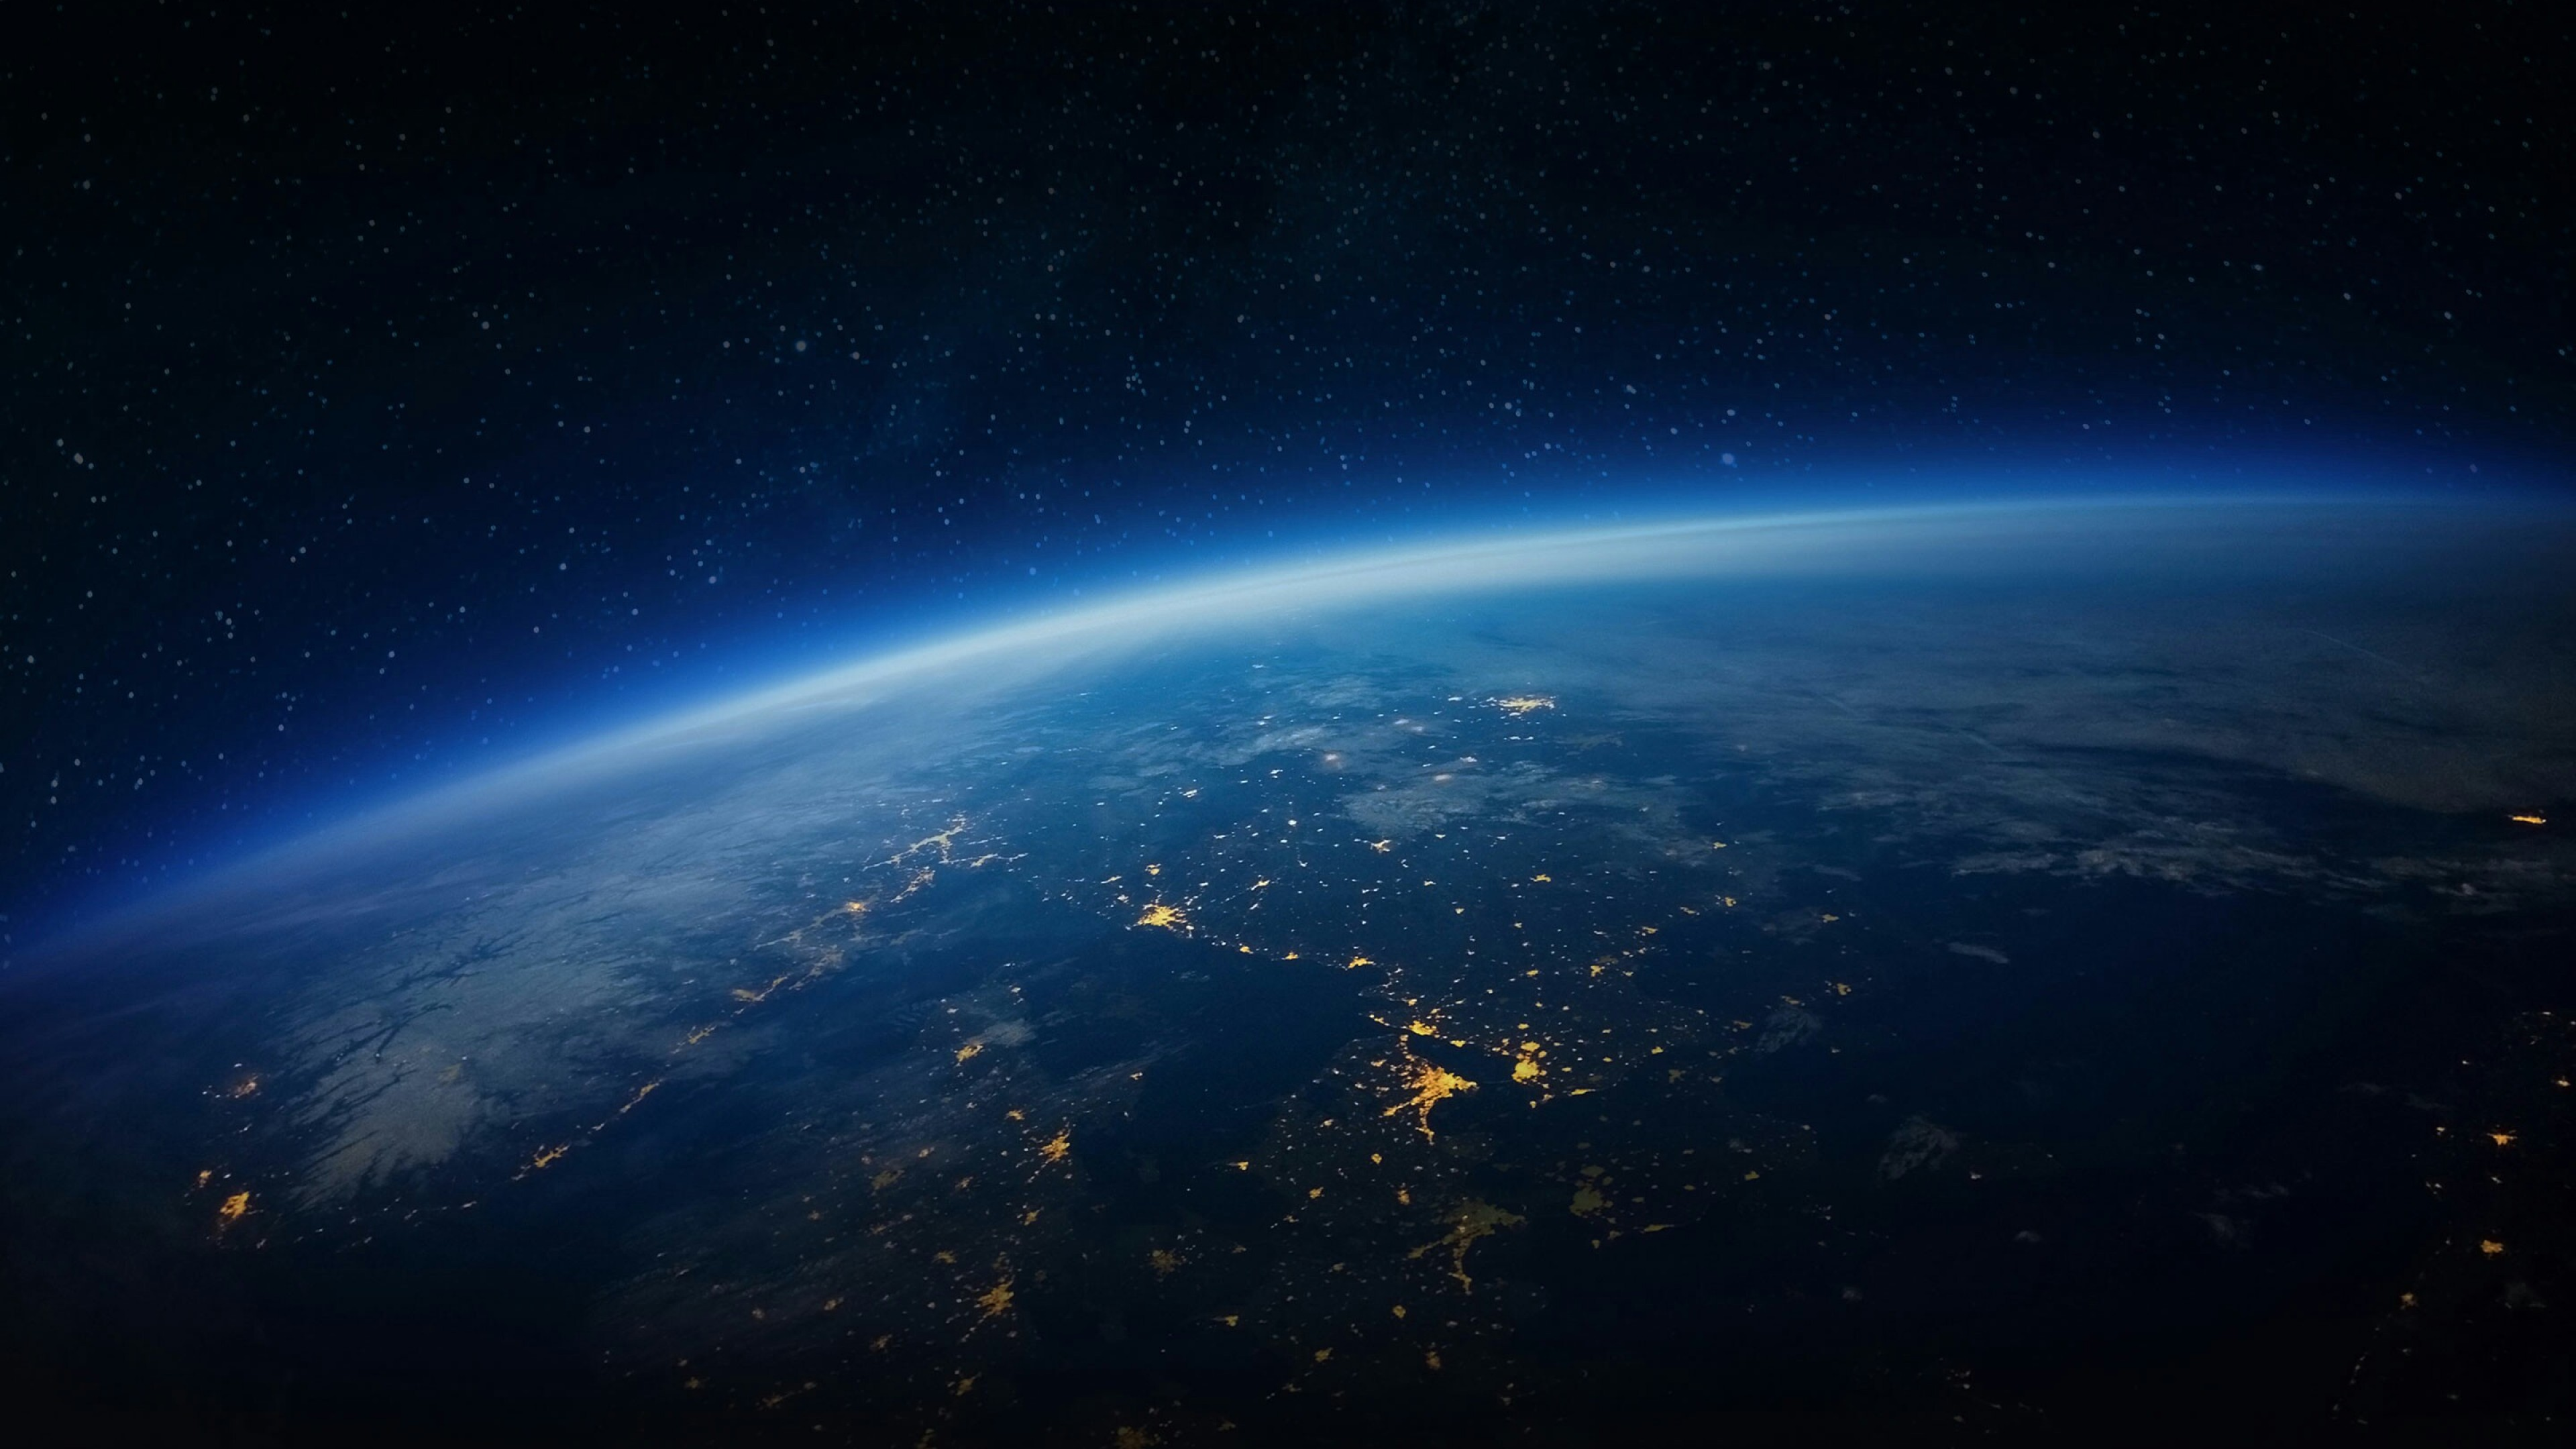
\includegraphics[scale=0.37]{head1}}} 
\centering
\vspace*{5cm}
\par\normalfont\fontsize{35}{35}\sffamily\selectfont
\textbf{{\color{white} Neuronale Netzwerke und Clusteringverfahren zur Analyse von Geodaten}}\\
{\LARGE {\color{white}Lehrstuhl für Geoinformatik}}\par
\vspace*{1cm}
{\Huge {\color{white} Robin Bially}}\par 
\endgroup

%----------------------------------------------------------------------------------------
%	COPYRIGHT PAGE
%----------------------------------------------------------------------------------------

\newpage
~\vfill
\thispagestyle{empty}

%Hier kann ich Github und Downloads hin schreiben
\noindent \textsc{https://github.com/RobinBia/Projektarbeit-Geoinformatik.git}\\ \\ % URL

\noindent Projektarbeit unter der Betreuung von PD Dr. Dr.-Ing. Wilfried Linder von 11.2017 - 12.2018 zur Vorbereitung der sich anschließenden Masterarbeit.\\ % 

\noindent \textit{Fertigstellung, Dezember 2018} 


%----------------------------------------------------------------------------------------
%	TABLE OF CONTENTS
%----------------------------------------------------------------------------------------
\raggedright
\chapterimage{head8}
\pagestyle{empty} 
\tableofcontents 
\pagestyle{fancy} 


%----------------------------------------------------------------------------------------
%	CHAPTER 1
%----------------------------------------------------------------------------------------

\chapterimage{head8} % Chapter heading image
\chapter{Motivation}
Die folgende Projektarbeit liefert einen groben Überblick über Methoden und Algorithmen im Bereich der geoinformationsverarbeitenden Systeme in Verbindung mit Machine Learning (ML). Darunter werden sämtliche Verfahren verstanden, die auf Basis von Datenbeständen Fähigkeiten erlernen, mithilfe derer abstraktere Probleme automatisiert gelöst werden können. Die Projektarbeit beschränkt sich auf die ML-Teilbereiche Deep Learning und Data Mining, welche sich mit der Wissensextraktion (Assoziationsmustererkennung), der Klassifikation und dem Clustering von Datenpunkten auseinandersetzen. Die Auswertung geowissenschaftlicher Fachliteratur soll zudem Erkenntnisse über weitere Einsatzbereiche von Machine Learning liefern. Außerdem soll recherchiert werden, worin die Herausforderungen bestehen und welche offenen Probleme es gibt.
\\~\\
Ziel der Arbeit ist die Eingrenzung der Themenbereiche auf Fragestellungen, die sich für eine wissenschaftlichen Ausarbeitung im Rahmen der sich anschließenden Masterarbeit eignen.

%----------------------------------------------------------------------------------------
%	CHAPTER 2
%----------------------------------------------------------------------------------------
\chapter{Geodaten und Geoinformation}

\section{Definition und Gestalt von Geodaten}
Geodaten sind digitale Informationen, welche Sachdaten mit Geometriedaten\footnote{https://www.hdm-stuttgart.de/~riekert/lehre gis.pdf} (und Chronometriedaten) vereinen , z.B. \{Luftdruck 1 bar, Ort Düsseldorf, Datum 26.11.2017\}. 
Die räumliche Information kann in unterschiedlichen Formen vorliegen, z.B. symbolisch als Ortsname oder Postleitzahl, aber auch als mathematisch atomare Referenz auf Positionen der Erde mittels Koordinaten. Diese können in unterschiedlichster Dimensionalität vorliegen\footnote{http://www.mathematik.uni-ulm.de/sai/ws04/biosem/GIS.pdf}:
\begin{itemize}
\item Ein Objekt ohne bestimmte Länge (0D)
\item Ein Linienstück (1D)
\item
Gauß-Krüger oder geografische Koordinaten mit Bezug auf die Oberfläche der Erde ohne Berücksichtigung von Höhenunterschieden (2D)
\item 
2D-Koordinaten mit einer zusätzlichen Sachinformation für die Höhe über dem Geoiden (2.5D).
\item Kugelkoordinaten mit Bezug auf jeden Punkt im Volumen der Erde als
Geoid oder Rotationsellipsoid (3D)
\item 
Zusätzlich zu den 3 Koordinaten im Raum wird eine vierte
Information mitgeführt, die sich aus dem zeitlichen Ablauf ergibt (4D)
\end{itemize}

Im Anhang wird in den Zeilen 2-4 ein solcher Datensatz mittels \textit{pyplot} visualisiert.

\newpage

\section{Geografische Koordinaten}
Ein geeignetes und weit verbreitetes Koordinatensystem für die verzerrungsarme Darstellung von Geodaten sind die geografischen Koordinaten. 

\begin{figure}[H]
\centering
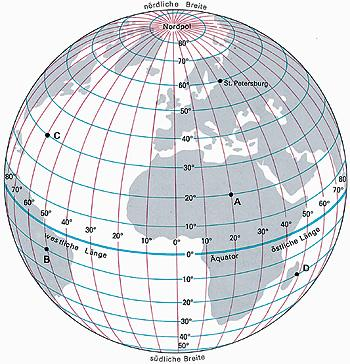
\includegraphics[scale=0.7]{gradnetz.jpg}
\caption{Das Gradnetz der Erde}\label{gradnetz}
\end{figure}

Beschrieben wird ein Punkt auf der Erde durch gedachte Kreise um den Globus, welche senkrecht zueinander stehen. Insgesamt existieren 180 Breitenkreise (Richtung Ost-West) und 360 Längenkreise (Richtung Nord-Süd). Die Abweichung von den beiden Referenzkreisen Äquator und Nullmeridian, wird in Grad östlicher/westlicher Länge und nördlicher/südlicher Breite angegeben. Als Äquator ($0^\circ$ nördliche/südliche Breite) wird der Breitenkreis bezeichnet, auf dem die Erdachse senkrecht steht. Der Nullmeridian ($0^\circ$ westliche/östliche Länge) ist der Längenkreis, der durch die britische Stadt Greenwich verläuft.\newline Weitere wichtige Koordinatensysteme sind die Gauß-Krüger und UTM-Koordinaten. Ein Vorteil dieser Systeme ist, dass sich geografische Positionen direkt ablesen lassen. Geografische Koordinaten hingegen erschweren dies bedingt durch die sich verändernden Abstände zwischen den Längenkreisen in zunehmender Nord- oder Südrichtung.


\section{Qualitätsmerkmale}
Ein wichtiger Forschungszweig ist die automatische Beurteilung von Qualitätsmerkmalen von Geodaten hinsichtlich einer bestimmten Fragestellung.
Ein geeignetes Maß für die Datenqualität ist die gewichtete Summe verschiedener Merkmale, welche in der aktuellen ISO-Norm \textit{ISO 19157:2013}\footnote{https://www.iso.org/standard/32575.html} spezifiziert sind.

Die Beurteilung der Datenqualität ist ebenfalls in sämtlichen Verarbeitungsschritten des KDD-Prozessmodells \cite{kddmod} erforderlich. Das KDD-(Knowledge Discovery in Databases-)Prozessmodell beschreibt, wie aus einer unstrukturierten Datensammlung neues, relevantes Wissen extrahiert werden kann. Es umfasst folgende Schritte:
\begin{enumerate}
\item \textbf{Fokussieren/Selektieren} Die Daten werden zusammengetragen, in Form einer Datenbank strukturiert und irrelevante Einträge werden gelöscht. Relevante Daten können bezüglich einer bestimmten Fragestellung potentiell vielversprechende Erkenntnisse liefern.
\item \textbf{Vorverarbeitung} Es wird überprüft, ob die Datenbank konsistent ist und ob es fehlende Einträge gibt. Die Konsistenz wird verletzt, wenn zum Beispiel einer Koordinate ein Land zugeordnet wird, welches den umgebenen Datenpunkten nicht zugeordnet wurde. Die Wahrscheinlichkeit einer Fehlzuordnung ist dann groß. Die Datenbank hat fehlende Einträge, wenn es Attribute mit nicht existierenden Werten gibt. Strategien zum Umgang mit fehlerhaften Datensätzen beim Clustering werden in Kapitel 4 erläutert.
\item \textbf{Transformation} Wurde ein komplexes Objekt in die Datensammlung aufgenommen, so müssen seine Merkmale zuerst numerisch diskretisiert werden. Beispielsweise hat ein Reisfeld eine Länge und Breite, aber auch eine Vegetationsdichte und einen Erntestatus. All diese Merkmale müssen vermessen und in die Datenbank aufgenommen werden. Merkmale, welche nach der Transformation in mangelhafter Qualität vorliegen, können entfernt werden.
\item \textbf{Data Mining} Methoden zur Mustererkennung. Dazu gehören sowohl Neuronale Netze und Clusteringverfahren, als auch Assoziationsregeln.
\item \textbf{Evaluation} Ergebnisse der Mustererkennung werden statistisch überprüft und die Nützlichkeit vom Nutzer bewertet.
\end{enumerate}~\\


\begin{figure}[H]
\centering
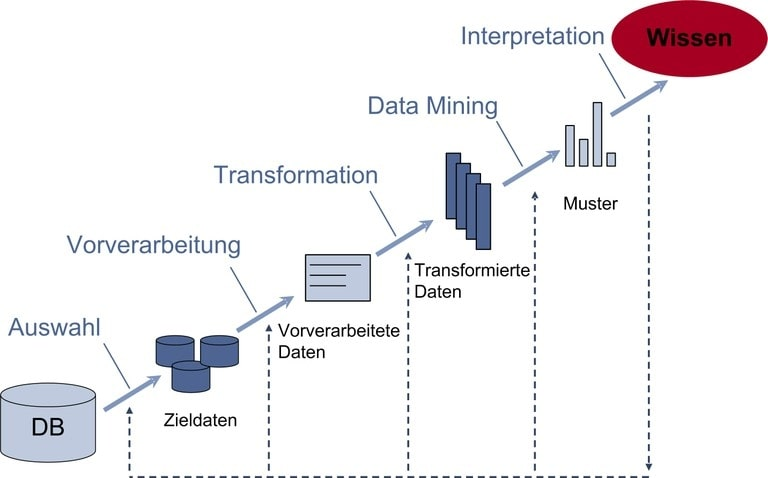
\includegraphics[scale=0.35]{kdd.jpg}
\caption{Das KDD-Prozessmodell \protect\footnotemark}
\end{figure}
\footnotetext{\url{http://www.enzyklopaedie-der-wirtschaftsinformatik.de/lexikon/daten-wissen/Business-Intelligence/Analytische-Informationssysteme--Methoden-der-/Data-Mining/index.html}}


Die folgende Auflistung ist eine informelle Beschreibung der oben genannten ISO-Norm \textit{ISO 19157:2013} durch Fragestellungen und Beispiele:

\begin{itemize}
\item \textbf{Vollständigkeit}
\begin{itemize}
\item \textbf{Datenüberschuss} -
Enthält der Datensatz mehr Objekte und Beziehungen als angegeben?
\item \textbf{Datenmangel} - Enthält der Datensatz weniger Objekte und Beziehungen als angegeben?
\end{itemize}
\item \textbf{Logische Konsistenz}
\begin{itemize}
\item \textbf{Konzeptuelle Konsistenz} - 
Ist die Gestalt des Datenmodells nach Aktualisierungen gleich geblieben?
\item \textbf{Wertekonsistenz} - Sind alle Werte sinnvoll?
\item \textbf{Formatkonsistenz} Passen die Daten zu angegebenen physikalischen Einheiten?
\item \textbf{Topologische Konsistenz} 
Bleiben topologische Beziehungen bei Änderungen des Datensatzes bestehen (Der botanische Garten befindet sich im Umkreis von 1km um die HHU)?
\item \textbf{Geometrische Konsistenz} - Ist der digitalisierte Datensatz geometrisch sinnvoll und widerspruchsfrei?
\end{itemize}
\item \textbf{Positionsgenauigkeit}
\begin{itemize}
\item
\textbf{Äußere Genauigkeit} - Wie gut stimmen die Koordinatenwerte des Datensatzes mit den wahren Koordinaten überein?
\item \textbf{Innere Genauigkeit} - Wie gut stimmen die relativen Positionen von Objekten zueinander mit den wahren relativen Positionen überein?
\item \textbf{Rasterdatengenauigkeit} - Wie gut stimmen die Rasterdatenpositionswerte mit den wahren Werten überein?
\end{itemize}
\item \textbf{Zeitliche Genauigkeit}
\begin{itemize}
\item
\textbf{Genauigkeit von Zeitmessungen} - 
Wie genau ist die Zeitangabe (minutengenau, taggenau)?
\item \textbf{Zeitliche Konsistenz} - Ist die Reihenfolge der Ereignisse korrekt?
\item
\textbf{Zeitliche Gültigkeit} - Ist der Datensatz in Bezug auf das geforderte Zeitformat korrekt?
\end{itemize}
\item \textbf{Thematische Genauigkeit}
\begin{itemize}
\item
\textbf{Richtigkeit der Klassifikation} - Stimmen Objekte oder ihre Attribute mit den zugewiesenen Klassen überein?
\item \textbf{Richtigkeit nichtquantitativer Attribute} - Beispiel: Ist das Grundstück wirklich eine Bananenplantage?
\item \textbf{Genauigkeit quantitativer Attribute} - Beispiel: Ist die Fläche des Grundstücks korrekt?
\end{itemize}
\end{itemize}

Viele der oben genannten Punkte lassen einen subjektiven Spielraum für die Bewertung zu. Sowohl Skalierungen als auch Gewichtungen sind nicht eindeutig definiert, was einen Vergleich verschiedener Datensätze erschwert. Aus diesem Grund könnte eine algorithmische Interpretation in Kombination mit Verfahren der künstlichen Intelligenz hilfreich sein. Im besten Fall ließe sich aus der oben genannten Norm ein universeller und allgemeingültiger Indikator zur Bewertung der Datenqualität ableiten.


\section{Georeferenzierung}
\subsubsection{Definition}
Unter dem Vorgang der Georeferenzierung,versteht man die Zuweisung raumbezogener Informationen (auch Georeferenz genannt) zu einem Datensatz.

Es gibt folgende vier Arten der Georeferenzierung:

\begin{itemize}
\item Bei der \textbf{Adresskodierung} wird dem Datensatz eine Postanschrift zugewiesen und somit ein indirekter Raumbezug hergestellt. Mithilfe geokodierter Adressen lassen sich funktionale zusammenhänge zwischen Daten, Postanschrift und Adresse herstellen. Auf diese Weise können ressourcenschonende und schnelle Zugriffe ermöglicht werden.
\item Als \textbf{Geotagging} bezeichnet man das Einfügen eines Attributes (Geotag) inkl. Realweltkoordinate in einen raumbezogenen Datensatz wie ein Bild oder eine Website. Dies ist bei der räumlichen Einordnung der Information hilfreich.
\item Bei der \textbf{Kartenkalibrierung} wird ein räumlicher Datensatz ohne Realkoordinatenbezug mithilfe einer Transformationsvorschrift im Bezug auf die Realwelt so orientiert, dass sich die Koordinaten des Bildes in Realweltkoordinaten einfach umrechnen lassen.
\item Bei der \textbf{Rektifizierung} werden geometrische Verzerrungen in räumlichen Daten entzerrt, indem jedem Datum eine Realweltkoordinate zugeordnet wird.
\end{itemize}


\subsubsection{Bestimmung einer Transformationsvorschrift}

Um eine Transformationsgleichung zu finden, werden in der Regel Passpunkte verwendet. Passpunkte müssen im Datensatz eindeutig zu erkennen sein. Die Koordinaten der Passpunkte im Realweltkoordinatensystem sind entweder bekannt oder werden einem Referenzdatensatz entnommen. Bei Vorliegen von Vektordaten werden die Koordinaten abgegriffen oder interpoliert. Bei Bilddaten hingegen werden die Bildkoordinaten der Passpunkte gemessen. Die Transformation sollte unter Berücksichtigung der Abbildungsgeometrie bestimmt werden. Bei Fotos ist somit die Zentralprojektion zu berücksichtigen, bei Karten der entsprechende Kartennetzentwurf. Das automatische Finden von Gemeinsamkeiten in digitalen Bildern und die Bestimmung der Transformation wird in der Bildverarbeitung Bildregistrierung genannt. Die Registrierung von Laserscanning-Punktwolken kann mit dem ICP-Algorithmus durchgeführt werden.\footnote{https://de.wikipedia.org/wiki/Georeferenzierung}


\section{Geoinformationssysteme}
Ein Geoinformationssystem ist eine Software, mit welcher Geodaten erfasst, verwaltet, analysiert und ausgegeben werden können.

Man unterscheidet bei der Abfrage von Daten zwischen folgenden Typen:
\begin{itemize}
\item Alphanumerische Daten (Attribute als Text oder Zahlen)
\item Text-Dokumente 
\item Multimediale Informationen, wie Videos, Audiosequenzen, Animationen 
\item Fotos, Scans, Satellitenbilder
\end{itemize}

Der Unterschied zu einer Datenbank ist, dass jedes Sachdatum einen expliziten Raumbezug hat, über den die Selektion erfolgt. In einer Datenbank erfolgen Zugriffe stattdessen über Schlüsselattribute. Eine weitere Stärke von GIS ist die grafische Aufbereitung der Daten zur anschaulich-interaktiven Analyse.

Beispiele für solche räumlichen Analysewerkzeuge sind die Routenfindung und räumliche Suche. Ein Kartografiesystem ermöglicht zudem das Markieren von Punkten und Linien, Färben von Flächen und die Anzeige und Überlagerung verschiedener Ebenen.

\subsection{Geoobjekte}
Ein Geoobjekt ist ein tatsächlich auf der Erde vorhandenes Objekt, das durch Geodaten eindeutig referenziert wurde. Man unterscheidet zwischen Gegenständen und Sachverhalten. Gegenstände sind konkrete, visuell wahrnehmbare Erscheinungen auf der Erdoberfläche. Sachverhalte dagegen sind nicht visuell wahrnehmbar, sondern stehen für Beziehungen zwischen Gegenständen oder Interaktionen mit der Umwelt und Oberflächengestalt der Erde.
Außerdem unterscheidet man zwischen verschiedenen Arten der Datenspeicherung:
\begin{itemize}
\item Flächenhafte Daten
\item Linienhafte Daten
\item Punkthafte Daten
\end{itemize}
Je nach Kartenmaßstab, Auflösungstyp und Speichertyp (digital/analog) werden Daten unterschiedlich repräsentiert. So wird beispielsweise ein flächenhafter quadratischer Gebäudekomplex ($10 \times 10$ Meter) auf einem Satellitenfoto mit dem Maßstab $1:10000$ nur noch als Punkt wahrgenommen. Linienhafte Daten bieten sich vor allem zur Speicherung von Flüssen, Straßen, Wasser-Land-Grenzen, starken Flankensteigungen usw. an.

\subsubsection{Modellierung von Geoobjekten}
Die vier informationstechnischen Dimensionen zur Modellierung von geografischen Informationssystemen sind:
\begin{itemize}
\item Geometrie (Ort des Objekts)
\item Topologie (Lage der Objekte relativ zueinander)
\item Semantik (Bedeutung des Objekts im fachspezifischen Kontext, z.B. gut-schlecht, viel-wenig, groß-klein)
\item Dynamik (Änderung des Objekts im zeitlichen Verlauf)
\end{itemize}
Jedes unikate Objekt gehört zu einer Objektklasse, in der es nach den oben genannten vier Kriterien beschrieben und mit anderen Objekten der Klasse verglichen wird. Jedes der Objekte besitzt einen eindeutigen Schlüssel zur Identifikation. Möglichkeiten zur Klassifizierung und Gruppierung von Geoobjekten werden in den folgenden Kapiteln vorgestellt.\newline
Der Ort eines Geoobjekts kann im Raster- oder Vektormodell beschrieben werden:

\subsection{Rastermodell}
Eine analoge topografische Karte oder Zeichnung digitalisiert und in quadratische Gitterzellen aufgeteilt, welche alle über die gleiche Semantik verfügen. Diese Semantik wird stellvertretend durch eine Matrix beschrieben, die für jede Gitterzelle eine numerische Pixelwertinformation enthält.\footnote{https://de.wikipedia.org/wiki/Geoobjekt}
\begin{figure}[H]
\centering
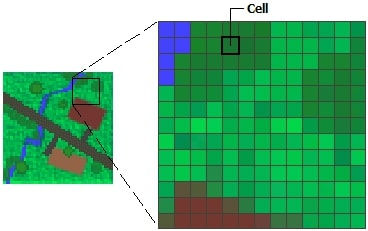
\includegraphics[scale=0.5]{raster.jpg}
\caption{Rastermodell-Zoom \protect\footnotemark}
\end{figure}
\footnotetext{http://desktop.arcgis.com/de/arcmap/10.3/manage-data/raster-and-images/what-is-raster-data.htm}

Pixelwerte repräsentieren Daten wie Temperatur, Höhe, Vegetationsdichte, Landnutzung und Bodenbeschaffenheit. Rasterdaten werden in der Regel als Bilddatei gespeichert (BMP, GIF, JPEG, PNG).
\newline
Die Rastergeometrie eignet sich gut zur Beschreibung flächiger, homogener Sachverhalte. Die einfache Struktur bietet viele Vorteile, aber auch Nachteile. \newline
\textbf{Vorteile:}
\begin{itemize}
\item Einfache Datenstruktur 
\item Geeignet für räumliche und statistische Analyse
\item Alles ist einheitlich speicherbar (Punkte, Linien, Polygone)
\item Überlagerung von Ebenen sehr schnell und einfach
\end{itemize}
\textbf{Nachteile:}
\begin{itemize}
\item Genauigkeitsverlust beim Scannen und Neustrukturieren
\item Endliche Auflösung $\Rightarrow$ räumliche Ungenauigkeit
\item Pixelwerte haben keine Beziehung zueinander
\item Hoher Speicheraufwand bei Hoher Auflösung, keine Kompression möglich.
\end{itemize}

\subsection{Vektormodell}
Im Gegensatz zu Rasterdaten werden Vektordaten bei linien- und punkthaften Informationen eingesetzt, also Informationen, die sich nicht mit homogener Eigenschaft über die gesamte Karte verteilen. Man nennt solche Informationen auch Features. Beispiele hierfür sind Straßen, Staatsgrenzen, Gewässergrenzen, Höhenlinien, Flüsse, Bäume.
\newline
Eine punkthafte Vektorinformation wird auch als Vertex bezeichnet. Dieser beschreibt eine Raumlage durch Angabe einer (x,y,z)-Koordinate und ein dazugehöriges Attribut, das die Art des Punktes beschreibt (z.B. Baum oder Laterne):

\begin{figure}[H]
\centering
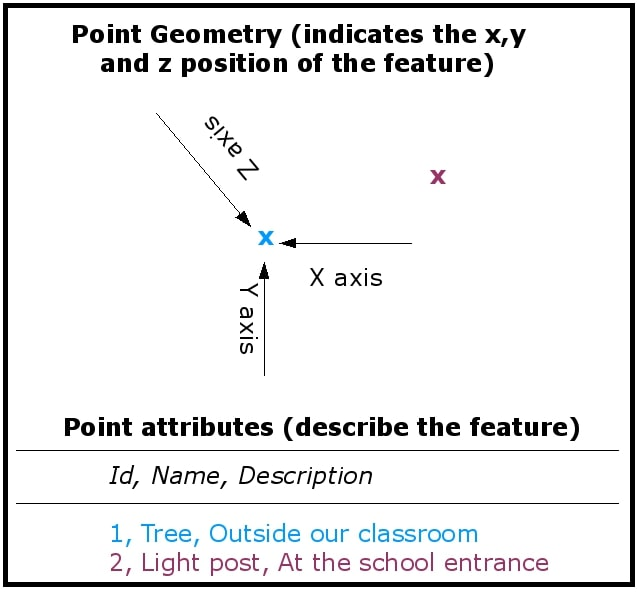
\includegraphics[scale=0.3]{vertex.jpg}
\caption{Punkt-Feature \protect\footnotemark}
\end{figure}

\footnotetext{https://docs.qgis.org/2.8/de/docs/gentle\_gis\_introduction/vector\_data.html}

Punkteverläufe wie Straßen werden durch sogenannte Polylinien beschrieben. Diese bestehen aus mehreren miteinander verbundenen Vertices. Im Kreis laufende Polylinien bezeichnet man auch als Polygone:

\begin{figure}[H]
\centering
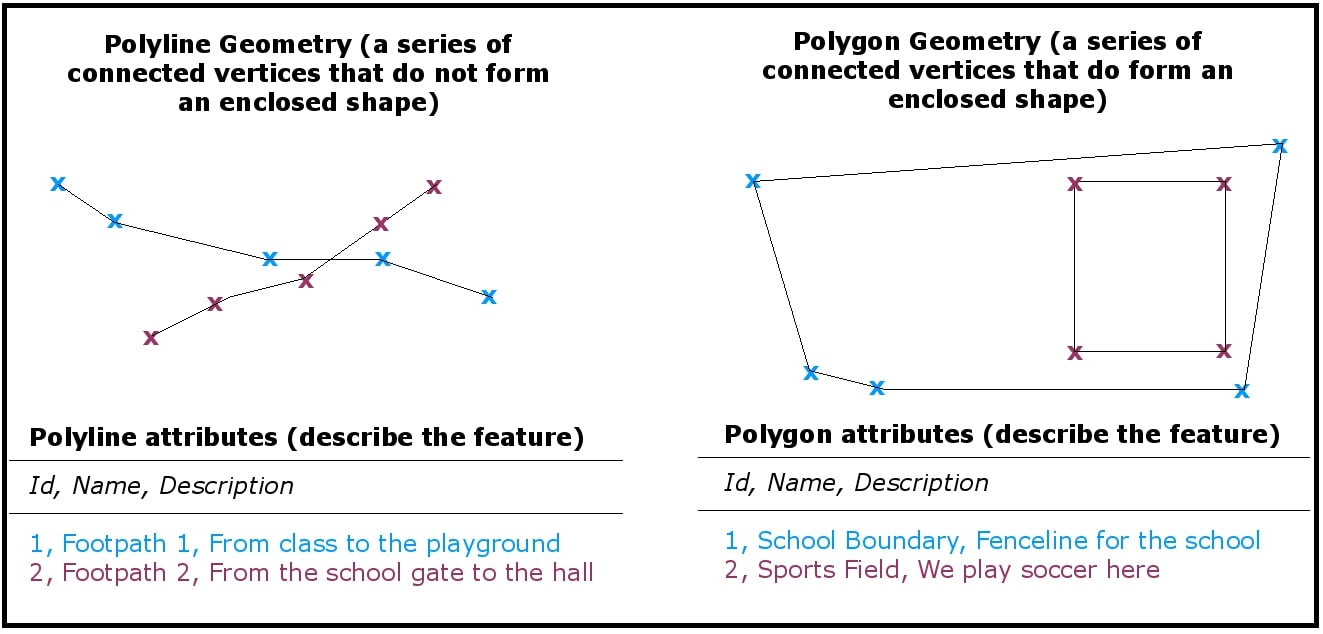
\includegraphics[scale=0.3]{poly.jpg}
\caption{Polylinien und Polygone \protect\footnotemark}
\end{figure}

\footnotetext{https://docs.qgis.org/2.8/de/docs/gentle\_gis\_introduction/vector\_data.html}

Vektordaten haben wie die Rasterdaten sowohl Vorteile, als auch Nachteile.\footnote{http://romanharcke.de/geoinformationssysteme-geodaten-kapitel-4/}\newline
\textbf{Vorteile:}
\begin{itemize}
\item Unendliche Linienauflösung und sehr hohe Genauigkeit
\item Beschreibung von mehreren einzigartigen Features in nur einer Ebene möglich
\item Geringer Speicherbedarf
\item Einfache Erzeugung von Topologie (Knoten, Kanten, Flächen)
\item Gute Performance
\item Ermöglicht Attributierung und Objektdefinitionen
\end{itemize}
\textbf{Nachteile:}
\begin{itemize}
\item Flächenhafte Informationen können nicht gespeichert werden 
\item Durch Scannen können diese Daten nicht erzeugt werden. Es bedarf hier einer Raster-Vektorwandlung (Hoher Erfassungsaufwand)
\item Hoher Rechenaufwand bei Verschneidungen
\end{itemize}

\subsection{Beispiele für Raster und Vektordaten}
Geodaten müssen heutzutage nicht mehr selbständig erstellt werden. Es gibt eine Vielzahl an staatlichen und privaten Institutionen, welche ihre Daten kostenlos bereitstellen. So lassen sich zahlreiche Inhalte im ESRI-Shapefile Vektordateiformat finden, das als Quasi-Standard für Desktop-GIS gilt.\footnote{\url{http://webhelp.esri.com/arcgisdesktop/9.3/index.cfm?TopicName=Geoprocessing\%20considerations\%20for\%20shapefile\%20output}}
Der Datensatz \textit{Natural Earth}\footnote{http://www.naturalearthdata.com/} ist eine Abbildung der Erde im Maßstab $1:10$ Millionen. Er ist sowohl als SHP-Vektordatei als auch als Tiff-Rasterbild verfügbar.

Ein ESRI-Shapefile besteht aus mindestens drei Dateien. Diese speichern Geometriedaten, Sachdaten und die Geometrieindizierung zur Verknüpfung von Geometrie und Sachdaten (.shp, .dbf, .shx). Die Geometrie eines Shapefile definiert sich aus nur vier verschiedenen Formdatenstrukturen: Punkte, Linien, Flächen (Polygone) und Multipunkte.\footnote{http://www.esri.com/library/whitepapers/pdfs/shapefile.pdf}

\begin{figure}[H]
\centering
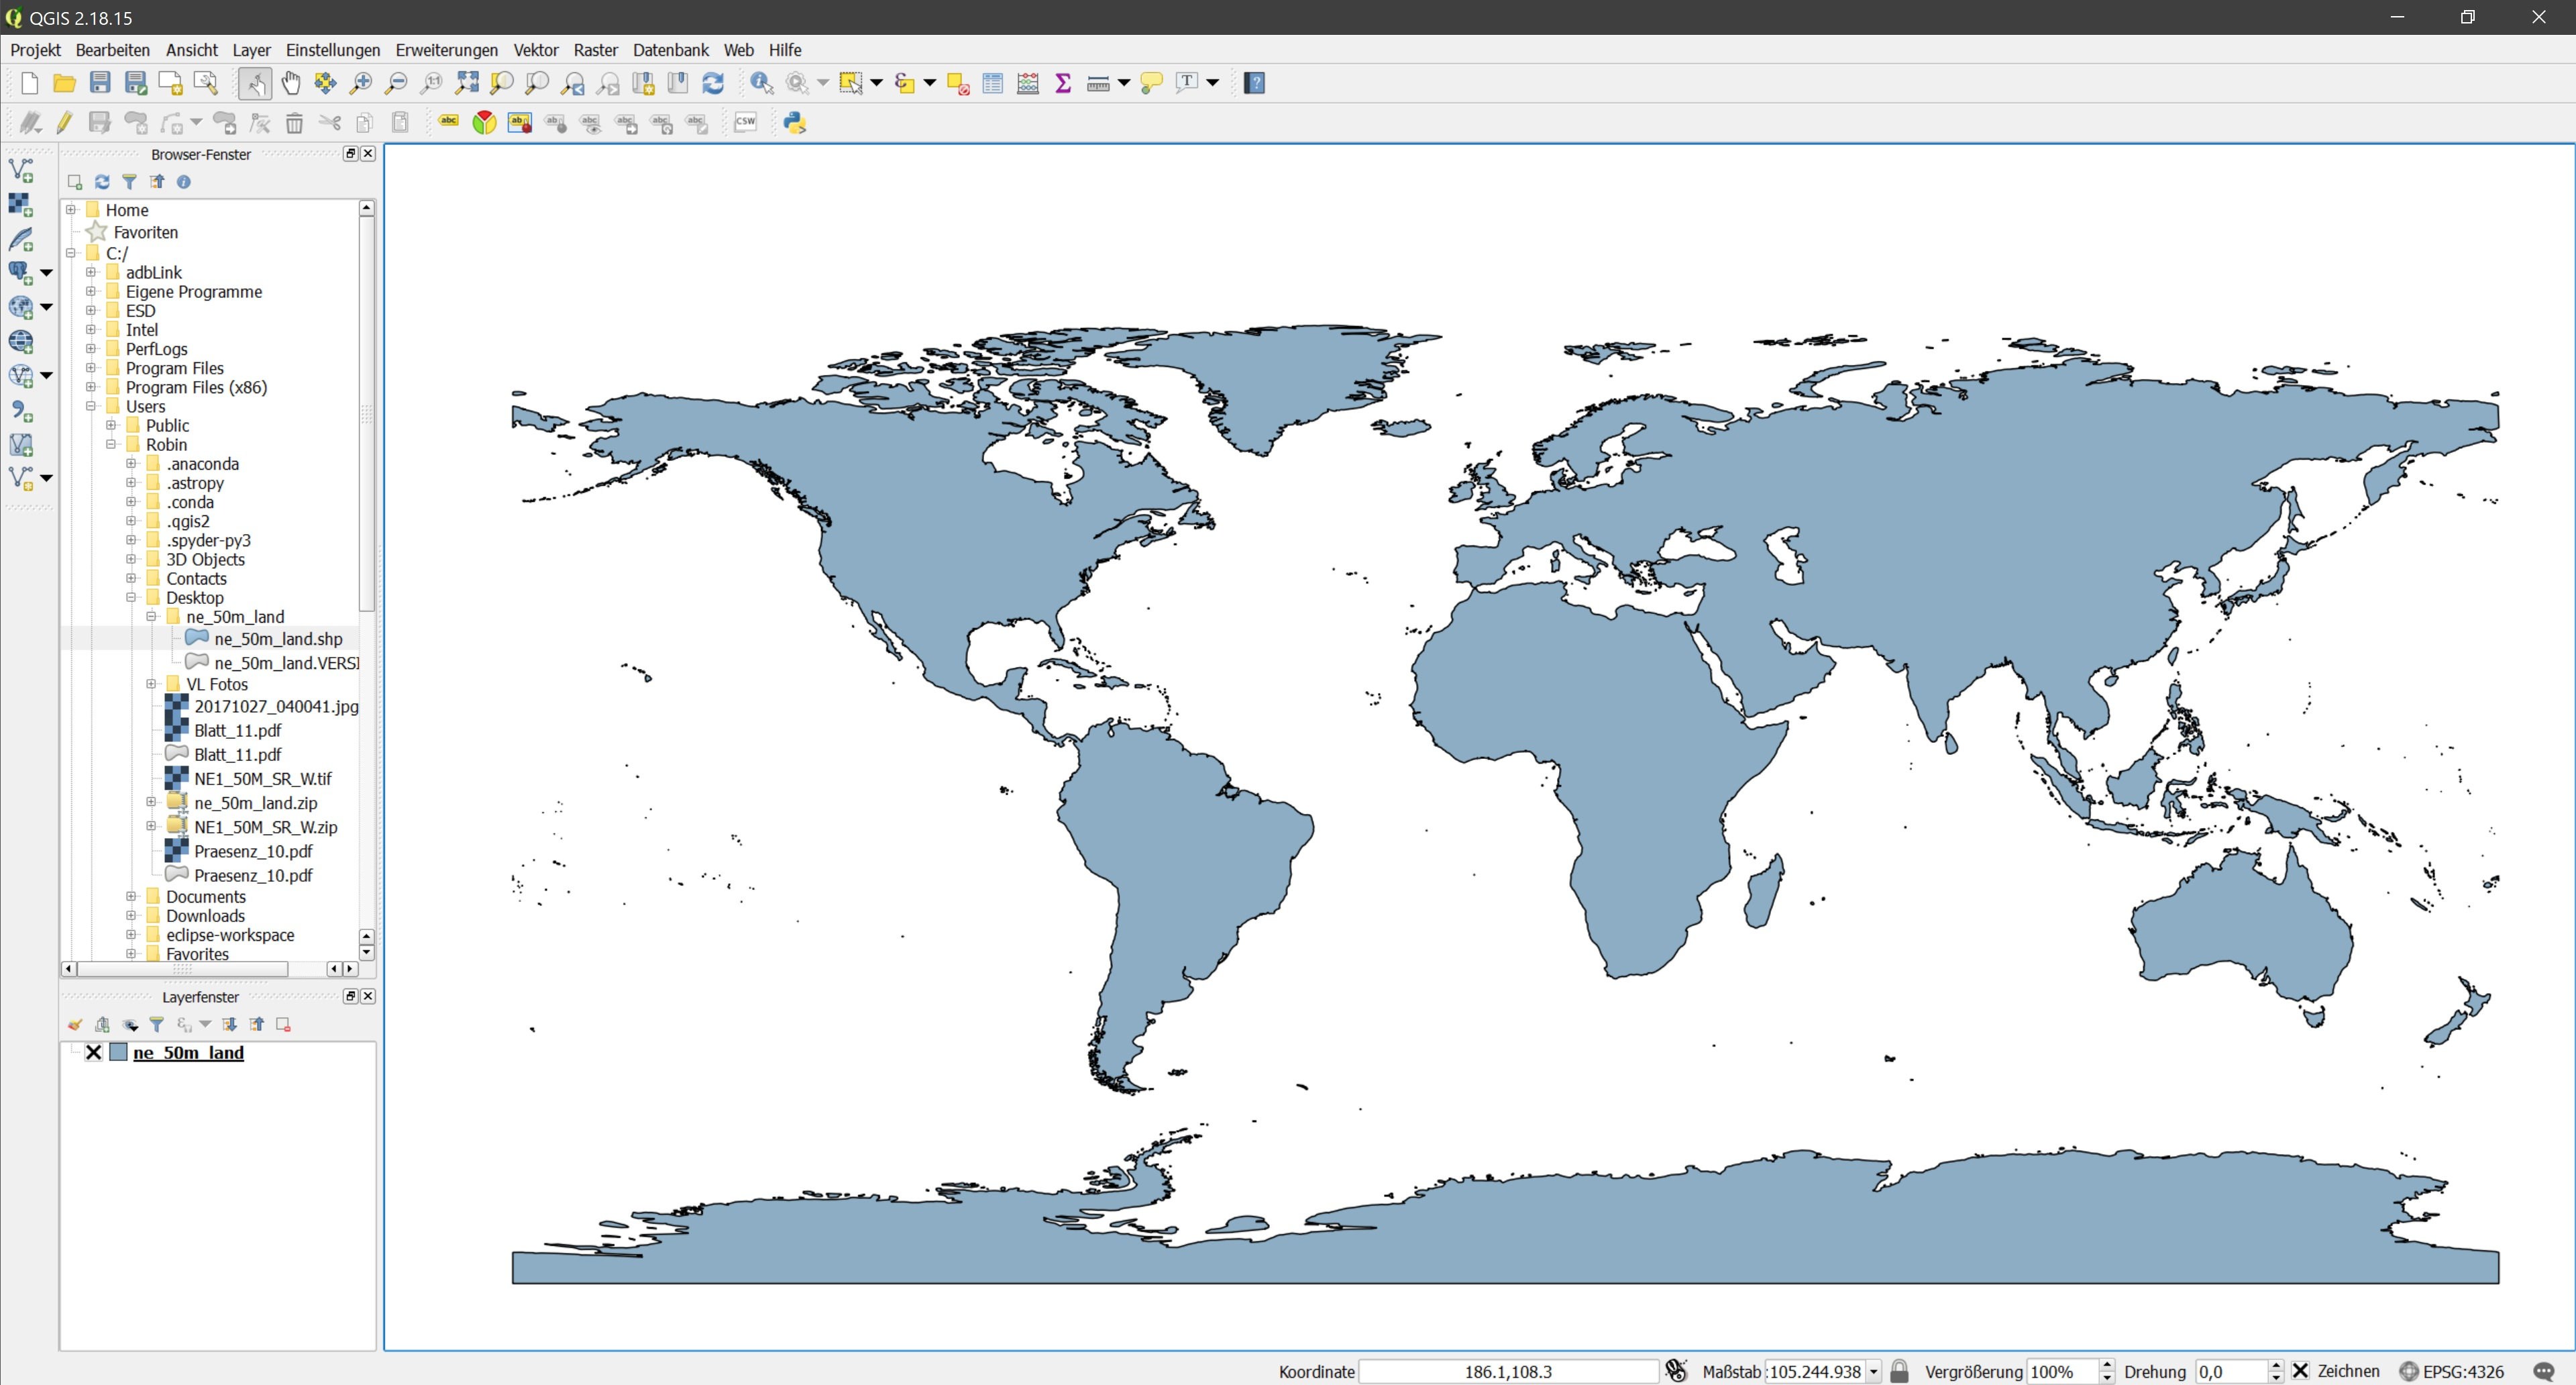
\includegraphics[scale=0.23]{gis.jpg}
\caption{.shp-Geometriedatei in dem Geoinformationssystem QGIS dargestellt \protect\footnotemark}
\end{figure}
\footnotetext{https://www.qgis.org/de/site/}
Leider eignen sich Vektordaten nicht zur Klassifikation von Features mithilfe von z.B. Convolutional Neural Networks (CNN), sondern stellen vielmehr das Ergebnis einer Rasterbildanalyse dar. Aus diesem Grund beziehen sich folgende Kapitel im Kontext von Geodaten immer auf Rasterdaten und Bildausschnitte.
\newline
Das dem Datensatz zugehörige farbige Rasterbild inklusive Schummerung (räumliche Schattierung), Wasser und Flüssen sieht so aus:

\begin{figure}[H]
\centering
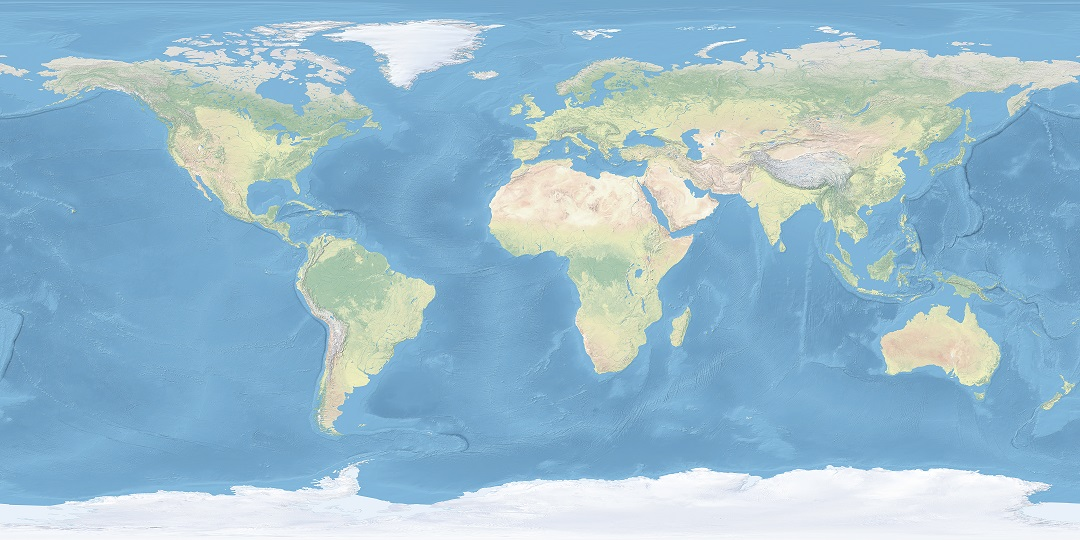
\includegraphics[scale=0.9]{raster_nat_earth.jpg}
\caption{Rasterbild des Natural-Earth-Datensatzes \protect\footnotemark}
\end{figure}
\footnotetext{http://www.naturalearthdata.com/downloads/10m-raster-data/10m-natural-earth-1/}

\section{Algorithmen in der Geoinformatik}
\section{Verschiedene Arten und ihre Anwendungszwecke}

%----------------------------------------------------------------------------------------
%	CHAPTER 3
%----------------------------------------------------------------------------------------

\chapter{Deep Learning}

\section{Was ist Machine Learning?}
\textbf{Definition}\\
Machine Learning ist eine Unterdisziplin der künstlichen Intelligenz und basiert auf der Idee, biologische Denkprozesse, wie sie in Gehirnen ablaufen, nachzuahmen \cite{geofront}.

\textit{A computer program is said to learn from experience E with
respect to some class of tasks T and performance measure P if its performance at tasks in T, as measured by P, improves with experience E.} \cite{michell}

\bigskip

Ein Computerprogramm lernt also genau dann dazu, wenn es sich hinsitlich seiner Performance in bestimmten Aufgabengebieten mithilfe von Erfahrung selbständig verbessert.

\section{Motivation und Anwendungsgebiete}
Ziel von Machine Learning in den Geowissenschaften ist es, Muster in Geodaten zu erkennen, Vorhersagen zu machen und Phänomene besser erkennen und verstehen zu können.

\bigskip
\textbf{Beispiel:}\\
Eine Stadt ist ein komplexes System, das aus vielen kleineren interagierenden Subsystemen besteht. Diese werden durch Faktoren wie Politik, Bevölkerungswachstum, Verkehrsinfrastruktur und den Arbeitsmarkt beeinflusst.
Um zu verstehen, welche Kräfte strukturelle Änderungen von Städten vorantreiben, werden sowohl Satellitenbilder als auch nutzerbezogene Positionsdaten aus sozialen Netzwerken wie Facebook und Twitter verwendet. Ebenfalls werden attributierte Markierungen auf Geoinformationssystemen wie OpenStreetMap\footnote{https://www.openstreetmap.org} verwendet, um Langzeitvorhersagen zur erstellen.
Außerdem helfen diese Modelle und Simulationen dabei, die Mechanismen der urbanen Evolution zu erforschen und Städteplanung zu optimieren.


%\clearpage
\vspace*{\fill}
\begin{center}
\begin{minipage}{1\textwidth}
Es folgt eine Auflistung verschiedener Probleme, für deren Lösung sich die Anwendung eines Neuronalen Netzwerks eignet:

\begin{itemize}
\item Klassifizierung - Was ist auf einem Bild zu sehen?
\item Lokalisation - Wo ist das Objekt auf dem Bild?
\item Segmentierung - Klassifizierung jedes Pixels
\item Lineare Regression - Lässt sich ein funktionaler Zusammenhang zwischen den Daten des Datensatzes finden, welcher eine Vorhersage zum weiteren Verlauf der Daten ermöglicht?
\item Clustering - Wie lassen sich Daten vergleichen und in Anbetracht ihrer Attributähnlichkeiten in Gruppen zusammenfassen?
\item Image Captioning - Wie lassen sich die klassifizierten Objekte in Beziehung setzen? 
\end{itemize}

\end{minipage}
\end{center}
\vfill
\clearpage
\clearpage

\begin{figure}[h]
\centering
\vfill
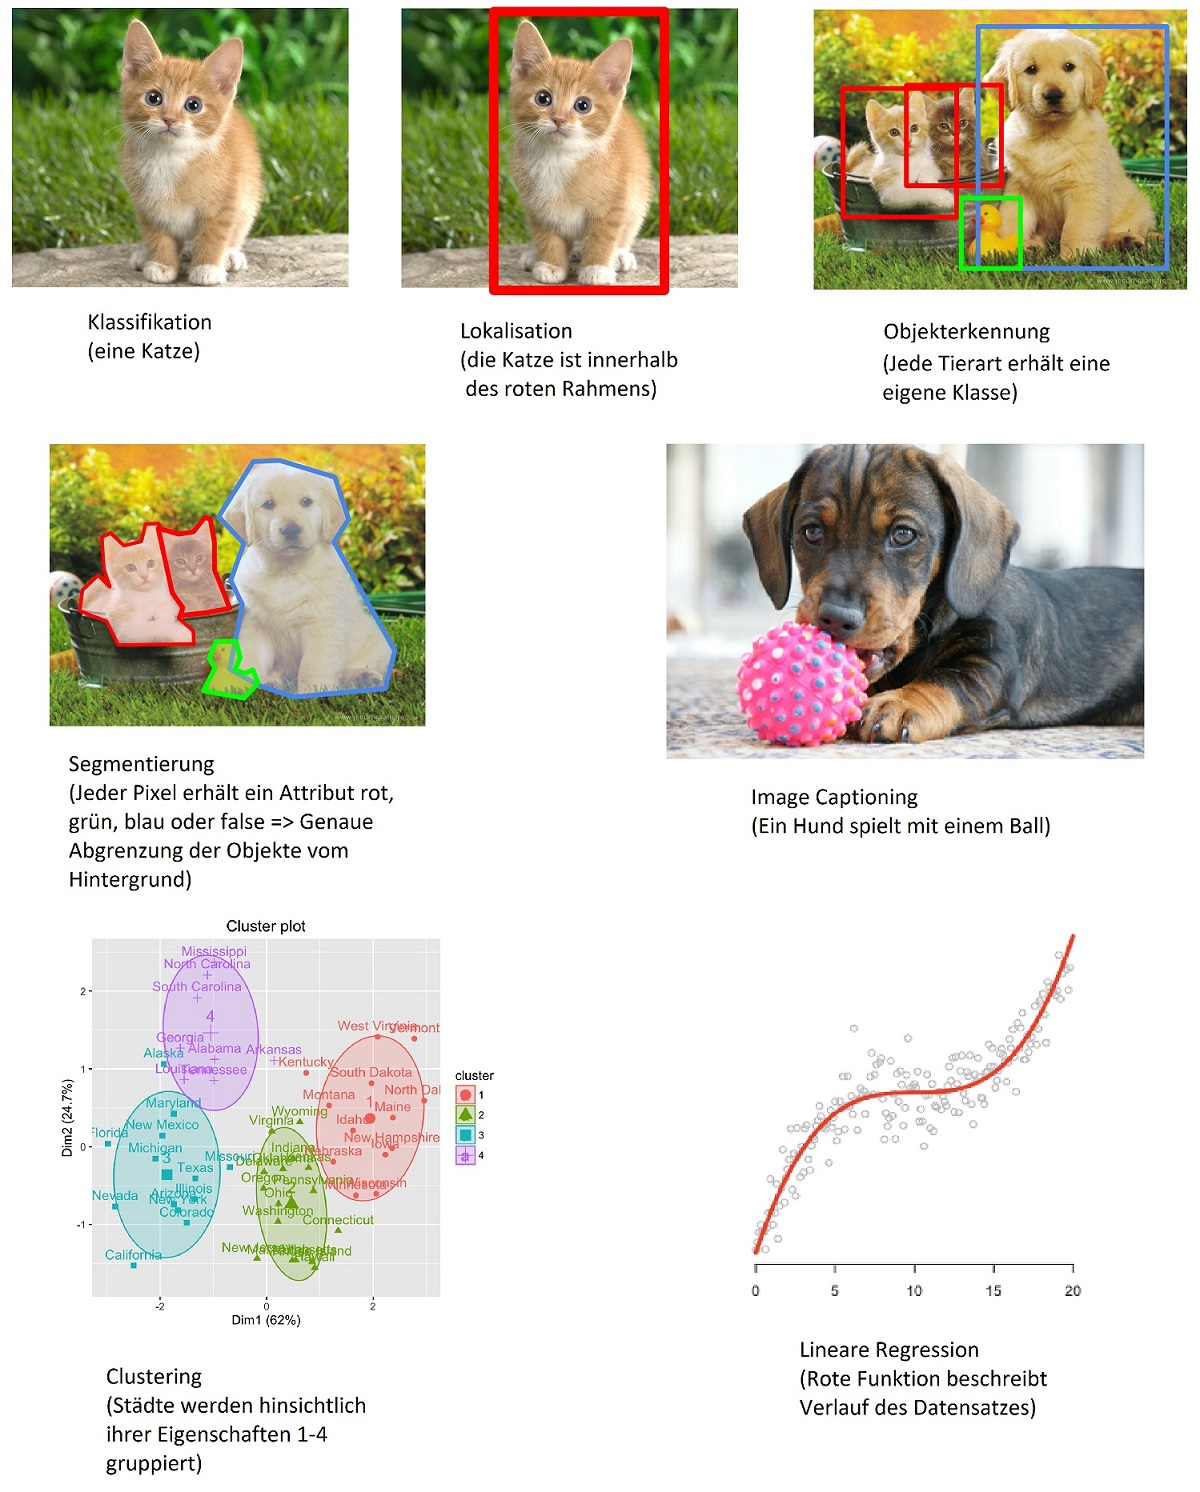
\includegraphics[scale=0.77]{anwendungen.jpg}
\caption{Vergleich verschiedener Anwendungszwecke von Deep Learning}
\vfill
\end{figure}
\clearpage 


\subsection{Linear Classifier}
Um bestimmen zu können, wie gut ein Bild $x$ ($x_i$ sind die einzelnen Pixelwerte) zu einer Klasse $k_j$ passt, muss mithilfe einer Funktion $f$ ein numerischer Vergleichswert bestimmt werden. Die Funktion $f$ wird auch Score-Funktion genannt:
$$f(x_i, W, b) = W \cdot x_i + b$$
Der Parameter $W$ ist die sogenannte Gewichtsmatrix. Sie besitzt die Dimensionalität $i_{max} \times k_{max}$.
Der Parameter $b$ heißt Bias und besitzt die Dimensionalität $k_{max} \times 1$. Er hat die gleiche Funktion wie die Gewichtsmatrix, ermöglicht aber eine zusätzliche additive Änderung beim Lernen. Im nächsten Unterkapitel wird genauer Erläutert, wie dies zu interpretieren ist.

\begin{figure}[H]
\centering
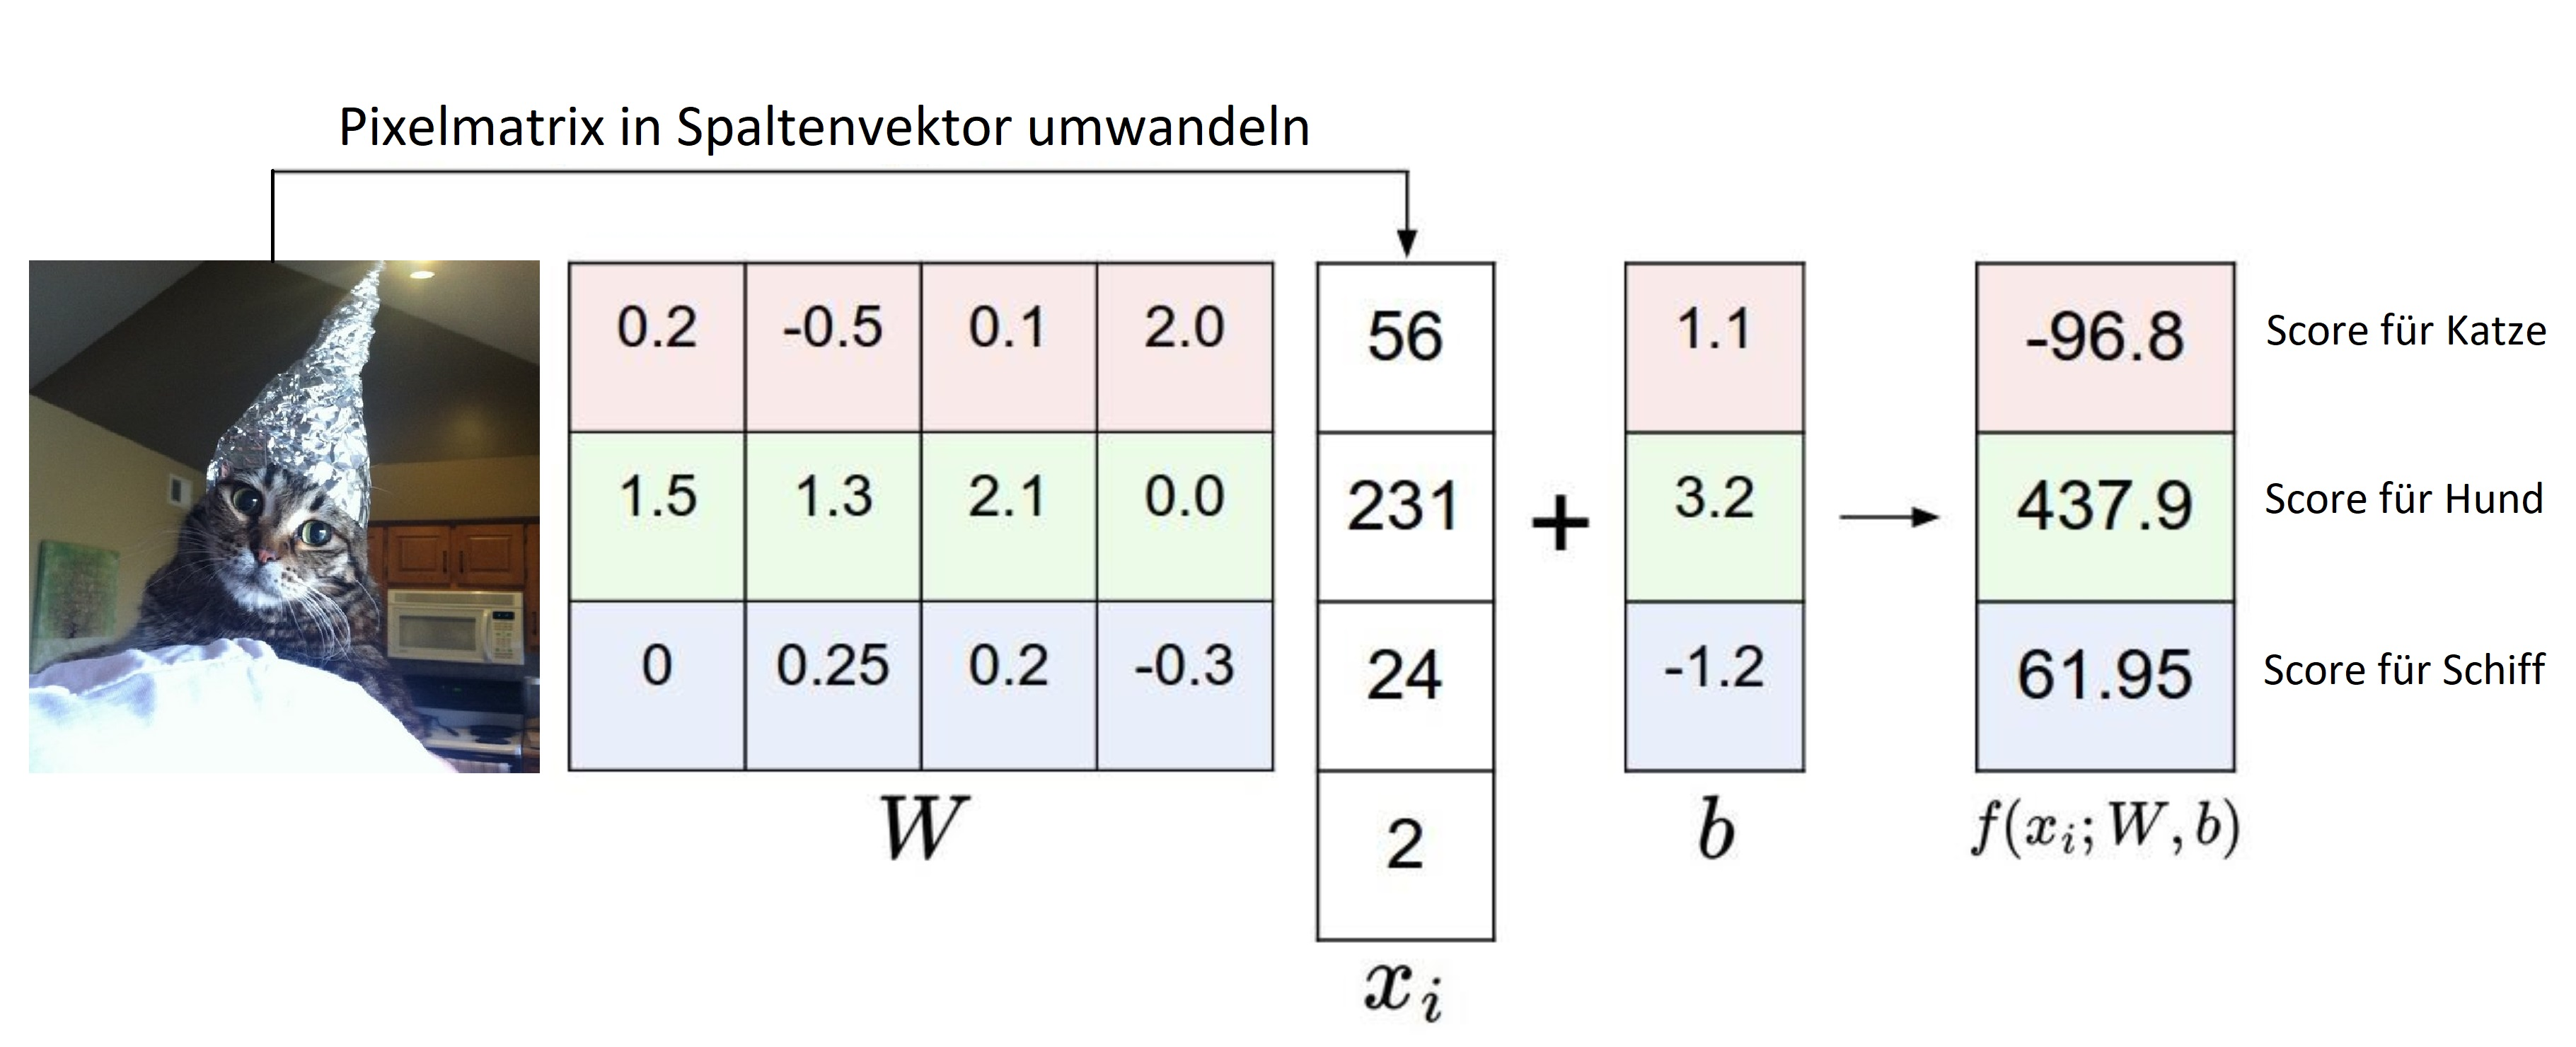
\includegraphics[scale=0.25]{wxplusb.jpg}
\caption{Interpretation der Score-Funktion anhand eines Beispiels}
\end{figure}

Wenn man ein Bild mit $i_{max}$ Pixeln als $i_{max}$-dimensionalen Vektor auffasst, dann lässt sich ein Classifier als Hyperebenenseparator dieses Vektorraumes interpretieren. Je höher die Score-Funktion für eine Klasse, desto geringer ist der Abstand zum Untervektorraum mit entsprechenden zur Klasse gehörenden Mustern.

\begin{figure}[H]
\centering
\includegraphics[scale=0.3]{hyperraum.jpg}
\caption{Hirsch-Auto-Flugzeug-Hyperraum mit Ebenenseparatoren}
\end{figure}

Äquivalent zur Score-Funktion definiert man auch eine sogenannte Loss-Funktion. Je besser ein Datum einer bestimmten Klasse zugeordnet werden kann, desto besser sind die Parameter der Gewichtsmatrix und des Bias und desto kleiner ist der Wert der Loss-Funktion. Im Rahmen eines Optimierungsprozesses soll die Loss-Funktion durch Änderung der Gewichte minimiert werden.
\bigskip
Zwei häufig verwendete Loss-Funktionen für Daten sind:
\begin{itemize}
\item \textbf{Hinge-Loss} $L_i = \sum\limits_{j \neq y_i} max\left(0,s_j - s_{y_i} + \Delta\right) \Rightarrow$ Richtige Klasse muss um mindestens Delta größer sein, als alle anderen Klassen
\item \textbf{Softmax-Loss} $L_i = -\log\left(\frac{e^{s_{y_i}}}{\sum_{j} e^{s_j}}\right) \Rightarrow$ Minimieren der negativen logarithmischen Wahrscheinlichkeit für die korrekte Klasse
\end{itemize}

Der gesamte Loss eines Optimierungsproblems besteht jedoch nicht nur aus dem oben genannten Data-Loss, sondern des Weiteren aus dem Regularisierungs-Loss.

\subsection{Regularisierer}
Ein Regularisierer soll verhindern, dass sich die Gewichte immer nur hinsichtlich einer bestimmten Klasse verändern. Zum Beispiel kann es sein, dass ein Netzwerk, das ohne Regularisierer trainiert wurde, zwar gut Katzen erkennen kann, jedoch keine Hunde. Das Ziel ist hierbei also, ein Netzwerk zu erzeugen, das die Generalisierung "Tier" versteht und darüber hinaus zwischen verschiedenen Tierarten unterscheiden kann. Eine Möglichkeit, dies zu realisieren, bieten Bestrafungsterme:

\[R(W) = \sum_{k}\sum_{l} W_{k,l}^2\]

Dieser Bestrafungsterm geht ebenfalls in die Loss-Funktion mit ein. Die Quadrierung der Gewichte sorgt dafür, dass zuvor bereits deutlich größere Gewichte in der Loss-Funktion umso mehr berücksichtigt werden. Im Laufe des Trainingsprozesses können Ausreißer effektiv erkannt und vermieden werden. Die Loss-Funktion wird nur dann minimal sein, wenn sich die Gewichte nicht zu stark voneinander unterscheiden.
\\
Die gesamte Loss-Funktion lautet also:
\[L_{ges} = \frac{1}{N} \sum_{i} L_i + \lambda R(W)\]

\subsection{Gradientenabstieg}
Um die Loss-Funktion zu minimieren, müssen die Gewichte $W$ aktualisiert werden. Hierzu berechnet man den negativen Gradienten, also die partiellen Ableitungen der Loss-Funktion nach den Gewichten. Auf der Ebene, welche die Loss-Funktion aufspannt, zeigt der Gradient in Richtung des steilsten Abstiegs.


\subsection{Multi-Layer Neural Network}
Ein Multi-Layer Neuronales Netzwerk ist ein gerichteter azyklischer Graph, wobei die Knoten in Ebenen angeordnet werden. Die erste Knotenebene besteht aus den Eingabedaten. Im Bildbeispiel wäre jeder Knoten ein Pixelwert. Die Kanten des Graphen entsprechen den Werten der Gewichtsmatrix $W$. Die Knoten der Hidden-Layers unter der Output-Layer lassen sich als Neuronen interpretieren, welche durch Aktivierung oder Deaktivierung bestimmte Muster der Eingabedaten lernen. Ob ein Neuron aktiviert wird oder nicht, bestimmt die Aktivierungsfunktion $g$. Das Ergebnis wird an eine weitere Neuronenschicht weitergeleitet und die gelernten Muster somit weiter verfeinert.

\begin{figure}[H]
\centering
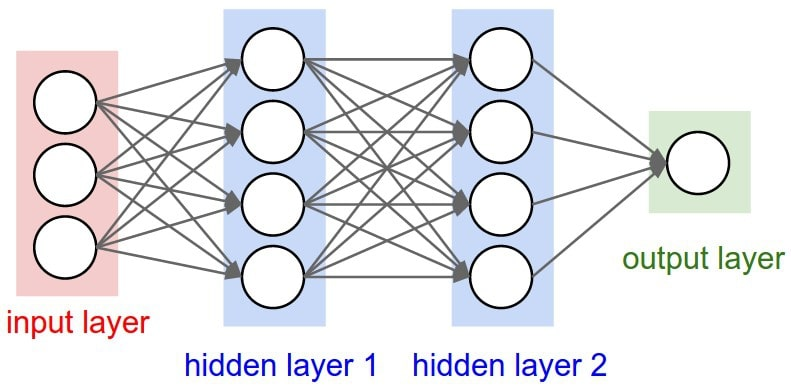
\includegraphics[scale=0.35]{mlnn.jpg}
\caption{Multi-Layer NN. mit 2 Hidden-Layers, 32 Gewichten, 9 Biases und 9 Neuronen}
\end{figure}

Die Score-Funktion für dieses Netzwerk lautet:

\[y(x) = W_3^{\top} \cdot g[W_2^{\top} \cdot g[W_1^{\top} \cdot x+b_1]+b_2]+b_3\]


\subsection{Trainieren eines Netzwerks mittels Backpropagation}
Sei $f$ eine Score-Funktion für ein Single Layer Neural Network mit nur einer Aktivierung.

\[f(x,w) = \frac{1}{1+e^{-(w_0x_0+w_1x_1+w_2)}}\]

Diese Aktivierungsfunktion nennt sich auch Sigmoidfunktion. Sie transformiert reelle Zahlen auf ein Intervall $\left[0, 1\right]$.

\begin{figure}[H]
\centering
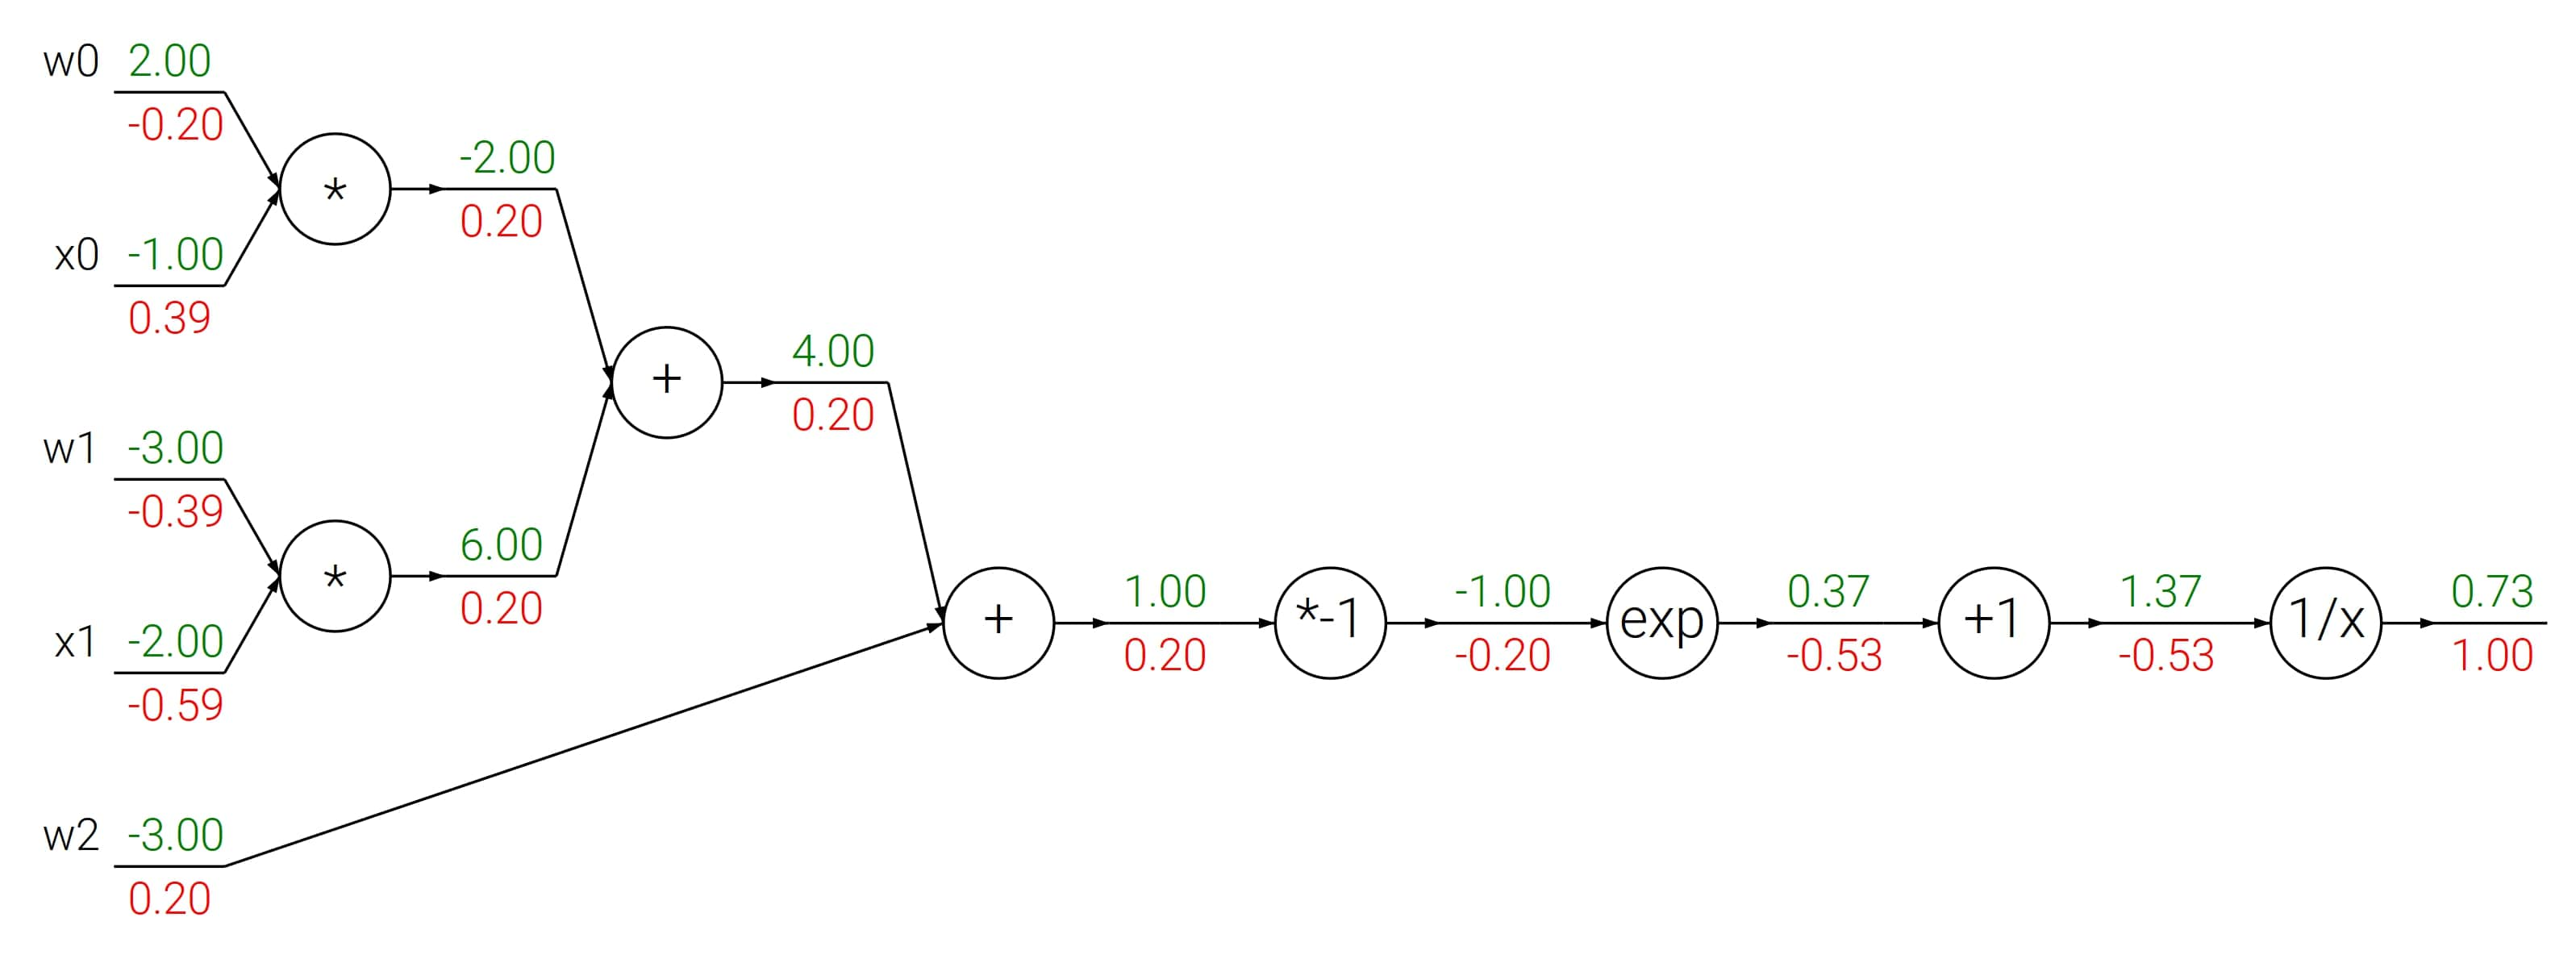
\includegraphics[scale=0.12]{sigmoid.jpg}
\caption{Beispiel für Backpropagation anhand der Sigmoid-Funktion}
\end{figure}

Das Ergebnis von $f(x,w)$ mit $w = (2,-1,-3)$ und $x = (-1,-2)$ ist $0.73$. Die Ableitung von  $\frac{1}{x}$ ist $-\frac{1}{x^2}$. Anschließend rechnet man $-\frac{1}{1.37^2}\cdot 1 = -0.53$. Die Ableitung von $x+1$ ist $1$. Also rechnet man $1\cdot -0.53=-0.53$. Die Ableitung von $e^x$ ist $e^x$. Man rechnet $e^{-1}\cdot 0.53=-0.2$. Diese Vorgehensweise entspricht der Anwendung der Kettenregel. Fährt man fort, erhält man Gewichtsänderungen $W_{exch}=(-0.2,-0.4,0.2)$. Diese Änderungen subtrahiert man von den alten Gewichten mit einem Parameter $step$: $W \minuseq step \cdot W_{exch}$. Dabei gibt die Lernrate $step$ an, wie stark die Änderung der Gewichte ausfallen soll. Eine zu große Änderung kann bedeuten, dass man über das Minimum der Loss-Funktion hinaus springt. Sind die Änderungen zu klein, so muss der Gradient oft berechnet werden, was sehr lange dauern kann. Das Ergebnis der Score-Funktion für $W' = (1.8,-3.4,-2.8)$ ist $0.9$. Das Netzwerk klassifiziert nun also besser.\\

Neben der Sigmoidfunktion gibt es noch viele andere Aktivierungsfunktionen. So hat die Maximumsfunktion (Rectifier Linear Unit - ReLU) gegenüber der Sigmoidfunktion den Vorteil, dass bei relativ hohen Werten nicht alle Neuronen aktiviert werden und es somit weiterhin zu einem Lerneffekt kommt. Ein weiterer Vorteil des Rectifier ist die schnellere Konvergenz des Gradienten. So stellt sich bereits nach wenigen Trainings ein starker Lerneffekt ein. Sind die Gewichte jedoch zu Beginn sehr klein, so ist die Gefahr groß, dass bei einer weiteren Verkleinerung alle Neuronen deaktiviert werden.

\begin{figure}[H]
\centering
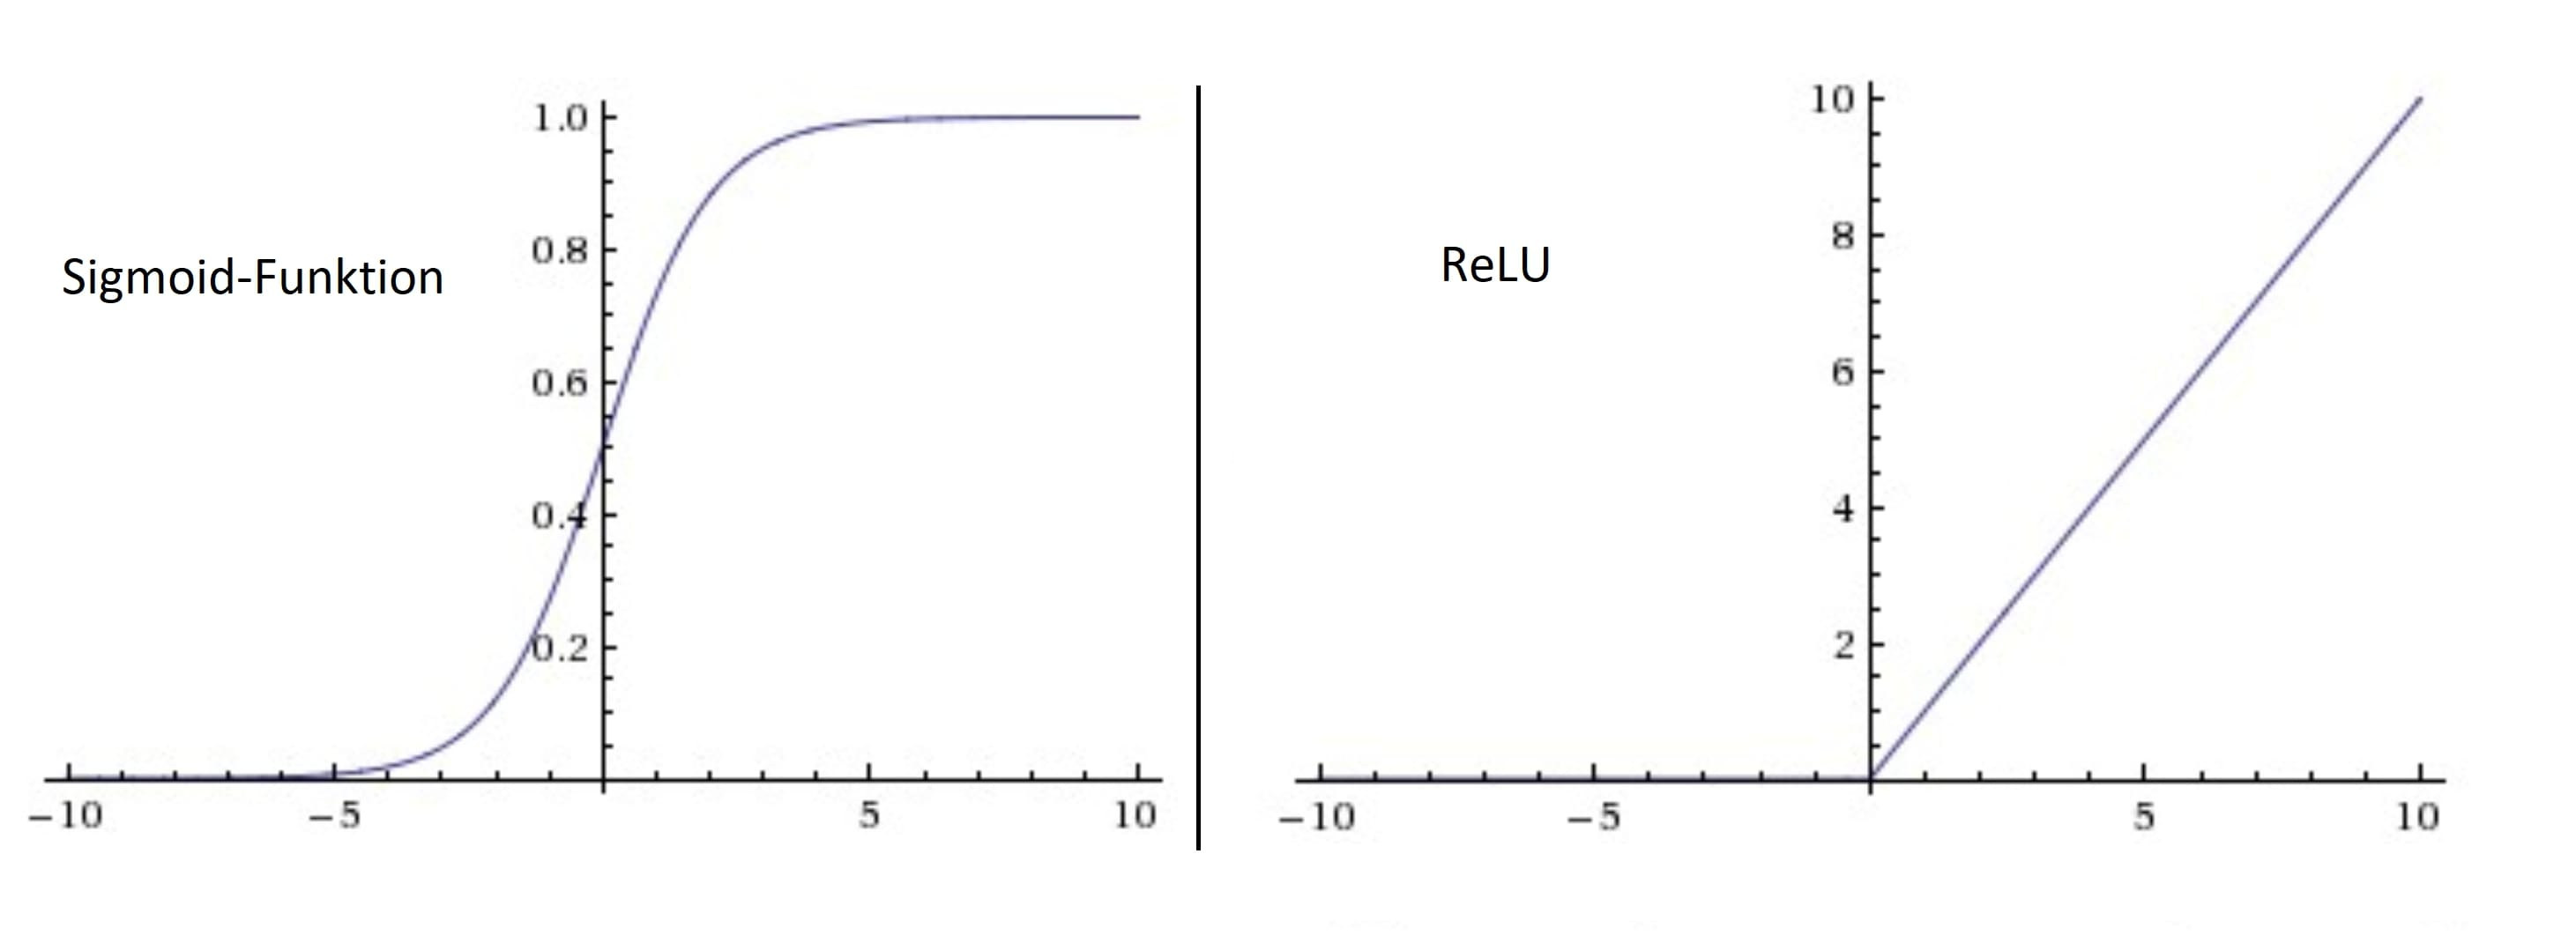
\includegraphics[scale=0.15]{aktf.jpg}
\caption{Vergleich zwischen Rectifier und Sigmoid}
\end{figure}

\subsection{Parameterupdates}
Die folgenden Verfahren sind die Grundlegendsten und am häufigsten eingesetzten Methoden zur Aktualisierung der Gewichte. Aus ihnen sind viele weitere Optimierungen hervorgegangen, die auch in der heutigen Forschung noch intensiv diskutiert werden \cite{gdalg}.\\~\\

\textbf{Batch Gradient Descent (BGD)}
Normaler einmaliger Updateprozess wie oben beschrieben. Diese Variante ist sehr langsam, da für jedes Update der Gradient für den gesamten Datensatz berechnet werden muss.
\[W = W - \eta \nabla_WL(W)\]

\textbf{Stochastic Gradient Descent (SGD)}
In diesem Fall werden die Gewichte nach jedem Trainingsbeispiel aktualisiert. Dies beschleunigt den Trainingsprozess und verhindert Redundanzen:

\[W=W - \eta \nabla_W L(W;x_i)\]

\bigskip
Zur Beschleunigung des Gradientenabstiegs wurden ebenfalls Verfahren entwickelt:
\begin{itemize}
\item \textbf{Momentum} Falls der Gradient zu groß ist, wird das Ziel beim Aktualisieren der Gewichte übersprungen. Diese Methode beschleunigt den Gradientenabstieg, indem die Anzahl der übersprungenen Minima reduziert wird (quantitative Oszillationsreduktion). Hierzu wird der Update-Vektor des vorherigen Schrittes durch einen Parameter $\gamma$ gewichtet und zum neuen Update-Vektor addiert:

\[v_t=\gamma v_{t-1}+\eta \nabla_WL(W)\]
\[W=W-v_t\]

\begin{figure}[H]
\centering
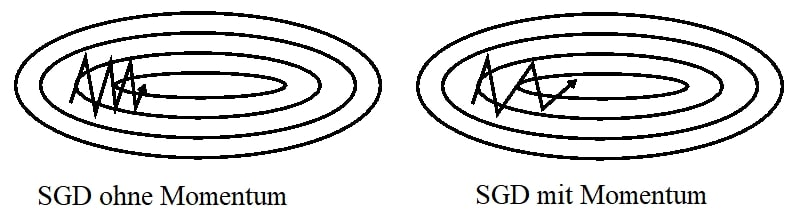
\includegraphics[scale=0.35]{momentum.jpg}
\caption{Momentum verringert die Oszillation der Loss-Funktion}
\end{figure}



\item \textbf{Adagrad} Dieses Verfahren findet für jeden Parameter in jedem Updateschritt eine individuelle Lernrate. Dies bewirkt, dass das Minimum bei starker Steigung nicht übersprungen wird. Die Oszillation wird qualitativ reduziert.

\[W_{t+1,i}= W_{t,i} - \frac{\eta}{\sqrt{G_{t,ii}+\epsilon}} \nabla_W L(W_{t,i})\]

Wobei $G_{t}$ eine Diagonalmatrix ist und das Element $i,i$ ist die Summe der Quadrate der Gradienten bezüglich $W_t$ bis Zeitschritt $t$. Das $\epsilon$ verhindert eine Nulldivision.
\end{itemize}

\subsection{Convolutional Neural Network}
Ein \textit{Convnet} ist ein Neuronales Netzwerk, das speziell für das Klassifizierungsproblem geeignet ist. Ein Standardnetzwerk besteht aus folgenden vier Schichten:

\begin{itemize}
\item \textbf{1. Convolution Layer} Dies ist ein Filter $W$, der Dimension $F \times F\times c$, wobei das Bild $P$ die Dimension $N\times N\times c$ hat und $N>F$. Die neue Größe (Höhe/Breite $N$) des Ausgabebildes nach der Convolution beträgt $\frac{N-F}{stride+1}$, wobei der Stride die Anzahl der Gitterzellen ist, die der Filter jedes mal weiter springt. Als Padding bezeichnet man die Anzahl der Gitterreihen, die um das Ursprungsbild herum virtuell angefügt werden, um zu verhindern, dass das Bild durch die Convolution kleiner wird. Zu Beginn wird der Filter an die linke obere Ecke angesetzt. Anschließend wird der erste Wert des neuen Bildes berechnet.

\[\sum_{i=1}^F \sum_{k=1}^F{P_{i,k} \cdot w_{i,k}}\]

Danach wird der Filter um $stride$ Gitterzellen nach rechts verschoben und es wird erneut aufsummiert.

\begin{figure}[H]
\centering
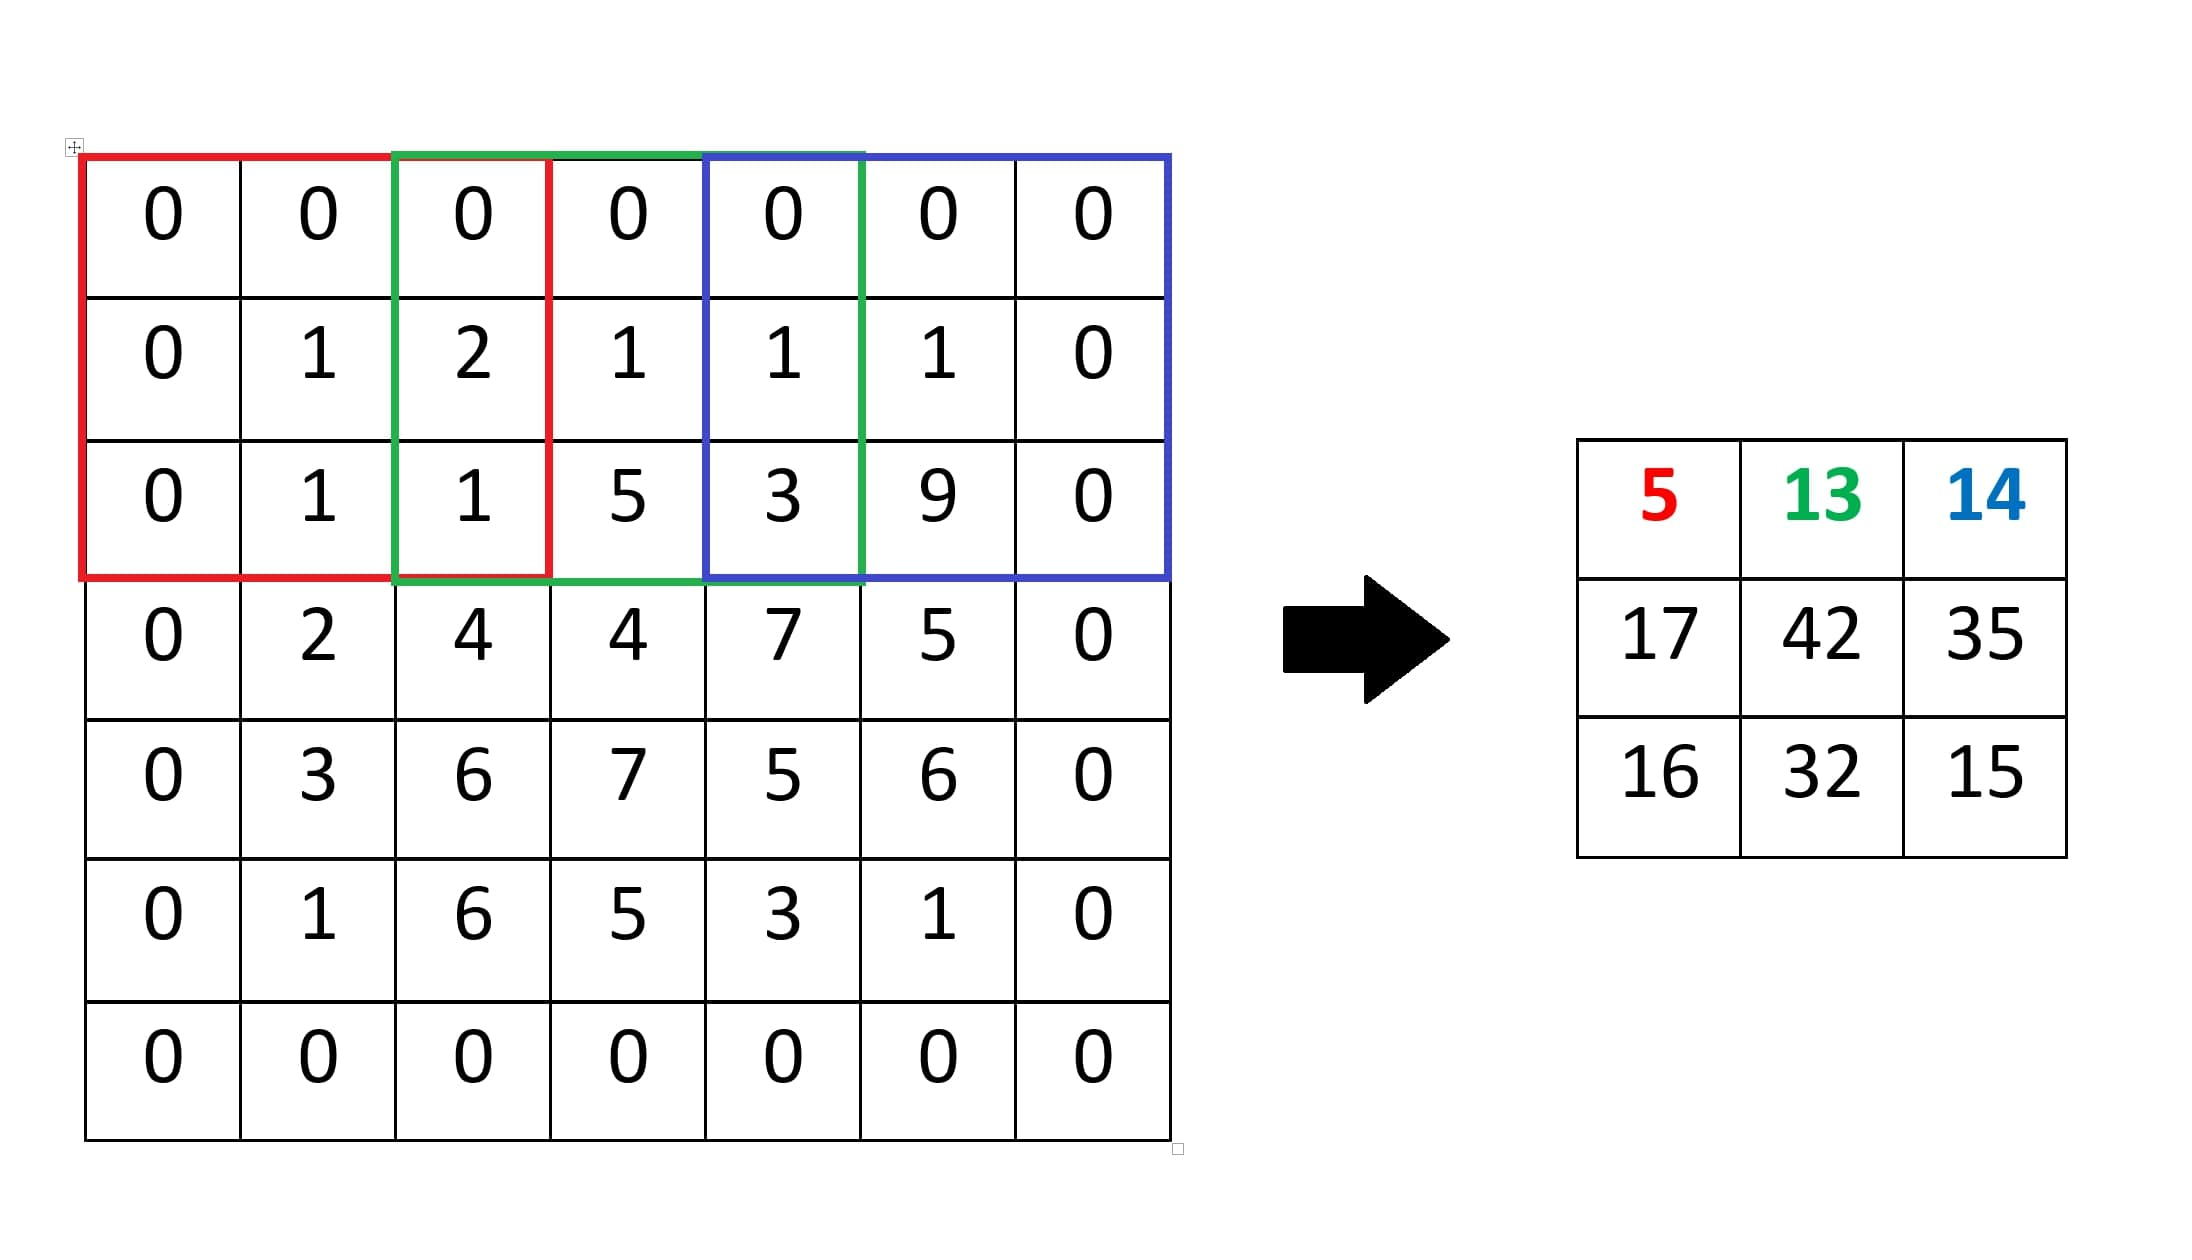
\includegraphics[scale=0.15]{convolution.jpg}
\caption{Convolution eines $7 \times 7$ Bildes mittels $3 \times 3$ Eins-Filter ($w_{i,k} = 1$), Padding = 1 und Stride = 2}
\end{figure}

Jeder Filter erstreckt sich über die gesamte Tiefe des Bildes. Wird also ein $B\times B\times 3$ Filter auf ein $A\times A\times 3$ Bild angewandt, so hat das Ausgabebild die Dimension $C\times C\times 1$ mit $C = \frac{A-B}{stride+1}$. Werden $10$ Filter der Größe $B\times B\times 3$ angewandt, so hat die Ausgabe die Dimension $C\times C\times 10$. Je mehr Filter angewandt werden, desto besser können Muster gelernt werden. Zu große und zu kleine Filter führen zu Over- und zu Underfitting.

\item \textbf{2. ReLU Layer} Diese Schicht übernimmt das Aktivieren der einzelnen Gewichte mit z.B. max(0,x).

\item \textbf{3. Pooling Layer} Diese Schicht reduziert die Ausgabe nach der Filterung und Aktivierung auf wesentliche Merkmale des Bildes und verkleinert die Anzahl der Pixel, die für die Speicherung dieser Merkmale notwendig sind. Zum Einsatz kommt meistens das Max-Pooling. Hierbei wird wie bei der Convolution eine Maske auf das Bild gesetzt. Das Maximum aller Bildwerte, die sich hinter der Maske befinden, ist der Wert des neuen Bildes nach dem Pooling. 

\begin{figure}[H]
\centering
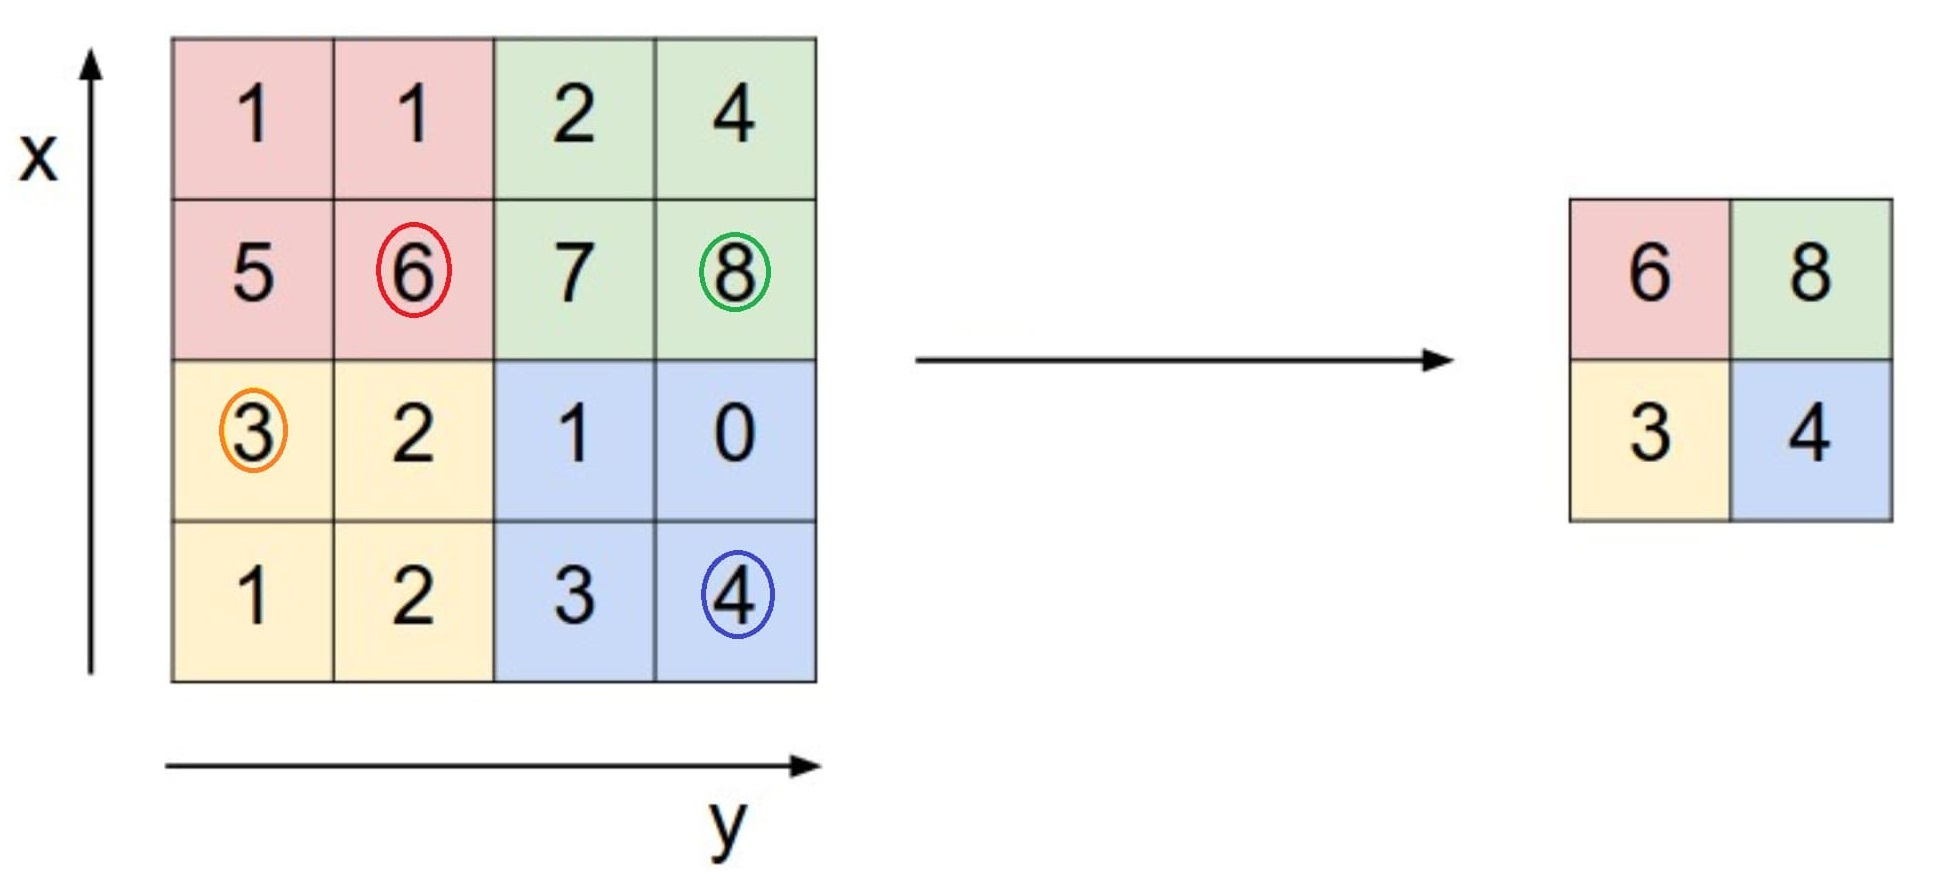
\includegraphics[scale=0.3]{pooling.jpg}
\caption{Pooling mit stride = 2}
\end{figure}

\item \textbf{4. Fully Connected Layer} Diese Neuronen-Schicht soll die Ausgabe nach den oben genannten Schritten interpretierbar machen und auf Klassen-Scores abbilden. Jedes Neuron ist mit jedem aktivierten Gewicht der davor liegenden Schicht verbunden.
\begin{figure}[H]
\centering
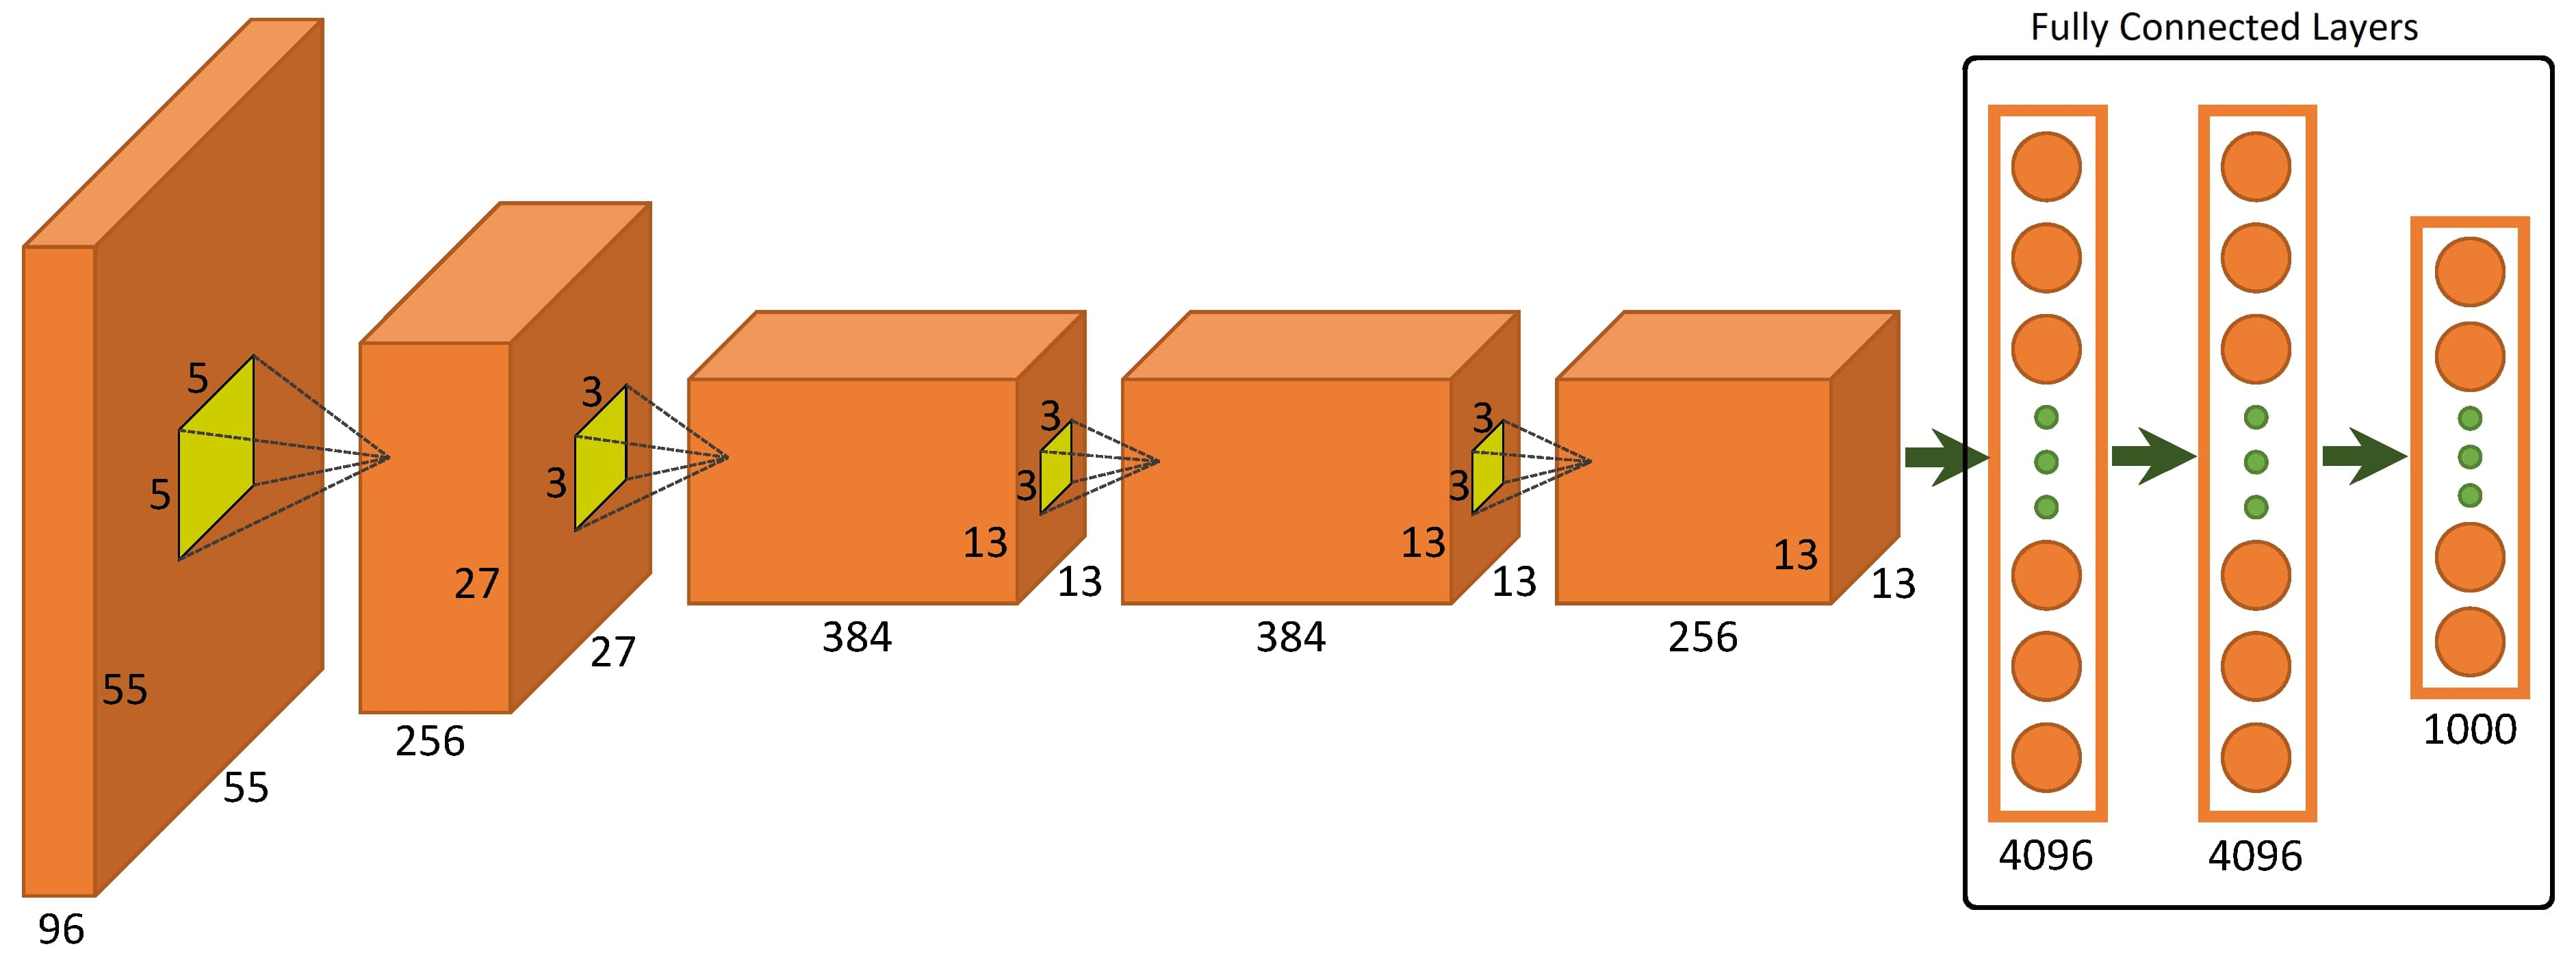
\includegraphics[scale=0.1]{conv-construction.jpg}
\caption{Gewöhnliches Convnet mit Fully Connected Layers zum Schluss}
\end{figure}

\end{itemize}

\begin{figure}[H]
\centering
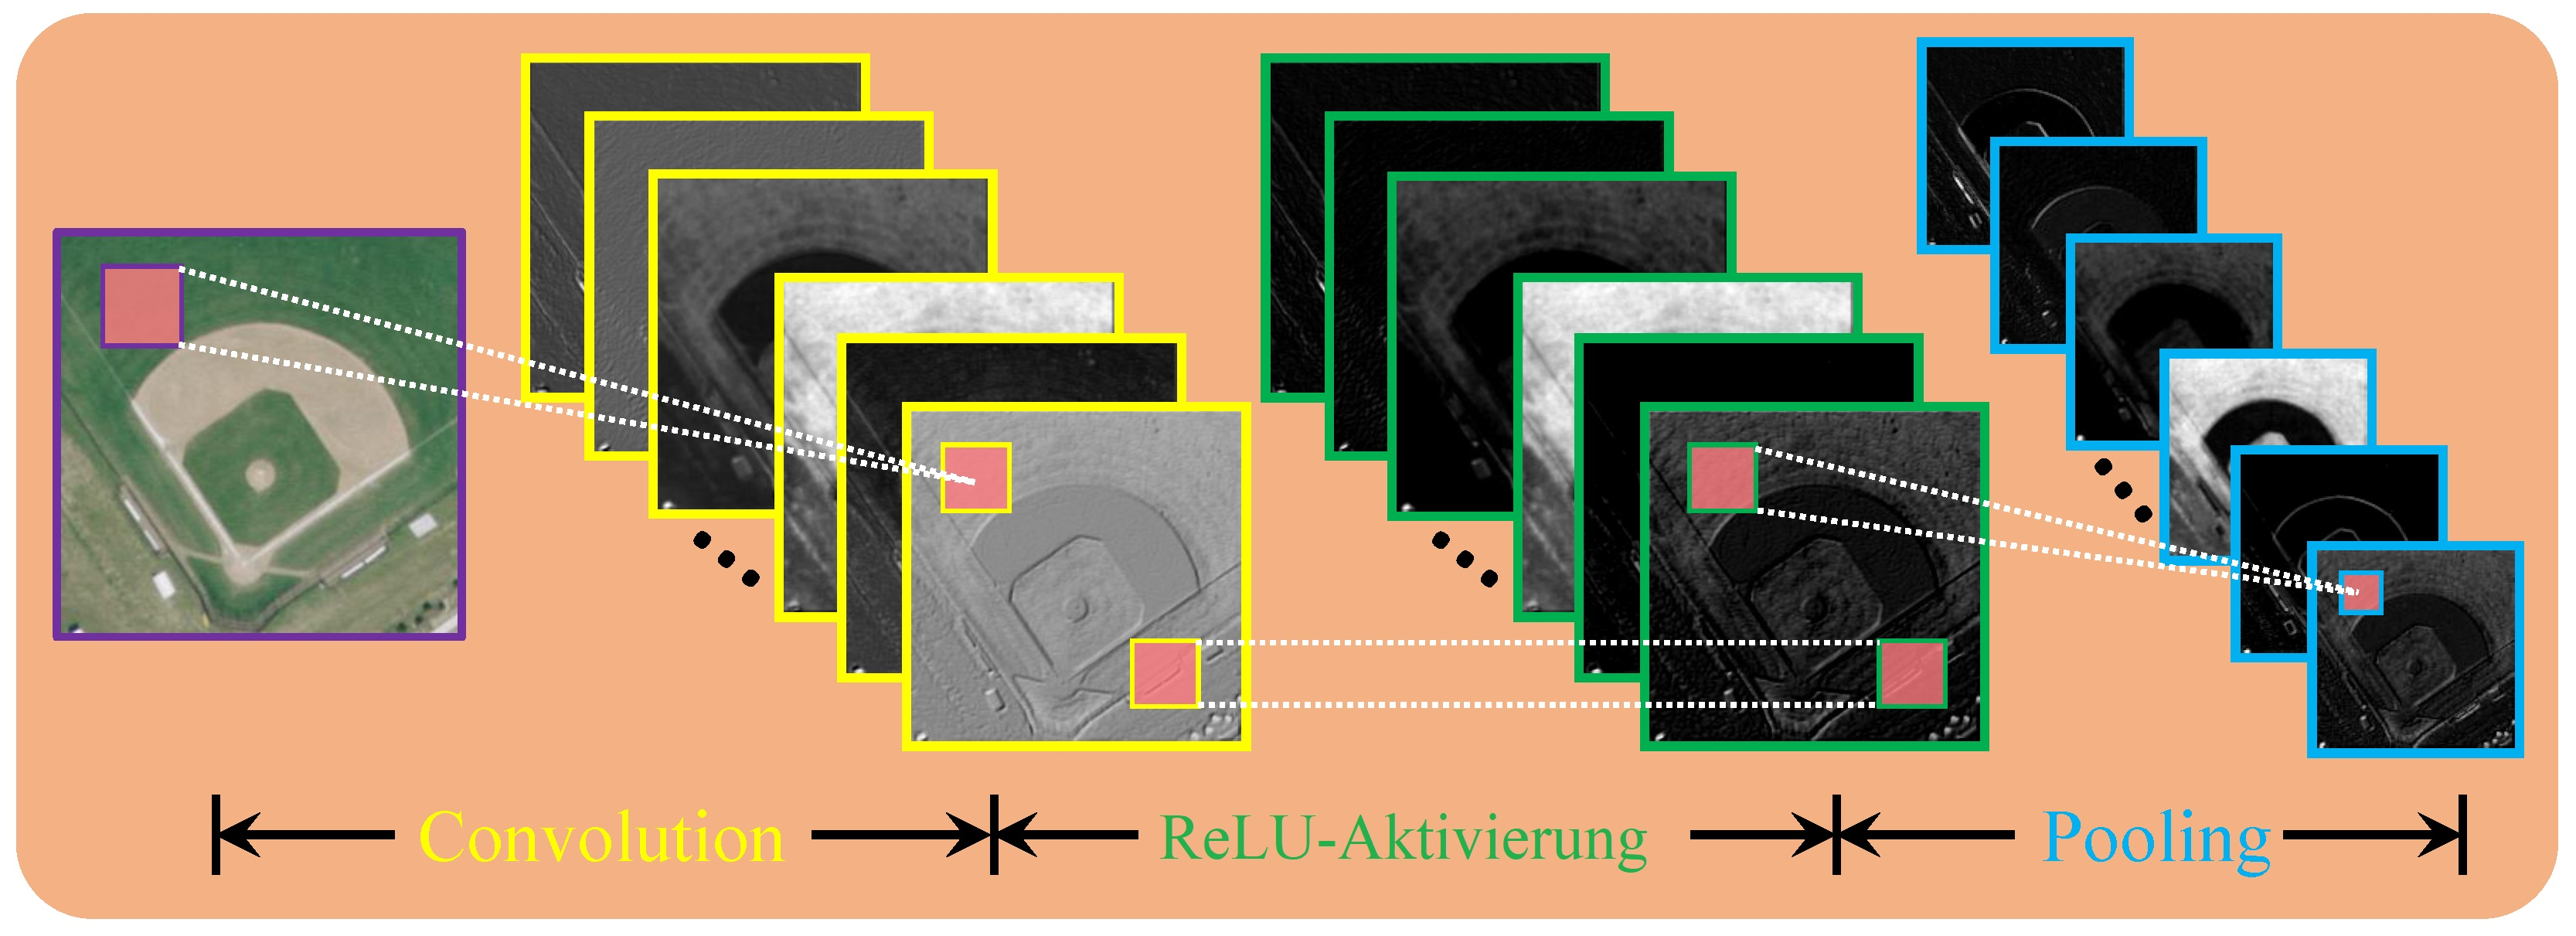
\includegraphics[scale=0.25]{conv-layers.jpg}
\caption{Verbildlichung der Schritte 1-3 durch Anwendung von Convolution auf ein Luftbild\protect\footnotemark}
\end{figure}
\footnotetext{http://www.mdpi.com/2072-4292/7/11/14680/htm}


\subsection{Recurrent Neural Network}
Ein Recurrent Neural Network (RNN) ist ein zeitabhängiges neuronales Netz, mit welchem sich Zustände vorhersagen lassen. So lassen sich mit einem RNN z.B. folgende Probleme Lösen:

\begin{itemize}
\item Image Captioning
\item Sentimentanalyse (Stimmungserkennung im Text Mining)
\item Sprachübersetzung, Textproduktion und Vorhersage von Worten
\item Videoklassifikation
\item Vorhersage von geologischen Aktivitäten
\end{itemize}

Ein Zustand $h_t$ und eine Ausgabe $y_t$ eines RNN zu einem bestimmten Zeitpunkt $t$ berechnet sich wie folgt:

\[h_t = f(W_{xh} x_t + W_{hh} h_{t-1} + b1)\]
\[y_t = g(W_{hy} h_t + b2)\]

Hierbei enthalten die Gewichtsmatrizen $W_{xh}$, $W_{hh}$, $W_{hy}$ die zu lernenden Parameter zwischen Input Layer, Hidden Layer und Output Layer. Die Funktionen $f$ und $g$ sind Nichtlinearitäten.
\\~\\
\textbf{Beispiel:}\\
Ein RNN wird mit einer gegebenen Sequenz ('h' 'e' 'l' 'l' 'o') 
trainiert, sodass es bei der Eingabesequenz x = ('h' 'e' 'l' 'l') die Sequenz ('e' 'l' 'l' 'o') und somit den Buchstaben 'o' korrekt vorhersagt. 
\begin{figure}[H]
\centering
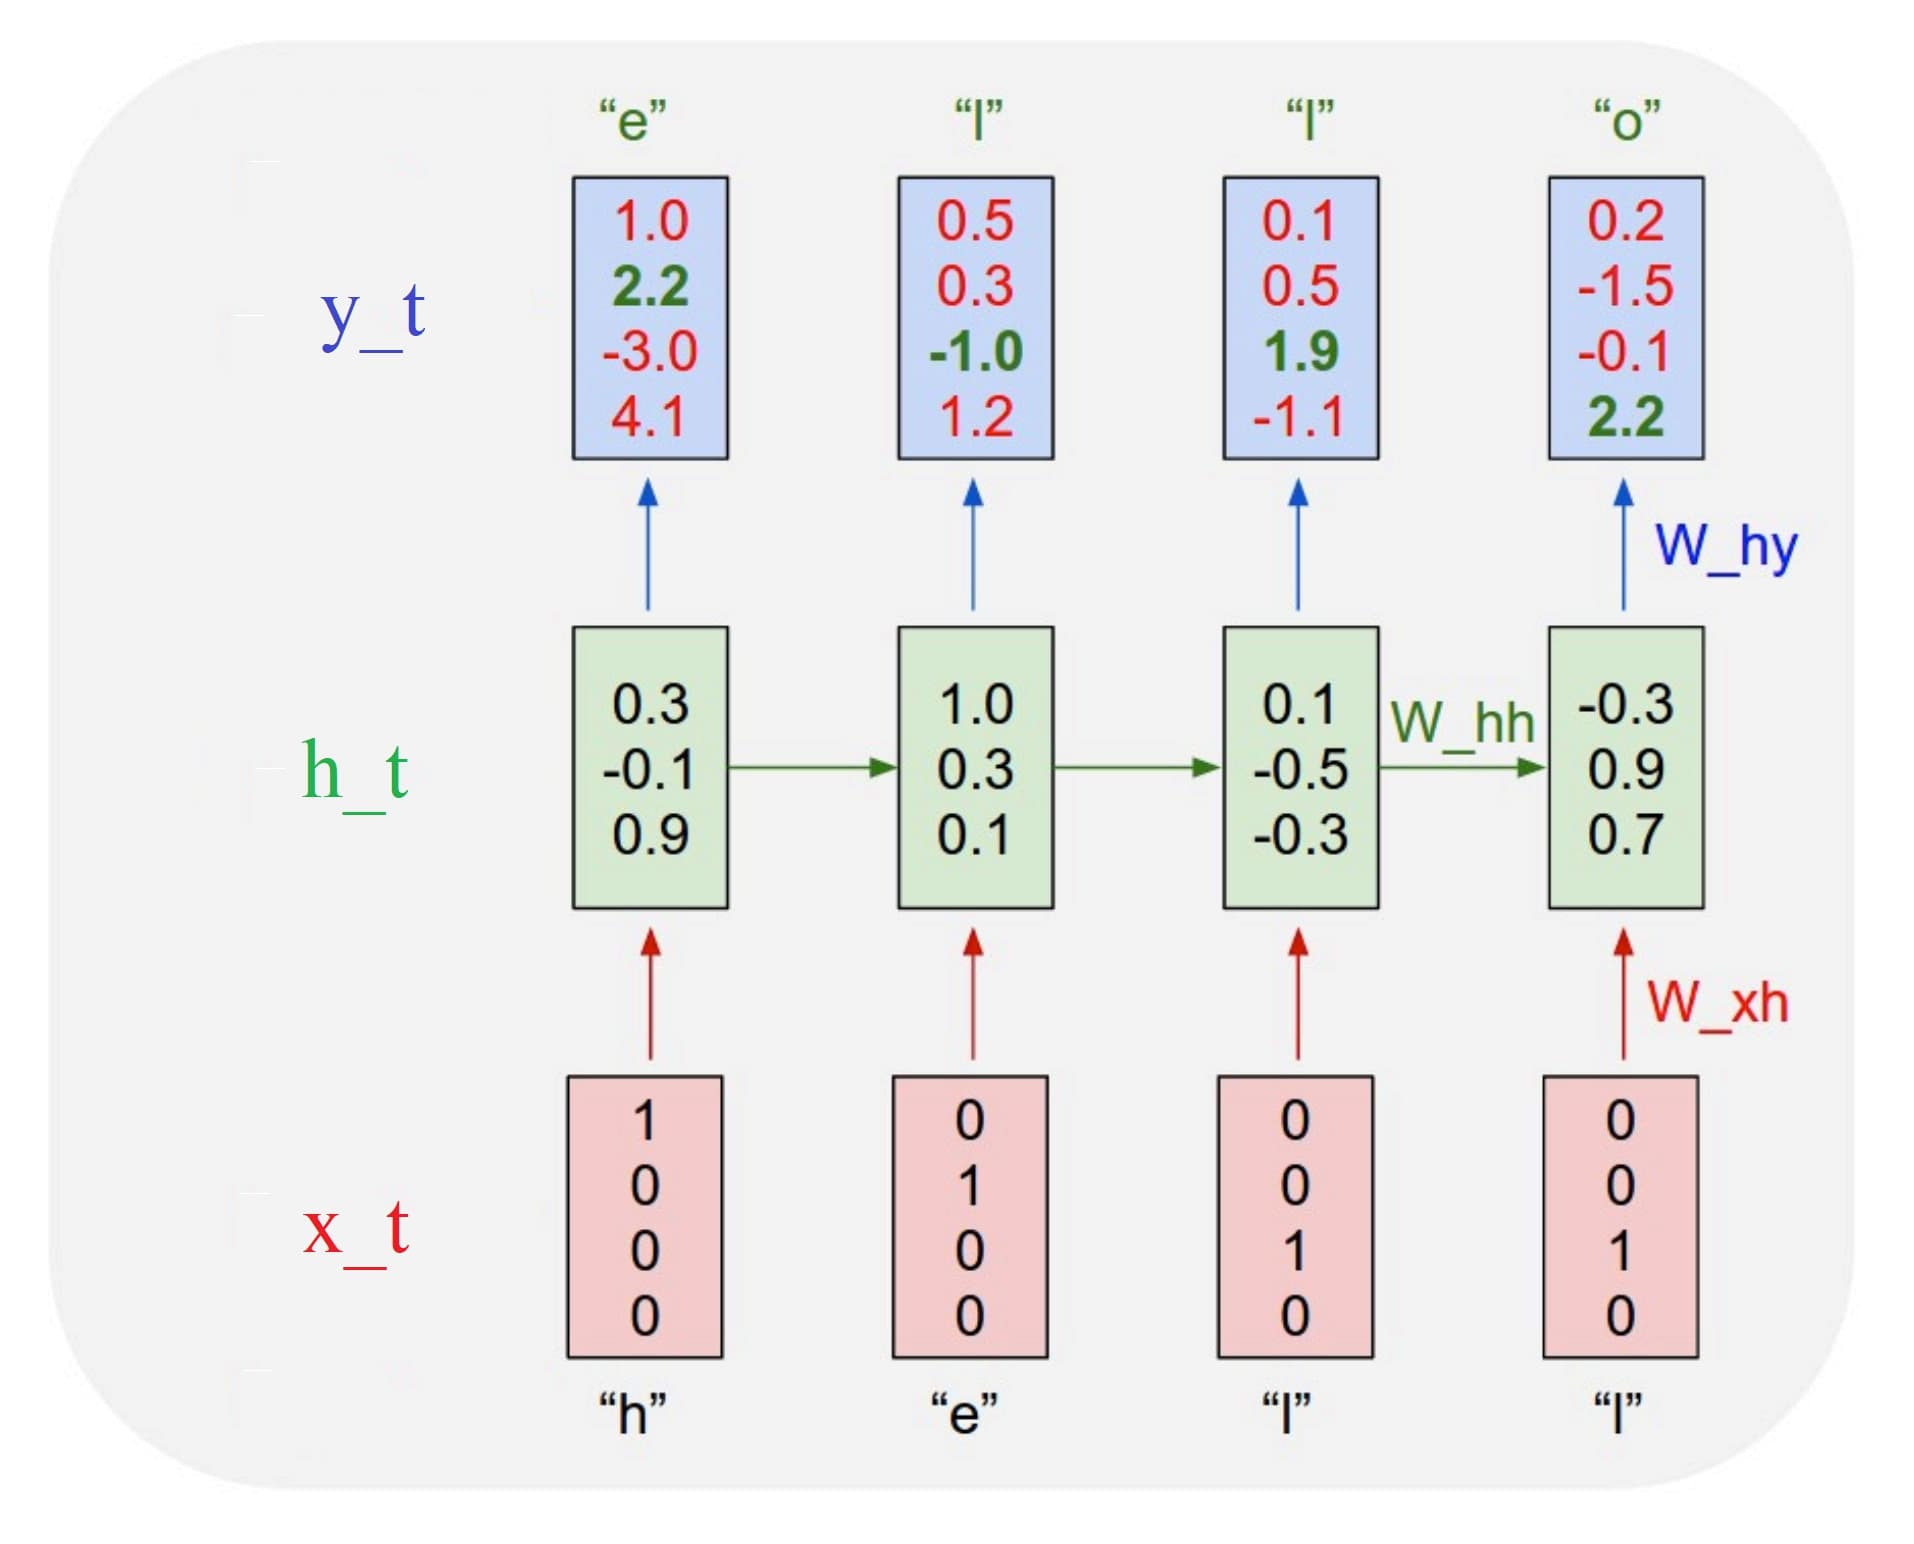
\includegraphics[scale=0.15]{RNN.jpg}
\caption{RNN vervollständigt das Wort \textit{hello}}
\end{figure}

Die Gewichtsmatrix $W_{xh}$ speichert, wie Buchstaben zu Hidden States umgewandelt und inkrementiert werden. $W_{hy}$ lernt, welcher Ausgabebuchstabe zu dem gegebenen Hidden State passt und die Matrix $W_{hh}$ akkumuliert und migriert alle bisherigen Eingaben im zeitlichen Verlauf zu einem gemeinsamen Hidden State.

\newpage
\section{Machine Learning in Geowissenschaften}

\subsection{Herausforderungen und Chancen von Machine Learning  }
\textbf{Einleitung}\\
Die moderne Geowissenschaft steht vor vielen Herausforderungen, wie den Prognosen zu Klimawandel, Luftverschmutzung, Naturkatastrophen, Ressourcenverbrauch oder den Risiken für Erdbeben, Landrutsch und Vulkanausbrüchen. Die Forschung an solchen Problemen macht die interdisziplinäre Arbeit sämtlicher Wissenschaften unumgänglich.
Geowissenschaften haben sich in den letzten Jahrzehnten  zu einer Big-Data Disziplin entwickelt. Angestoßen wurde diese Entwicklung durch technologische Verbesserungen, wie dem Wachstum der Rechenleistung. Aufwändige Simulationen und die Demokratisierung von Datenbeständen, deren öffentliche Verbreitung im Internet und vielseitige Beteiligungsmöglichkeiten trugen ebenfalls dazu bei. Die wachsende Verbreitung großer geowissenschaftlicher Datenbestände ermöglicht ein enormes Potenzial für Maschinelles Lernen\cite{machgeo}.\\

\bigskip

\textbf{Sammeln von Geodaten}\\
Die Erde ist ein komplexes dynamisches System, bestehend aus Litosphäre, Biosphäre, Atmosphäre, Hydrosphäre. Einzelne Bestandteile dieses Systems (z.B. Ozeanschichten oder die Bodenbedeckung) befinden sich in einem ständigen Wandel und interagieren miteinander. Um Daten solcher Phänomene zu erheben, gibt es vor allem zwei Möglichkeiten:
\begin{itemize}
\item Messen mithilfe von Sensoren in/auf Satelliten, Flugzeugen, Ballons, Drohnen, Wetterstationen, Schiffen, Bojen.\newline
Sensorbasierte geowissenschaftliche Beobachtungen sind nicht uniform gerastert und beziehen sich häufig auf irreguläre Zeitintervalle (zum Beispiel schwankt die Position einer Boje mit der Zeit). Sie eignen sich jedoch Hervorragend zum sammeln von Daten wie Oberflächentemperatur, Luftfeuchtigkeit, Reflektionintensität, Chemischer Zusammensetzung der Atmosphäre, Strömungen und Drücke, Emissionen, seismischer Aktivität und der Oberflächengestalt der Erde. Diese Vielfalt an geologischen Eigenschaften erfordert bezüglich eines gegebenen Problems eine individuelle Zusammenstellung von relevanten Datensätzen. Die Datentypen müssen gegebenenfalls konvertiert und die Datenbestände interpoliert werden, um sie besser interpretierbar zu machen.

\item \textbf{Ableiten aus mathematischen Modellen und Simulationen}
Geologische Prozesse, ihre Interaktionen und Änderungen sind auf physikalische Gesetze zurückzuführen. Zum Beispiel sind Bewegungen von Wasser in der Liosphäre auf die Strömungsdynamic zurückzuführen. Ein Nachteil physikalischer Berechnungen auf Grundlage von Modellen für komplexe Systeme ist leider deren Ungenauigkeit. Dennoch eignen sie sich zur näherungsweisen Darstellung des zeitlichen Verlaufes von geophysikalischen Phänomenen. Ein weiterer Vorteil ist, dass Simulationen besonders große Datensätze erzeugen können, wenn Daten für große Zeitintervalle von Interesse sind. Diese ermöglichen dann wiederum eine Datenbasierte Analyse mittels Machine Learning.
\end{itemize}
\bigskip
\textbf{Herausforderungen}
Leider ist die Nützlichkeit von Machine Learning für Knowledge Discovery häufig begrenzt. Geophysikalische Objekte sind häufig nicht klar definiert (keine klar definierten Grenzen) und ändern sich häufig. Daten zu solchen Objekten können ebenfalls unterschiedliche Auflösungen haben, rauschen, unvollständig oder ungenau sein. Auch kann die zeitliche Auflösung aus historischen Gründen stark variieren (z.B. ein Weltkrieg, in dem historische Datensätze zerstört wurden). Auch liegen häufig nicht ausreichend Geländedaten vor. Die Herausforderungen lassen sich in 3 Hauptkategorien unterteilen:

\begin{itemize}
\item \textbf{Eigenschaften Geologischer Prozesse}
\begin{itemize}\item \textbf{Amorphe Grenzen (Wellen, Flüsse, Stürme)} Segmentierungs- und Clusteringverfahren sowie Maßnahmen für Feature-Charakterisierungen sind notwendig.
\item \textbf{Raumzeitliche Struktur}  
Für viele Machine Learning Methoden nimmt man an, dass beobachtete geophysikalische Eigenschaften nicht korrelieren und die erhobenen Daten gleichverteilt sind. Die Realität sieht anders aus. 
Benachbarte Orte sind stark korreliert (Wahrscheinlichkeit für Grasland ist in der Nähe eines Waldes größer als in einer Wüste). Änderungen (Wald => Wüste) bewirken Zustände, die für eine unbestimmbare Zeit persistieren (Die Wüste wird nicht regelmäßig zum Wald und umgekehrt), was auf Klimaveränderungen zurückzuführen ist.
Zwei weit entfernte Orte können ebenfalls stark korrelierte Eigenschaften besitzen (z.B. Temperatur, Druck). Man nennt diese meist meteorologischen Korrelationen Telekonnektionen .
\item \textbf{Hochdimensionalität} Die Erde ist eines der komplexesten bekannten Systeme mit einer extrem großen Anzahl an Variablen, die alle miteinander in sowohl räumlich als auch zeitlich relativ zur Größe der Erde winzigen Skalen miteinander wechselwirken. Für eine Verarbeitung und Speicherung von Daten solcher Systeme ist die Rechenleistung heutiger Computer nicht ausreichend.
\item \textbf{Raumzeitliche Variabilität} Geologische Prozesse können stark schwanken, sowohl in kurzen Zeitintervallen (Jahreszeiten, Tidenhub), in langen Zeitintervallen (Polsprung, Präzession, Klimawandel) als auch räumlich (Gebirgsformationen, Vegetationszonen, Klimazonen). Es ist sehr schwierig ein Modell zu trainieren, dass alle diese Prozesse vereint. Eine lokale und zeitliche Begrenzung der Datensätze ist zwingend erforderlich.
\item Seltene Phänomene - Seltene Ereignisse wie z.B. Vulkanausbrüche, Tsunamis und Erdbeben verfälschen das Modell, da sie nur für ein Training auf viel größeren Zeitskalen geeignet sind. Aus diesem Grund müssen sie erkannt und aus dem Modell herausgerechnet werden. Dies ist nahezu unmöglich, da es hierzu keine ausreichenden Erfahrungswerte gibt.
\end{itemize}

\item \textbf{Sammeln von Geodaten}
\begin{itemize}
\item Daten mit verschiedenen Auflösungen - Beispiel: Zur Beurteilung von Waldbränden müssen Bilder aus Luftaufnahmen und Satellitenbilder miteinander kombiniert werden. Die Flugzeugbilder haben eine höhere räumliche Auflösung, die Satellitenbilder wurden jedoch in regelmäßigen Zeitabständen aufgenommen. Aus diesem Grund müssen Interpolations- oder Upsamplingmethoden entworfen werden, um die beiden Arten von Bildern vergleichbar zu machen.
\item Rauschen, Unvollständigkeit, Ungenauigkeit - Viele Geodatensätze sind unvollständig oder rauschen, weil z.B. Sensoren temporär ausgefallen sind oder unter verschiedenen Wetterbedingungen Messungen durchgeführt haben. Manche Daten sind erst dann interpretierbar, wenn Sie mit einem mathematischen Modell kombiniert werden. Dieses kann die Interpretierbarkeit jedoch ebenfalls beeinflussen.
\end{itemize}

\item \textbf{Mangelhafte Datensätze}
\begin{itemize}
\item \textbf{Kleine Sample-Größe} Viele Datenbestände sind niedrigfrequent und extrem ungenau, wenn sie aus einer Zeit stammen, in welcher es entweder keine oder nur wenige Messinstrumente gab. Auch gibt es Orte, an denen es nur schwer möglich ist (zeitlich hochfrequente) Messungen durchzuführen (Bohrkernanalyse in Antarktis o.ä., Bäume mit ausreichendem Alter für Jahresringe). Eisbohrkerne aus der Antarktis lassen zudem keine Rückschlüsse über die Klimatischen Verhältnisse in anderen Regionen zu. 
\item  \textbf{Mangelhafte gelabelte Geländedaten} Oft liegen Geländedaten in mangelnder Qualität vor. Dies liegt daran, dass sie nur mit Zeit- und Kostenintensiven Maßnahmen zu beschaffen sind. Eine geringe Datenqualität führt zu einem langsamen Trainingsprozesses und zu Unter- oder Überanpassung des Modells, was die Aussagekraft stark einschränkt.
\end{itemize}
Aus beiden oben genannten Gründen müssen Trainingsmodelle entwickelt werden, die mit kleineren Datensätzen zurecht kommen.
\end{itemize}
\bigskip
Maschinelles Lernalgorithmen können dazu beitragen, Geowissenschaftliche Objekte und Ereignisse zu Charakterisieren und somit helfen, das Erdsystem besser zu verstehen. Während traditionelle Ansätze auf handgefertigten Algorithmen basieren, können Machine Learning Algorithmen mit ihrer automatischen Mustererkennung die Berechnungszeit deutlich verkürzen. Eine große Herausforderung stellt die Charakterisierung von physikalisch ungenau definierten Objekten dar. Unsupervised Learning kann dabei helfen, anomalische Objekte aufzuspüren (z.B. Landminen).\\
\bigskip
Ein weiterer großer Vorteil von Machine Learning ist die Erzeugung von Geodaten aus nur schwer beobachtbaren Prozessen (z.B. Methanausstoß und Konzentration in der Atmosphäre). Supervised Learning kann verwendet werden, um Fernerkundungsdaten zu analysieren und daraus Aussagen über das Ökosystem abzuleiten (z.B. Gesundheit der Vegetation oder Wasserqualität). Eine besondere Herausforderung ist dabei die Heterogenität solcher Daten, wie bereits weiter oben beschrieben. Eine mögliche Lösung sind Multi-Task-Learning-Frameworks, welche Datensätze zuerst in homogene Partitionen unterteilen (hierarchisches Clustern), und dann auf jeder dieser Partitionen einzeln trainieren. Dieses Vorgehen ist eine Regularisierungstechnik, welche die Überanpassung des Modells verhindern soll. Folgende Abbildung zeigt die Verbesserung der Genauigkeit der geschätzten Waldbedeckung vier brasilianischer Staaten, wobei die rot markierten Bereiche die Residuen darstellen.
\begin{figure}[H]
\centering
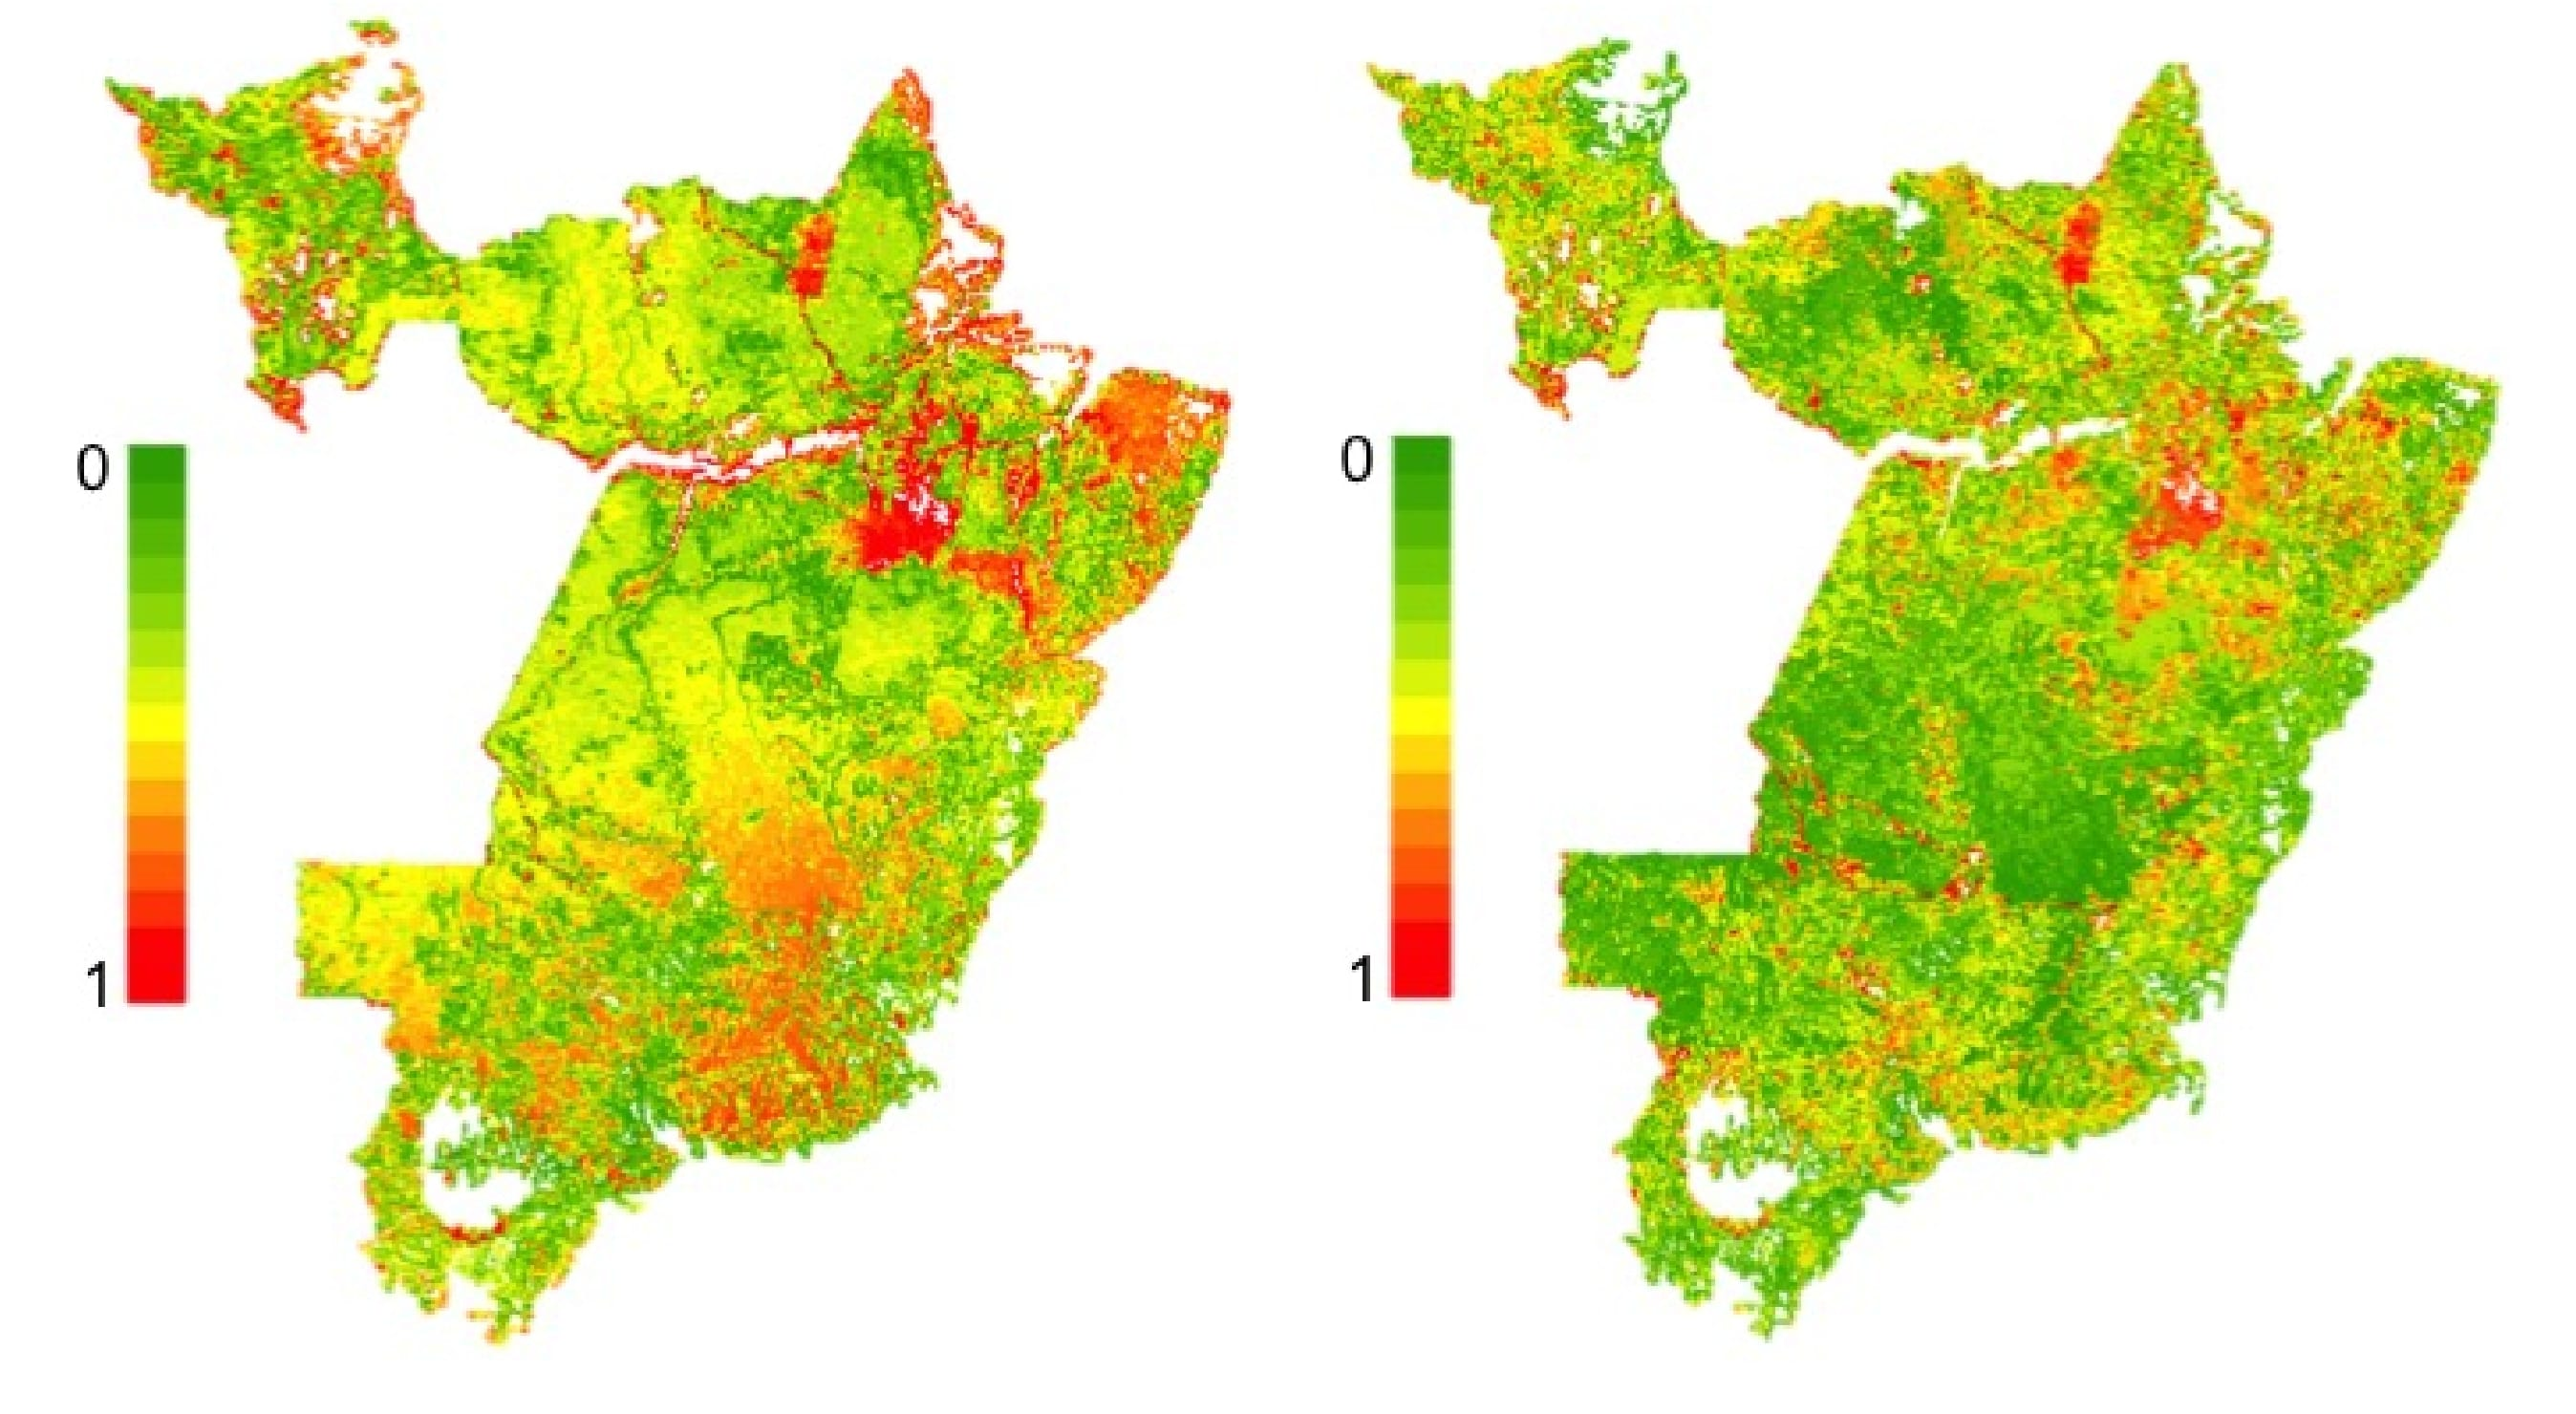
\includegraphics[scale=0.1]{multi-task-learning.jpg}
\caption{Schätzung der Waldbedeckung in Brasilien \protect\footnotemark}
\end{figure}
\footnotetext{A. Karpatne, Z. Jiang, R. R. Vatsavai, S. Shekhar, and V. Kumar,
Monitoring Land-Cover Changes. IEEE Geoscience and Remote
Sensing Magazine, 2016}~\\
\bigskip
\textbf{Nichtstationarität, Heterogenität und Mangeldaten}\\
Zum Umgang mit der Nichtstationarität (= Variable folgt keinem konstanten Wert) von Klimadaten wurden lernende Algorithmen entworfen, welche die Vorhersagen verschiedener Klimamodelle kombinieren. Statt eines Mittelwertes über die Klimamodelle berücksichtigt der selbstlernende Algorithmus zusätzlich  die nichtstationären Dateneigenschaften und erzeugt wesentlich genauerer Vorhersagen.

Heterogene und minderqualitative Daten können mithilfe von \textit{Adaptive Ensemble Learning} und \textit{Label Refinement} besser analysiert werden.

Zur Näherung von Geophysikalischen Variablen mit Daten geringer zeitlicher Auflösung und fehlender Labels können folgende Techniken verwendet werden:
- Regularisierer (für zeitl. Auflösung)
- Semi-Supervised-Learning (fehlende Labels)
- Active Learning (genauere Ergebnisse für Berechnungsprobleme)
- Unsupervised Learning (bessere Näherung für geophysikalische Größen und Kartierung von Flächenänderungen durch z.B. Insektensterben, Waldabholzung und Ackerlandumwandlung)\\

\bigskip
\textbf{Techniken für Langzeitvorhersagen}\\
Eine Möglichkeit für Langzeitvorhersagen war bisher die Verwendung von physikalischen Modellsimulationen. Diese können jedoch auch als Zeitreihen-Regressions-Problem aufgefasst werden. Mögliche Methoden zur Lösung solcher Probleme sind z.B.:
\begin{itemize}
\item Exponential Smoothing Techniques
\item Autoregressive Integrated Moving Average (ARIMA) Modelle
\item State-space Modelle 
\item Hidden Markov Modelle
\item Kalman Filter
\end{itemize}
Transfer Learning - Ein zu trainierendes Modell für ein Problem mit wenig Daten soll mithilfe eines zuvor trainierten Modells mit vielen Daten das Problem besser lösen.\\

\bigskip
\textbf{Relationen und Kausalität}\\
Geophysikalische Zusammenhänge (z.B. Telekonnektionen und Dipole), sollen sich mithilfe datenbasierter Ansätze besser verstehen lassen. Man erhofft sich durch sie die Entdeckung neuer Korrelationsmuster.
Darüber hinaus können graphenbasierte Repräsentationen von Klimadaten mithilfe von Clustering und Mustererkennung besser analysiert werden.
\bigskip
Eine besondere Herausforderung bei der Korellationserkennung ist der besonders große Suchraum mit all seinen raumzeitlichen Objekten und dynamischen, rauschenden und unvollständigen Geodaten. Es herrscht ein großer Bedarf an neuen Ansätzen, die gleichzeitig sowohl Zusammenhänge als auch die dazugehörigen interagierenden Objekte erkennen.\\
Ursache-Wirkungszusammenhänge zu entdecken ist eine weitere wichtige Aufgabe in den Geowissenschaften. Ein häufig eingesetztes Tool für die Analyse von solchen kausalen Zusammenhängen ist die multivariate Grangeranalyse mittels Vektorautoregression. Auf diese Weise können z.B. Sturmverläufe vorhergesagt werden. Weitere kaum erforschte Mgölichkeiten sind das Reinforcement Learning und stoastische Anstze der dynamischen Programmierung zur Lösung von Entscheidungsproblemen.
\\ \bigskip
\textbf{Deep Learning}\\
Neuronale Netze haben die Eigenschaft, komplexe Features mithilfe der Verknüpfung weniger komplexer Features darzustellen. In Kombination mit dem Training großer Datensätze und der Fähigkeit, Fehler an den Nodes der Hidden-Layers zu minimieren, haben neuronale Netze weite Felder im Bereich Machine Learning revolutioniert. Darunter auch  Supervised, Semi-Supervised, und Reinforcement Learning. Häufig werden neuronale Netze eingesetzt, wenn es schwierig ist, mittels handgeschriebener Algorithmen die wirklich relevanten Features aus einem komplexen Datensatz (wie es auch Geodatensätze sind) zu extrahieren. Geophysikalische Fragestellungen und Probleme haben viele Ähnlichkeiten zu den Themen, die im Bereich Computer Vision und Spracherkennung behandelt werden. \\
\bigskip
Während man ein Convolutional Neural Network einsetzt, um auf einem Bild eine Katze zu klassifizieren, kann man dieses auch verwenden, um Wetterphänomene wie Tornados auf Satellitenbildern zu erkennen. \\ \bigskip
Rekurrente Neuronale Netze mit Longshort-Term-Memory Zellen (LSTM) können z.B. genutzt werden, um zeitlich dynamische Plantagen mittels Fernerkundungsdaten kartografieren. RNNs besitzen die Eigenschaft besitzen, zeitlich vergangene Information zu speichern und in zukünftige Vorhersagen mit einzubeziehen. Aus diesem Grund eignen Sie sich zur Vorhersage von geologischen Ereignissen mit angemessener Vorlaufzeit.\\
\bigskip
Deep Learning kann bisher nur bei ausreichend gelabelten Daten zum Einsatz kommen. Aus diesem Grund herrscht hier ein Bedarf an neuen Verfahren, die mit nur wenigen Daten zurechtkommen.\\
\bigskip
\textbf{Fazit}\\
Die Forschung der letzten Jahre hat gezeigt, dass weder ein reiner Datenansatz noch ein reiner mathematischer Modellansatz ausreichend ist, um Knowledge Discovery effizient betreiben zu können. Aus diesem Grund sollten zukünftige physikalische Erkenntnisse möglichst früh und tief in Datenwissenschaftlichen Ansätze einbezogen werden. Auf diese Weise lässt sich auch die Wahrscheinlichkeit für Overfitting reduzieren, vor allem bei mangelnden Trainingsdaten.

%----------------------------------------------------------------------------------------
%	CHAPTER 4
%----------------------------------------------------------------------------------------

\chapter{Clusteringverfahren}
~
\section{Definition und Anwendungszweck}
Ziel des Data Mining Prozesses ist es, Muster in Datenbanken zu erkennen und diese in Form von Wissen aufzubereiten. Im Falle des Clusterings werden Datenpunkte in Gruppen (Cluster) eingeteilt, sodass Daten mit ähnlichen Eigenschaften dem gleichen Cluster und Daten mit unterschiedlichen Eigenschaften verschiedenen Clustern zugeordnet werden. Im Bezug auf Geodaten wären zum Beispiel alle Punkte mit Farbwerten dunkelblau dem Cluster Wasser zugeordnet und alle Daten mit grüner Farbe dem Cluster Vegetation. Auf diese Weise lassen sich topologische Grenzen finden. Eine andere Möglichkeit bietet die gewichtete n-dimensionale Clusteranalyse. Sie ermöglicht die Zuordnung komplexer Daten zu komplexen Klassen. Wurde nach der numerischen Diskretisierung eines Objekts eine hohe Anzahl an Eigenschaften gefunden, so müssen Clusteringverfahren angewandt werden, die unterschiedlich dichte Cluster unterschiedlichster Form erkennen können. Unter Umständen müssen die Daten mittels Hauptkomponentenanalyse auf Unterräume transformiert werden oder die Relevanz und Unabhängigkeit einzelner Attribute mittels Entropieanalyse bestimmt werden. Ein Beispiel hierfür ist die Analyse von Spektralklassen des von Geoobjekten reflektierten Lichts. Da das Reflektionsverhalten vieler Objekte für jeden Wellenlängenbereich charakteristisch ist, kann mittels 7D-Clustering (dem Clustering nach Einteilung der Wellenlängen in 7 Bereiche, auch Spektralkanäle genannt) bestimmt werden, um welches Objekt es sich handelt, oder wie eine Landfläche genutzt wird. \newpage
\begin{figure}[H]
\centering
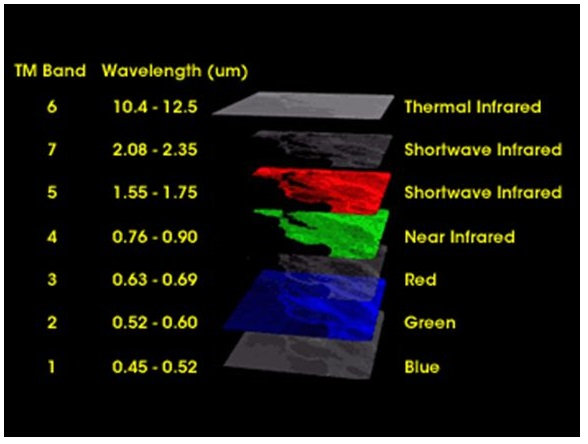
\includegraphics[scale=0.55]{spektral.jpg}
\caption{Landsat Spektralklassen \protect\footnotemark}
\end{figure}
\footnotetext{\url{https://player.slideplayer.org/3/1324211}}
Zu neuronalen Netzwerken, deren Funktionsweise nach dem Trainingsprozess nicht mehr mathematisch nachvollzogen werden kann, bieten Clusteringverfahren eine konkrete, statistische Alternative. Wird ein neuronales Netzwerk hinsichtlich einer Aufgabe angepasst, so ist eine Verbesserung nur über das Ausprobieren verschiedener Architekturen und Parameter verifizierbar. Optimierungen an Clusteringverfahren können jedoch meist als Anpassung einer Optimierungsfunktion formal mathematisch nachvollzogen werden.

\begin{figure}[H]
\centering
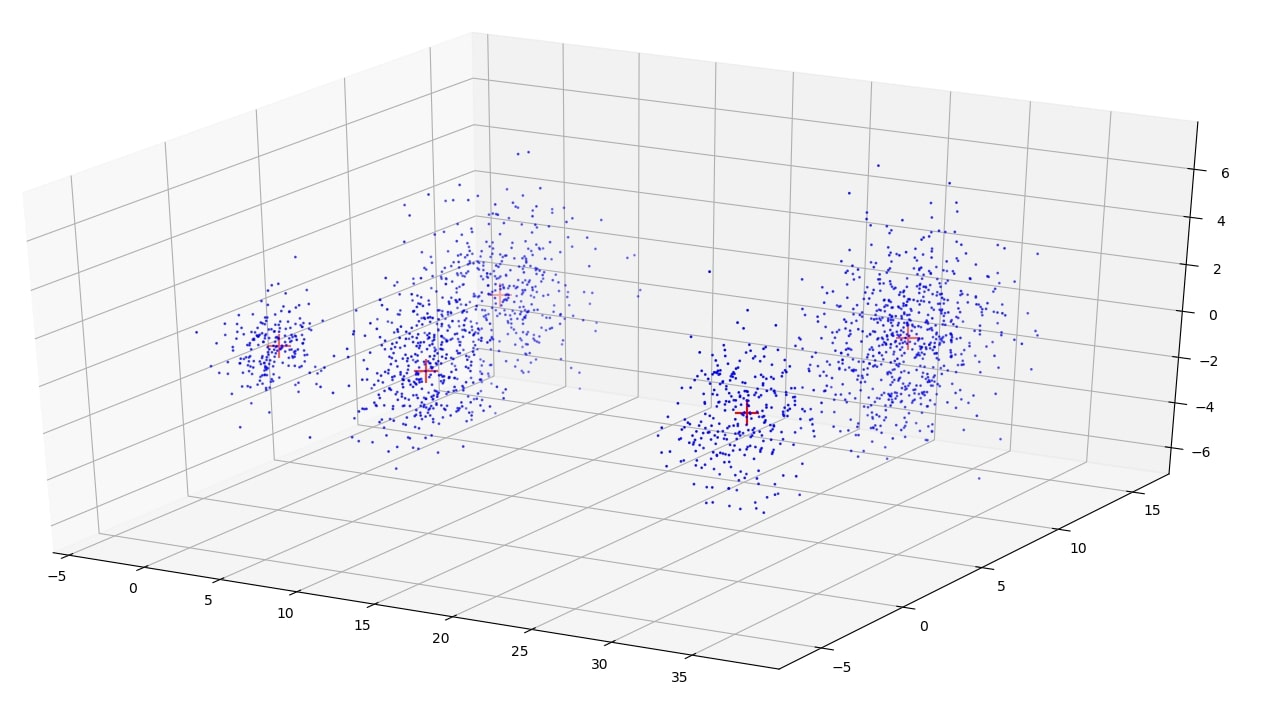
\includegraphics[scale=0.3]{3dcluster.jpg}
\caption{Geclusterter Datensatz: Jedes Datum (blaue Punkte) hat 3 Attribute. Jedes Kreuz ist das Zentrum eines gefundenen Clusters. Die optimale Clusteranzahl wurde mithilfe von Cluster Validity Indizes bestimmt.}\label{cluster}
\end{figure}

Man unterscheidet zwischen harten (crisp) und weichen (fuzzy) Clusteringverfahren. Harte Methoden ordnen jedes Datum einer Datenbank einem Cluster eindeutig zu. Häufig kollidiert dieser Ansatz mit dem intuitiven Verständnis eines Menschen. Beispielsweise kann nicht gesagt werden, dass ein 49-jähriger Mensch jung ist und ein 50-Jähriger alt. Der Übergang von jung nach alt ist fließend. Aus diesem Grund gibt es weiche Methoden, die für jedes Datum einen Grad der Zuordnung zu jedem Cluster errechnen. Beispielsweise ist ein 70-Jähriger zu $80\%$ alt und zu $20\%$ jung. Die Summe der Zuordnungsgrade beträgt meistens $100\%$.
\\
\subsection{Die fünf Hauptschritte des Datenclustering}
Der Prozess des Clusterings ist wie beim Data Mining in Hauptschritte unterteilt\cite{csteps}. Sie lauten:
\begin{itemize}
\item \textbf{Feature Extraction} Seien $n$ Objekte ${o_1, o_2, \dots, o_n}$ gegeben. Im ersten Schritt werden diejenigen Features extrahiert, welche die Menge der Objekte am besten beschreiben. Formal lassen sich die Objekte durch die Menge folgender Feature-Vektoren ausdrücken: $$S =  p_1, p_2, p_3, \dots, p_n  \forall p_i \in R^m$$
\item \textbf{Aufstellen der Ähnlichkeitsmatrix} Die Ähnlichkeitsmatrix $P(S)$ der Dimension $C \times n$ repräsentiert ein Clustering in $C$-viele Cluster, wobei jeder Eintrag $u_{ij}, \forall i=1, \dots, n$ und $j=1, \dots, C$ dem Grad der Zugehörigkeit des $i$-ten Objekts zum $j$-ten Cluster entspricht.
\item \textbf{Berechnung der Gruppierungen} Anwenden eines harten oder weichen Clusteringalgorithmus.
\item \textbf{Datenabstraktion} Finden einer anschaulichen Repräsentation der Clusteringergebnisse, meistens auf Basis der Clusterzentroide.
\item \textbf{Evaluation der Ergebnisse} Wie gut ist das Clustering im Vergleich zu anderen Algorithmen? Hat der Algorithmus Cluster gefunden, die gar nicht existieren? Wie ist die Clustertendenz zu bewerten, d.h. gibt es bevorzugte oder benachteiligte Cluster? Schneidet das Clustering für andere Werte $C$ besser ab?
\end{itemize}

\section{Crisp Clustering}

\subsection{Partitionierende Verfahren und ihre Nachteile}
Einem partitionierenden Clusteringalgorithmus wird die feste Anzahl $k$ an Clustern und die Kostenfunktion übergeben, welche für eine optimale Zuordnung einen kleinen Wert zurück gibt.
\subsubsection{Clustering durch Varianzminimierung}
Das einfachste Verfahren basiert auf der Idee, dass die Zuordnung genau dann optimal ist, wenn die Summe der Abstände zwischen Datenpunkten und ihren sogenannten Clusterrepräsentanten möglichst klein wird. Ein Clusterrepräsentant $\mu_{C_i}$ eines Clusters $C_i$ ist der Mittelwert aller Punkte $p = (x_1,\dots,x_d)$ (Dimensionalität $d$ ist die Anzahl der Attribute von $p$), die $C_i$ zugeordnet wurden. Zu Beginn des Algorithmus werden die Clusterprototypen (initiale Repräsentanten) entweder zufällig initialisiert oder auf Basis einer Wahrscheinlichkeitsfunktion so gewählt, dass sie möglichst weit voneinander entfernt sind (k-means++\cite{kmplus}). Dies reduziert die Anzahl der Iterationen bei Optimierung der Kostenfunktion. Anschließend wird jeder Punkt dem Cluster zugeordnet, dessen Repräsentant den kleinsten Abstand zu diesem Punkt hat $(1)$. Auf Basis dieser Zuordnung werden die Repräsentanten erneut berechnet $(2)$. Dabei wird die Kostenfunktion für das gesamte Clustering berücksichtigt:

$$\sum_{i=1}^{k}\sum_{p \in C_i}^{} dist(p,\mu_{C_i})^2$$

Die Distanzfunktion hängt von der Dimensionalität des Datensatzes ab. Die Neuberechnung von Zuordnung $(1)$ und Repräsentanten $(2)$ wird solange wiederholt, bis keine signifikante Änderung mehr auftritt.

\subsubsection{k-means}

Eine beschleunigte Version der Varianzminimierung ist der \textbf{k-means-Algorithmus} \cite{forgy}. Wenn ein Datenpunkt $p$ von Cluster $C_1$ seine Zugehörigkeit an den Cluster $C_2$ verliert, dann wird nicht auf die restlichen Punkte bei der Neuzuordnung gewartet. Stattdessen werden die Clusterzentroide der betreffenden Cluster $C_1$ und $C_2$ wie folgt sofort aktualisiert:
$$\mu_j^{' C_1} = \frac{1}{|C_1|-1}\cdot(|C_1|\cdot \mu_j^{C_1} - x_j^p)$$ und $$\mu_j^{' C_2} = \frac{1}{|C_1|+1}\cdot(|C_2|\cdot \mu_j^{C_2} + x_j^p)$$ 

\begin{figure}[H]
\centering
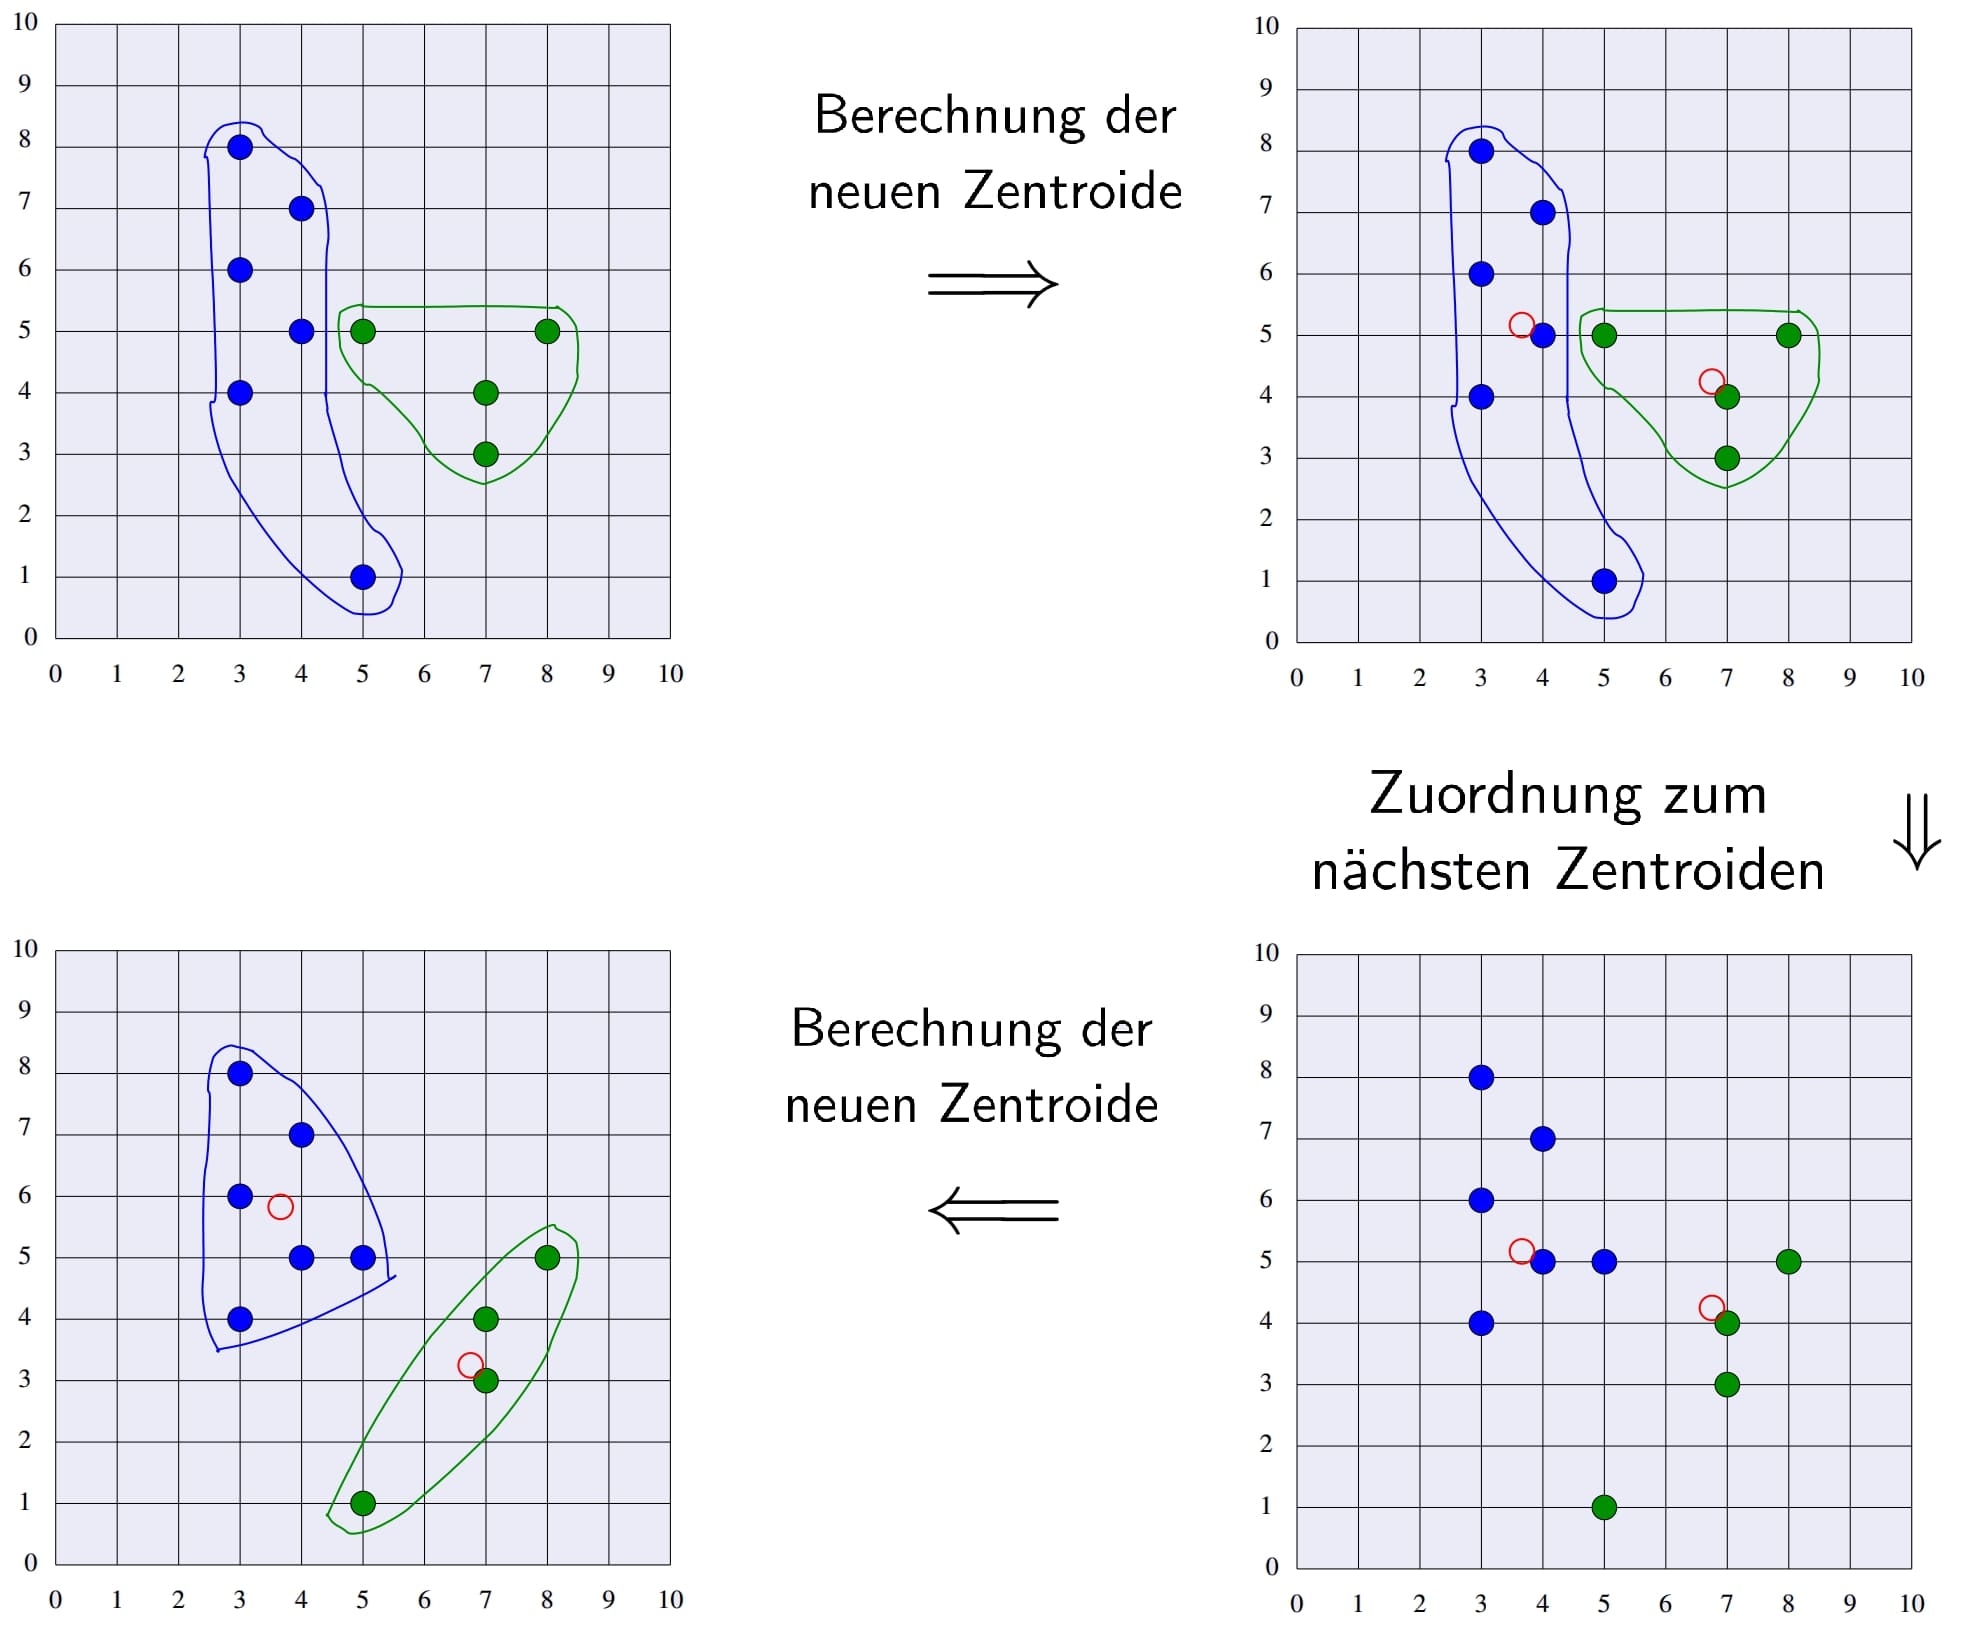
\includegraphics[scale=0.17]{kmeans.jpg}
\caption{Visualisierung des Ablaufs der beiden alternierenden Schritte}\label{cluster}
\end{figure}

Leider erkennt der k-means-Algorithmus weder Cluster unterschiedlicher Dichte, noch unterschiedlicher Form. Auch werden sich überlappende Cluster nicht erkannt. Zudem ist die Qualität des Endergebnisses stark von der initialen Wahl der Clusterprototypen abhängig.

\subsubsection{EM-Algorithmus}
Ein anderer Ansatz der alternierenden Optimierung ist die Erwartungsmaximierung \cite{emalg}. Ihr Vorteil ist, dass auch unterschiedlich geformte und dichte Cluster berücksichtigt werden können. Dabei wird jeder Cluster durch eine Wahrscheinlichkeitsverteilung beschrieben, welche aus der Erzeugung aller Datenpunkte eines Clusters $C$ mittels Kovarianzmatrix $\sum_C$ der Dimension $d \times d$ resultiert. Wie bei der Varianzminimierung bezeichnet $\mu_C$ auch hier den Mittelpunkt aller Daten, die dem Cluster $C$ zugeordnet wurden. Die Wahrscheinlichkeit, mit der bei einer einzigen Normalverteilung $C$ das Datum $x$ erzeugt wurde, beträgt:

$$P(x|C) = \frac{1}{\sqrt{(2\cdot \pi)^d \cdot |\sum_C|}} \cdot e^{-\frac{1}{2}(x - \mu_C)^{\top} \cdot \left(\sum_C\right)^{-1}(x - \mu_C)}$$ 

Da es mehrere Cluster gibt und alle den Punkt $x$ mit einer unterschiedlichen Wahrscheinlichkeit erzeugen, muss die Notation der bedingten Wahrscheinlichkeit erfolgen. Die Wahrscheinlichkeitsdichte eines Clusters bezüglich $x$ lautet $P(x|C_i)$. Sind alle Cluster gaußverteilt, so kann die Gesamtdichte für den Punkt $x$ berechnet werden: $$P(x) = \sum_{i=1}^k W_i \cdot P(x|C_i)$$ 
Wobei $W_i$ der relative Anteil der Datenpunkte ist, die zu Cluster $C_i$ gehören, was der Gesamtwahrscheinlichkeit des Clusters $C_i$ entspricht. Der Satz von Bayes ($P(A|B) = \frac{P(B|A)\cdot P(A)}{P(B)}$) ermöglicht nun die Berechnung der Wahrscheinlichkeit, mit der $x$ zum Cluster $C_i$ gehört:
$$P(C_i|x) = W_i \cdot \frac{P(x|C_i)}{P(x)}$$

Durch die alternierende Berechnung von Zugehörigkeiten $P(C_i|x)$ und Schätzung neuer Verteilungsparameter $\mu_C$, $\sum_C$ und $W_i$ kann das Gütemaß des Clusterings maximiert werden. Es lautet:
$$E(M) = log\left(\prod_{x \in D} P(x)\right)$$

Wobei $M$ die Menge aller Cluster ist: $M = \{C_1, \dots, C_k\}$. Die Optimierung wird abgebrochen, wenn $E(M)-E(M')<\epsilon$, das Gütemaß also nicht mehr in ausreichendem Maße kleiner wird.

\subsection{Silhouettenkoeffizient - Wahl der Clusteranzahl}
Beide vorgestellten Varianten haben die Eigenschaft, das Gütemaß für größere Werte des Parameters $k$ immer weiter zu verbessern. Das Optimum wird erreicht, wenn jedes Datenobjekt genau einen Cluster darstellt, dessen Repräsentant das Datum selbst ist. Um dies zu vermeiden, braucht es ein Gütemaß, welches das Clustering unabhängig von der gewählten Clusteranzahl bewertet. Dieses Gütemaß ist der Silhouettenkoeffizient \cite{silh}.\\
Sei $dist(o,C_i)$ der Abstand eines Punktes $o$ von Cluster $C_i$, also der gemittelte Abstand zwischen $o$ und allen Punkten im Cluster $C_i$. Sei $a(o)$ der Abstand von $o$ zum Cluster, dem $o$ zugeordnet ist und $b(o)$ der Abstand zwischen $o$ und dem nächstgelegenen Cluster (nicht der Cluster, der in $a(o)$ betrachtet wird).
Dann ist die Silhouette eines Objekts $o$:
\begin{equation}
   s(o) =
   \begin{cases}
     0 & \text{wenn } a(o) = 0\\
     \frac{b(o) - a(o)}{max\{a(o), b(o)\}} & \text{sonst} \\
   \end{cases}
\end{equation}

Ist der Wert $s(o) = 1$, dann wurde $o$ seinem Cluster korrekt zugeordnet, ist $s(o) = -1$, dann ist die Zuordnung sehr schlecht.

Der Silhouettenkoeffizient ist dann die durchschnittliche Silhouette aller Datenobjekte aller Cluster im Clustering $C_M = \{C_1, \dots, C_k\}$:
$$s(C_M) = \frac{\sum\limits_{C \in C_M} \sum\limits_{o \in C} s(o)} {|O|}$$

Der Koeffizient nimmt Werte zwischen $0$ und $1$ an, wobei Werte über $0.75$ darauf hindeuten, dass eine sehr gute Zuordnung gefunden wurde. Werte unter $0.25$ deuten auf ein unbrauchbares Clustering hin.

Die optimale Clusteranzahl $k$ kann jetzt bestimmt werden, indem der Silhouettenkoeffizient für verschiedene Clusterings $k = 2, \dots, n-1$ berechnet wird und dann der Wert $k$ ausgewählt wird, für den der Koeffizient den höchsten Wert hat.


\subsection{Dichtebasiertes Clustering (OPTICS)}
Einer der bedeutendsten Clusteringalgorithmen ist das dichtebasierte DBSCAN-Verfahren. Es ist neben seiner Abwandlungen und Optimierungen (OPTICS und HDBSCAN) in vielen Geoinformationssystemen, wie z.B. arcGIS implementiert\footnote{http://pro.arcgis.com/de/pro-app/tool-reference/spatial-statistics/densitybasedclustering.htm}. 

DBSCAN nimmt an, dass Cluster Punktregionen mit höherer Dichte sind, die durch Regionen mit geringerer Dichte (Noise) voneinander getrennt werden. Es kann ausschließlich Cluster desselben Dichteniveaus erkennen. Seine Optimierung OPTICS, welches zu den hierarchischen, dichtebasierten Clusteringverfahren gehört, kann dagegen auch unterschiedlich dichte Cluster und Subcluster erkennen.

\begin{figure}[H]
\centering
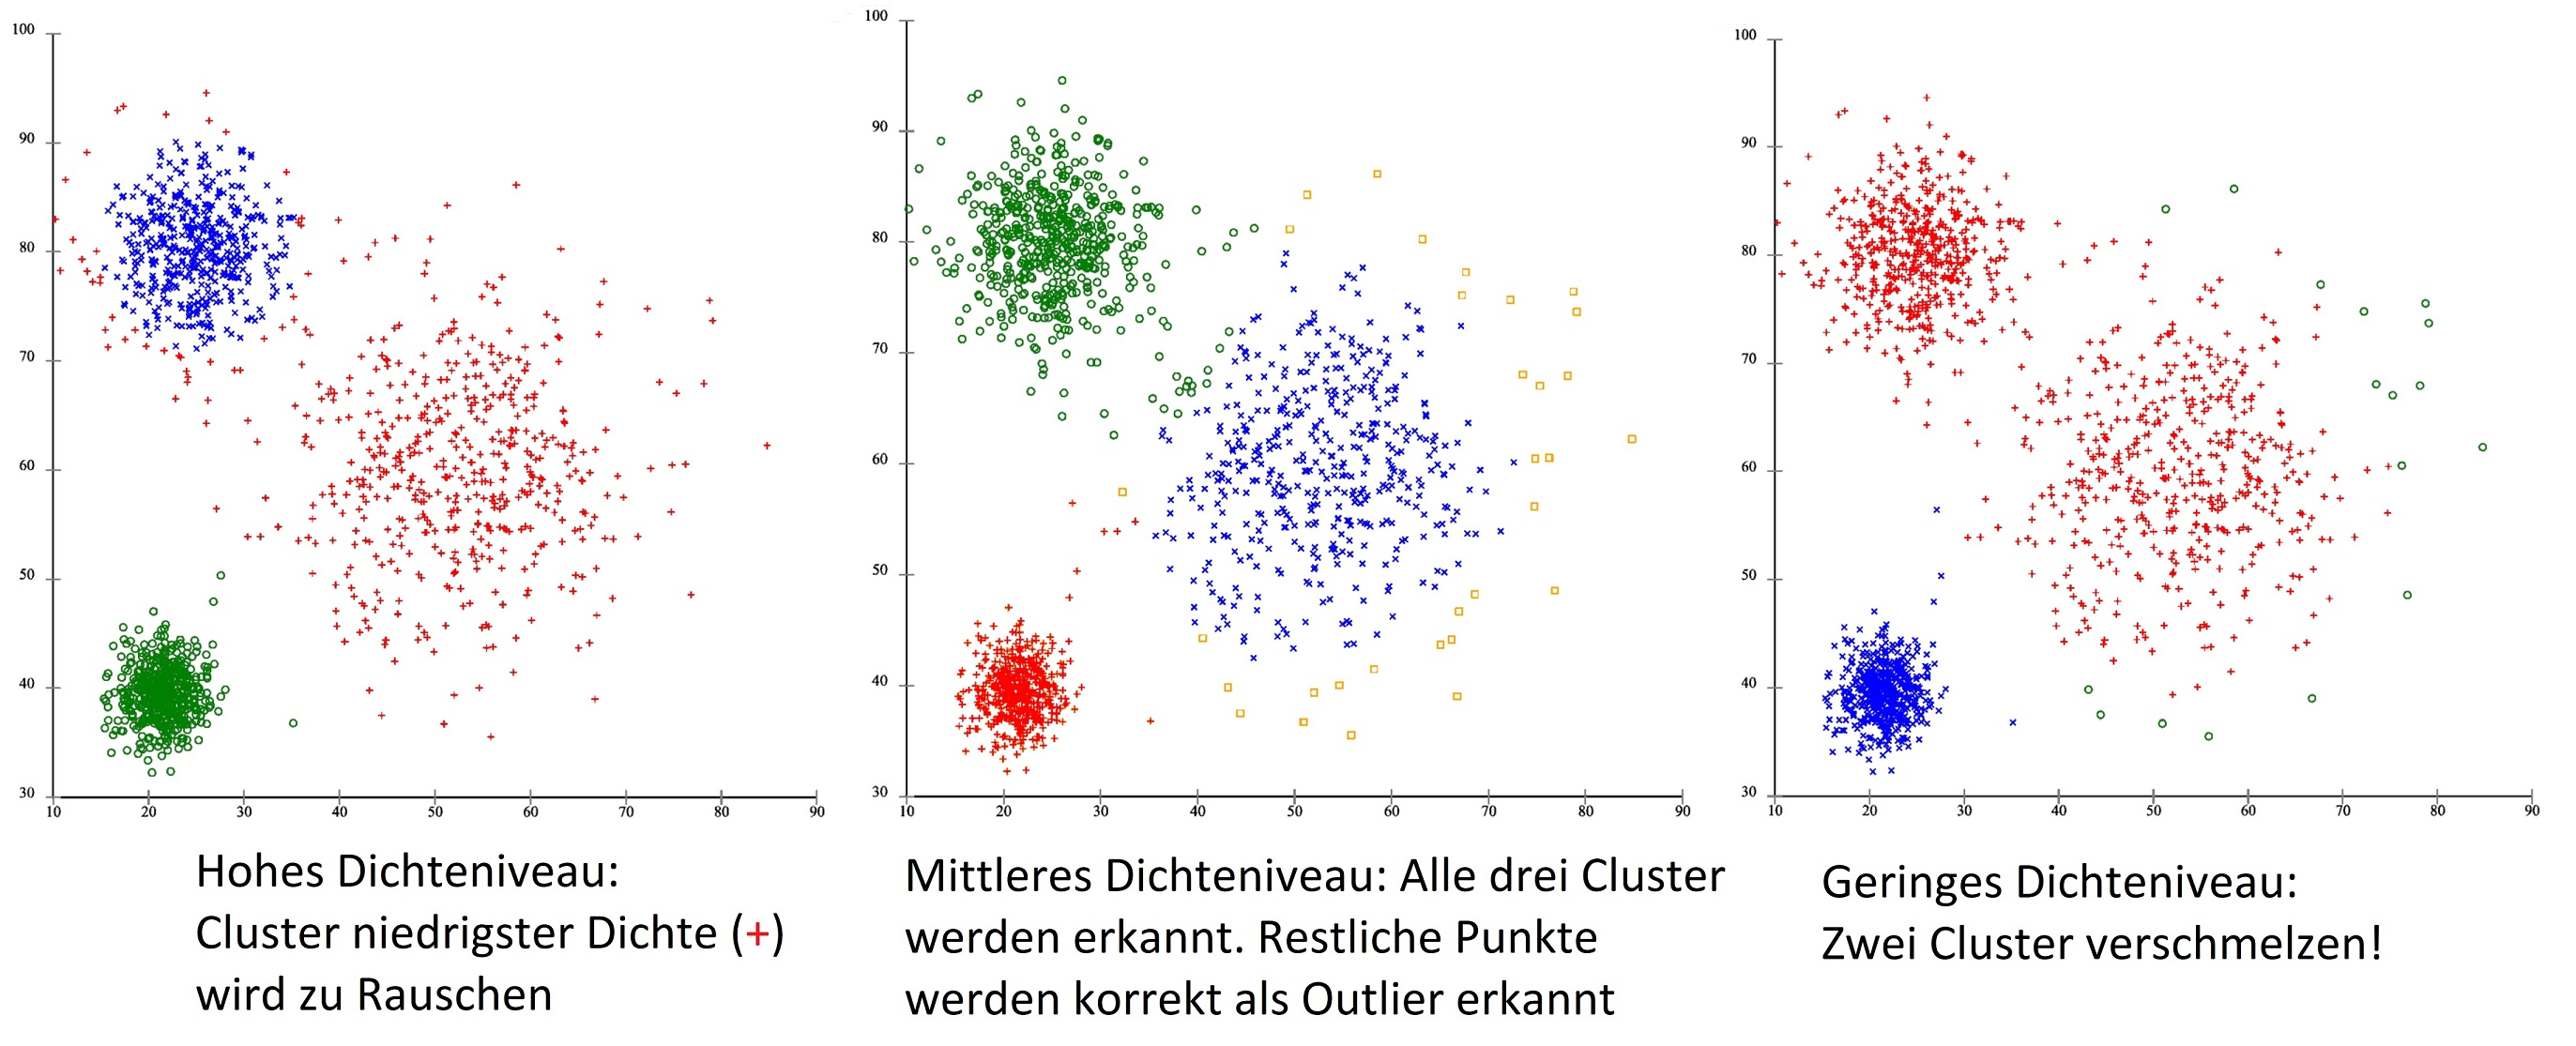
\includegraphics[scale=0.35]{dbscanprob.jpg}
\caption{Probleme von DBSCAN bei Erkennung von Clustern mit unterschiedlicher Dichte}
\label{dbscan_problems}
\end{figure}

\subsubsection{Erreichbarkeitseigenschaften \cite{dbscan}}
Die \textbf{$\epsilon$-Nachbarschaft} $N_\epsilon(p)$ ist die Menge aller Punkte, welche maximal $\epsilon$ Einheiten von $p$ entfernt sind.
 
Ein Punkt heißt \textbf{Kernobjekt}, wenn die Anzahl der Objekte in der $\epsilon$-Nachbarschaft mindestens $minPts$ beträgt, wobei $\epsilon$ und $minPts$ feste Werte sind, die dem Algorithmus initial übergeben werden. Sie spezifizieren zusammen die Grenzdichte eines Clusters.

\begin{minipage}{0.6\textwidth}\raggedright
Ein Objekt $o$ ist \textbf{direkt-dichte-erreichbar}, wenn es in der $\epsilon$-Nachbarschaft von $p$ liegt und $p$ ein Kernobjekt ist.
\end{minipage}
\hfill
\begin{minipage}{0.3\textwidth}
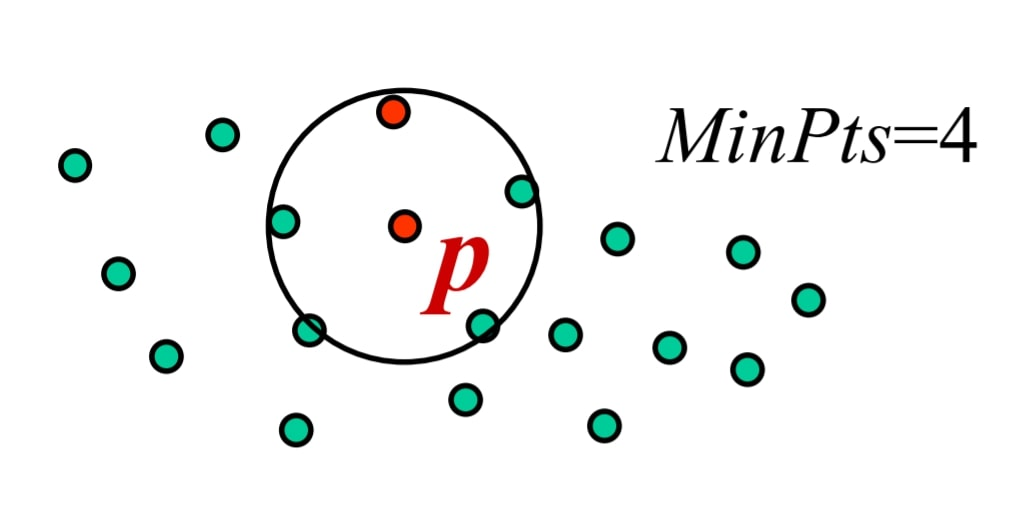
\includegraphics[width=\linewidth]{neps.jpg}
\end{minipage}


\begin{minipage}{0.6\textwidth}\raggedright
Ein Objekt $q$ ist \textbf{dichte-erreichbar}, wenn es eine Kette von direkt-dichte-erreichbaren Objekten von $p$ nach $q$ gibt.
\end{minipage}
\hfill
\begin{minipage}{0.3\textwidth}
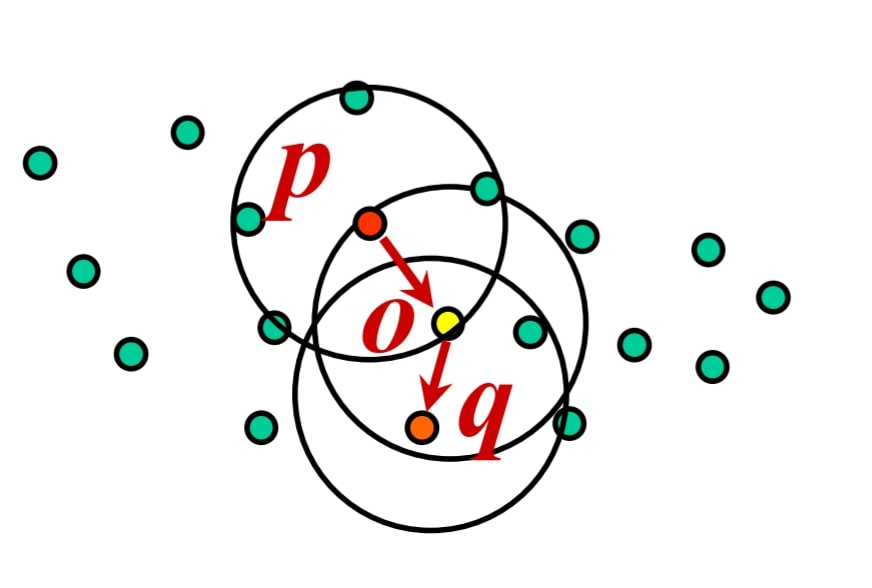
\includegraphics[width=\linewidth]{dichteerreichbar.jpg}
\end{minipage}

\begin{minipage}{0.6\textwidth}\raggedright
Zwei Objekte $p$ und $q$ sind \textbf{dichte-verbunden}, wenn es einen gemeinsamen Punkt $o$ gibt, von dem aus sowohl $p$ als auch $q$ dichte-erreichbar ist.
\end{minipage}
\hfill
\begin{minipage}{0.3\textwidth}
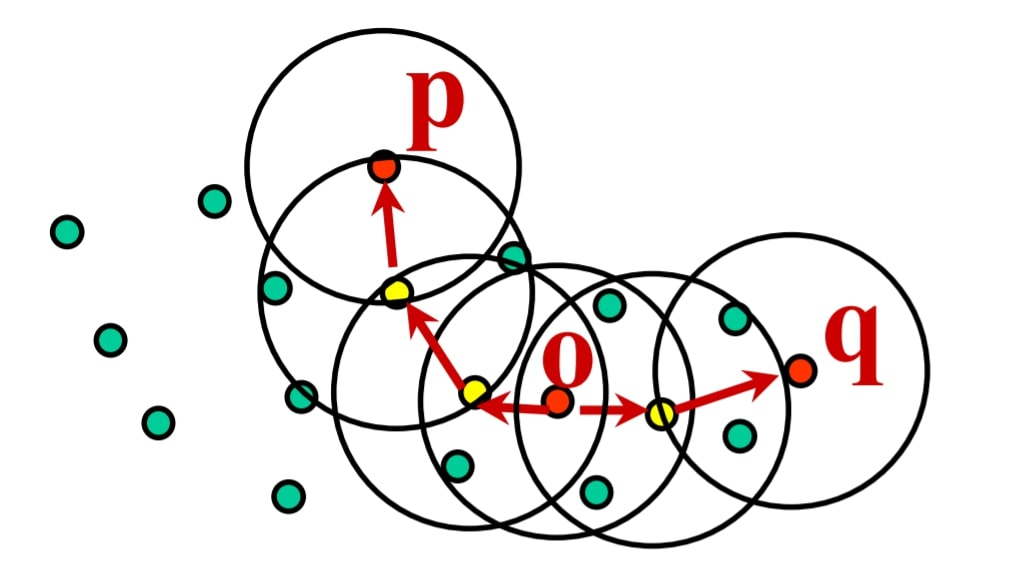
\includegraphics[width=\linewidth]{dichteverbunden.jpg}
\end{minipage}
\\~\\
Im Folgenden beschränke ich mich auf die hierarchische Variante des DBSCAN-Algorithmus, da sie in der Praxis besonders auf Geodatensätzen bessere Ergebnisse erzielt und das Problem aus Abbildung \ref{dbscan_problems} löst. Gegenüber der Grundvariante ist OPTICS allerdings rechenintensiver.

\subsubsection{Erweiterte Grundbegriffe}~
\begin{minipage}{0.50\textwidth}\raggedright
Die Kerndistanz $kd_{\epsilon, minPts}(o)$ ist genau dann definiert, wenn $o$ ein Kernobjekt ist, also in der $\epsilon$-Nachbarschaft mindestens $minPts$ Punkte liegen. Sie entspricht dann dem kleinsten Radius um $o$, der erforderlich ist, um $minPts$ Punkte einzuschließen.\\~\\

Die Erreichbarkeitsdistanz $rd_{\epsilon, minPts}(p ,o)$ ist genau dann definiert, wenn $o$ ein Kernobjekt ist. Sie entspricht dann der Kerndistanz von $o$, aber mindestens dem Abstand zwischen $p$ und $o$.
\end{minipage}
\hfill
\begin{minipage}{0.45\textwidth}
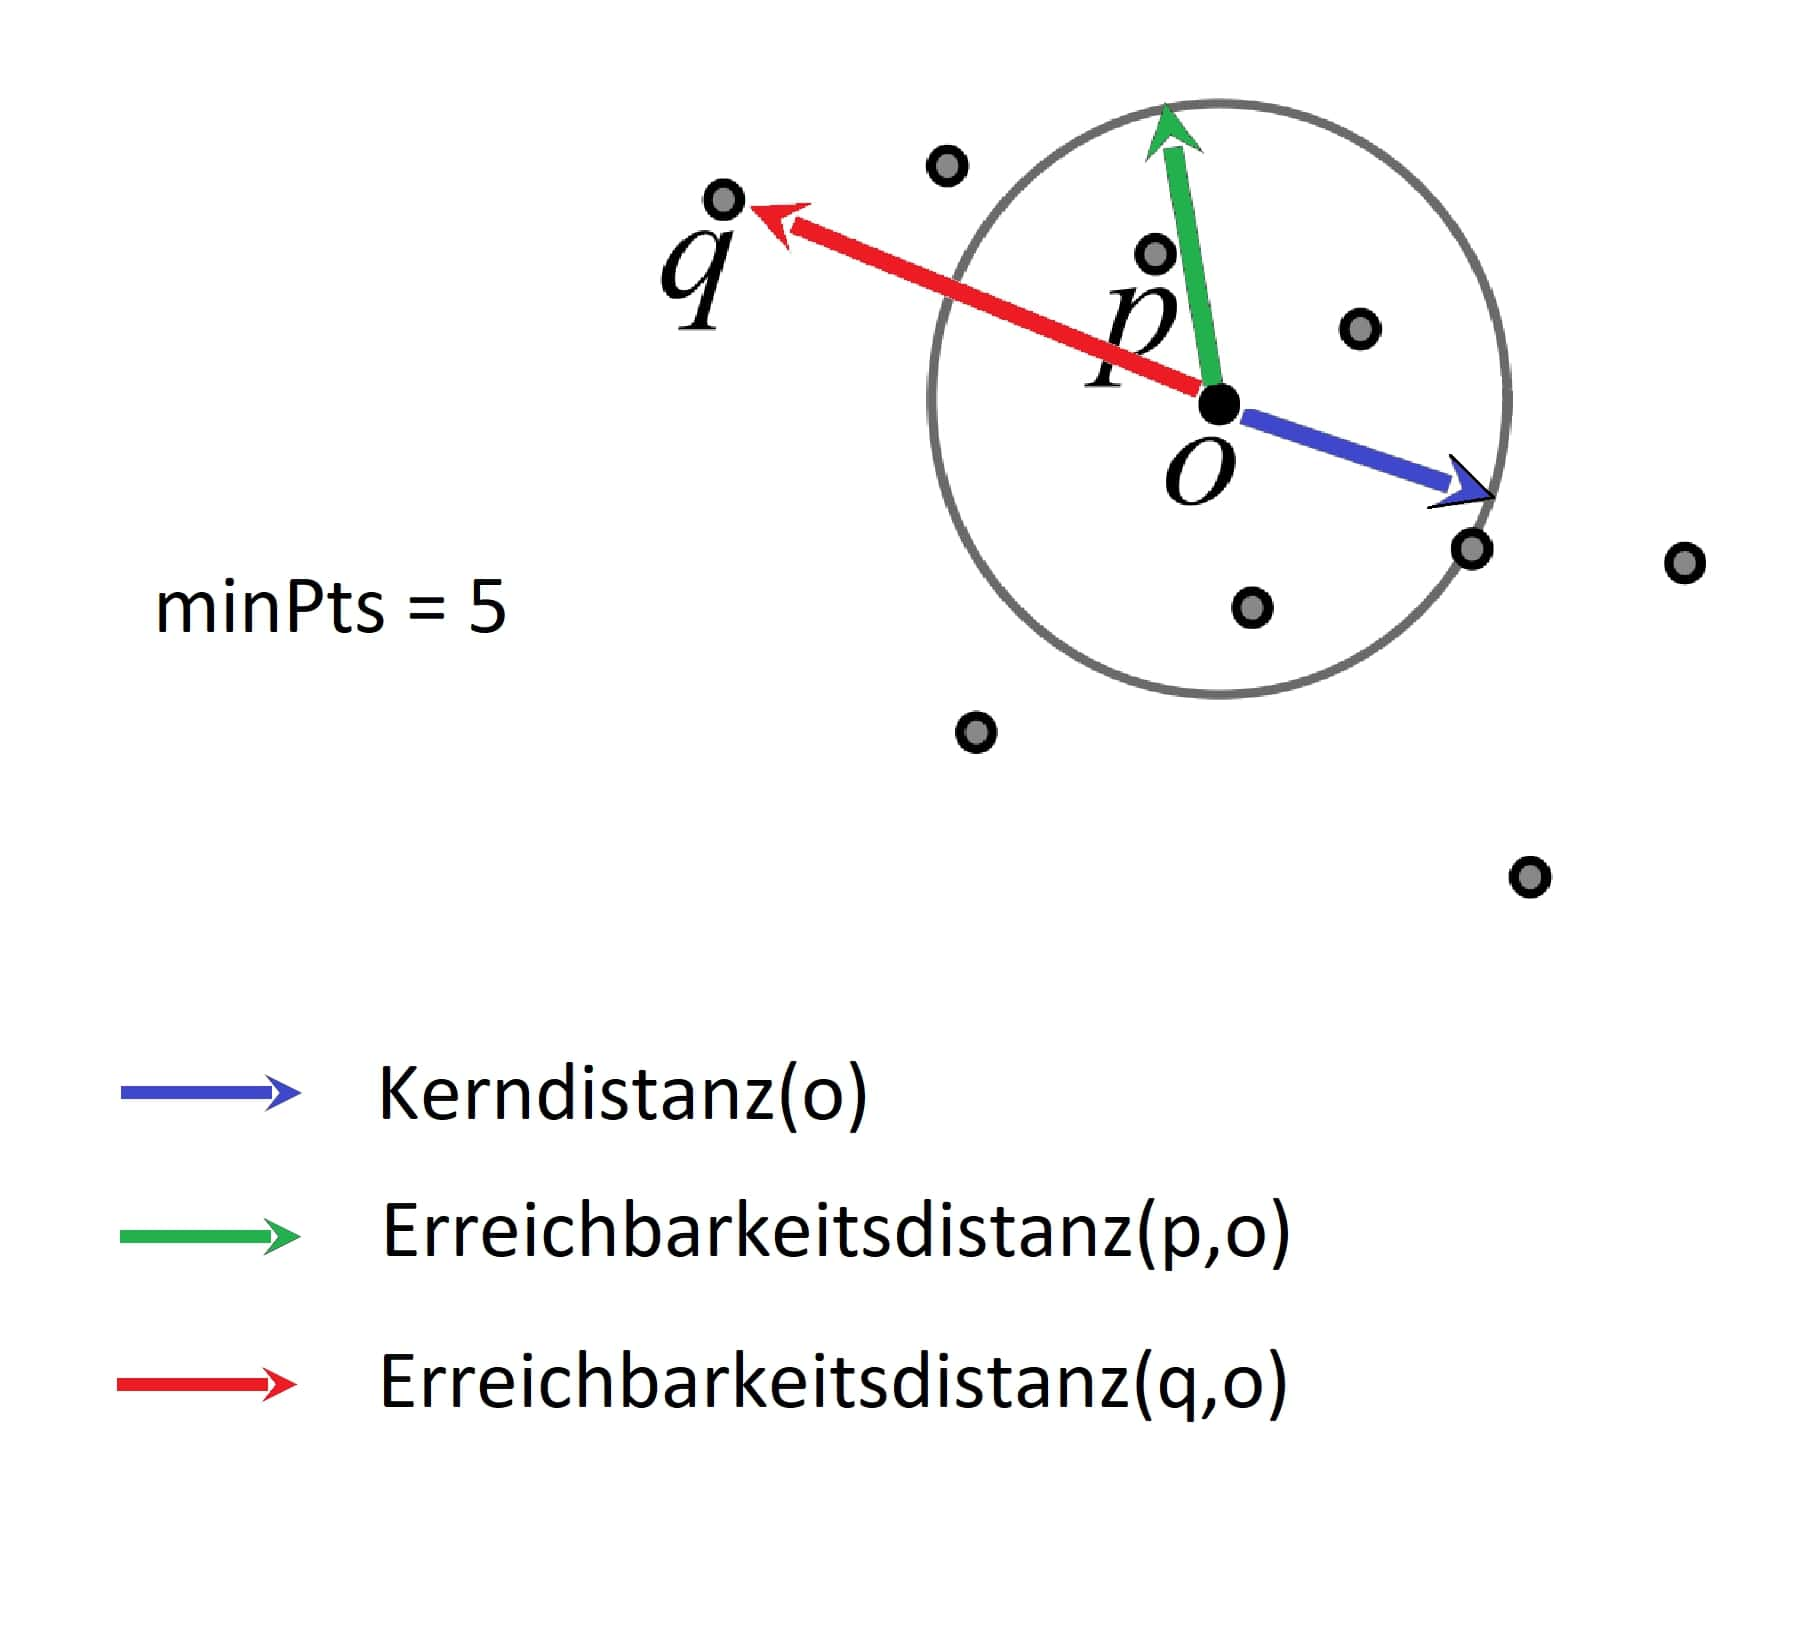
\includegraphics[width=\linewidth]{kdrd.jpg}
\end{minipage}
\\
Der OPTICS(Ordering Points To Identify the Clustering Structure)-Algorithmus \cite{optics} liefert bezüglich der Parameter $\epsilon$ und $minPts$ eine Ordnung von Clustern in Form eines Erreichbarkeitsdiagramms. Dazu werden die Punkte so sortiert, dass ein nachfolgender Punkt im Diagramm zur Menge der bereits besuchten Objekte die kleinste Erreichbarkeitsdistanz besitzt.

\begin{figure}[H]
\centering
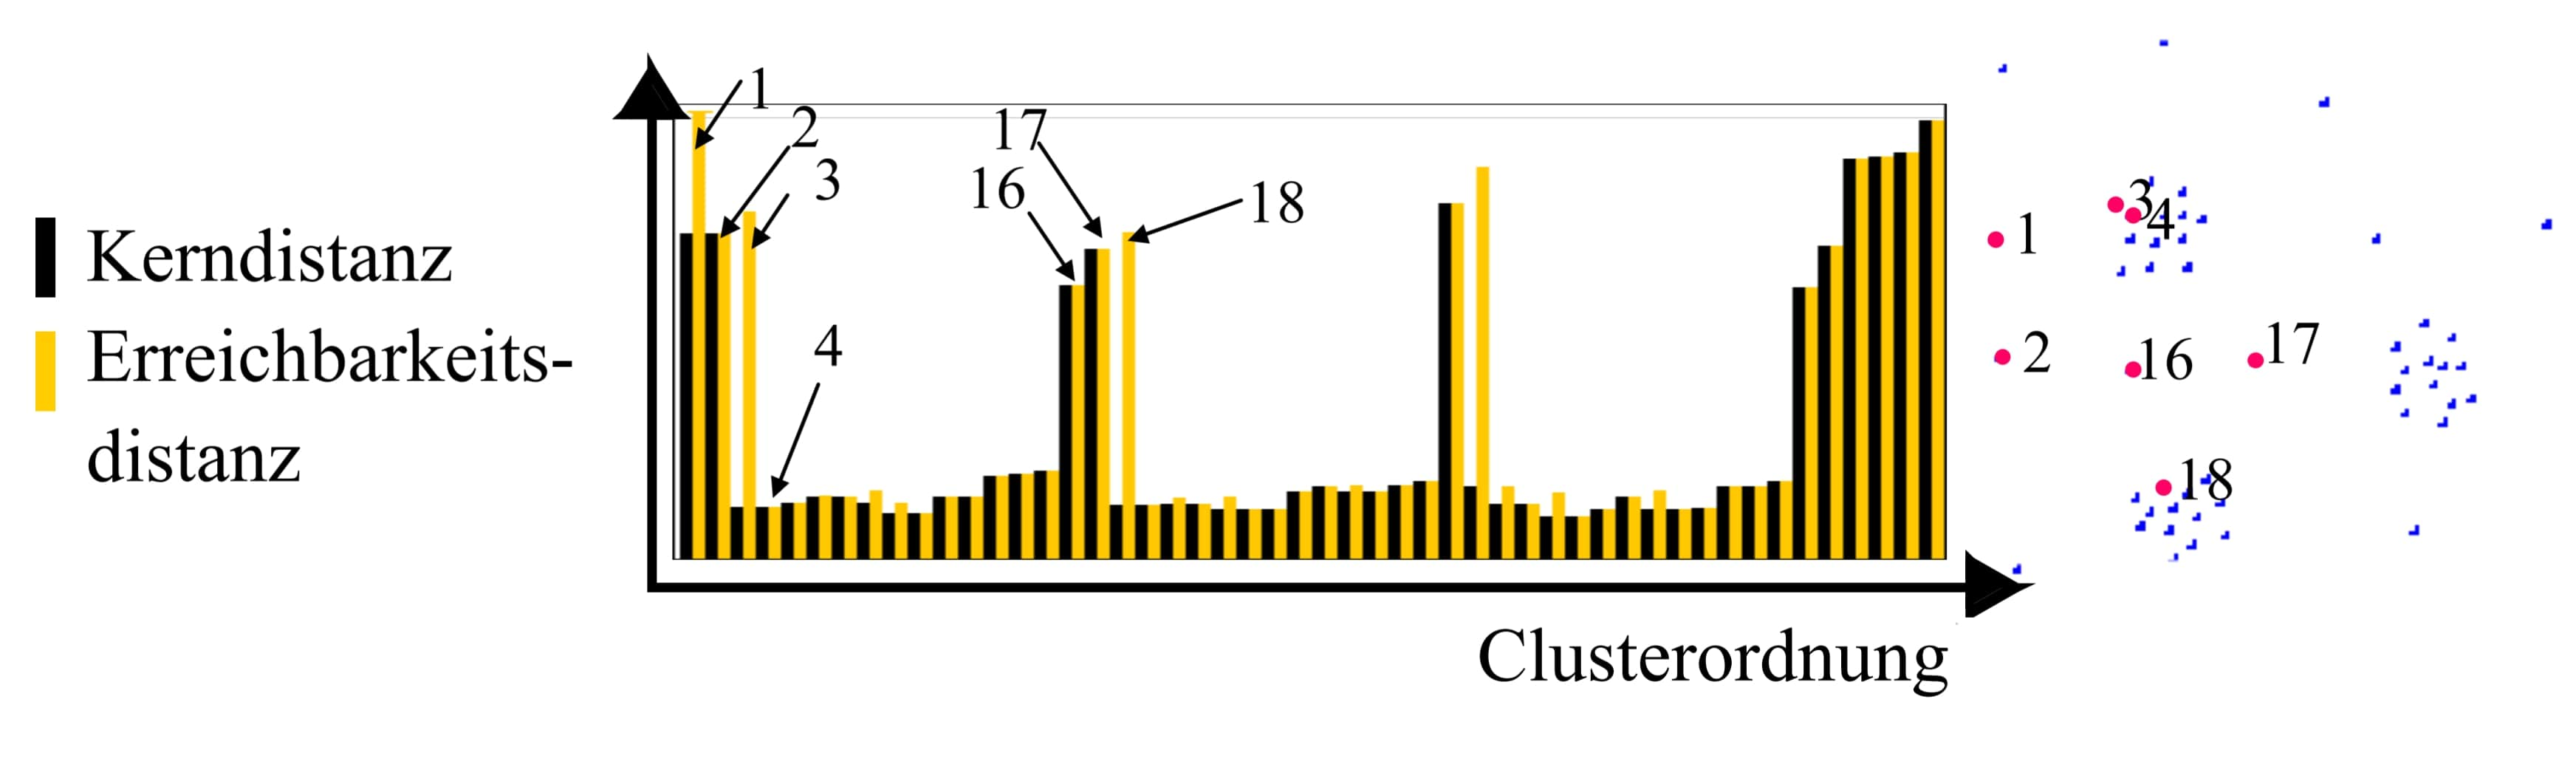
\includegraphics[scale=0.12]{reachdiag.jpg}
\caption{Erreichbarkeitsdiagramm (OrderedFile) nach Ausführung des OPTICS-Algorithmus\protect\footnotemark}
\end{figure}
\footnotetext{\url{http://www-old.dbs.ifi.lmu.de/Lehre/KDD/WS0708/skript/kdd-5-clustering_02.pdf}}

\subsubsection{OPTICS-Algorithmus}

Die äußere Schleife betrachtet jedes Objekt der Datenmenge $D$, welches noch nicht als bearbeitet markiert wurde und ruft \textit{ExpandClusterOrder} auf. Die Datei \textit{OrderedFiles} codiert das Erreichbarkeitsdiagramm.
\begin{minipage}{\linewidth} %Vermeidung von Seitenumbruch! 
\begin{lstlisting}[frame=single,mathescape=true]
OPTICS(Objektmenge D, Real $\epsilon$, Integer MinPts, OutputFile OrderedFile)
	OrderedFile.open();
	for i from 1 to D.size() do
		Objekt := D.get(i);
	if not Objekt.Bearbeitet then
		ExpandiereClusterOrder(D, Objekt, $\epsilon$, MinPts, OrderedFile);
OrderedFile.close();
\end{lstlisting}
\end{minipage}


\textit{ExpandClusterOrder} ist der eigentliche Algorithmus. Er bestimmt für den aktuell betrachteten Datenpunkt $O$ die $\epsilon$-Nachbarschaft und Kerndistanz, markiert ihn als bearbeitet und fügt ihn dem Erreichbarkeitsdiagramm hinzu. Die zuvor definierte Undefiniertheit der Erreichbarkeit des ersten Punktes im \textit{ExpandClusterOrder} wird als maximaler Wert (z.B. $\infty$) interpretiert. Wenn $O$ ein Kernobjekt ist, wird $update(Nachbarn, O)$ aufgerufen. Das bedeutet, dass in der Pufferdatei \textit{OrderSeeds}, in welcher die Nachbarn des Zentrumsobjekt für ihre Abarbeitung vorsortiert werden, operiert wird. Alle $\epsilon$-Nachbarn von $O$ werden dieser Liste hinzugefügt, sofern sie noch nicht enthalten sind und aufsteigend nach ihrer Erreichbarkeitsdistanz zu $O$ sortiert. Ist ein Nachbar schon enthalten, so wird sein Erreichbarkeitswert aktualisiert, wenn die neue Erreichbarkeitsdistanz kleiner ist als die Vorherige.
Anschließend wird eine innere Schleife ausgeführt. In dieser werden alle Objekte der Pufferdatei ähnlich wie das Zentrumsobjekt abgearbeitet, bis kein Element mehr übrig ist. Wird \textit{ExpandClusterOrder} verlassen, kann kein weiteres Objekt dem aktuellen Cluster zugeordnet werden und der Algorithmus wird mit einem zufälligen anderen Objekt fortgesetzt, das noch nicht bearbeitet wurde. Anschließend wird auch dessen Cluster expandiert.

\begin{minipage}{\linewidth}
\begin{lstlisting}[frame=single,mathescape=true]
ExpandClusterOrder(Objektmenge D, Objekt O, 
		Real $\epsilon$, Integer MinPts, OutputFile OrderedFile):
	Nachbarn:= D.bestimmeNachbarschaft(O, $\epsilon$);
	O.Erreichbarkeitsdistanz:= UNDEFINIERT;
	O.setzeKerndistanz(Nachbarn, $\epsilon$, MinPts);
	O.Bearbeitet:= TRUE;
	OrderedFile.write(o);
	if O.Kerndistanz $\neq$ UNDEFINIERT then // Objekt O ist Kernobjekt
		OrderSeeds.update(Nachbarn, O);
		while OrderSeeds $\neq$ $\emptyset$ do
			aktObjekt := OrderSeeds.next();
			Nachbarn := D.bestimmeNachbarschaft(aktObjekt, eps);
			aktObjekt.setzeKerndistanz(Nachbarn, eps, MinPts);
			aktObjekt.Bearbeitet := TRUE;
			OrderedFile.write(aktObjekt);
			if aktObjekt.Kerndistanz $\neq$ UNDEFINIERT then
				OrderSeeds.update(Nachbarn, aktObjekt)
\end{lstlisting}
\end{minipage}

\begin{minipage}{\linewidth}
\begin{lstlisting}[frame=single,mathescape=true]
OrderSeeds :: update(Nachbarn, ZentrumsObjekt):
	c_dist := ZentrumsObjekt.Kerndistanz;
		for each Objekt from Nachbarn do
			if not Objekt.Bearbeitet then
				new r_dist := max(c_dist, ZentrumsObjekt.dist(Objekt));
				if Objekt.Erreichbarkeitsdistanz == UNDEFINIERT then
					Objekt.Erreichbarkeitsdistanz := new r_dist;
					insert(Objekt, new r_dist);
				else // Objekt ist schon in OrderSeeds enthalten
					if new_r_dist < Objekt.Erreichbarkeitsdistanz then
						Objekt.Erreichbarkeitsdistanz := new r_dist;
						decrease(Objekt, new r_dist);
\end{lstlisting}
\end{minipage}
\\~\\
Folgendes Beispiel soll den Ablauf des Algorithmus veranschaulichen:

Sei $\epsilon = 44$ und $minPts = 3$. Die betrachtete Datenbank hat 16 zweidimensionale Punkte (von A - H). Zu Beginn sind alle Objekte unbearbeitet und das Erreichbarkeitsdiagramm ist leer. 
\begin{figure}[H]
\centering
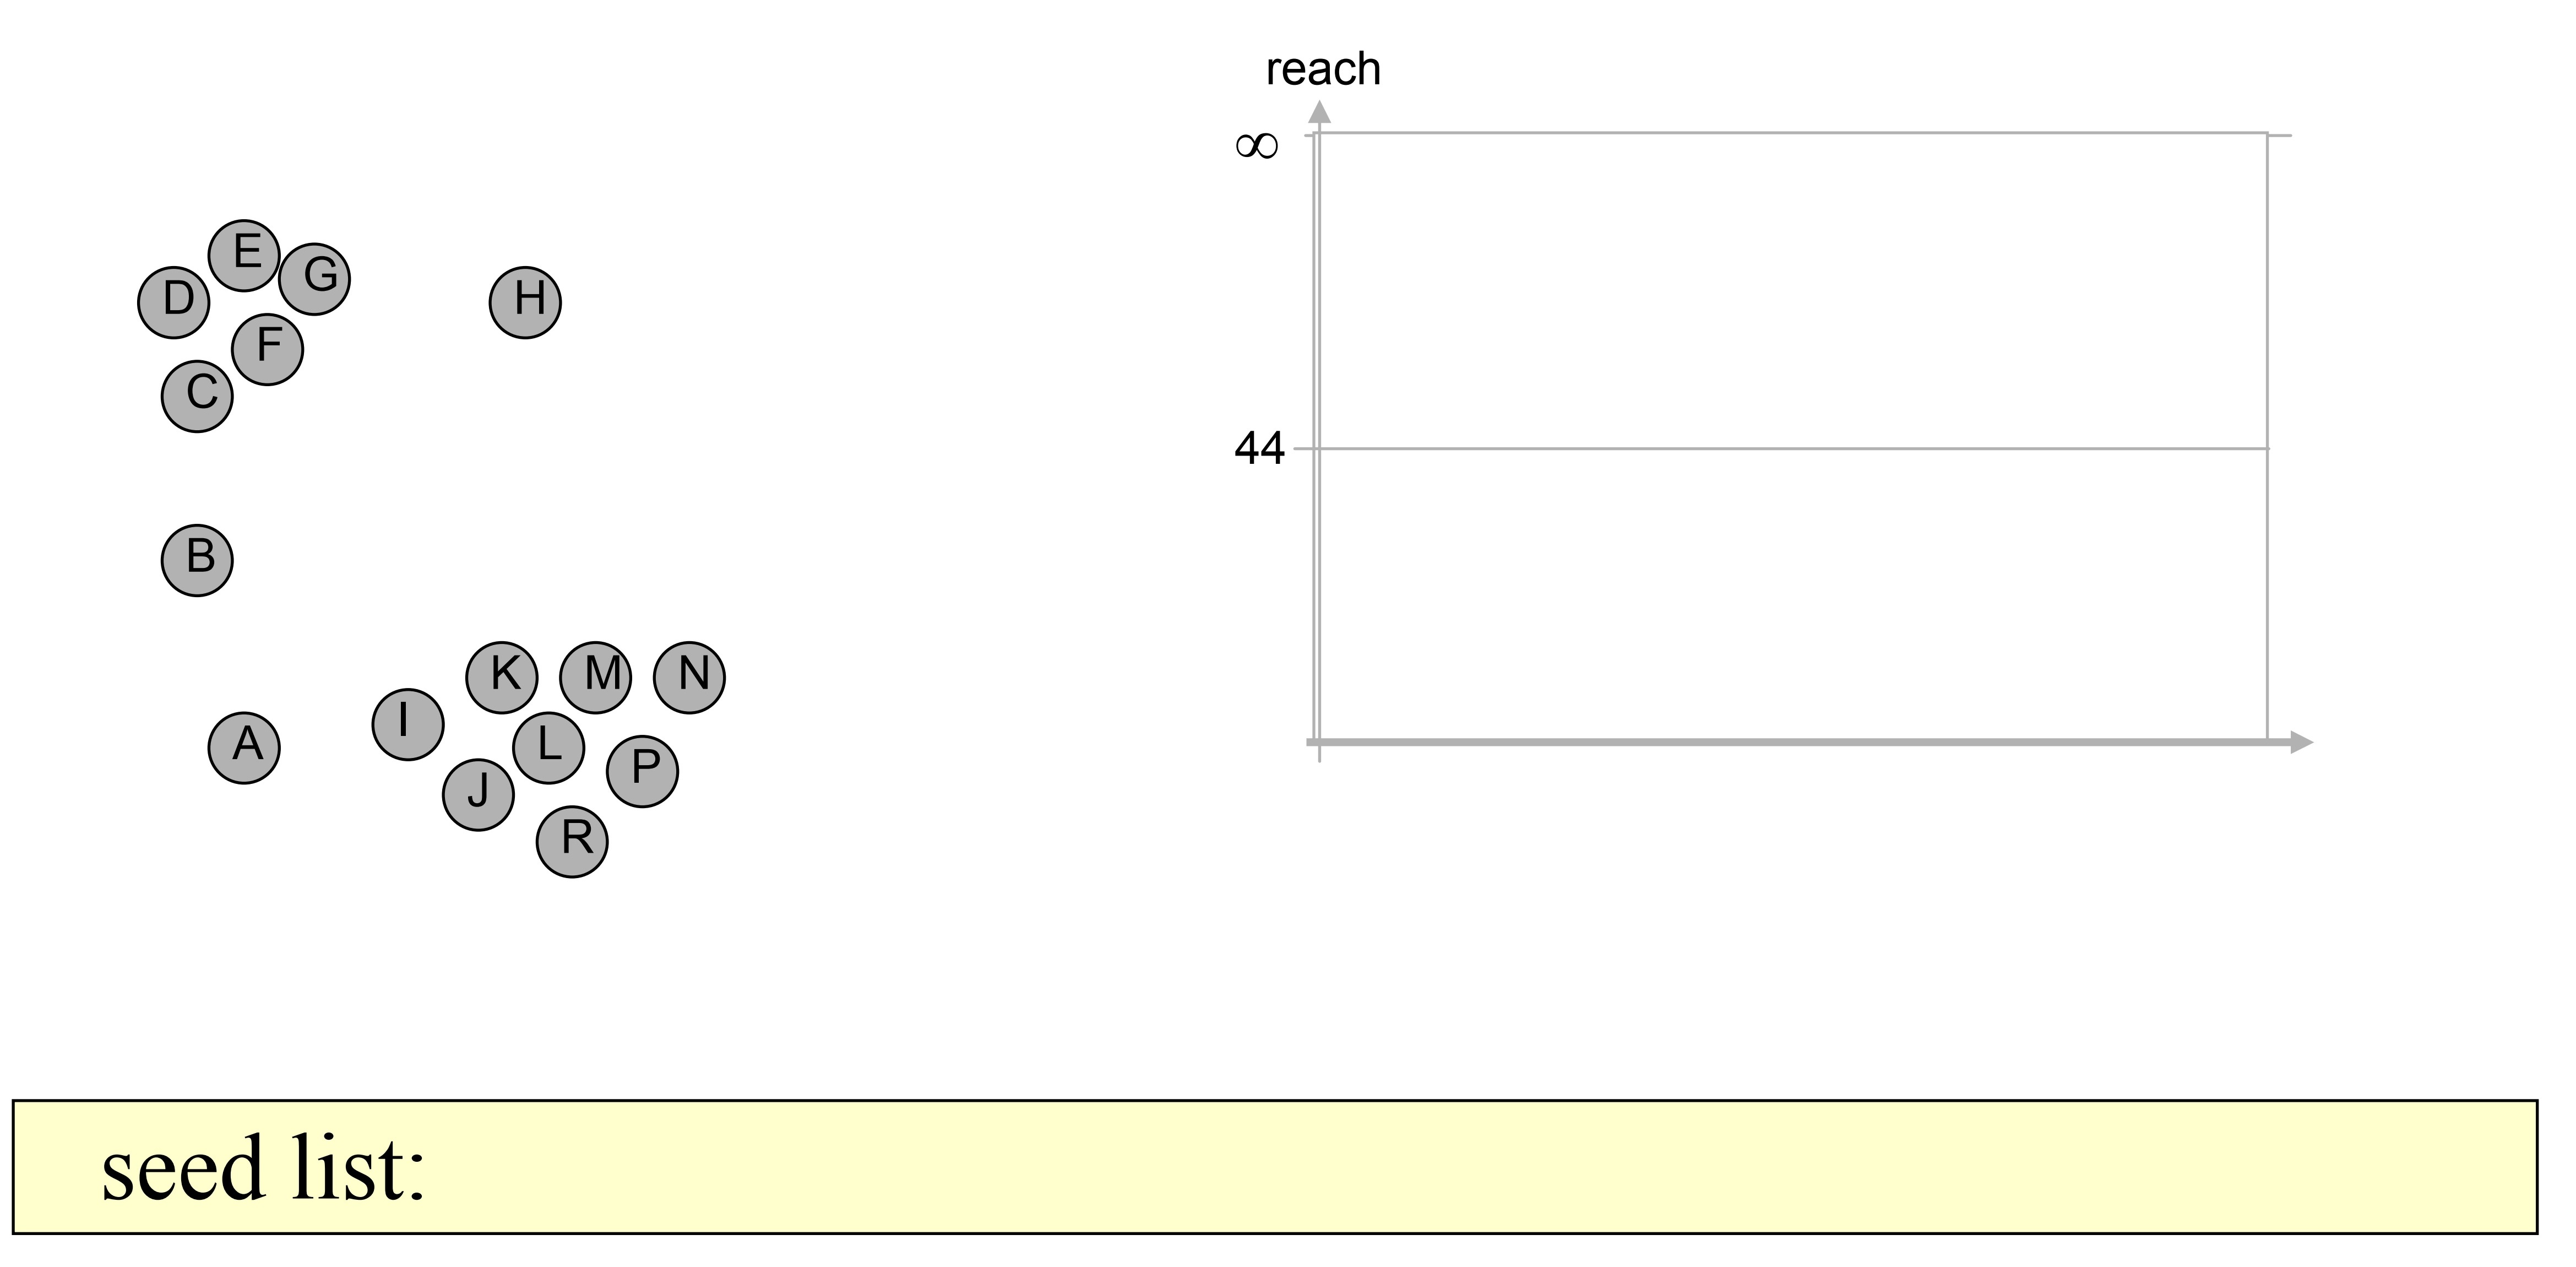
\includegraphics[scale=0.15]{opt1.jpg}
\end{figure}
Sei $A$ der erste Punkt. Die Erreichbarkeitsdistanz ist somit undefiniert. Die Kerndistanz ist definiert, da innerhalb des Radius $44$ die $minPts = 3$ Punkte $A$, $B$ und $I$ liegen. Die Kerndistanz von $A$ ist die Distanz zum am weitesten entfernten Punkt in der $\epsilon$-Nachbarschaft, also $40$. Jetzt wird der Punkt $A$ dem Erreichbarkeitsdiagramm mit dem Wert $\infty$ hinzugefügt und als bearbeitet markiert. Anschließend werden alle $\epsilon$-Nachbarn von $A$ inklusive ihrer Erreichbarkeitsdistanzen der Seeds-Liste hinzugefügt (Zeile 9, \textit{ExpandClusterOrder} erreicht).
\begin{figure}[H]
\centering
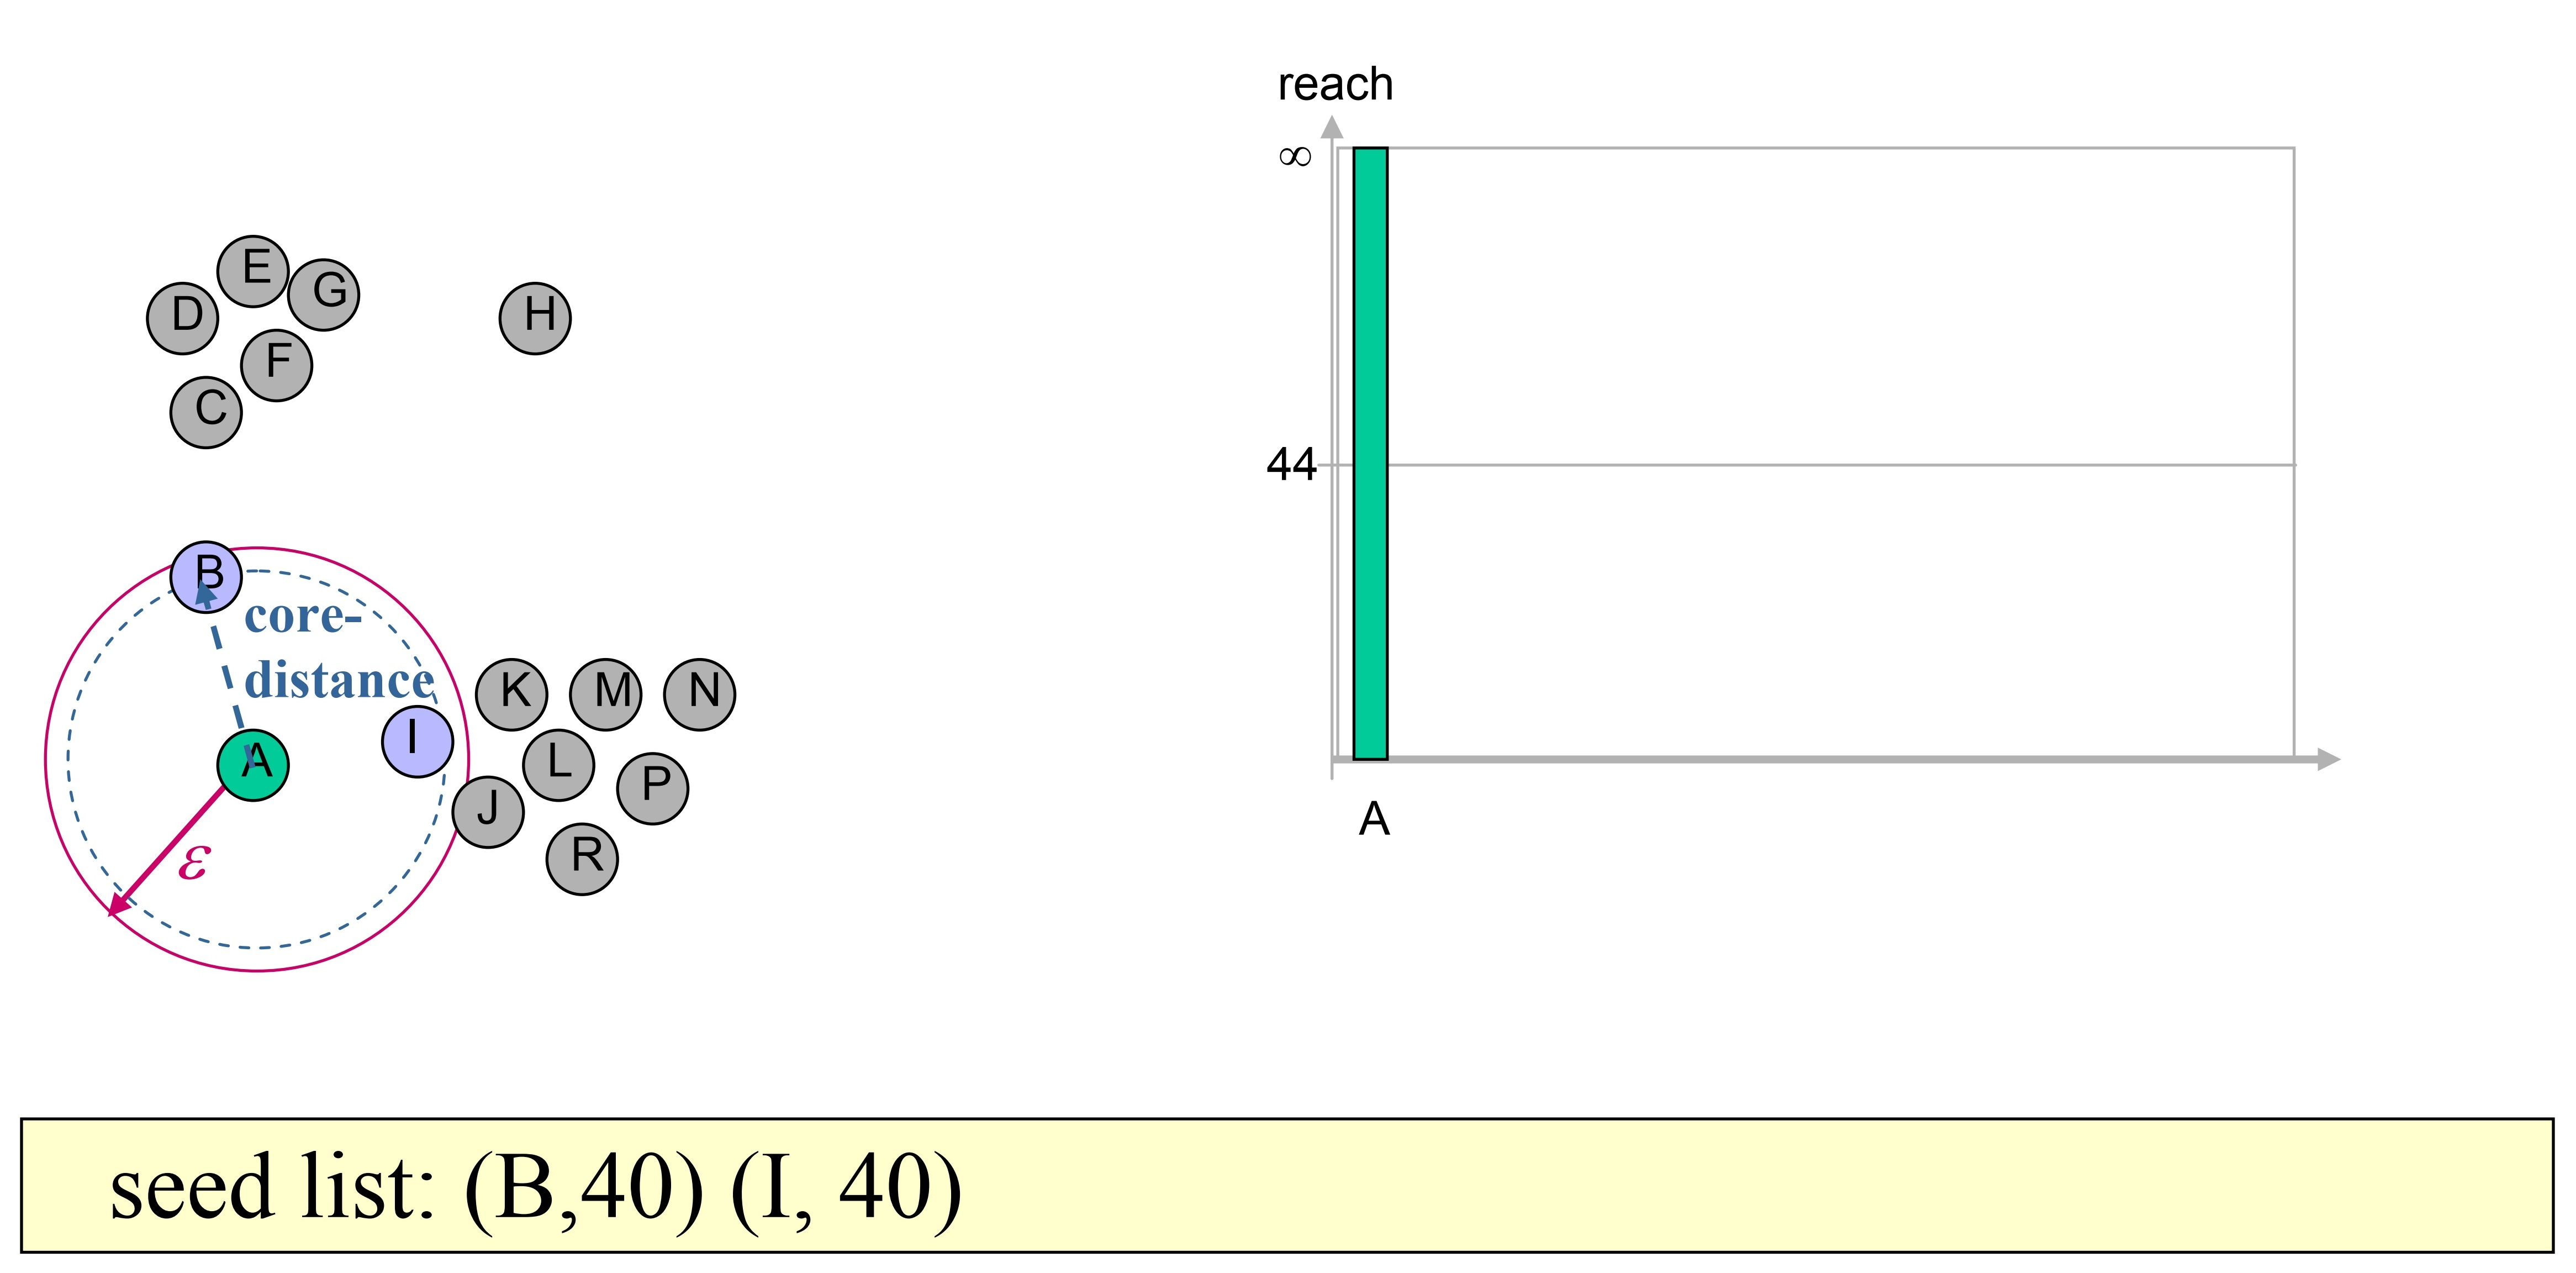
\includegraphics[scale=0.15]{opt2.jpg}
\end{figure}
Im nächsten Schritt (Zeile 10) wird über alle Objekte der Seeds-Liste iteriert. Das vorderste Objekt ist der Punkt $B$, in dessen $\epsilon$-Nachbarschaft wieder drei Punkte liegen ($A$, $B$ und $C$). Also ist auch $B$ ein Kernobjekt und die Kerndistanz lautet $40$. Nun wird Punkt $B$ als bearbeitet markiert und seine Erreichbarkeit dem Diagramm hinzugefügt. Da das Objekt $C$ noch nicht in der Seeds-Liste ist, wird es hinzugefügt.
\begin{figure}[H]
\centering
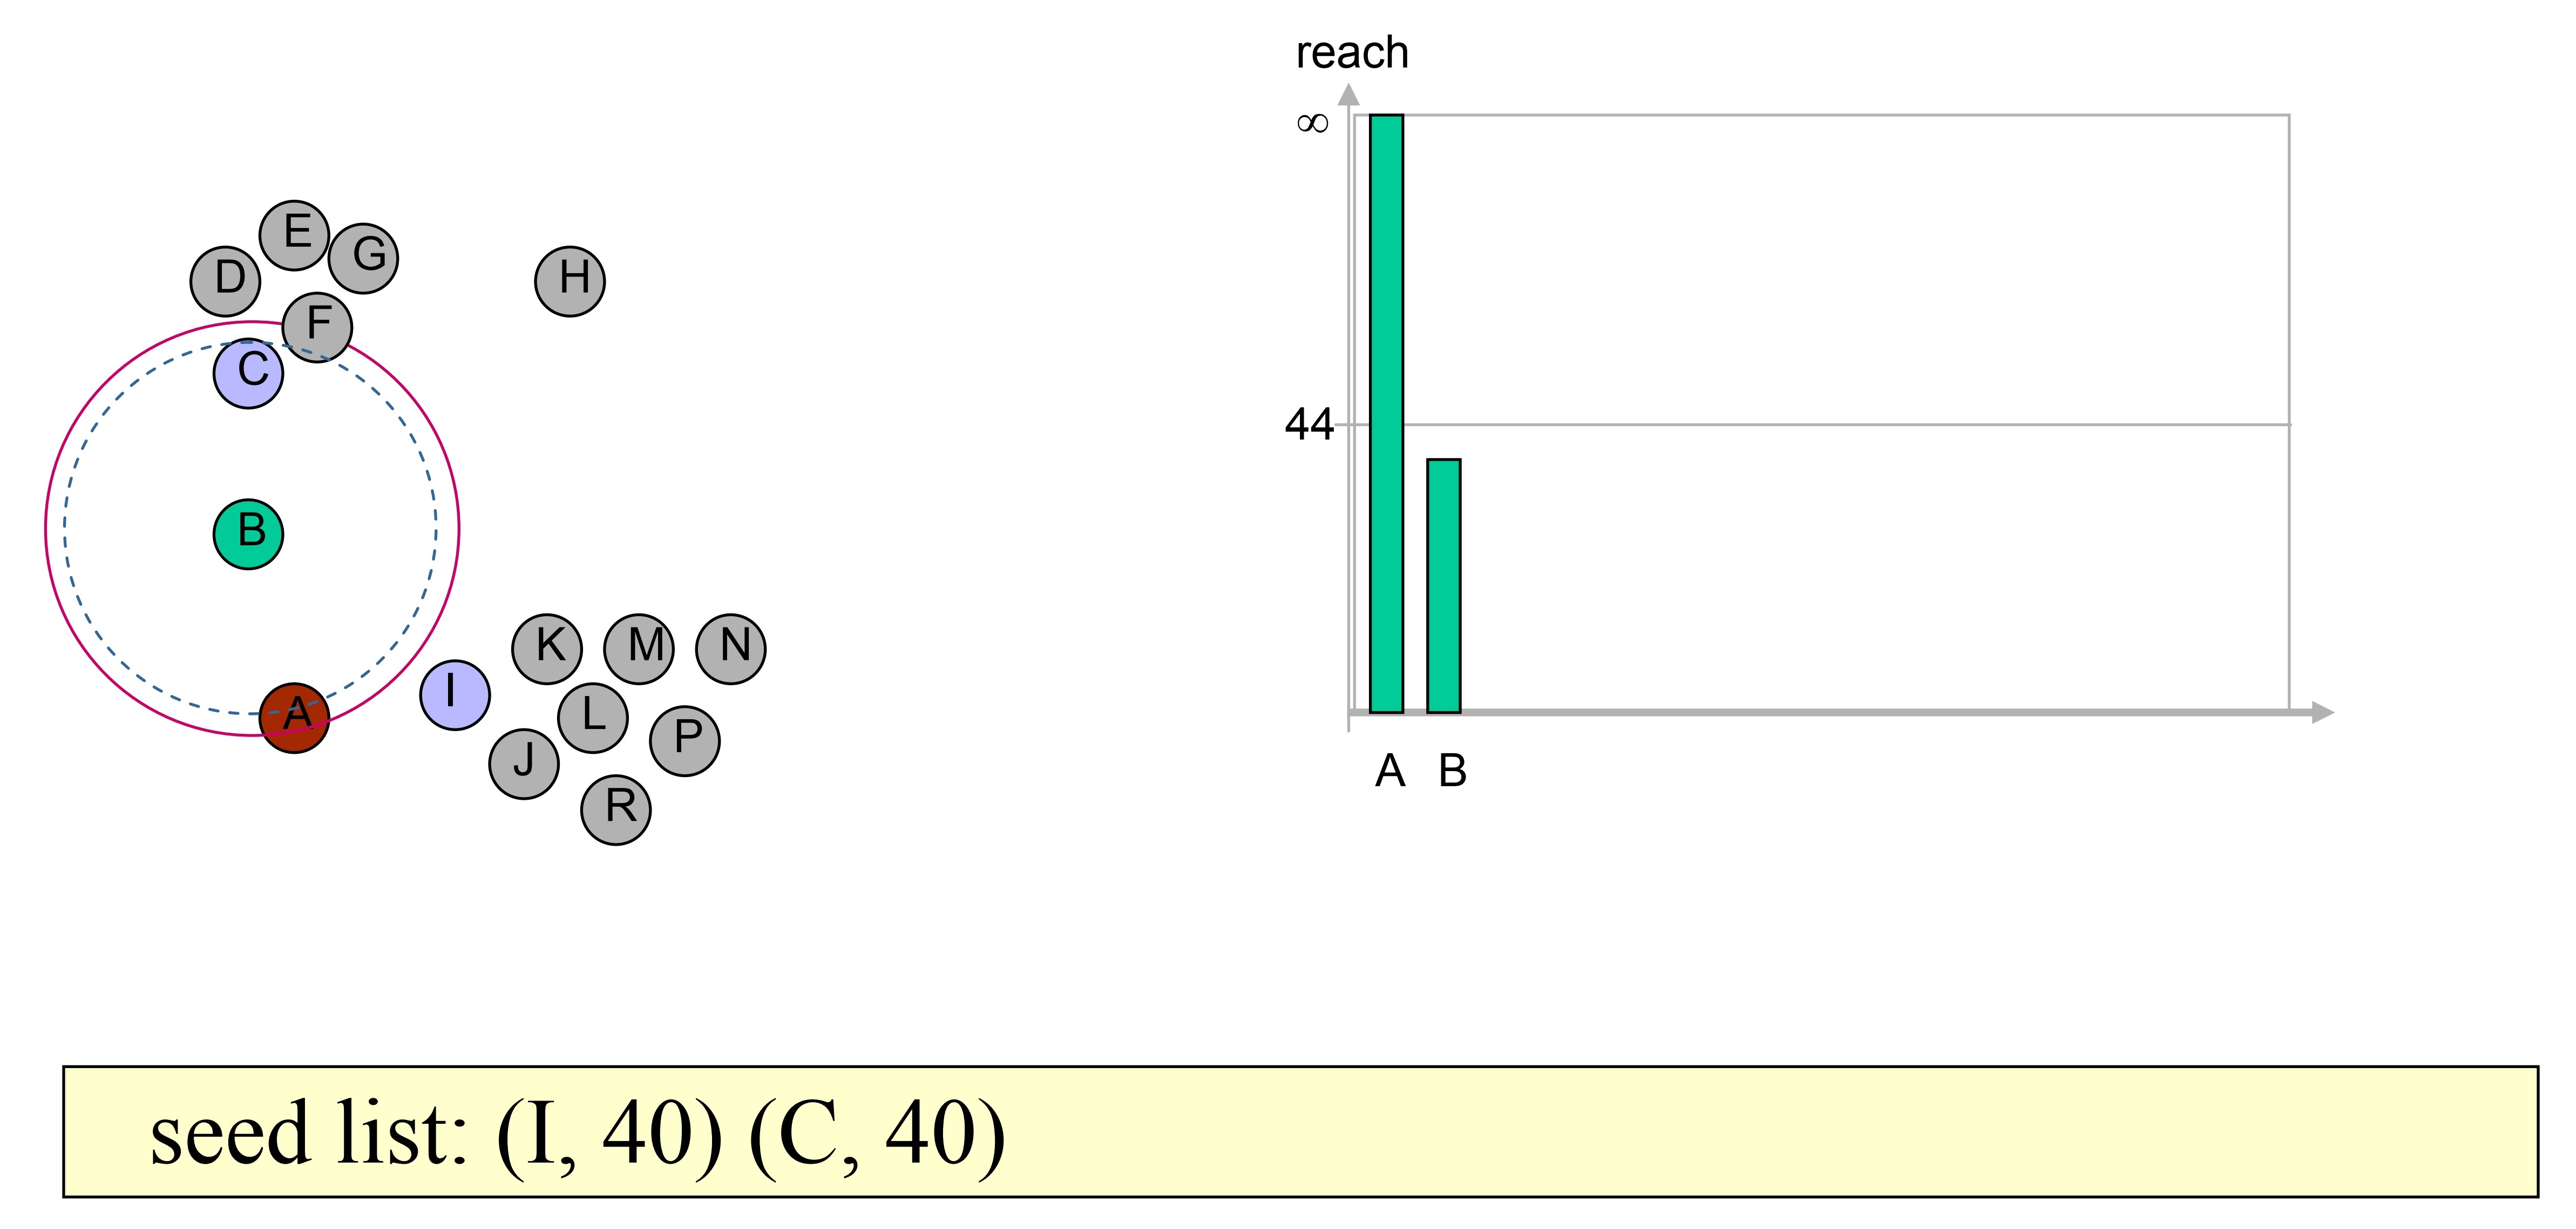
\includegraphics[scale=0.15]{opt3.jpg}
\end{figure}
Das nächste Objekt der Seeds-Liste ist der Punkt $I$. Auch dieser ist wieder ein Kernobjekt und hat 7 Punkte in seiner $\epsilon$-Nachbarschaft. Davon werden $K$, $J$, $M$, $L$ und $R$ der Seeds-Liste hinzugefügt.
\begin{figure}[H]
\centering
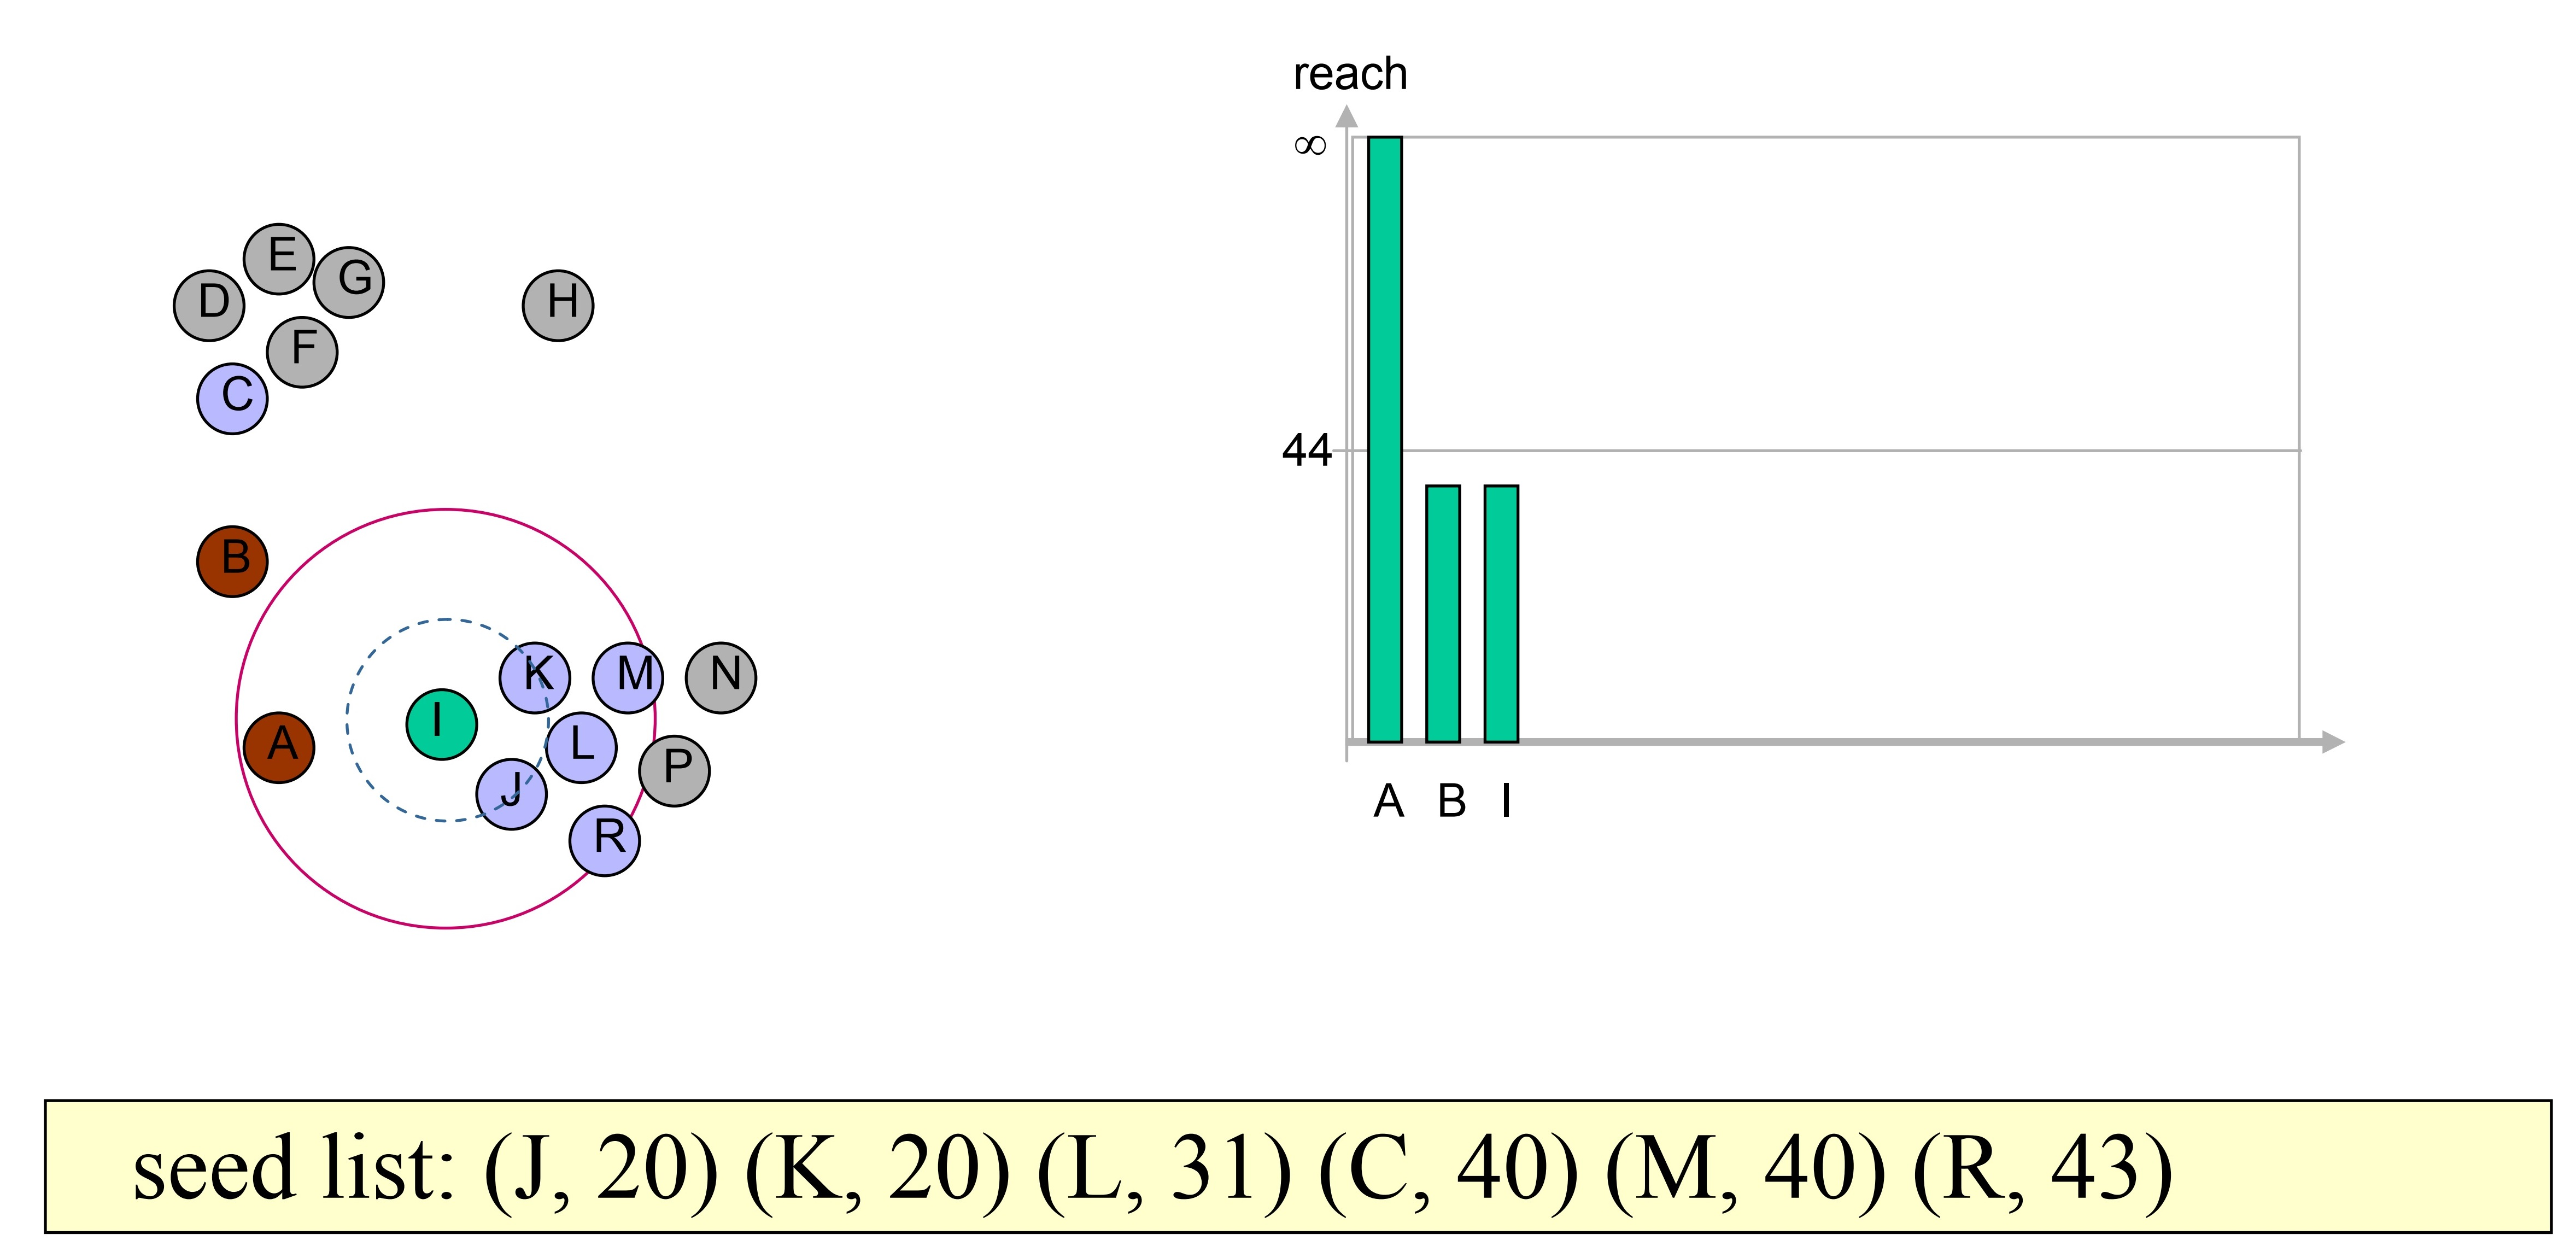
\includegraphics[scale=0.15]{opt4.jpg}
\end{figure}

Der Algorithmus setzt sich fort, bis ein Objekt bearbeitet wurde, für das kein weiterer unbearbeiteter $\epsilon$-Nachbar hinzugefügt werden konnte. In diesem Fall kommt es zu einem Peak im Erreichbarkeitsdiagramm, welcher den Beginn eines Subclusters kennzeichnet. Wird die Seeds-Liste leer und muss die äußere Schleife einen neuen zufälligen Startpunkt auswählen, beginnt ein neuer Cluster. 
In diesem Fall jedoch wird die innere Schleife fortgesetzt, da das Objekt $C$ noch in der Seeds-Liste steht.
\begin{figure}[H]
\centering
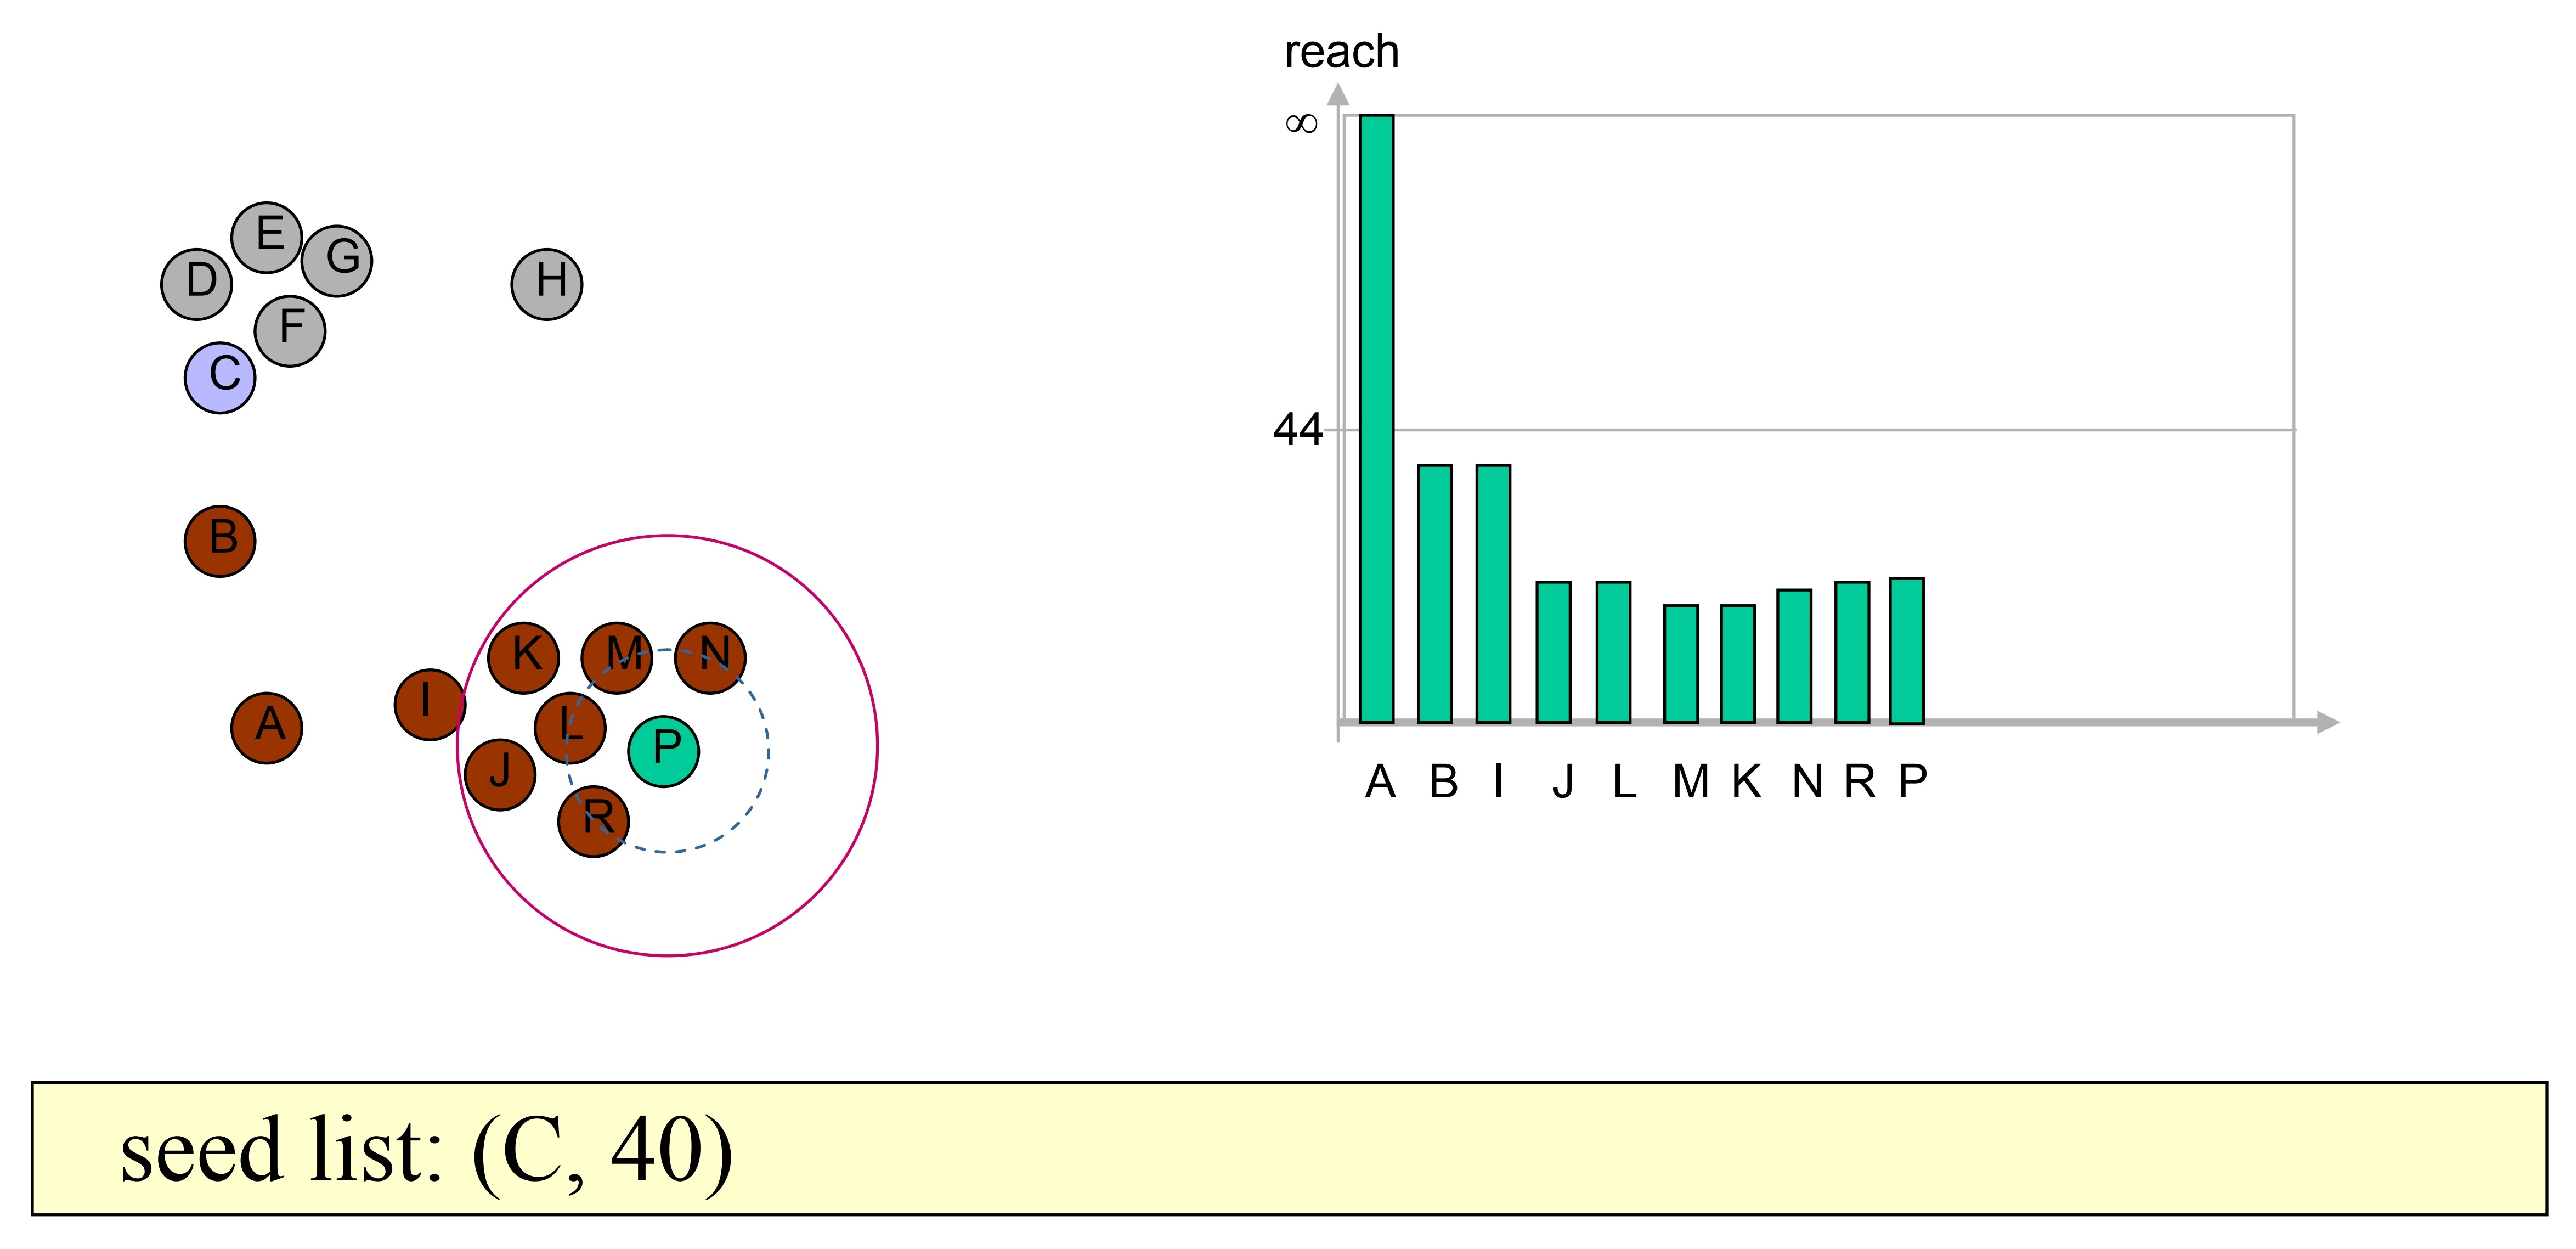
\includegraphics[scale=0.15]{opt5.jpg}
\end{figure}
Da $C$ ein Kernpunkt ist, werden dessen $\epsilon$-Nachbarn $D$, $F$, $E$ und $G$ der Seeds-Liste hinzugefügt. 
\begin{figure}[H]
\centering
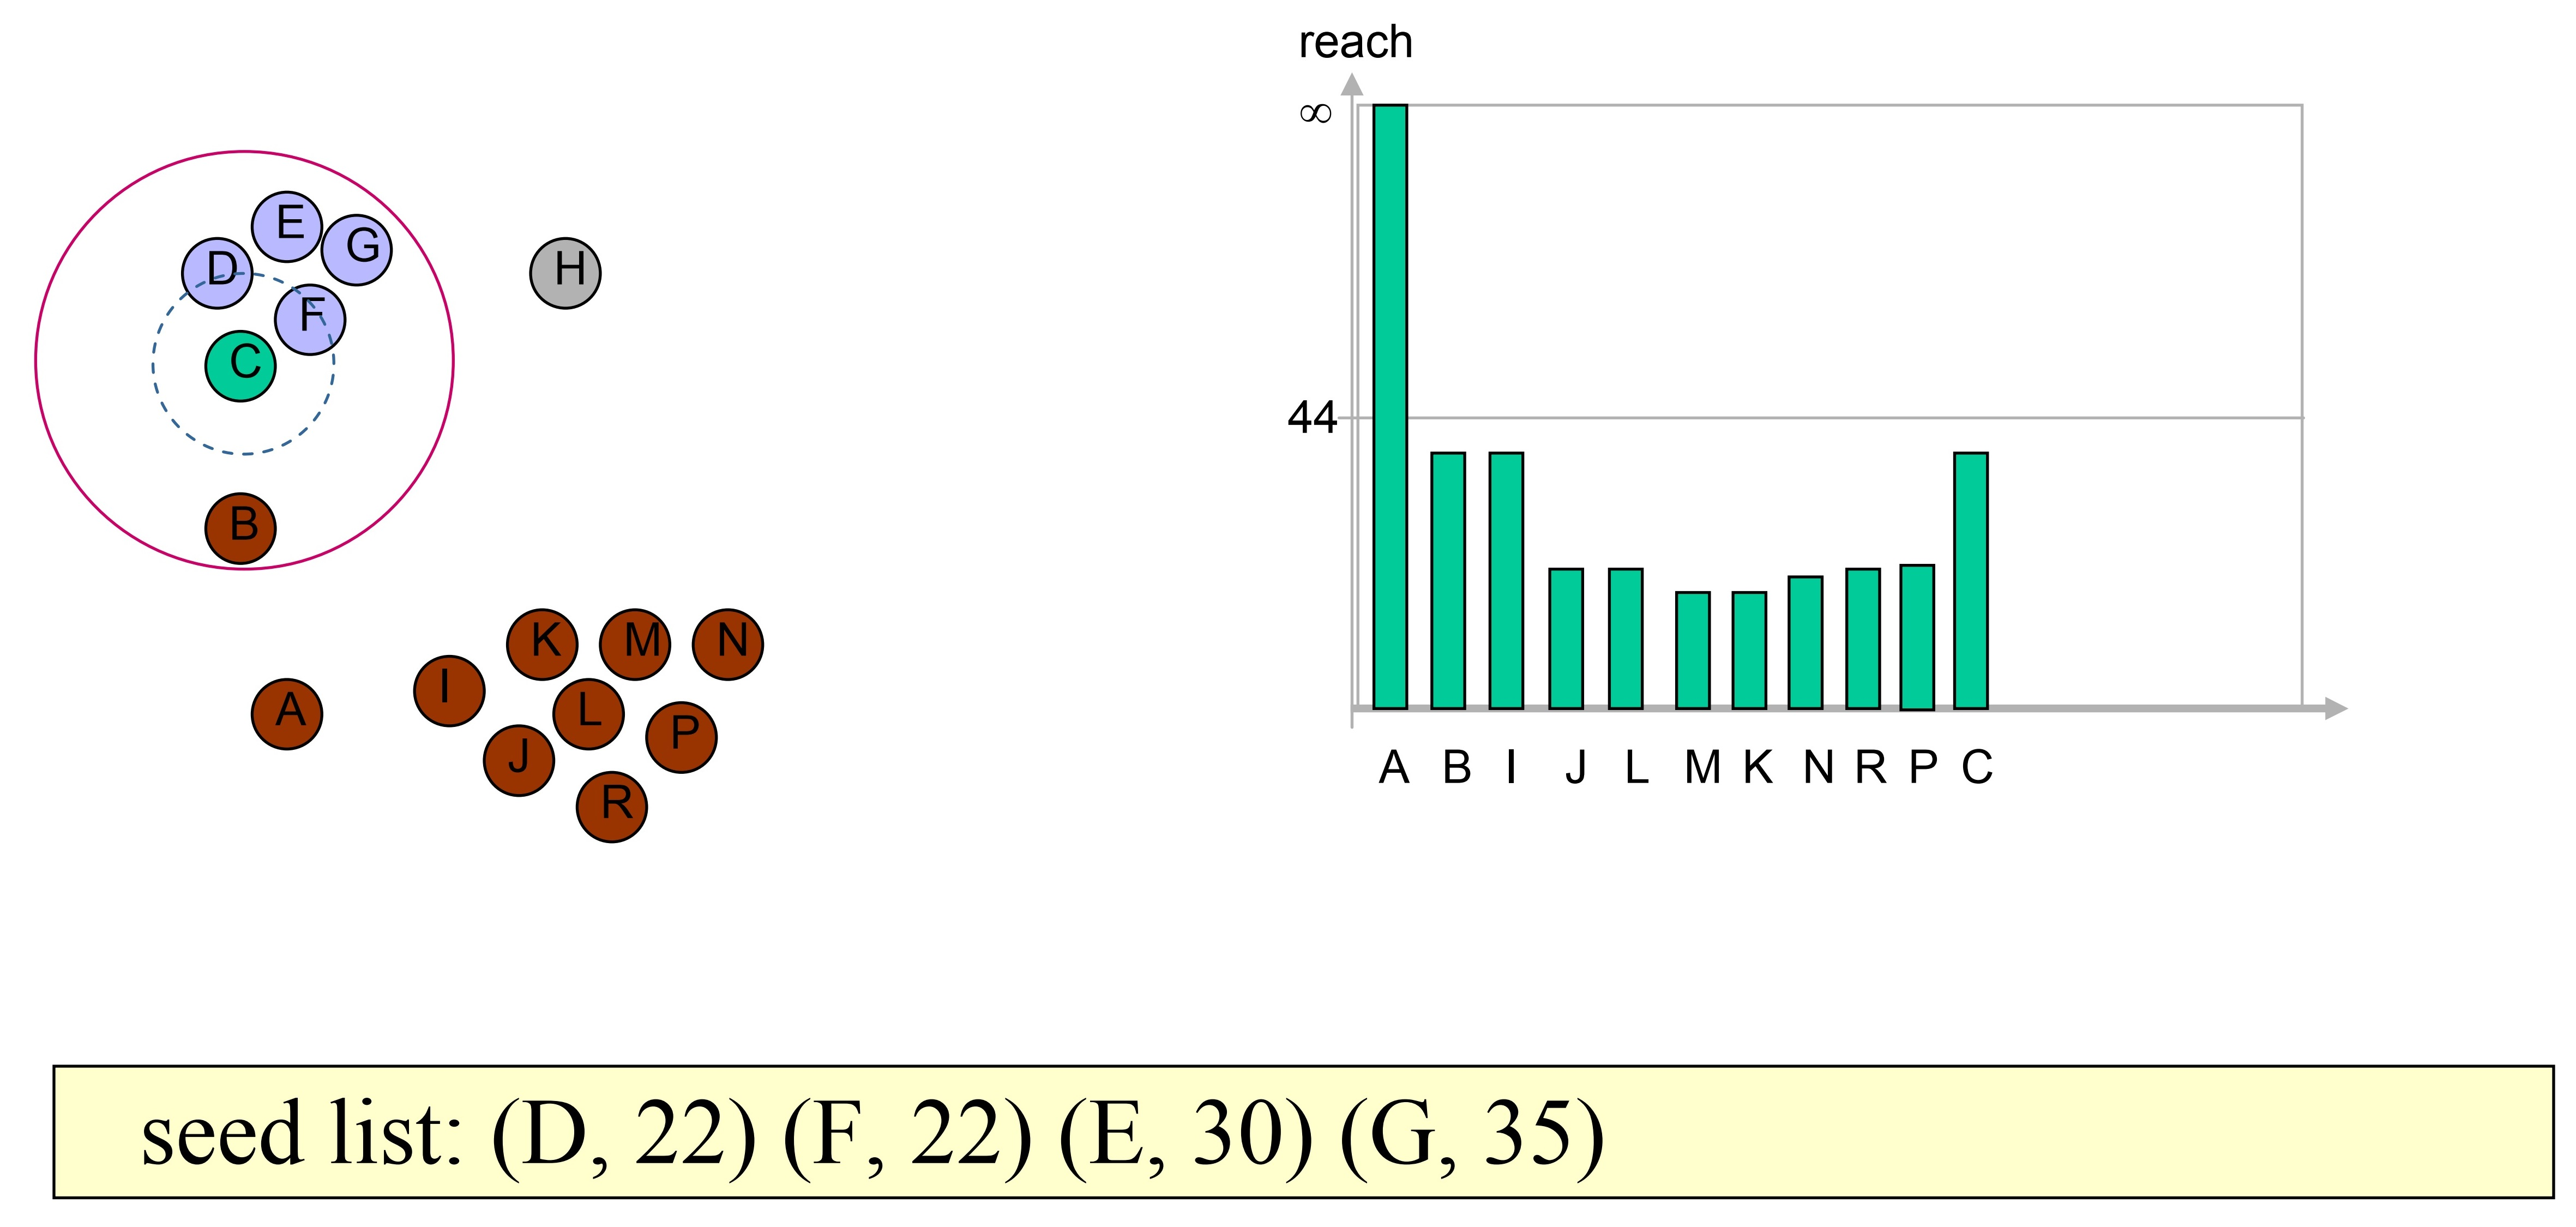
\includegraphics[scale=0.15]{opt6.jpg}
\end{figure}
Der Algorithmus setzt sich fort, bis es kein unbearbeitetes Objekt mehr gibt.
\begin{figure}[H]
\centering
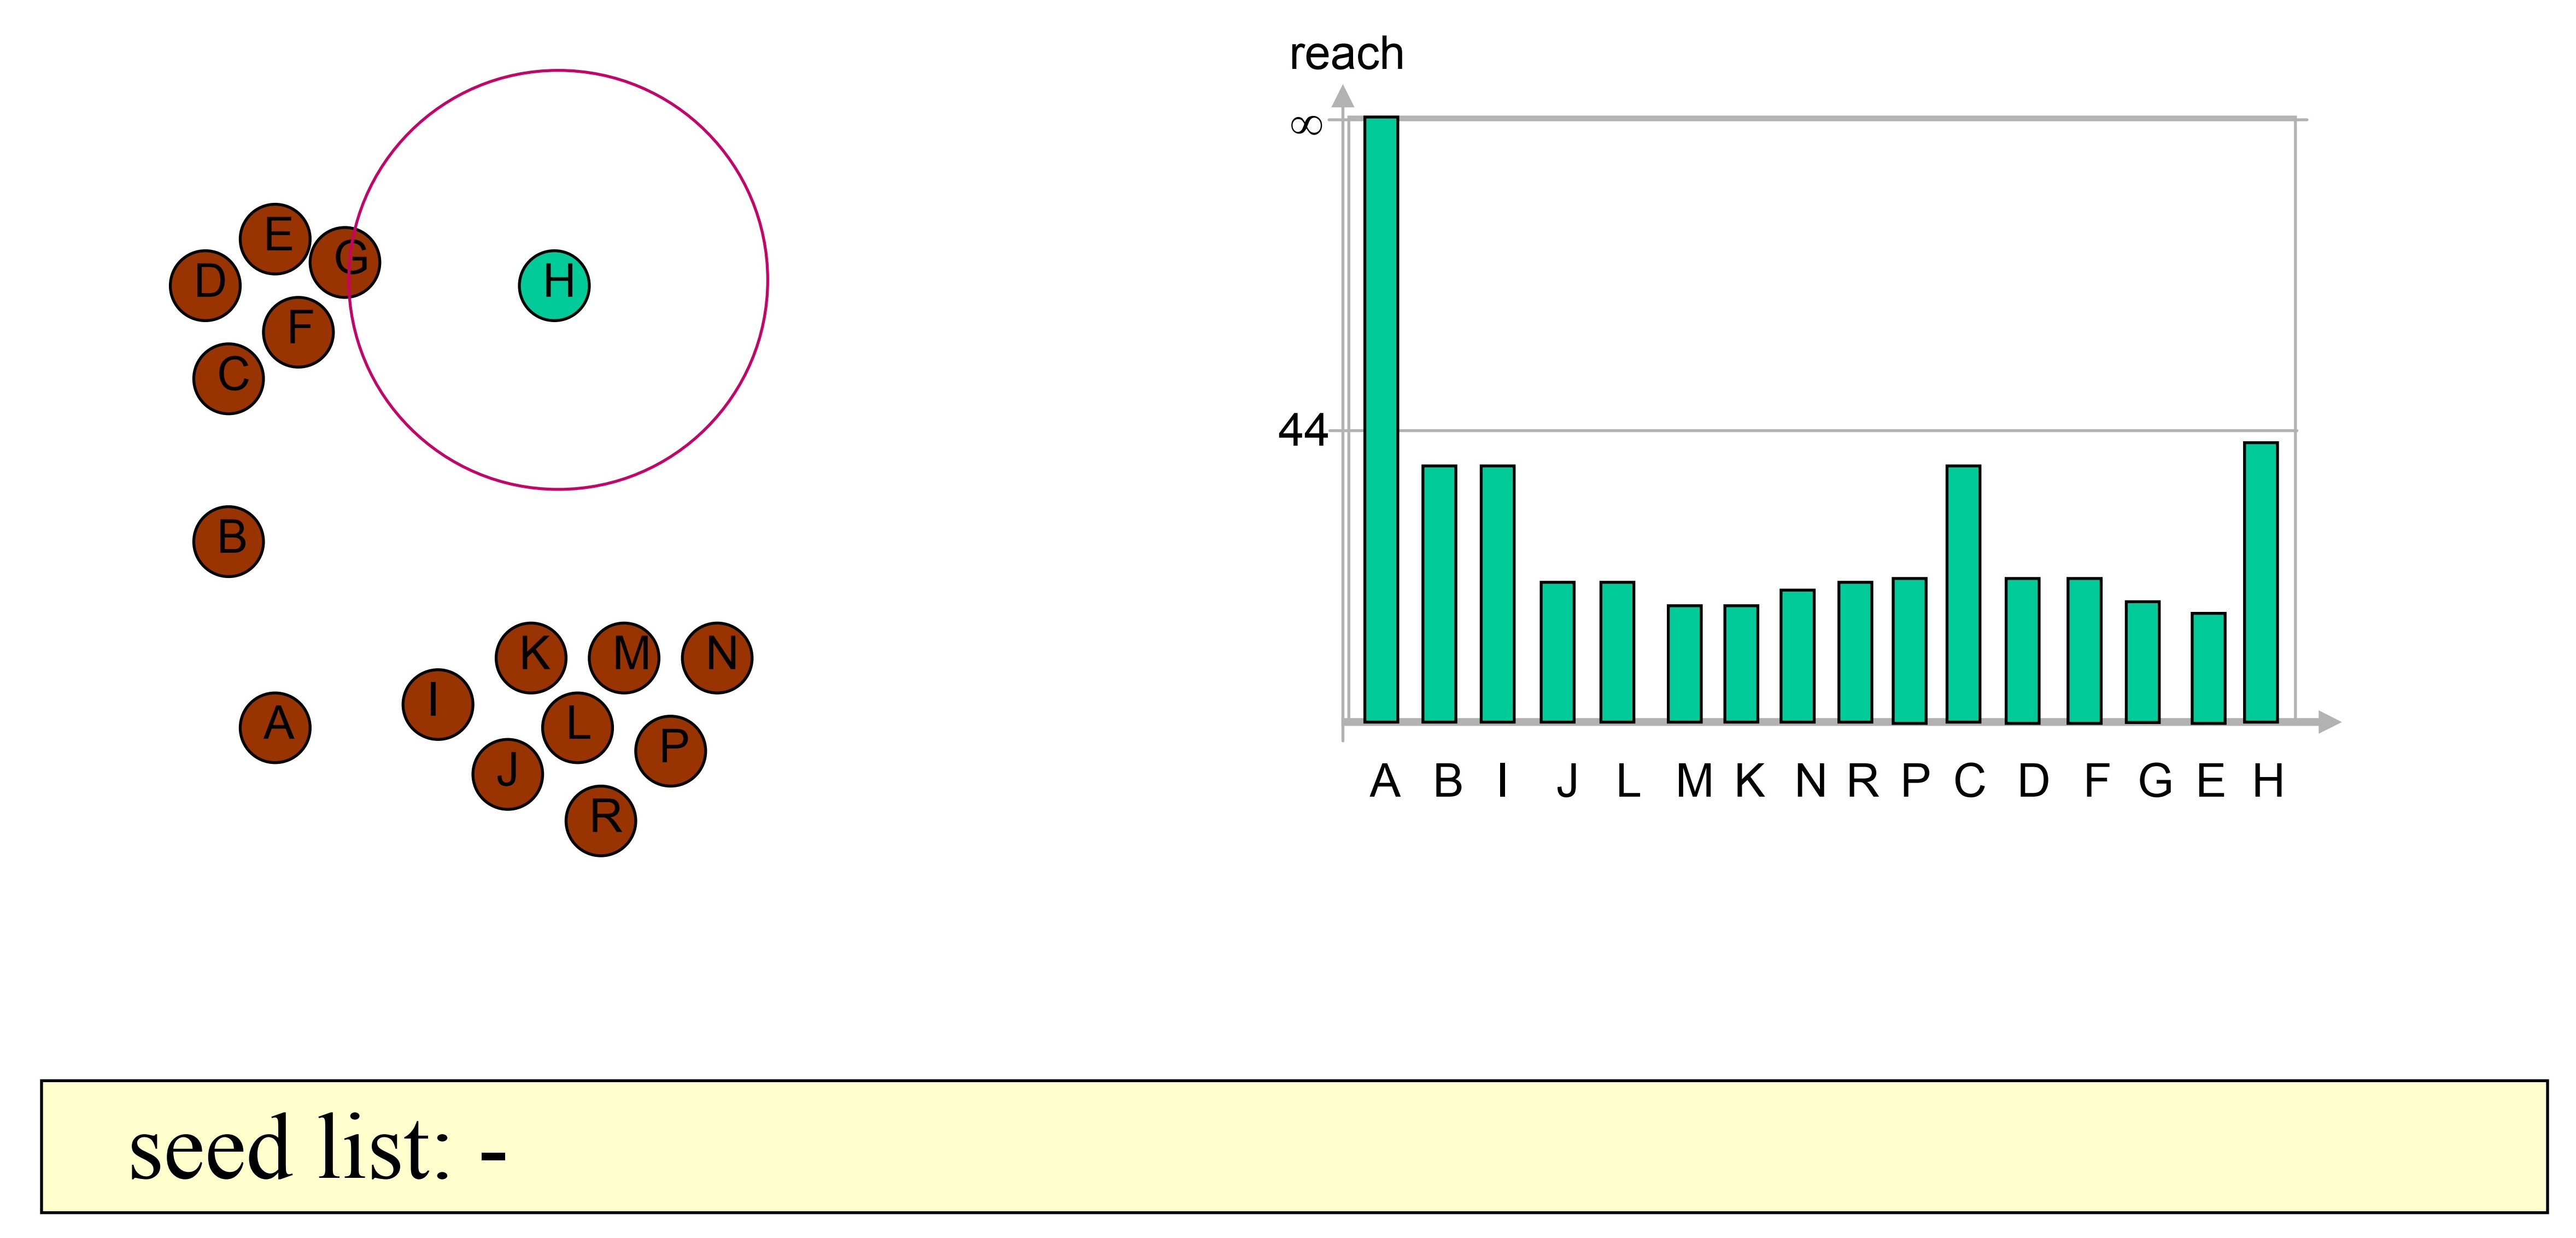
\includegraphics[scale=0.15]{opt7.jpg}
\end{figure}
Im Diagramm können nun Cluster und Subcluster verschiedener Dichte, also verschiedener Erreichbarkeitsdistanzniveaus abgelesen oder algorithmisch extrahiert werden. Dazu werden Teilsequenzen gesucht, welche in einem Gebiet steil abfallender Erreichbarkeitsdistanzen beginnen und in einem Gebiet steil ansteigender Erreichbarkeitsdistanzen enden, sodass der Endpunkt in etwa die gleiche Erreichbarkeitsdistanz besitzt, wie der Startpunkt. Enthält die Teilsequenz mindestens $minPts$-viele Punkte, so kann sie als Cluster interpretiert werden. 
\begin{figure}[H]
\centering
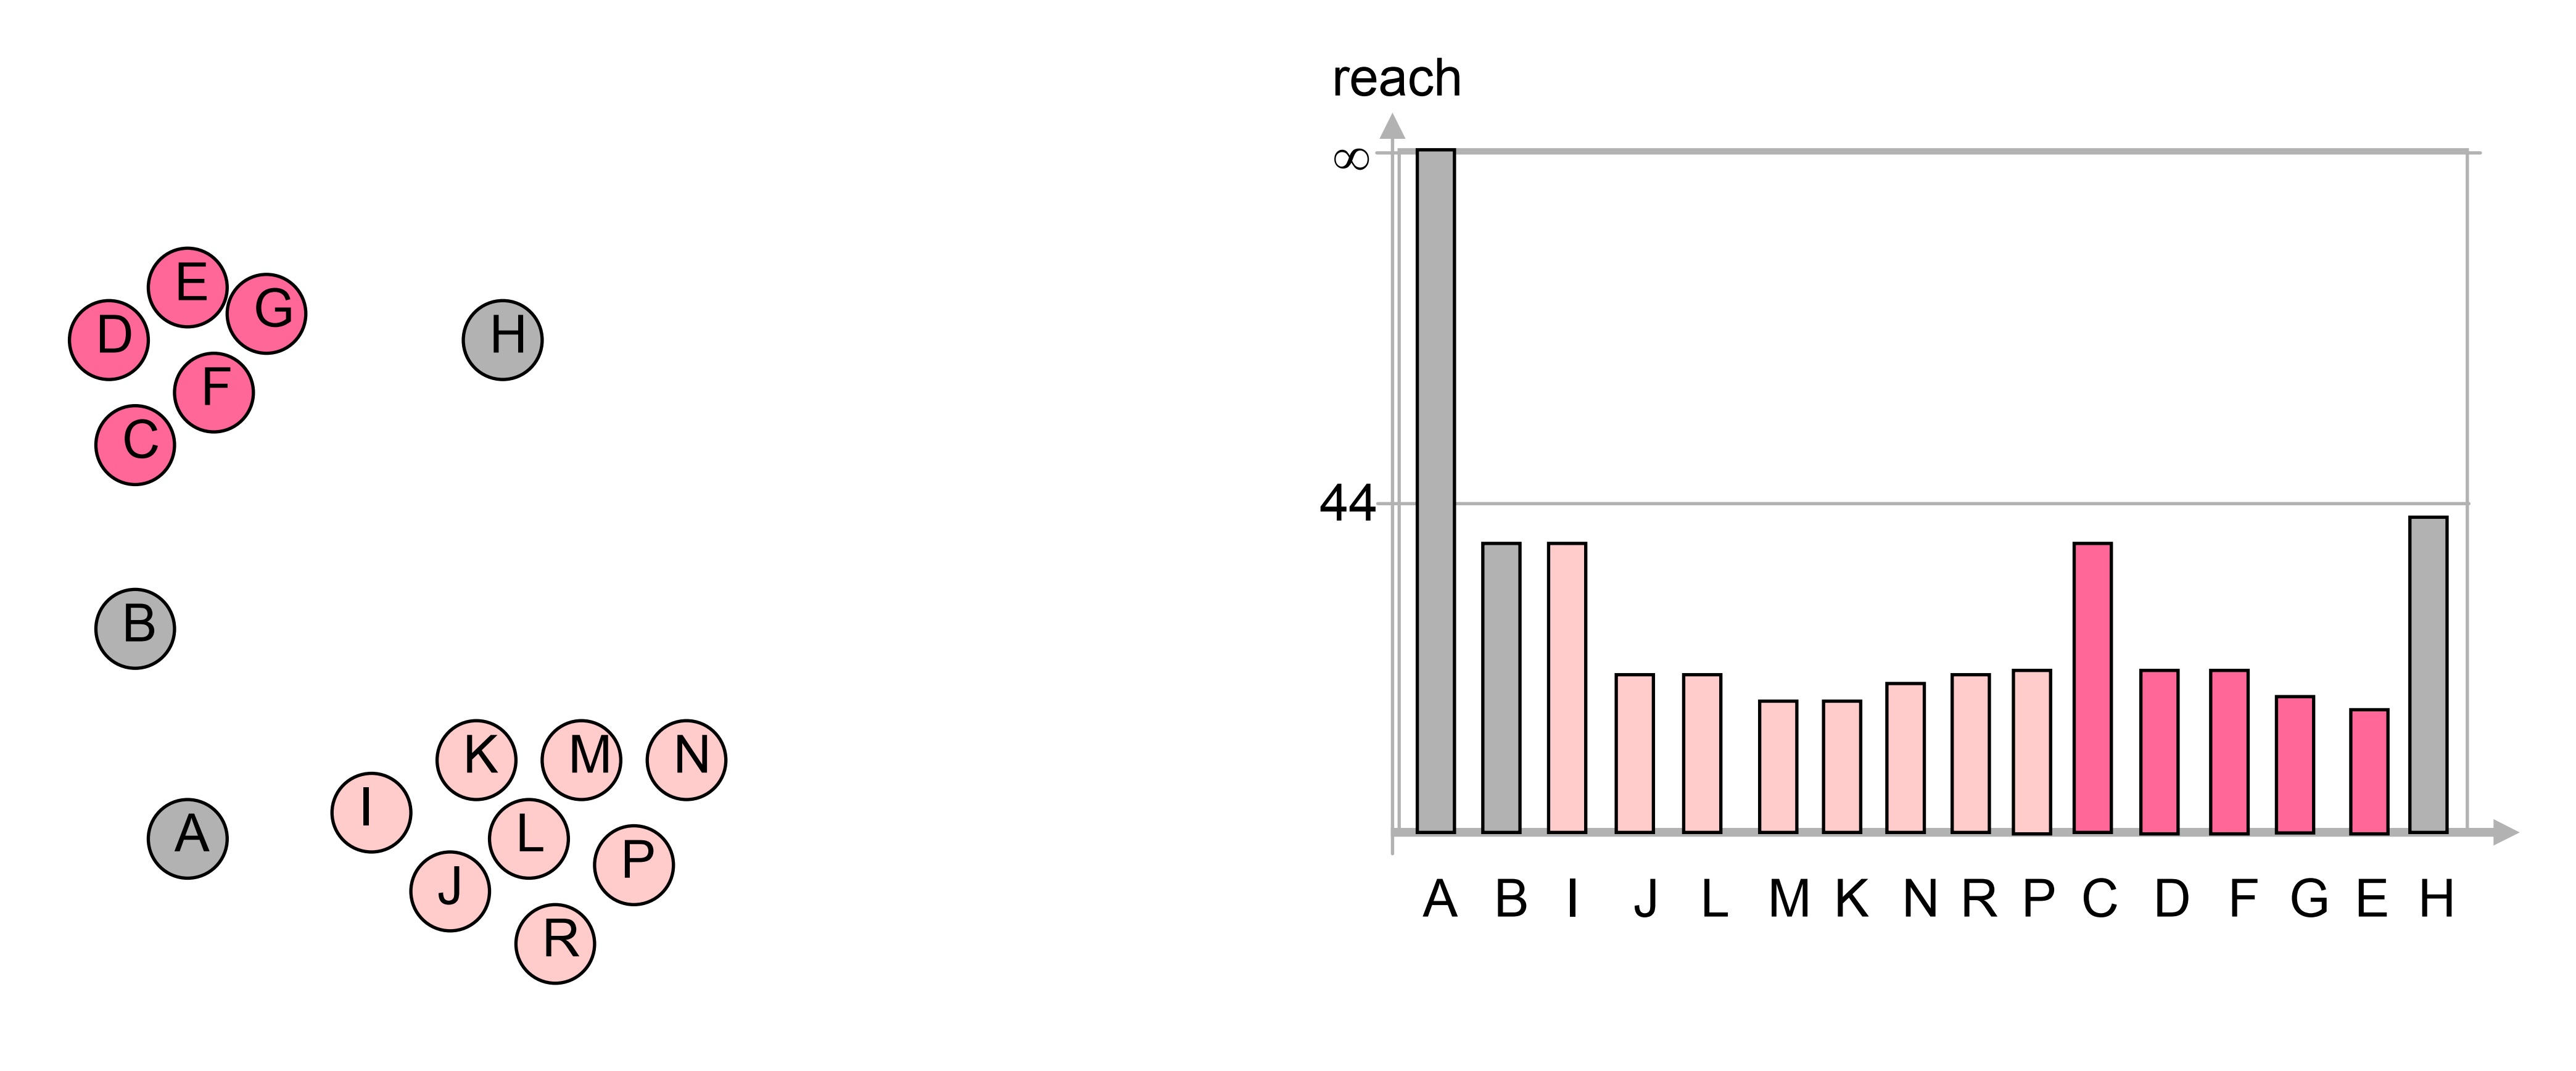
\includegraphics[scale=0.15]{opt8.jpg}
\end{figure}

\subsubsection{Wahl der Parameter $\epsilon$ und $minPts$}
Die Wahl der Parameter $\epsilon$ und $minPts$ sollte so erfolgen, dass die Cluster im Diagramm vertikal zentriert sind. Es dürfen also nur wenige Erreichbarkeitsdistanzen $\infty$ sein. Außerdem darf die Varianz der Erreichbarkeitsdistanzen zwischen zwei benachbarten Punkten nicht zu groß werden. Um dies zu garantieren, wird $\epsilon$ entweder so gewählt, dass die $minPts$-Eigenschaft bezüglich einer kleinen Punktestichprobe immer erfüllt ist oder es wird die durchschnittliche $minPts$-Distanz berechnet. Es wird also diejenige $\epsilon$-Distanz gewählt, die im Durchschnitt von allen Punkten aus $minPts$-viele Punkte einschließt. Der Wert für $minPts$ muss in Abhängigkeit der Größe des Datensatzes gewählt werden. Je feiner die Auflösung der Datenbank, desto größer muss der Wert sein.

\subsubsection{Anwendungsgebiete}
Die Werkzeugreferenz von \textbf{ArcGIS Pro}\footnote{\url{https://pro.arcgis.com/de/pro-app/tool-reference/spatial-statistics/how-density-based-clustering-works.htm}} gibt folgende Anwendungsszenarien für das Werkzeug \textit{Dichte-basierte Clusterbildung} an:

\begin{itemize}
\item Clustering von Rohrbrüchen und Rissen städtischer Wasserversorgungssysteme kann auf bevorstehende Probleme hinweisen. Je nach Größe und Dichte eines Clusters können Gefahrenpotentiale abgeschätzt und vorbeugende Maßnahmen getroffen werden.
\item Positionsdaten von erfolgreichen und nicht erfolgreichen Sportlern z.B. Torschützen beim Fußball clustern, um Muster zu erkennen und daraus neue Spielstrategien ableiten zu können.
\item Angenommen es liegt ein Datensatz vor, der für ein begrenztes Untersuchungsgebiet (z.B. für eine Stadt) aufführt, ob ein Haushalt unter Schädlingsbefall leidet oder nicht. Mittels Clusterbildung können die größten und dichtesten Cluster betroffener Haushaltsgruppen identifiziert und behandelt werden. Dies steigert die Effizienz der Schädlingsbekämpfung.
\item Das Verorten von Tweets infolge von Naturgefahren oder Terroranschlägen kann geclustert und notwendige Rettungsmaßnahmen und Evakuierungen können basierend auf der Größe und Position des identifizierten Clusters vermittelt werden.
\end{itemize}


\subsection{Outlier Detection - Local Outlier Factor}
Ein Problem der dichtebasierten Clusteringverfahren ist, dass manche Punkte entweder als Outlier oder als Clusterpunkt markiert werden. Manchmal möchte man jedoch aus analytischen Gründen selbständig beurteilen und steuern können, was als Outlier markiert werden soll. Aus diesem Grund wurde der Local Outlier Factor (LOF) erfunden, welcher für einen Punkt den Grad seiner Zuordenbarkeit berechnet \cite{lof}.

\subsubsection{Grundbegriffe}
Die $k$-Distanz eines Punktes $p$ ist der Radius $kd(p)$, für den mindestens $k$ Punkte innerhalb oder auf ihm liegen müssen, aber maximal $k-1$ Punkte innerhalb liegen dürfen. \\

Die $k$-Distanz-Nachbarschaft $N_{kd(p)} (p)$ ist die Menge aller Punkte, die maximal den Abstand $kd(p)$ von $p$ haben.

Die Erreichbarkeitsdistanz $rd(o,p)$ ist die $k$-Distanz von $p$, aber mindestens der Abstand $dist(p,o)$.

\subsubsection{Berechnung von LOF}

Zuerst wird die lokale Erreichbarkeitsdichte eines Punktes $p$ berechnet. Diese entspricht dem Kehrwert der durchschnittlichen Erreichbarkeitsdistanzen von den Nachbarn aus:

$$Ird_{minPts}(p) = \left(\frac{\sum\limits_{o \in N_{minPts}(p)} rd_{minPts}(p,o)}{|N_{minPts}(p)|}\right)^{-1}$$

Je höher der Wert, desto besser ist $p$ von seinen Nachbarn aus erreichbar. Die Wahrscheinlichkeit, dass $p$ ein Outlier ist, sinkt.

Auch die lokalen Erreichbarkeitsdichten der Nachbarn von $p$ müssen mit einfließen, um beurteilen zu können, wie gut die Erreichbarkeit von $p$ im Verhältnis zu seiner Nachbarschaft ist. Sind die Nachbarn viel besser zu erreichen als $p$, dann ist $p$ ein starker Outlier:

$$LOF_{minPts}(p) = \frac{\sum\limits_{o \in N_{minPts}(p)}\frac{Ird_{minPts}(o)}{Ird_{minPts}(p)}}{|N_{minPts}(p)|}$$

Ist der Wert von $LOF$ in etwa $1$, handelt es sich bei dem betrachteten Objekt um einen durchschnittlich ähnlich gut erreichbaren Punkt (im Vergleich zu seinen Nachbarn) und somit um einen Clusterpunkt. Für Werte, die größer als $1$ sind, ist der Punkt schlechter erreichbar als seine Nachbarn und somit ein Outlier.

\subsection{Lineare Separation - Support Vector Machine}
Die Support Vector Machine ist ein Klassifikator für linear und nichtlinear separierbare Daten. Er kommt in Geoinformationssystemen häufig zum Einsatz, da er besonders robust gegenüber Rauschen und Variabilität raumbezogener Daten ist \cite{svmingeo}.

Die Grundidee der SVM ist es, ähnlich der Klassifikatoren neuronaler Netze eine optimal separierende Hyperebene zu finden. Ist der Datensatz nicht linear separierbar, so kann er mittels Kernelfunktion in einen Raum transformiert werden, für den eine linear separierende Hyperebene gefunden werden kann \cite{svm}. \\

Im Folgenden wird anhand eines Beispiels der zweidimensionalen Fall zur Berechnung der optimal separierenden Gerade erklärt.

\begin{minipage}{0.4\textwidth}\raggedright
Seien die roten und grünen Punkte in der Abbildung rechts die Objekte, welche den Klassen rot und grün zugehörig sind. Die Herausforderung ist es, die Parameter der Gerade $H_0$ (y-Achsenabschnitt und Steigung) so zu bestimmen, dass der Abstand zu den Randpunkten der beiden Klassen maximal wird. Zur Vereinfachung werden zwei weitere Geraden durch die Randpunkte beider Klassen gelegt. Diese Geraden ($H_1$ und $H_2$) stehen parallel zueinander. Die optimal separierende Gerade ist dann der Median beider Randgeraden.
\end{minipage}
\hfill
\begin{minipage}{0.5\textwidth}
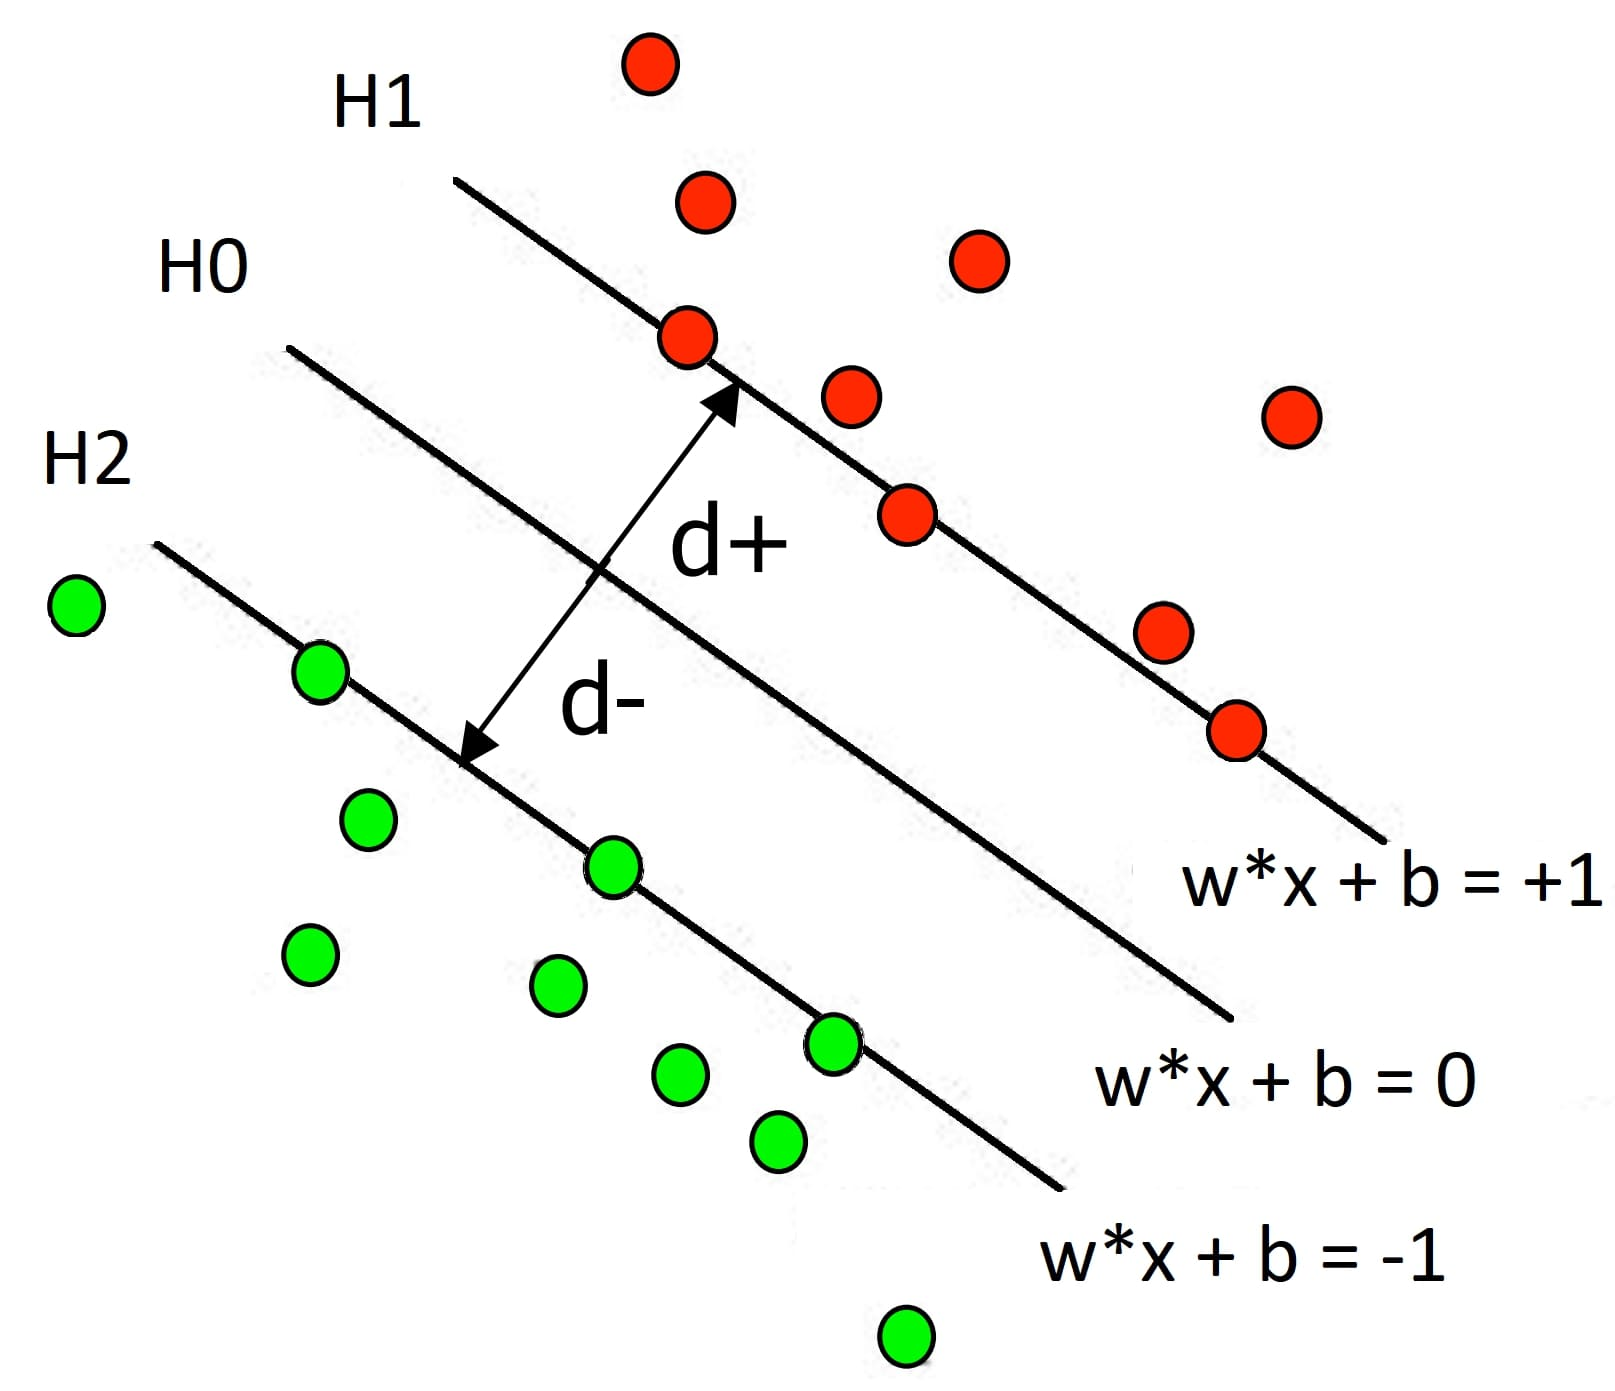
\includegraphics[width=\linewidth]{svm.jpg}
\end{minipage}

Die Klassenlabels der Punkte oberhalb der Geraden $H_1$ sind $y_+ = +1$ und $y_- = -1$ unterhalb der Geraden $H_2$. Sie sind also ein Teil ihrer Koordinate. Dies funktioniert, da sich die y-Werte für das Einsetzen der Punkte $x_+$ und $x_-$ in die Geradengleichung von $H_0$ mithilfe der Signumfunktion transformieren lassen. Gilt für einen Punkt $x_i$, dass $\omega \cdot x_i + b \geqslant 0$, dann gehört dieser zur Klasse rot. Es gilt gleichzeitig für alle Werte $H_0(x_i) \geqslant 0$, dass $sign(H_0(x_i)) = +1 = y_i$.

Setzt man die Labels in die Geradengleichungen der Geraden $H_1$ und $H_2$ ein, so erhält man die Ungleichungen
\begin{equation} \label{hplus}
\omega \cdot x_i +b \geqslant +1
\end{equation}
und 
\begin{equation} \label{hminus}
\omega \cdot x_i +b \leqslant -1
\end{equation}
Für Punkte auf Gerade $H_0$ hingegen gilt 

$$\omega \cdot x_i +b = 0$$

Der Abstand zwischen Randpunkten $x_i$ und der optimal separierenden Gerade kann wie folgt berechnet werden: Der Abstand eines Punktes $(x_0, y_0)$ von einer Geraden $A \cdot x + B \cdot y + C = 0$ beträgt
  
$$\frac{A \cdot x_0 + B \cdot y_0 +C}{\sqrt{A^2 + B^2}}$$

Setzt man für den Punkt einen Randpunkt und für die Gerade die Gleichung von $H_0$, so ergibt sich 

$$\frac{\omega \cdot x_+ +b}{||\omega||}$$

Da $x_+$ auf $H_1$ liegt, gilt $\omega \cdot x_+ +b = 1$ und somit beträgt der Abstand zwischen $x_+$ und $H_0$ 

$$d+ = \frac{1}{||\omega||}$$

Wenn $\frac{1}{||\omega||}$ maximiert wird, dann muss $||\omega||$ minimiert werden. Zur Vereinfachung der Ableitung kann man auch $\frac{1}{2} \cdot ||\omega||^2$ schreiben. Anschließend wird die Lagrange-Funktion aufgestellt. Unter der Voraussetzung, dass zwischen $H_1$ und $H_2$ keine Punkte liegen, kann man die Gleichungen \eqref{hplus} und \eqref{hminus} zusammenfassen:
\begin{equation}
y_i \cdot (\omega \cdot x_i + b) \geqslant 1
\end{equation}

Unter dieser Nebenbedingung lautet die Lagrange-Funktion:
\begin{equation} \label{lagrange}
\mathcal{L}(\vec{\omega},b,\vec{\alpha}) = \frac{1}{2}||\vec{\omega}||^2 - \sum_{i=1}^n \alpha_i \cdot \left[y_i \cdot (\vec{\omega} \cdot \vec{x_i} + b) - 1\right]
\end{equation}

Partielle Ableitungen gleich null setzen:

\begin{equation} \label{Lpw}
\frac{\partial \mathcal{L}}{\partial \vec{\omega}} = 0 \Leftrightarrow \vec{\omega} = \sum_{i=1}^n \alpha_i \cdot y_i \cdot \vec{x_i}
\end{equation}
und
\begin{equation} \label{Lpb}
\frac{\partial \mathcal{L}}{\partial b} = 0 \Leftrightarrow \sum_{i=1}^n \alpha_i \cdot y_i = 0
\end{equation} 

Nach Einsetzen von \eqref{Lpw} in \eqref{lagrange}:

\begin{equation} \label{lagrange2}
\begin{split}
\mathcal{L}(\vec{\omega},b,\vec{\alpha}) = \frac{1}{2}\left(\sum_{i=1}^n \alpha_i \cdot y_i \cdot \vec{x_i}\right)\cdot \left(\sum_{j=1}^n \alpha_j \cdot y_j \vec{x_j}\right) - \left(\sum_{i=1}^n \alpha_i \cdot y_i \cdot \vec{x_i}\right) \cdot \left(\sum_{j=1}^n \alpha_j \cdot y_j \cdot \vec{x_j}\right)\\ - \sum_{i=1}^n \alpha_i \cdot y_i \cdot b + \sum_{i=1}^n \alpha_i
\end{split}
\end{equation}

Nach Einsetzen von \eqref{Lpb} in \eqref{lagrange2} ergibt sich folgende Gleichung:

\begin{equation} \label{lagfinal}
\mathcal{L}(\vec{\omega},b,\vec{\alpha}) = \sum_{i=1}^n \alpha_i - \frac{1}{2} \sum_{i=1}^n \sum_{j=1}^n \alpha_i \cdot \alpha_j \cdot y_i \cdot y_j \frac{\vec{x_i} \cdot \vec{x_j}}{ \langle \vec{x_i},  \vec{x_j} \rangle}
\end{equation}

Diese lässt sich unter Nebenbedingung \eqref{Lpb} und $\alpha_i \geqslant 0$ maximieren.

\vspace*{\fill}

Im Folgenden habe ich einen Optimierer (scipy.optimize.minimize) zur Maximierung von \eqref{lagfinal} für ein selbstgewähltes Beispiel konkret in Python implementiert. Die Maximierung von $\mathcal{L}$ entspricht der Minimierung von $-\mathcal{L}$:


\begin{figure}[H]
\centering
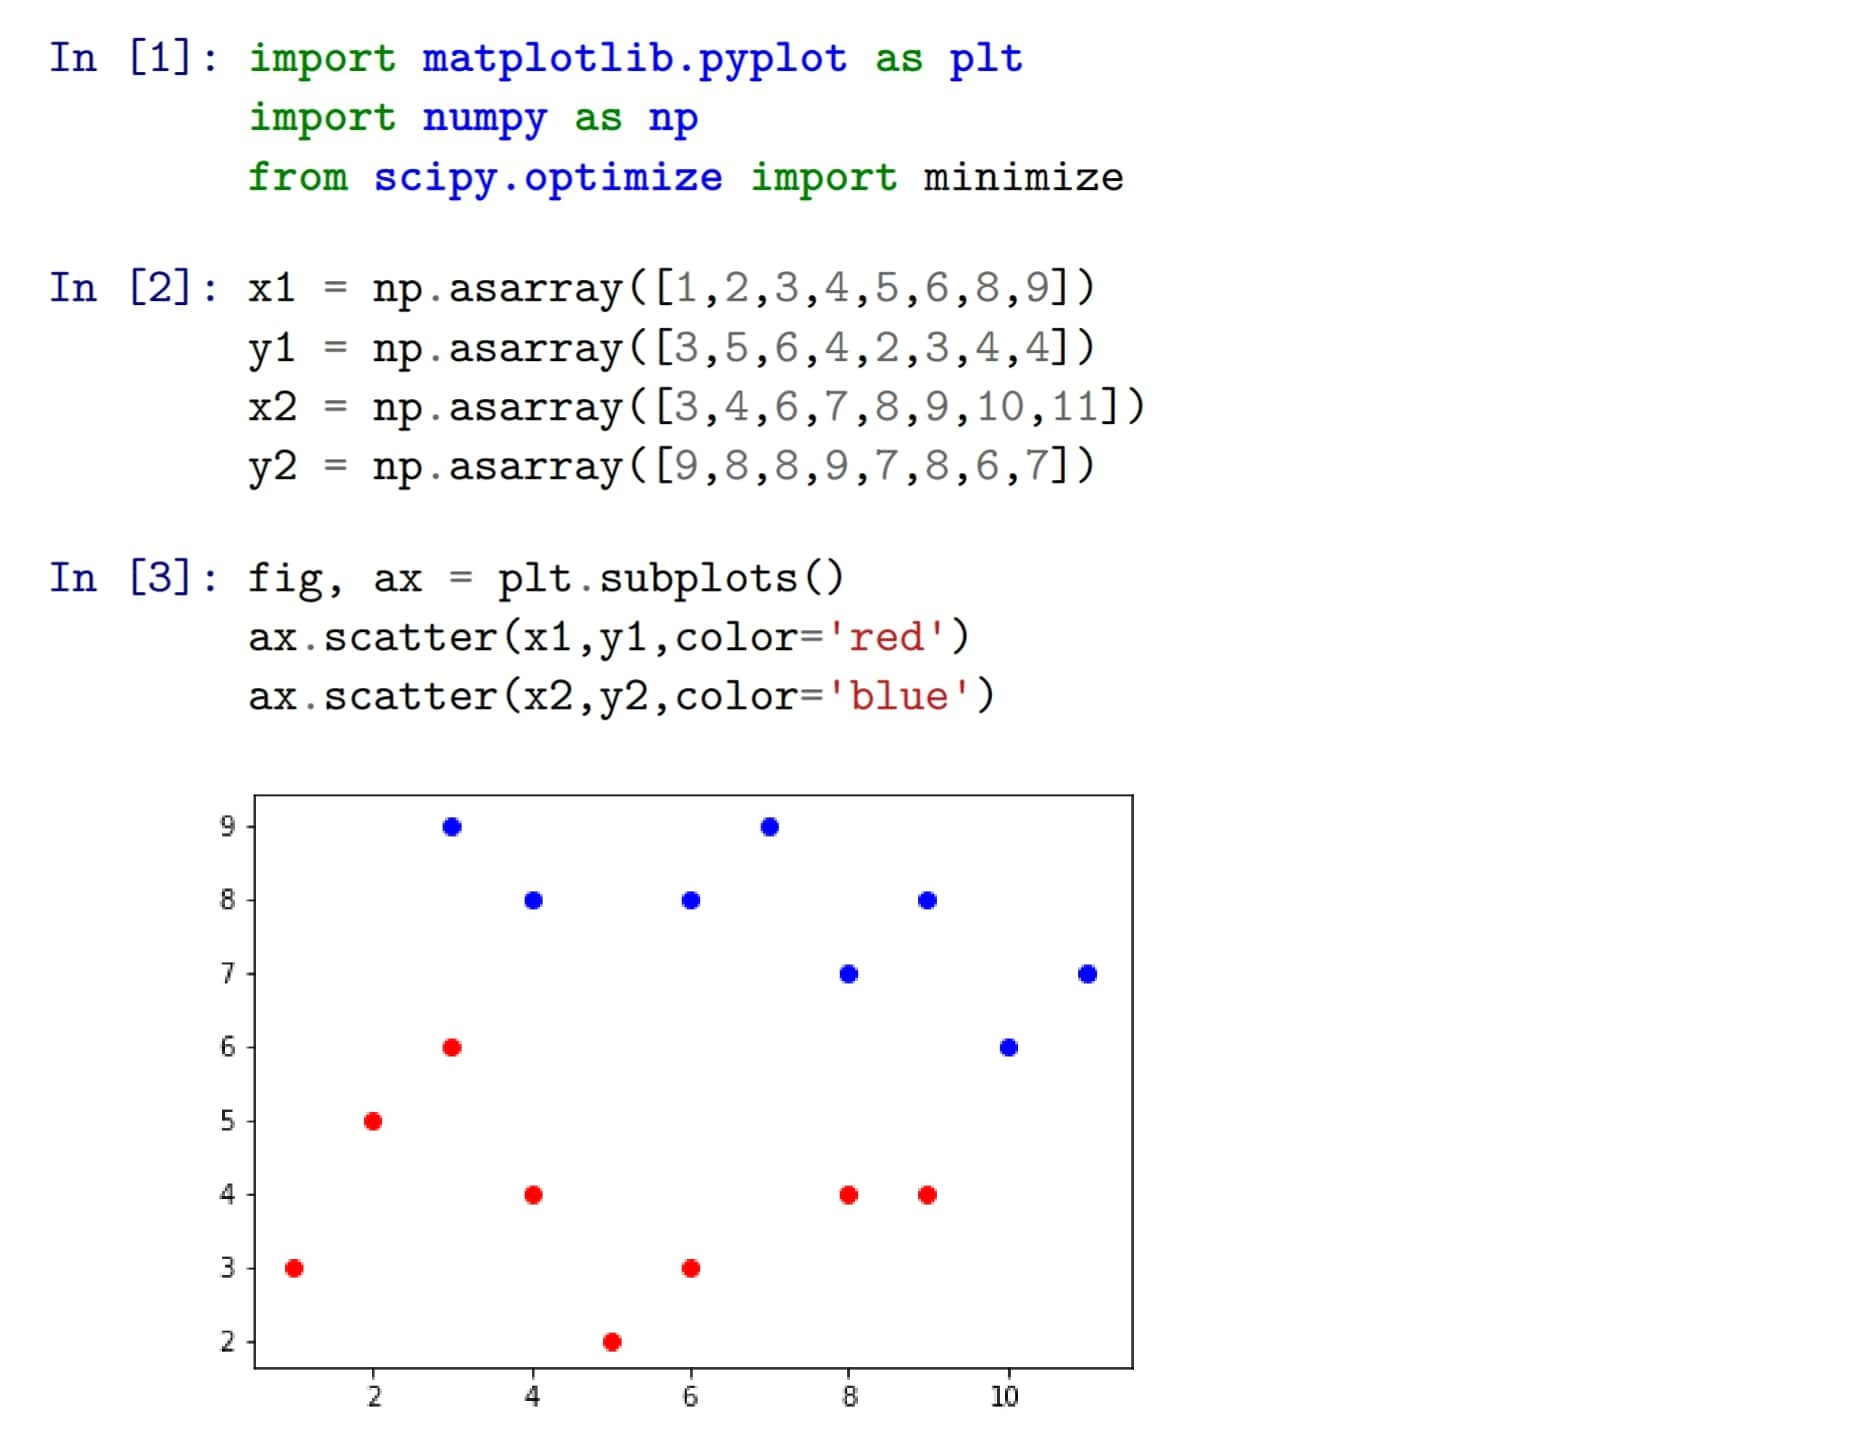
\includegraphics[scale=0.43]{svm1.jpg}
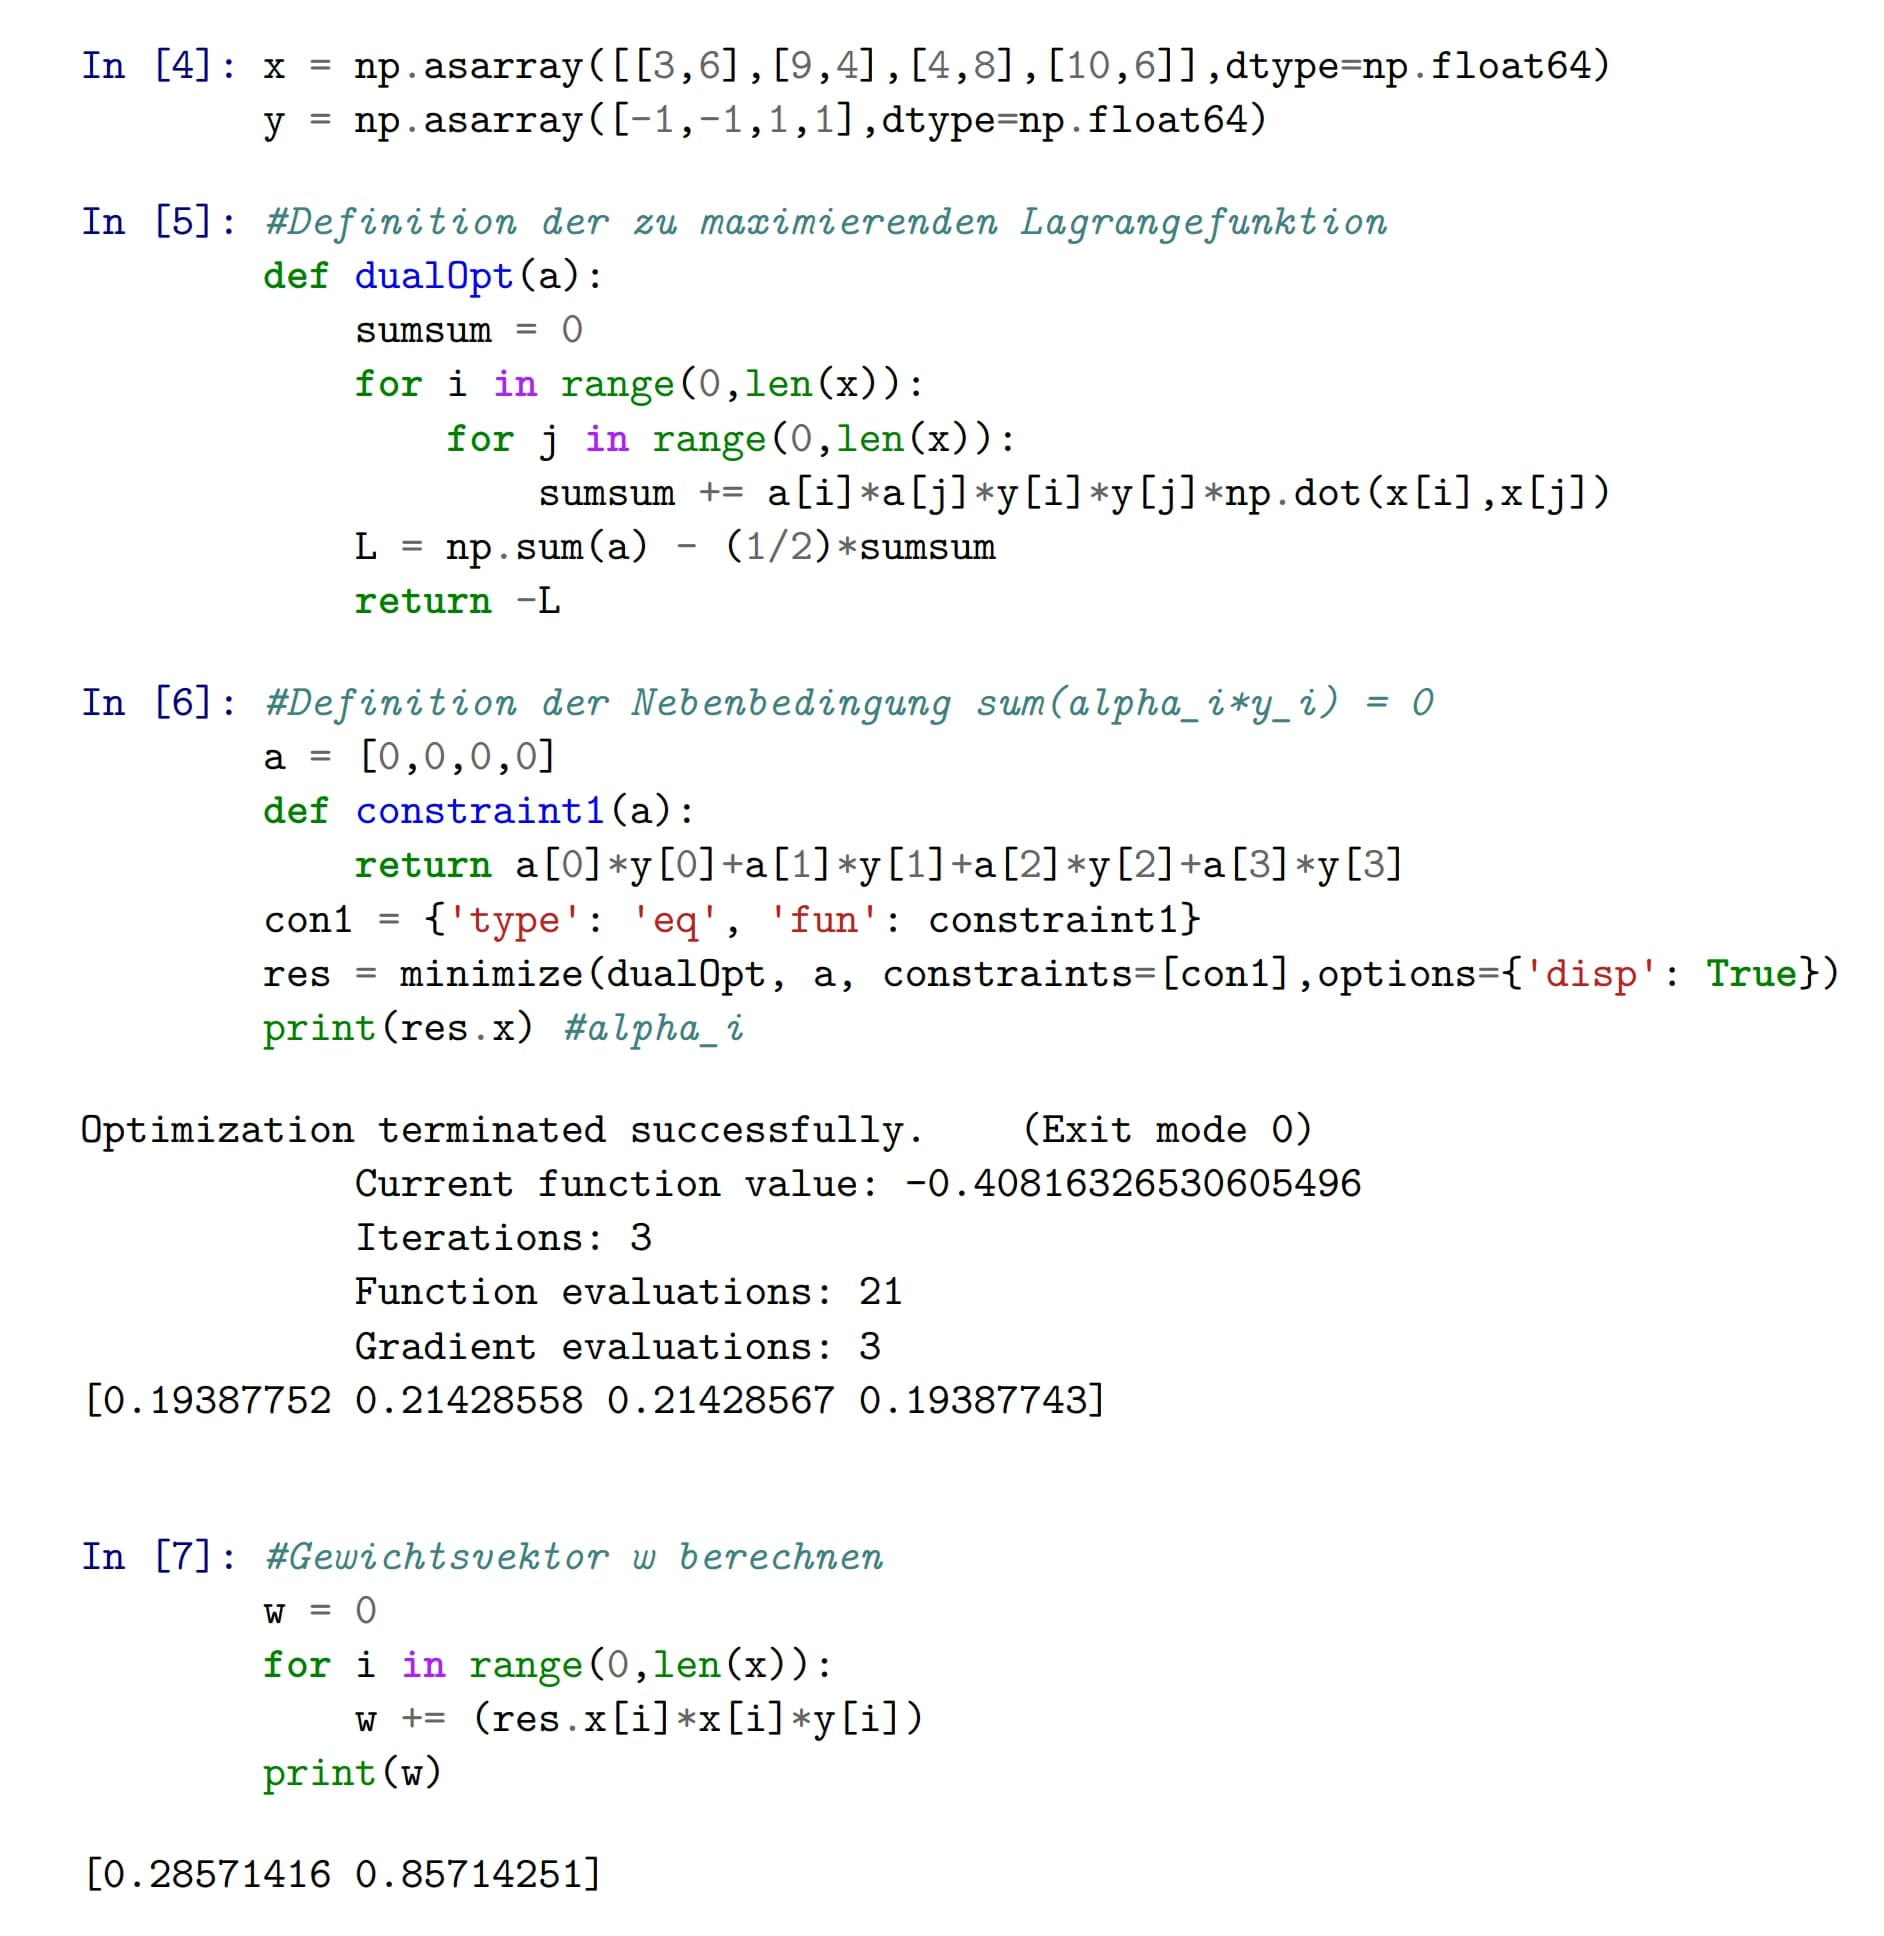
\includegraphics[scale=0.45]{svm2.jpg}
\end{figure}
\begin{figure}[H]
\centering
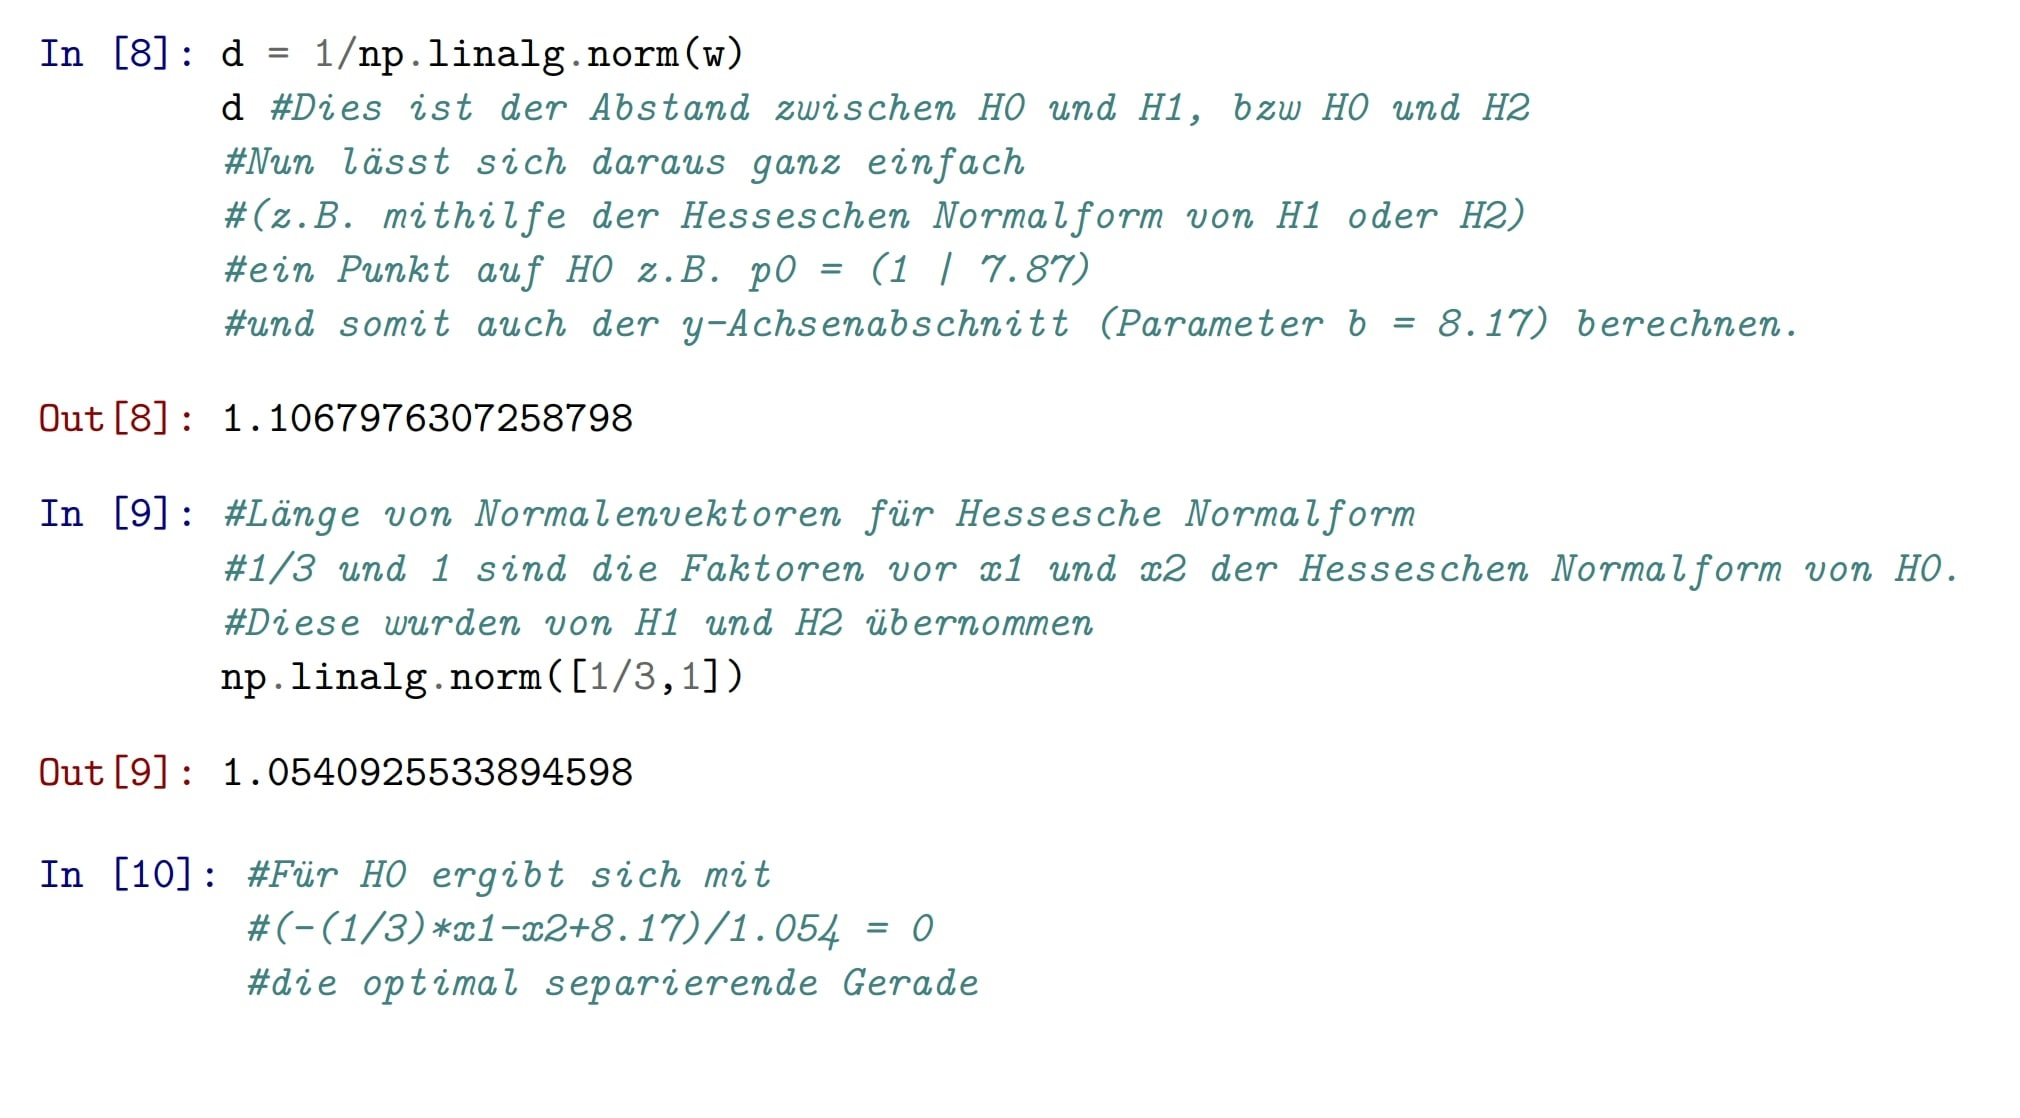
\includegraphics[scale=0.47]{svm3.jpg}
\end{figure}

\hfill

\section{Fuzzy-Clustering}

\subsection{Fuzzy C-Means (FCM)}
Neuere Clusteringverfahren verwenden häufig modifizierte Versionen des FCM(Fuzzy C-Means)-Algorithmus\cite{clustgis}. Dieser berechnet für jeden Punkt den Grad seiner Zuordnung zu allen Clustern. Er gehört zu den probabilistischen, partitionierenden Clusteringverfahren.
Die zu minimierende Kostenfunktion lautet:

$$J_m(X,U,V) = \sum_{i=1}^{c} \sum_{k=1}^{n} u_{ik}^m \cdot d^2(v_i,x_k) \quad \forall i,k \in [0,1]$$

Wobei $u_ik$ die eingangs beschriebene Zugehörigkeitsmatrix ist und $d^2$ ein Abstandsmaß zur Gewichtung der Zugehörigkeit in Abhängigkeit des Abstandes zwischen Punkt $x_k$ und Clusterzentroid $v_i$. Parameter $m>1$ ist die Vagheit der Zerlegung und gibt an, wie stark die Zugehörigkeitsgrade abfallen. In der Regel wird hier der Wert $m=2$ verwendet.
\\
Dabei sind folgende Nebenbedingungen Einzuhalten:
$$\forall k \in {1, \dots, n} : \sum_{i=1}^c u_{ik} = 1$$
Dies sorgt dafür, dass jedes Objekt das Gesamtgewicht $1$ erhält und somit kein Punkt bevorzugt wird.
$$\forall i \in \{1, \dots, c\} : \sum_{i=1}^n u_{ik} > 0$$
Dies garantiert, dass es keinen Cluster gibt, dem nichts zugeordnet wurde. Es muss also mindestens ein Objekt geben, das eine positive Zugehörigkeit zu Cluster $i$ hat.
\\
Zur Optimierung der Zielfunktion, bildet man die partiellen Ableitungen der Lagrangefunktion 
$$\mathcal{L}(X, U, V , \Lambda) = \sum_{i=1}^{c} \sum_{k=1}^{n} u_{ik}^m \cdot d^2(v_i,x_k) + \sum_{k=1}^n \lambda_k \left(\sum_{i=1}^c u_{ik} - 1\right)$$

Man erhält die zu aktualisierenden Werte von Zugehörigkeitsmatrix und Clusterzentroiden:
\begin{equation} \label{uikopt}
u_{ik} = \frac{1}{\sum\limits_{j=1}^c \left(\frac{d^2(v_i, x_k)}{d^2(v_j, x_k)^{\frac{1}{m-1}}}\right)}
\end{equation}
und
\begin{equation} \label{viopt}
v_i = \frac{\sum\limits_{k=1}^n u_{ik}^m \cdot x_k}{\sum\limits_{k=1}^n u_{ik}^m}  \quad \forall i \in \{1, \dots, c\}
\end{equation}


Der Algorithmus zum Finden der besten Clusterzentroide ist wie beim k-means Verfahren ein alternierendes Programm.
%http://tug.ctan.org/macros/latex/contrib/algorithmicx/algorithmicx.pdf <- für Syntax!
\begin{algorithm}[H]
\caption{$FCM(X,c,m,\epsilon)$}\label{fcm}
\begin{algorithmic}[1]
\Require{$X$ ist ein $d$-dimensionaler Datensatz mit $n$ Datenpunkten, $2 \leqslant
c \leqslant n$ ist die Clusteranzahl, $m > 1$ ist  die Vagheit und $ \epsilon > 0$ ist die Terminierungsgenauigkeit}
\State Initialisiere die Clusterprototypen $v' = \{v'_1, \dots, v'_c\}$
\State $v = \emptyset$
\Repeat
\State $v=v'$
\State Berechne die Zugehörigkeitsgrade $u_{ik}$ von jedem Datenpunkt $x_k$ zu jedem Cluster $C_i$ nach \hspace*{5mm} Formel \eqref{uikopt} \textit{// Schritt 1}
\State Berechne die neuen Clusterprototypen $v' = \{v'_1, \dots, v'_c\}$ nach Formel \eqref{viopt} \textit{// Schritt 2}
\Until{$||v - v'|| < \epsilon$}
\State \Return $v'$
\end{algorithmic}
\end{algorithm}

Leider hat das ursprüngliche FCM-Verfahren viele Nachteile. Man weiß leider nie, ob ein lokales oder ein globales Minimum für die Kostenfunktion gefunden wurde. Je nach Initialisierungsmethode muss FCM unter Umständen mehrmals mit unterschiedlichen Parametern ausgeführt werden, um das beste Ergebnis zu finden. Wird für das Distanzmaß die euklidische Distanzfunktion verwendet, können nur gleich große, sphärische Cluster gefunden werden. Aus diesem Grund wurden viele weitere Fuzzy-Clusteringalgorithmen entwickelt, die auf dem gleichen Grundprinzip basieren, jedoch andere Kostenfunktionen minimieren.
\\
Da die Zugehörigkeiten der Datenobjekte relativ sind, können Outlier fälschlicherweise überberücksichtigt werden:

\begin{figure}[H]
\centering
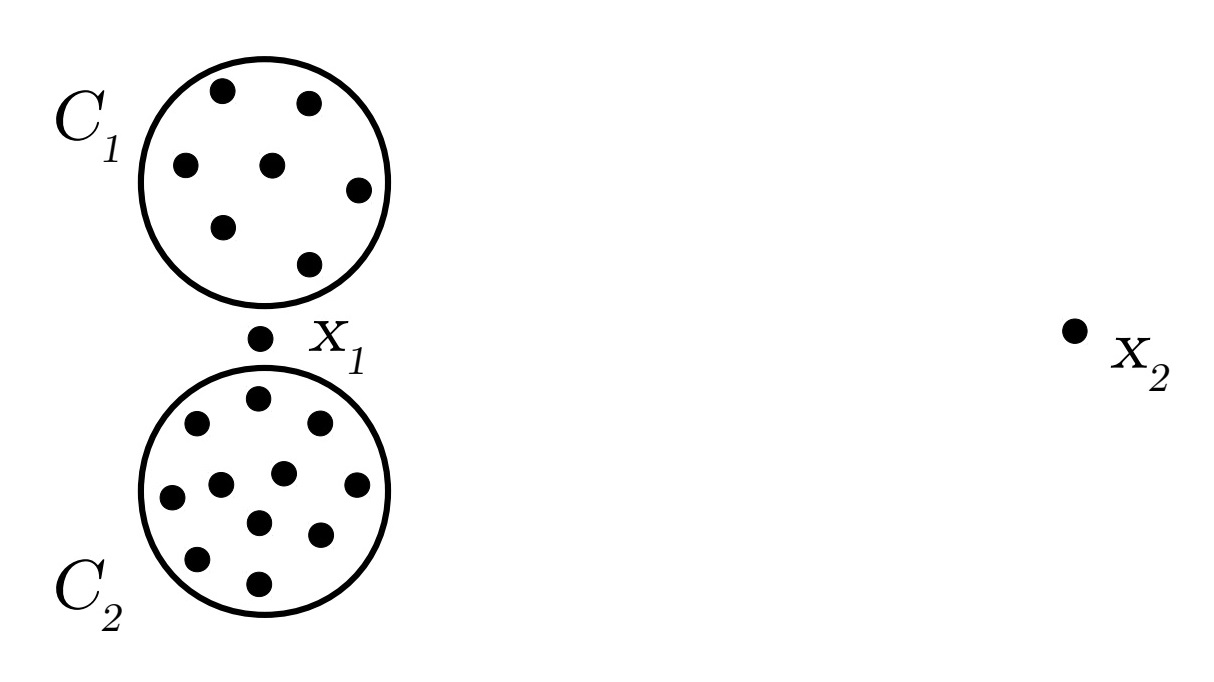
\includegraphics[scale=0.35]{fcmnachteil.jpg}
 \caption{Punkt $X_1$ hat den gleichen Zugehörigkeitsgrad wie der Outlier $X_2$}
\end{figure}
~\\
Im Anhang wird FCM ab Zeile 9 anhand eines Beispiels demonstriert.

\subsection{Possibilistic C-Means (PCM)}
Eine Lösung bieten possibilistische Clusteringverfahren. Werden die relativen Zugehörigkeiten $u_{ik}$ durch absolute Ähnlichkeitswerte $t_{ik}$ (typicality values) ersetzt, so fällt die Nebenbedingung $\sum\limits_{i=1}^c u_{ik} = 1$ weg. Die Gesamtzugehörigkeit jedes Datums zu allen Clustern wird also nicht mehr auf alle Cluster verteilt. Stattdessen soll ein Wert zwischen $0$ und $c$ gewählt werden:

$$0 < \sum_{i=1}^c t_{ik} \leqslant c$$

Eine mögliche Lösung für die Kostenfunktion aus FCM mit Ähnlichkeitswerten wäre trivial. Sei $\epsilon>0$: 
$$\forall k \exists i: t_{1k}=0, \dots, t_{i-1k}=0, t_{ik} = \epsilon, t_{i+1k}=0, \dots, t_{ck}=0 $$
Es muss also nur ein einziger Ähnlichkeitswert größer als $0$ sein. Um diese triviale Lösung zu verhindern, führt man einen Bestrafungsterm ein:

$$\sum_{i=1}^c  \gamma_i \sum_{k=1}^n (1-t_{ik})^m, \quad \gamma_i >0$$

Werden die typicality Values zu klein, so wird der Bestrafungsterm immer größer. Der Parameter $\gamma_i$ regelt dabei, wie stark der Einfluss der Bestrafung für den jeweiligen Cluster $C_i$ ausfallen darf. Außerdem beeinflusst er die Wahl von $t_{ik}$ indirekt. So konvergiert $t_{ik}$ für sehr große Werte von $\gamma_i$ gegen den Wert $1$. Entspricht $\gamma_i$ dem Wert der Distanzfunktion $d^2 (v_i,x_k)$, so hat $t_{ik}$ den Wert $\frac{1}{2}$.
\\
Die Kostenfunktion für PCM lautet insgesamt:

$$J_m(T,V,X,\gamma) = \sum_{i=1}^{c} \sum_{k=1}^{n} t_{ik}^m \cdot d^2(v_i,x_k) + \sum_{i=1}^c  \gamma_i \sum_{k=1}^n (1-t_{ik})^m,\quad \gamma_i>0 \forall i$$

Leider führt auch diese Funktion je nach Initialisierung der Clusterprototypen zu einer trivialen Lösung, bei der nur noch ein einziger Cluster erkannt wird. Mögliche Lösungen sind die Initialisierung mit der Ausgabe eines zuvor ausgelösten FCM-Durchlaufs oder das Hinzufügen eines weiteren Bestrafungsterms, der Clusterabstoßung. Je näher sich die Clusterzentroide im Laufe der Optimierung kommen, desto größer soll die Kostenfunktion werden. Gleichzeitig sollen die Punkte nicht nur einem Cluster zugeordnet werden und alle anderen Cluster möglichst weit weg sein. Zwei Abstoßungsfunktionen\cite{cabstossung}, die solche Kriterien erfüllen, sind: $f(x) = \frac{1}{x^2}$ und $g(x) = \frac{1}{e^{x^2}}$.

\begin{figure}[H]
\centering
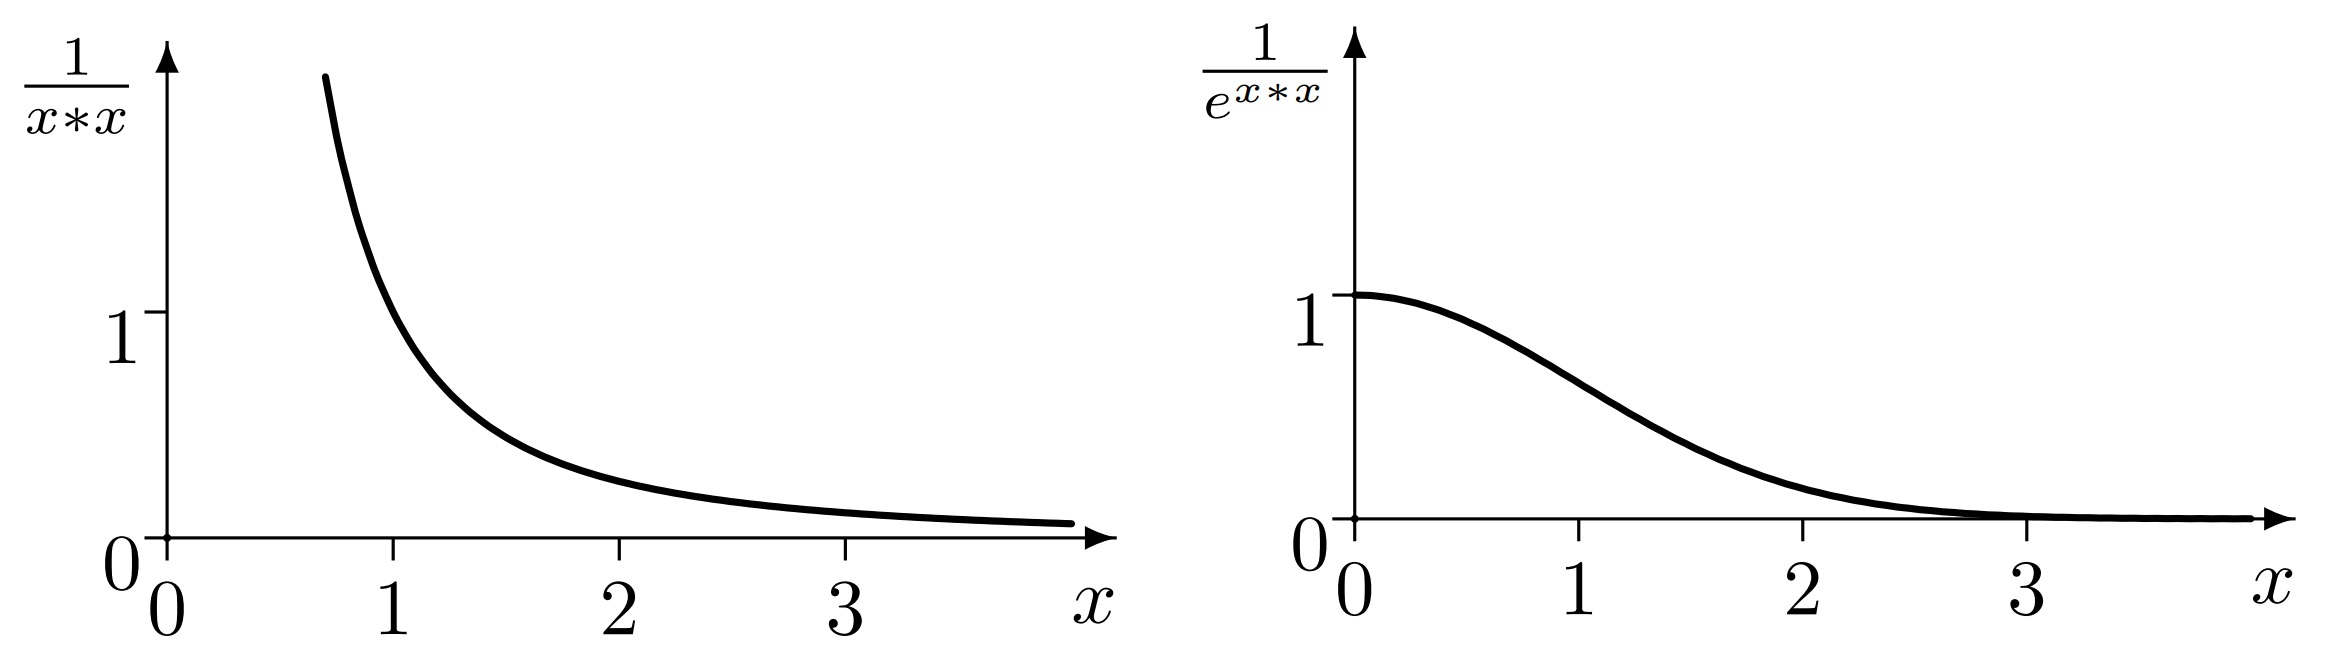
\includegraphics[scale=0.3]{abstossung.jpg}
 \caption{Geeignete Abstoßungsfunktionen: Je größer der Clusterabstand, desto kleiner die Belohnung in der Kostenfunktion}
\end{figure}

$f(x)$ führt zu Kostenfunktion

\begin{equation}
\begin{split}
J_m(T,V,X,\gamma,\eta,\zeta) = \sum_{i=1}^{c} \sum_{k=1}^{n} t_{ik}^m \cdot d^2(v_i,x_k) + \sum_{i=1}^c  \gamma_i \sum_{k=1}^n (1-t_{ik})^m + \\ \sum_{i=1}^c \eta_i \sum_{j=1,j\neq i}^c \frac{1}{\zeta\cdot d^2(v_i,v_j)},\quad \gamma_i>0 \forall i, \zeta\in \mathbb{R_+}
\end{split}
\end{equation}

und $g(x)$ führt zu 

\begin{equation}
\begin{split}
J_m(T,V,X,\gamma,\eta,\zeta) = \sum_{i=1}^{c} \sum_{k=1}^{n} t_{ik}^m \cdot d^2(v_i,x_k) + \sum_{i=1}^c  \gamma_i \sum_{k=1}^n (1-t_{ik})^m + \\ \sum_{i=1}^c \eta_i \sum_{j=1,j\neq i}^c e^{-\zeta\cdot d^2(v_i,v_j)},\quad \gamma_i>0 \forall i, \zeta\in \mathbb{R_+}
\end{split}
\end{equation}

Dabei normiert $\zeta$ den Abstand zwischen je zwei Clusterprototypen und $\eta_i$ setzt den Abstand eines Clusters zu den benachbarten Clustern in Relation zu den Abständen zu Datenpunkten innerhalb des Clusters. Ein clusterspezifisches Abstoßungsmaß ist erforderlich, damit große Cluster nicht stärker berücksichtigt werden, als kleine Cluster.
\\
Nach Minimierung der Kostenfunktion ergeben sich für die Aktualisierungen der Ähnlichkeitswerte $t_{ik}$ und Clusterzentroide $v_i$ folgende Formeln:

$$t_{ik} = \frac{1}{1+\left(\frac{d^2(v_i,x_k)}{\gamma_i}\right)^{\frac{1}{m-1}}},\quad 1\leqslant i \leqslant c, 1\leqslant k\leqslant n$$
und
$$v_i = \frac{\sum\limits_{k=1}^n t_{ik}^m x_k - \eta_i \zeta \sum\limits_{j=1,j\neq i}^c v_j e^{-\zeta d^2(v_j,v_i)}}{\sum\limits_{k=1}^n t_{ik}^m x_k - \eta_i \zeta \sum\limits_{j=1,j\neq i}^c e^{-\zeta d^2(v_j,v_i)}},\quad 1\leqslant i \leqslant c$$
und $\gamma_i$ wird auf die intra-cluster Distanz gesetzt:
$$\gamma_i = K\cdot \frac{\sum\limits_{k=1}^n u_{ik}^m d^2 (x_k, v_i)}{\sum\limits_{k=1}^n u_{ik}^m},\quad K>0$$

\subsection{Possibilistic Fuzzy C-Means (PFCM)}
Eine erweiterte Kombination aus den FCM und PCM Algorithmen kommt ganz ohne Clusterabstoßung aus und verhindert, dass die absoluten Zugehörigkeitsgrade bei großen Datensätzen zu klein werden und ihre Aussagekraft verlieren. Die Zielfunktion von PFCM \cite{pfcmpaper} lautet:

\begin{equation}
\begin{split}
J_{m,\eta}(U,T,V,X,\gamma) = \sum_{i=1}^{c} \sum_{k=1}^{n} \left(a\cdot u_{ik}^m + b\cdot t_{ik}^{\eta}\right)\cdot d^2(v_i,x_k) + \sum_{i=1}^c  \gamma_i \sum_{k=1}^n (1-t_{ik})^{\eta}, \\ m>1, n>1,a>0, b>0, 0\leqslant u_{ik}, t_{ik} \leqslant 1
\end{split}
\end{equation}

Dabei steuern $a$ und $b$ den relativen Einfluss der verschiedenen Arten von Zugehörigkeitsgraden. Je ungeeigneter die Ähnlichkeitswerte ($t_ik$) in Anbetracht der Größe des Datensatzes sind, desto stärker wird die Gewichtung der Zugehörigkeitsgrade ($u_{ik}$). Mit $a=0$ wird PFCM zu PCM und mit $b=0$ zu FCM.
\\~\\
Im Anhang wird PFCM ab Zeile 12 anhand eines Beispiels demonstriert.

\subsection{Scale Space Filter Clustering}
Eine weitere Variante des FCM-Algorithmus, der Selective Scale Space based FCM \cite{scalespacefcm}, wurde entworfen, um die Gruppierung raumbezogener Daten zu verbessern. \\

In einer Menge von Objekten kann es vorkommen, dass sich bestimmte Objektfeatures nicht clustern lassen. Dies ist der Fall, wenn sich die Werte eines Featurevektors zu ähnlich sind und keine deutlichen Cluster bilden. Man sagt, dass die Cluster nicht linear separabel sind. Der Scale Space Filter löst dieses Problem, indem er mithilfe einer Transformationsvorschrift nahe beieinander liegende Punkte weiter zusammen schiebt und weiter entfernte Punkte voneinander abstößt. Wird der Filter jedoch auf bereits für das Clustering geeignete Parameter angewandt, kann der Informationsgehalt verschlechtert werden. Aus diesem Grund müssen zuerst diejenigen Features selektiert werden, welche das Potential haben, nach ihrer Transformation die Clusteringgenauigkeit zu verbessern. Ein weiterer Vorteil des Selektionsprozesses ist die Optimierung der Laufzeiteffizienz. Ein Parameter ist genau dann geeignet, wenn seine Standardabweichung einen bestimmten Schwellwert unterschreitet.
\\
Das Maß für die Separation und Ähnlichkeit bietet der Xie-Beni Cluster Validity Index. Er setzt die Distanzen zwischen Datenpunkten und Clusterzentroiden ins Verhältnis zu den Distanzen zwischen den Clustern:

$$V_{XB}(U,X,V)= \frac{\sum\limits_{i=1}^c \sum\limits_{k=1}^n u_{ik}^2 \cdot ||x_k-v_i||^2}{n \cdot \min\limits_{1\leqslant i,j \leqslant c, i \neq j}||v_i-v_j||^2}$$

Es fließt also ein, wie kompakt die einzelnen Cluster sind und wie stark die topologische Unähnlichkeit bzw. Separation zwischen verschiedenen Cluster ist.
\\
Sei $X$ eine Datenmatrix der Dimensionalität $m\times n$. Es gibt also $n$ Objekte mit je $m$ Parametern. 

Ein Parameter $j$ ist genau dann krank, wenn für den Feature-Vektor $x_{ij} \forall i\in \{1,\dots, n\}$ gilt:

$$\theta-\epsilon\leqslant x_{ij} \leqslant\theta+\epsilon$$ 
für ein $\theta$ und einen sehr kleinen Wert $\epsilon>0$. In diesem Fall wird der Parameter mit einer Transformationsfunktion modifiziert. Möglich sind hier eine Vielzahl von Funktionen. In der Publikation beschränken sich die Autoren jedoch auf die Gaußsche Transformationsformel:

$$f(x,\sigma) = \frac{1}{(\sigma \cdot \sqrt{2\pi})^2}e^{-\frac{||x-x_j||^2}{2\sigma^2}}$$

Diese wird auf jeden Parameter einzeln angewandt. Anschließend werden die neuen Werte normalisiert:

$$x[j] = \frac{x_{ij}-min(X[j])}{\max(x[j])-\min(x[j])},\quad \forall x_{ij} \in X[j]$$

Hierbei ist x[j] der $j$-te Featurevektor, $x_{ij}$ der Wert von Parameter $j$ von Datum $i$.
\\~\\
Der Pseudocode für den gesamten Algorithmus sieht dann folgendermaßen aus:

\begin{algorithm}[H]
\caption{S.D. based Selective Scale Spaced FCM}\label{sdbsssfcm}
\hspace*{\algorithmicindent} \textbf{Input:} $X=\{x_1,\dots,x_n\}$, standardAbweichungGrenzwert\\
 \hspace*{\algorithmicindent} \textbf{Output:} Clustering $C$ 
\begin{algorithmic}[1]
\State Deklariere Zugehörigkeitsmatrix $u_{ik}$ mit $i\in \{1,\dots,c\}$ und $k \in \{1,\dots,n\}$.
\State Deklariere Clustervaliditätsindex (hier $V_{XB}$)
\For{$j$ in $X_i$}
	\State $sd \gets berechneStandardabweichung(j)$
	\If {$sd<standardAbweichungGrenzwert$}
		 \State $j \gets gaussianScaleSpace(j)$ 
	\EndIf
\EndFor
\State $V\gets initialisiereClusterprototypen(V)$
\While{$V_{XB} \leqslant Validitätsgrenze$}
	\State $U\gets berechneZugehörigkeitsmatrix(X,U,V)$
	\State $V\gets aktualisiereClusterzentroide(U,V)$
	\State $V_{XB} \gets aktualisiereXieBeniIndex(U,V)$
\EndWhile
\end{algorithmic}
\end{algorithm}

\clearpage

\subsection{Graphbasiertes Clustering I (NSCABDT)}
Eine weitere FCM-Variante, die speziell zum Clustering von geographischen Strukturen entwickelt wurde, basiert auf der Delaunay Triangulation, also der planaren Dekomposition einer Punktemenge \cite{nscabdt}. Dies war nötig, da bisherige Entwicklungen es nicht geschafft hatten, räumliche Abhängigkeiten und Heterogenitäten zu erkennen. Beide gelten als starke Indikatoren für geographische Prozesse. Dabei bezeichnet die räumliche Abhängkeit die Tendenz zweier Punkte, sich mit zunehmender räumlicher Nähe gegenseitig zu beeinflussen oder ähnliche Attributwerte anzunehmen \cite{dependency}. Räumliche Heterogenität bezeichnet die Ungleichverteilung von Populationen auf einem bestimmten Gebiet. Ein weiterer Vorteil der Methode ist, dass nun auch Cluster erkannt werden können, die durch eine schmale Brücke verbunden sind. Da eine Delaunay-Triangulation viele Ähnlichkeitsinformationen implizit speichert, eignet sie sich für eine robuste Clusteranalyse. Außerdem werden Delaunay-Triangulationen bei der Analyse von Topologieproblemen, Autokonturierung, der Visualisierung von $2.5$D-Geodaten, Oberflächencharakterisierung und in vielen weiteren raumbezogenen Analysewerkzeugen eingesetzt.
\\~\\
Eine Delaunay-Triangulation $D(X)$ ist eine Vernetzung aller Punkte aus $X$ zu Dreiecken, so dass kein Punkt $p\in X$ innerhalb des Umkreises eines dieser Dreiecke liegt. Dabei wird der kleinste Innenwinkel über alle Dreiecke maximiert.
\\~\\
Ein einfacher Algorithmus zur Erzeugung der Delaunay-Triangulation ist die \textit{inkrementelle Konstruktion}:\\
Zu Beginn muss ein Dreieck gefunden werden, welches die Delaunay-Bedingung (DB) erfüllt. Anschließend werden alle anderen Punkte inkrementell hinzugefügt. Der nächste Punkt aus $X$ wird $D(X)$ hinzugefügt und mit allen Punkten des initialen Dreiecks verbunden. Es entstehen drei weitere Dreiecke, welche die Delaunay-Bedingung potentiell verletzen. Jedes der Dreiecke wird auf die Umkreisbedingung getestet. Schließt ein Umkreis einen Punkt eines angrenzenden Dreiecks ein, so wird die gemeinsame Kante gelöscht und eine Kante zwischen den beiden Punkten erzeugt, die vorher nicht verbunden waren:

\begin{figure}[H]
\centering
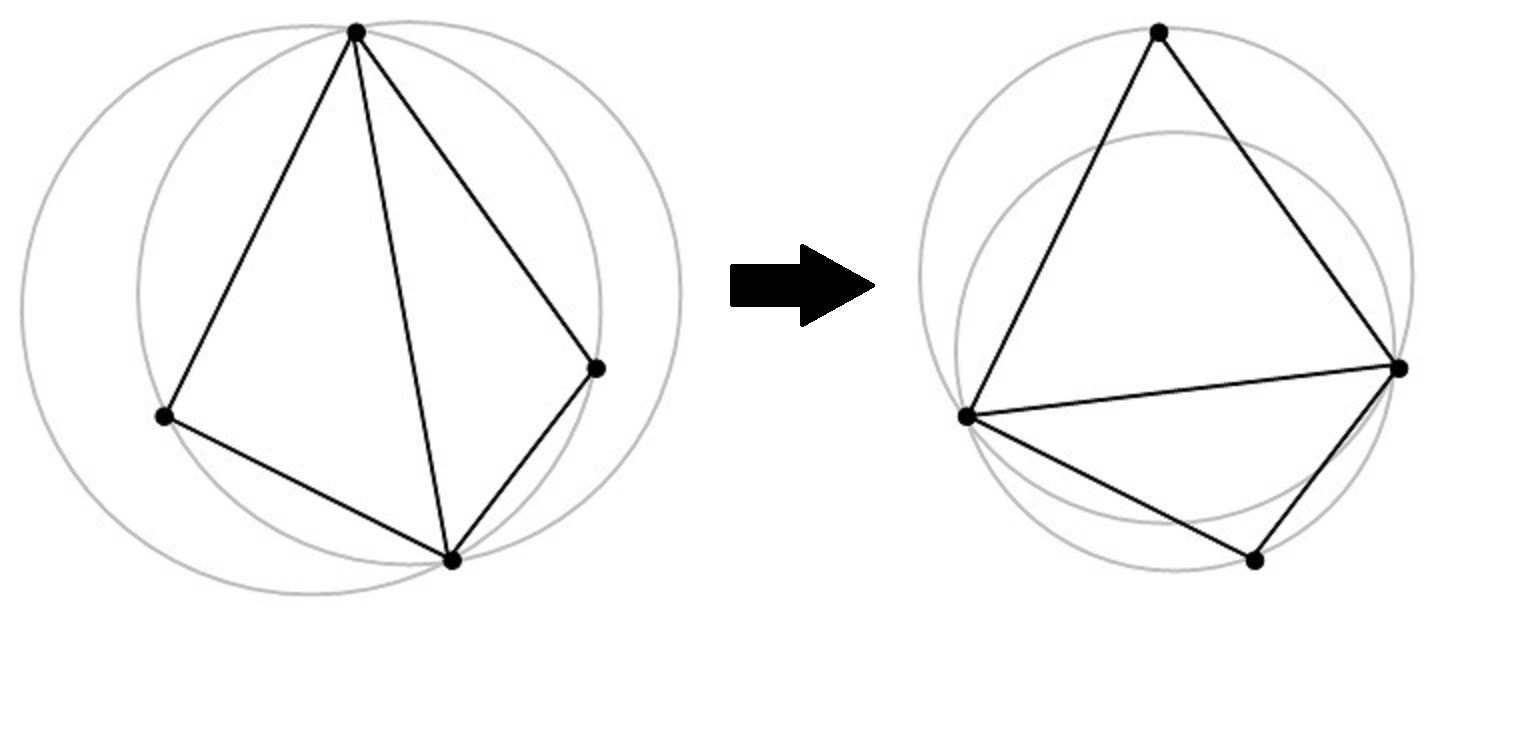
\includegraphics[scale=0.4]{umkreis.jpg}
\caption{Flip einer gemeinsamen Kante, damit Delaunay-Bedingung erfüllt wird}
\end{figure}

Anschließend existieren weitere Dreiecke, die DB potentiell verletzen könnten. Es werden nacheinander alle Dreiecke überprüft und gegebenenfalls Flips durchgeführt, bis die Bedingung global erfüllt ist.
\\

Während der Triangulierung werden Informationen zu Knoten, Kanten und Oberflächen in einer Datenbank für das spätere Clustering gespeichert:

\begin{figure}[H]
\centering
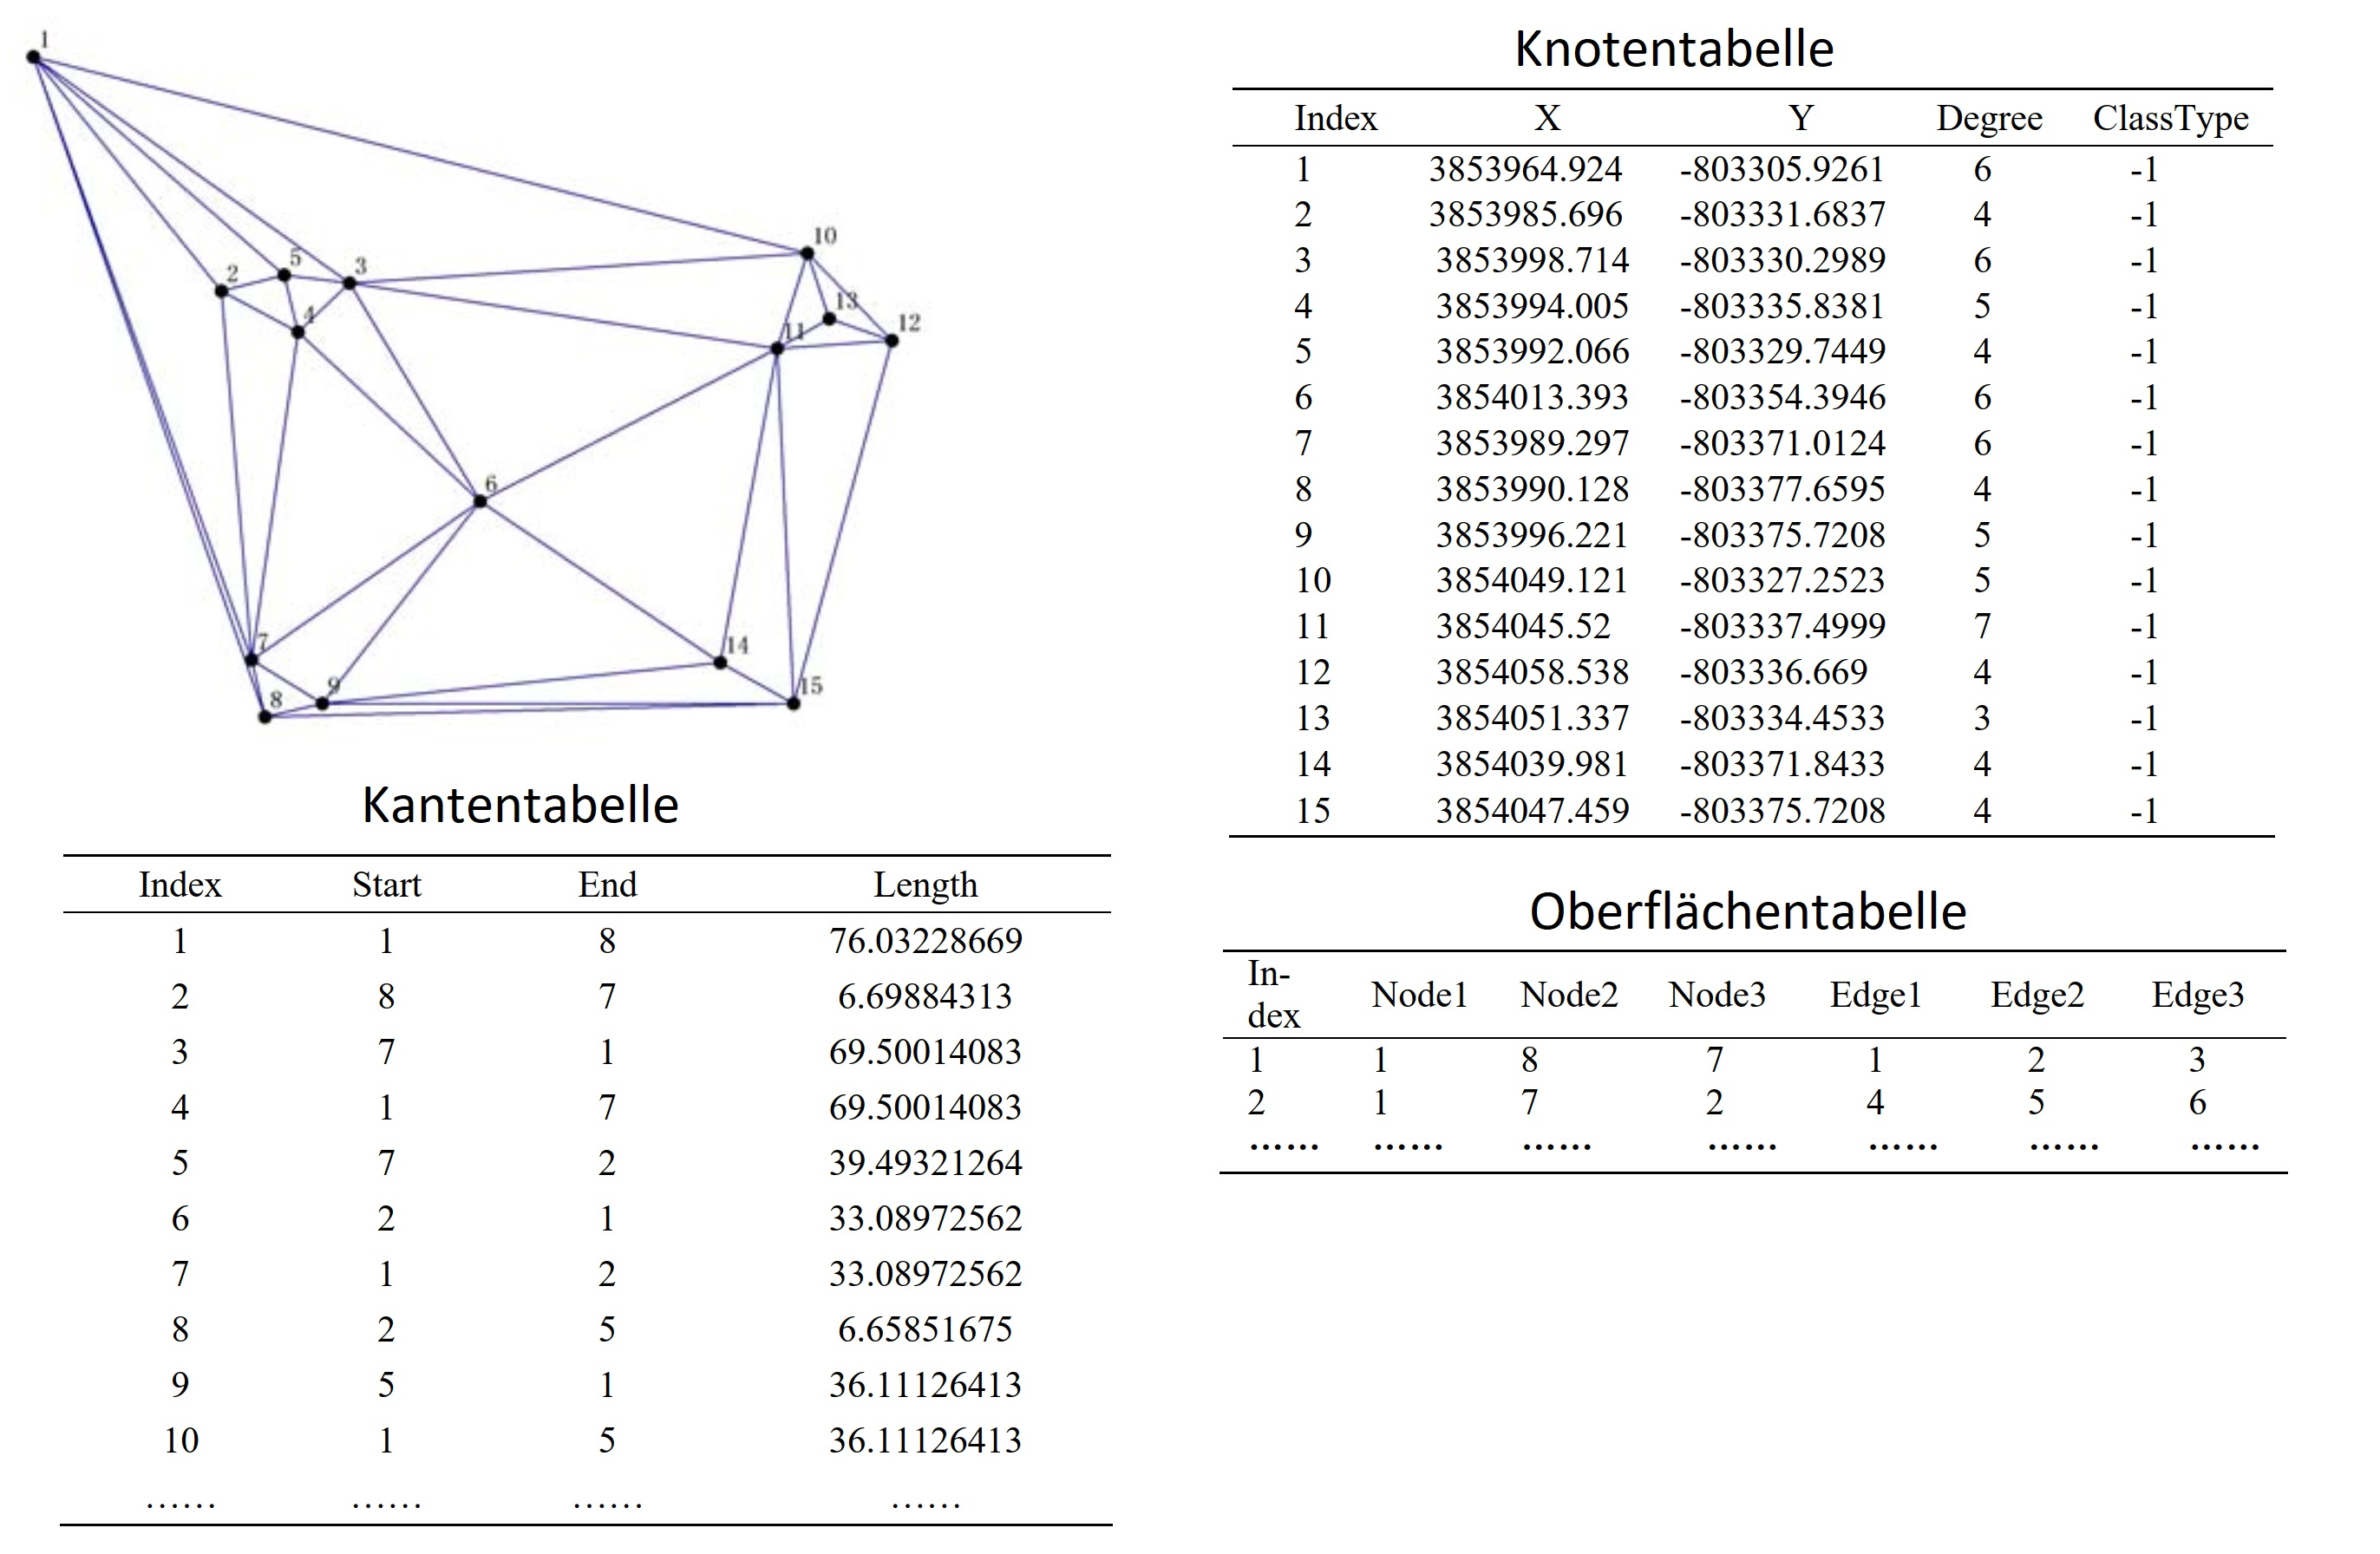
\includegraphics[scale=0.3]{delaunayinfo.jpg}
\caption{Beispiel einer DT von 15 Datenpunkten mit Tabellen für sämtliche Informationen}
\end{figure}

Die Knotentabelle enthält zu jedem der $15$ Punkte die Koordinaten, den Knotengrad und die Kategorie bzw. die Clusternummer ($-1 = Outlier$).\\
Die Kantentabelle enthält Infos zur Richtung der Kanten, wobei $Start=1$ und $End=8$ bedeutet, dass von Knoten $1$ eine gerichtete Kante in Richtung des Knoten $8$ zeigt. Außerdem besitzt sie die Länge $76$.
\\
Die Oberflächentabelle enthält alle Knoten und Kanten, die an den jeweiligen Ebenen (Dreiecken) beteiligt sind.

Im Gegensatz zur gewöhnlichen Delaunay Triangulation sollen in diesem Verfahren nur solche Knoten verbunden werden, welche näher beieinander liegen, als ein vorgegebenes Ähnlichkeitsmaß.
\\

\subsubsection{Bezeichnungen}
Im Folgenden werden Kanten $e_k$ geschrieben als $(p_i,p_j)$, wobei $p_i$ der Startpunkt ist und $p_j$ der Endpunkt. $N(p_i)$ bezeichnet die Menge aller eingehenden und ausgehenden Kanten von Knoten $p_i$. Die lokale Durchschnittslänge $local_mean(p_i)$ ist die durchschnittliche Länge aller Kanten in $N(p_i)$:

$$local\_mean(p_i) =\frac{\sum\limits_{j=1}^{deg(p_i)} len(e_j)}{deg(p_i)}$$

Die globale Durchschnittslänge ist definiert als Durchschnittslänge aller Kanten in $E$.

$$global\_mean(X) =\frac{\sum\limits_{j=1}^{|E|} len(e_j)}{|E|}$$

Die globale Standardabweichung ist die durchschnittliche Abweichung des $global\_mean$ von allen Kantenlängen:

$$global\_sta\_dev(X)= \frac{\sqrt{\sum\limits_{i=0}^n \left(global\_mean(X)-len(e_i)\right)^2}}{n}$$

Der relative Durchschnitt ist das Verhältnis von lokalem zu globalem Durchschnitt:

$$relative\_mean(p_i) = \frac{local\_mean(p_i)}{global\_mean(X)}$$

Eine Kante wird als positive Kante bezeichnet, wenn sie kleiner ist, als das Kriterium $F(p_i)$. Positive Kanten und dazu inzidente Punkte formen einen neuen Wahrscheinlichkeitsgraphen, der gleichzeitig Subgraph der Delaunay-Triangulation ist. Das Kriterium berechnet sich wie folgt:

$$F(p_i) = global\_mean(X) + global\_sta\_dev(X) \times \frac{global\_mean(X)}{local\_mean(p_i)}$$

Ein positiver Pfad ist ein Pfad von positiven Kanten und alle verbundenen Punkte gehören zu einem Cluster.

Die effektive Region des Punktes $p$ mit Radius $\delta$ ist wie folgt definiert:

$$p_{\delta} = \{x|\enspace|x-p|<\delta, p\in X,\forall x\in \mathbb{R}^2\}$$

Die effektive Region einer Punktmenge ist dann die Vereinigung der effektiven Regionen aller Punkte dieser Menge:

$$\overline{X} = \bigcup_{p\in X} p_{\delta}$$

Die $\gamma$-Grenze ist die Menge aller Punkte im Kreis mit Radius $\delta$

$$V_\gamma = \overline{V_{\gamma}} \bigcap V, \qquad \overline{V_{\gamma}} = 
\frac{\overline{V}}
{\{\overline{V} \Theta \gamma Dm(\delta)\}} 
, \enspace \gamma>1$$


mit 

$$Dm = \{x|\enspace |x|\leqslant \delta\}$$

Die $\gamma$-Kurve ist die Mannigfaltigkeit des Punktes in der $\gamma$-Grenze einer Punktemenge.\\

Der Algorithmus für NSCABDT kann wie folgt beschrieben werden:

Zu Beginn gehört kein Punkt einer gegebenen Punktemenge $S$ zu einem Cluster. Außerdem ist die Menge der Punkte des ersten Clusters $C$ leer: $C=\emptyset$
\begin{enumerate}
\item Delaunay-Triangulation berechnen und dabei die Knoten, Kanten und Flächentabellen ausfüllen.
\item Für jeden Punkt $p_i \in S$ alle inzidenten Kanten $N(p_i)$ finden, $local_mean(p_i)$ und $F(p_i)$ berechnen.
\item Für jede Kante $e \in N(p_i)$: Wenn $len(e) \geqslant F(p_i)$, dann Kante aus DT entfernen.
\item Wenn $deg(p_i)=0$, Knoten $p_i$ löschen, ansonsten zu $C$ hinzufügen.
\item Iterativ für alle Knoten durchführen, mit denen $p_i$ verbunden ist.
\item Grenze von Cluster C extrahieren und alle Brücken eliminieren. Dies erfolgt per Hauptkurvenanalyse, welche eine Generalisierung der Hauptachsenanalyse ist. Wenn für einen Cluster zwei verschiedene Grenzen gefunden werden kann, ist dies ein Indiz dafür, dass es zwei kleinere Cluster gibt, die über eine Brücke verbunden sind. Der Algorithmus zur Eliminierung von Brücken lautet wie folgt:
\begin{enumerate}
\item Setze $\delta$ auf die Medianlänge aller Kanten $E$
\item Berechne die effektive Region einer Punktemenge $V$
\item Berechne die $\gamma$-Grenze von $V$
\item Berechne die $\gamma$-Kurve von $V$
\end{enumerate}
\item Gibt es noch unbearbeitete Knoten, obwohl im Iterationsprozess alle Knoten positiver Pfade betrachtet wurden, dann konnten nicht alle Knoten erreicht werden und es mussten zu lange Kanten gelöscht werden (negative Pfade). Es wird ein neuer Cluster $C'$ erstellt und die Iteration mit einem beliebigen unbearbeiteten Punkt fortgesetzt.
\end{enumerate}



\begin{minipage}{0.45\textwidth}\raggedright
\subsubsection{Clusteringergebnisse} ~\\
In der Originalpublikation wird untersucht, wie sich der NSCABDT-Algorithmus beim Clustern von drei verschieden geformten Polygonen verhält. Diese bestehen aus mehreren Hundert Punkten und sind von Outliern umgeben. Außerdem sind zwei Polygone über mehrere Brücken verbunden.
\end{minipage}
\hfill
\begin{minipage}{0.5\textwidth}
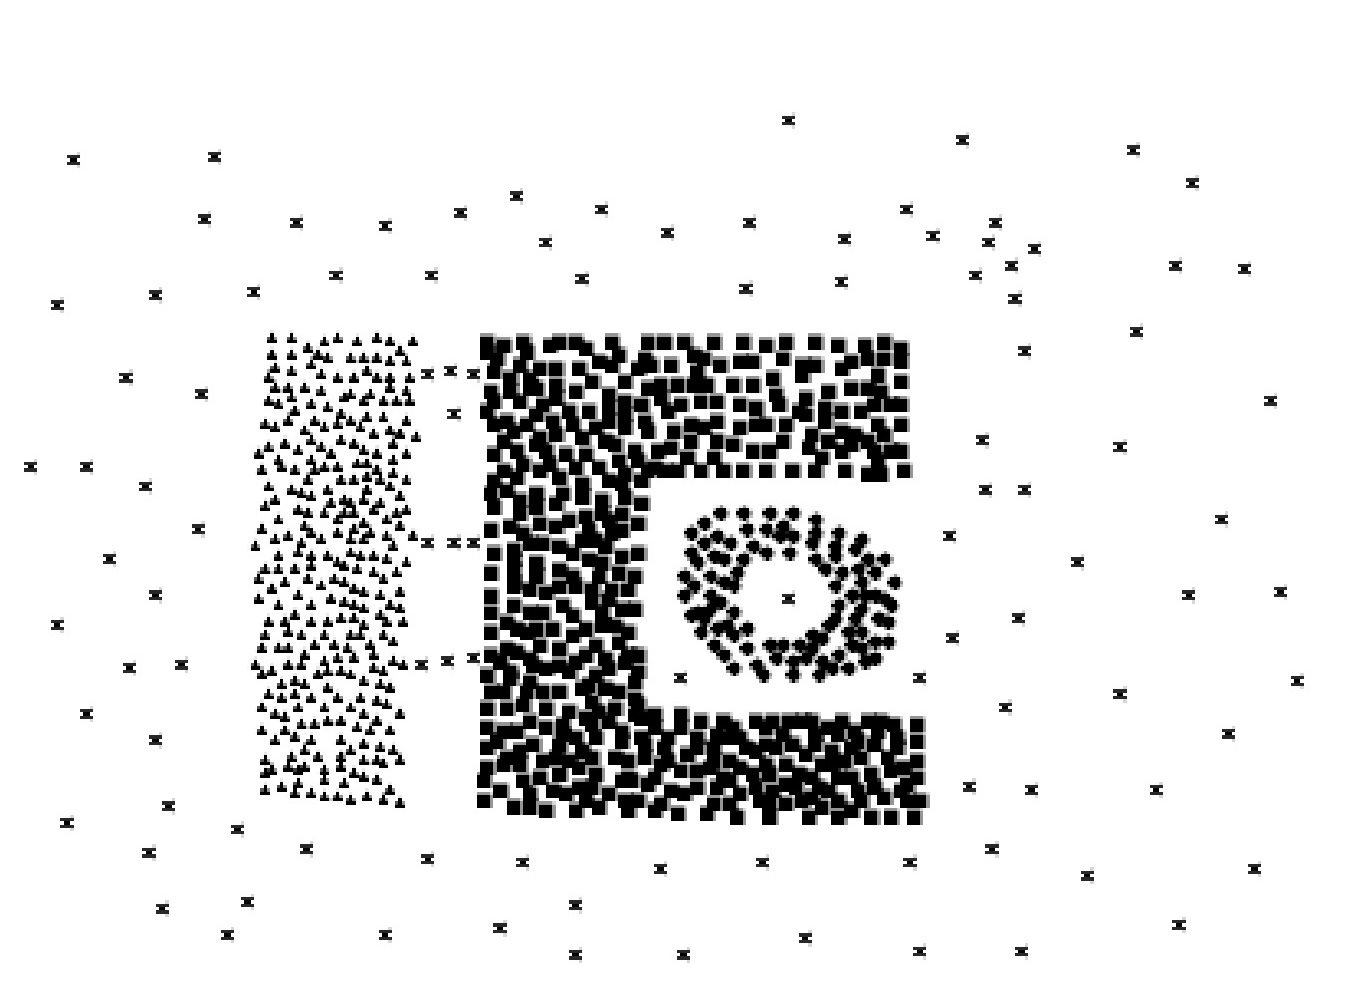
\includegraphics[width=\linewidth]{polygone.jpg}
\captionof{figure}{Beispieldatensatz mit drei Clustern}
\end{minipage}

\vspace{\belowdisplayskip}

Im direkten Vergleich mit DBSCAN ist der NSCABDT-Algorithmus zwar viel langsamer, findet jedoch in jedem untersuchten Fall die korrekten Cluster mit etwas höherer Genauigkeit.
\begin{figure}[H]
\centering
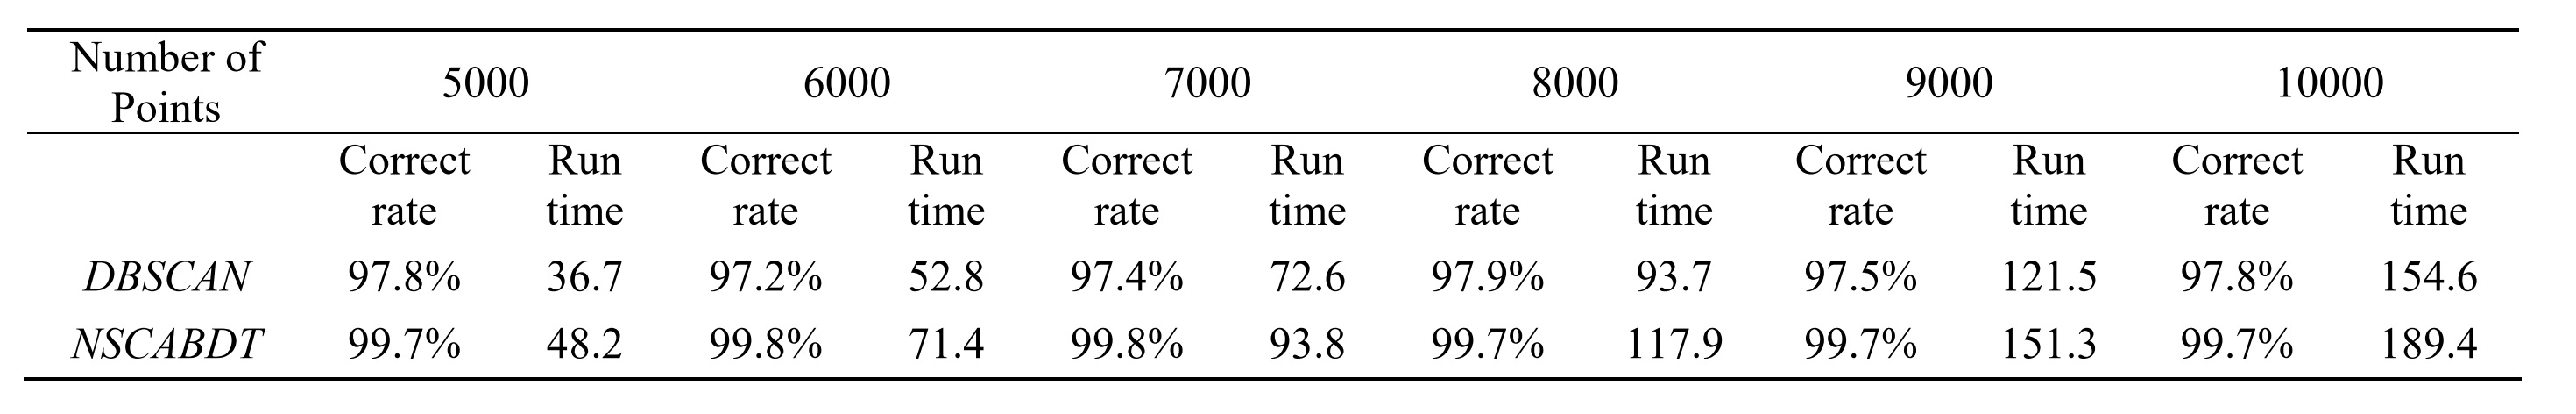
\includegraphics[scale=0.35]{nscabdtaccuracy.jpg}
\caption{NSCABDT schlägt DBSCAN immer, braucht dafür aber länger}
\end{figure}



\pagebreak
\hspace{0pt}
\vfill
\subsection{Graphbasiertes Clustering II (NSFCDT)}

Eine weitere Optimierung, die zwei Jahre später vorgestellt wurde, basiert ebenfalls auf der Delaunay-Triangulation mit anschließendem Fuzzy Refinement. Ein Hauptvorteil gegenüber NSCABDT ist eine deutlich verbesserte Laufzeiteffizienz bei gleichwertigen Ergebnissen \cite{nsfcdt}. Die Methode wurde speziell für Datensätze mit vielen Einträgen entwickelt. Daher eignet sie sich besonders zum Clustern von Rasterbildern.\\~\\

Das Verfahren besteht aus zwei Schritten. Im ersten Schritt wird die Delaunay Triangulation berechnet und ein ähnlichkeitsbasiertes Clustering gebildet. Im zweiten Schritt wird eine Fuzzy-Logik zur Verfeinerung der Ergebnisse angewandt.\\~\\

Der folgende Algorithmus beschreibt den ersten Schritt des Verfahrens. Er nimmt einen Datensatz $X$ mit $n$ Punkten entgegen und clustert ihn auf Basis der Delaunay-Triangulation ($DT$). In der Originalpublikation wird für die Erzeugung der $DT$ der Bowyer-Watson Algorithmus empfohlen, der nur $\mathcal{O}(n\log{}n)$ Operationen benötigt, um $n$ Punkte zu triangulieren und somit besonders effizient ist. Anschließend startet in Zeile $5$ die harte Partitionierung. Dabei wird für ein Initialdreieck aus $DT$ geprüft, ob es größer ist, als ein bestimmter Schwellwert und ob es noch nicht besucht wurde. Wurde ein Initialdreieck gefunden, das klein genug ist, werden von ihm aus alle Nachbarn (Dreiecke, die sich mit dem Initialdreieck eine Kante teilen) betrachtet. Für jedes Nachbardreieck wird geprüft, ob es klein genug ist. Ist dies der Fall, wird es auf einen Stack gelegt. Alle zu großen Nachbardreiecke werden hingegen ignoriert. Der Algorithmus wird solange fortgesetzt, bis alle Elemente auf dem Stack abgearbeitet wurden und kein gültiger Nachbar eines Stackelements mehr gefunden werden konnte. Die Menge der gültigen Nachbardreiecke inklusive Initialdreieck bilden dann einen Cluster. Der Algorithmus wird danach für alle unbesuchten Initialdreiecke aus $DT$ fortgesetzt. Zum Schluss enthält die Menge $ClusterSet$ Mengen von Dreiecken, die die Cluster des Datensatzes bilden.

\vfill
\hspace{0pt}
\pagebreak


\begin{algorithm}[H]
\caption{ Schritt 1: Delaunay Klassifikation}\label{nsfcdt}
\hspace*{\algorithmicindent} \textbf{Input:} $X=\{x_1,\dots,x_n\}$ 
\begin{algorithmic}[1]
\State $DT \gets \textsc{Delaunay}\textsc{Triangles}(X)$
\State $ClusterSet \gets \emptyset$
\State $NewSet \gets \emptyset$
\State $TmpSet \gets \emptyset$
\ForAll{$dt \in DT$}
\If{$\textsc{Visited}(dt) = False$}
\State $\textsc{Initialize}(NewSet)$
\State $\textsc{Push}(dt,Stack)$
\While{$\textsc{Empty}(Stack) = False$}
\State $Triangle\,T \gets \textsc{Pop}(Stack)$
\If{$\textsc{Satisfiable}(T)\,\&\,\textsc{Not}\textsc{Visited}(T)$}
\State $T.Visited \gets True$
\State $NewSet \gets NewSet \cup \{T\}$
\State $TmpSet \gets \textsc{Neighbours}(T)$
\ForAll{$Element \in TmpSet$}
\If{$\textsc{Not}\textsc{Visited}(Element)$}
\State $\textsc{Push}(Element,Stack)$
\EndIf
\EndFor
\EndIf
\EndWhile
\State $ClusterSet \gets ClusterSet \cup newSet$
\EndIf
\EndFor
\end{algorithmic}
\end{algorithm}

Im zweiten Schritt wird eine Fuzzy-Funktion angewandt, um das Clustering zu verfeinern. Dies ist notwendig, um Dichteabfälle an den Randbereichen großer Cluster zu erkennen. Beispielsweise hat ein Wald keine harte Grenze, an der das Baumwachstum plötzlich aufhört. Auch die Bäume in den weniger dichten äußeren Regionen sollten dem Waldcluster zugeordnet werden. Gleichzeitig soll die Größe der Randregionen bei zunehmender Größe des Kernwaldes ebenfalls zunehmen. Die hierzu erforderliche Fuzzy-Zugehörigkeitsfunktion lautet:

$\mu(x:\alpha,\beta) = \left\{
\begin{array}{ll}
0 & x < \alpha \\
2\cdot\left(\frac{x-\alpha}{\beta-\alpha}\right)^2 & \alpha \leqslant x < \frac{\alpha + \beta}{2} \\
1-2\cdot\left(\frac{x-\beta}{\beta-\alpha}\right)^2 & \frac{\alpha + \beta}{2} \leqslant x < \beta \\
1 & x \geqslant \beta
\end{array}
\right. $

Es handelt sich hierbei um eine Sigmoidfunktion. Der Parameter $\alpha$ gibt den Wendepunkt der Kurve an, der Parameter $\beta$ bestimmt die Neigung der Kurve, welche mit zunehmendem $\beta$ immer flacher wird. Je nach Klasseneigenschaft können die Fuzzy-Parameter variiert werden. Beispielsweise könnte die Baumart Buche, die einem Nadelwald steht, eine steilere Zugehörigkeitskurve besitzen, als die Baumart Tanne. Dies bedeutet, dass eine Buche gegenüber einer Tanne viel näher an einem Nadelkernwald stehen muss, um mit einer hohen Zugehörigkeit klassifiziert zu werden. 
\\
Der Funktionswert $\mu$ wird als Stärke der Inklusion bezeichnet. Je größer dieser Wert wird, desto größer wird der Randbereich, in dem weitere Punkte berücksichtigt werden.\\
Der Gesamtalgorithmus inklusive Triangulation und Fuzzy Refinement sieht dann folgendermaßen aus:

\begin{algorithm}[H]
\caption{Fuzzy Basiertes NSFCDT}\label{nsfcdt}
\hspace*{\algorithmicindent} \textbf{Input:} $X=\{x_1,\dots,x_n\}$ 
\begin{algorithmic}[1]
\State $\textsc{Build} (ClusterSet)$
\ForAll{$C_i \in ClusterSet$}
\State $Area \gets \textsc{Get}\textsc{Area}(C_i)$
\State $Degree \gets \textsc{Get}\textsc{Fuzzy}\textsc{Degree}(Area)$
\State $\textsc{Set}\textsc{Satisfiability}\textsc{Condition}(Degree)$
\ForAll{$Triangle \in Cluster$ }
\State $N \gets Neighbour(Triangle)$
\ForAll{$E \in N$}
\If{$\textsc{Fuzzy}\textsc{Satisfiable}(E)$}
\If{$E\in C_j, \forall j\in \{1\dots m\} \,\&\, j\neq i$}
\State $C_i \gets C_i \cup C_j$
\Else 
\State $C_i \gets C_i \cup \{E\}$
\EndIf
\EndIf
\EndFor
\EndFor
\EndFor
\end{algorithmic}
\end{algorithm} 

\subsubsection{Ergebnisse}
Die Untersuchung hat gezeigt, dass NSFCDT gegenüber NSCABDT bei größeren Datensätzen eine bessere Laufzeit besitzt, vor allem, wenn der Refinement-Schritt weggelassen wird. Bei kleineren Datensätzen ist das fuzzy NSFCDT etwas langsamer, erzielt jedoch bessere Ergebnisse, da manche Cluster sinnvollerweise verschmolzen werden können.

\begin{figure}[H]
\centering
\includegraphics[scale=0.33]{nsfcomp.jpg}
\caption{Laufzeiten von NSFCDT und NSCABDT bei verschieden großen Datensätzen}
\end{figure}

So wurde zum Beispiel ein Graustufenbild einer indischen Stadt mit NSFCDT sowohl mit als auch ohne Refinement geclustert. Die Fuzzy-Methode fand dabei vier Gebiete mit Baumbestand. Die harte Methode jedoch unterteilte zwei der Gebiete in zwei weitere Cluster, obwohl dies zu fragwürdigen Ergebnissen führte. Die Untersuchung zeigt, welch hohes Potential das fuzzy-basierte NSFCDT beim Clustern von großen Datensätzen mit variablen Eigenschaften besitzt. So führt die Unterscheidung zwischen Gebäuden, Flüssen und Wäldern bei der Berechnung des Inklusionsfaktors  (jeweils individuelle Fuzzy-Kurve) dazu, dass für jede Klasse sehr präzise Clusteringergebnisse gefunden werden können, welche die Präzision des NSCABDT-Algorithmus deutlich übertreffen.

\begin{figure}[H]
\centering
\includegraphics[scale=0.4]{nsfcdtres.jpg}
\caption{Clusteringergebnis nach hartem NSFCDT (links) und nach dem Fuzzy Refinement (rechts)}
\end{figure}


Als Vorteil sehen die Autoren, dass die Gesamtlaufzeit des Algorithmus mit $\mathcal{O}n\sqrt{n}$ sehr klein ist. Trotzdem fügen Sie hinzu, dass es noch viel Spielraum für Verbesserungen gibt. So können zwei benachbarte Dreiecke nicht berücksichtigt werden, wenn sie anstelle einer gemeinsamen Kante einen gemeinsamen Knoten haben. Dieses Problem kann nur durch einen weiteren Teilalgorithmus gelöst werden. Außerdem könnten noch effizientere Datenstrukturen oder statistische Modelle zu einer weiteren Verbesserung der Laufzeit führen.
~\\

Eine vollständige Implementierung und Demonstration des Algorithmus anhand zweier Beispiele ist im Anhang ab Zeile 15 zu finden.
 
\clearpage

\subsection{Kontextbasiertes geographisch gewichtetes Fuzzy-Clustering (CFGWC)}
Eine weiteres FCM-basiertes Clusteringverfahren wurde im Hinblick auf die geodemografische Analyse entwickelt, das CFGWC \cite{cfgwc}. Die Geodemografie ist die Wissenschaft von der Entstehung von menschlichen Populationszentren (i.d.R. Städte). Sie verbindet die Demografie, also die Wissenschaft von menschlichen Populationsströmen, mit der Geografie, der Wissenschaft von der physischen Gestalt der Erdoberfläche, dessen Variation und Veränderung. Fuzzy-basierte Clusteringalgorithmen kommen in der Geodemografie häufig zum Einsatz, da Sie das Problem des ökologischen Fehlschlusses vermeiden. Ein ökologischer (oder kollektiver) Fehlschluss ist ein unzulässiger Vergleich von Durchschnittswerten.
Ein Beispiel dafür ist die Reichtumsverteilung in einem Dorf und einer Großstadt. Zwar ist der durchschnittliche Stadtbewohner reicher als der durchschnittliche Dorfbewohner, jedoch kann es trotzdem sein, dass der ärmste Dorfbewohner reicher ist, als der ärmste Stadtbewohner, da Städte eine anziehende Wirkung auf arme Menschen haben. Gleichzeitig ist es durch eine stark komprimierte Reichtumsanhäufung einer Elite auch möglich, dass es mehr arme Stadtbewohner als arme Dorfbewohner gibt.
Obwohl der FCM-Algorithmus dieses Problem im Gegensatz zu harten Clusteringalgorithmen verhindert, fehlt ihm eine geografische Komponente. Zum Beispiel können zwei Wohngebiete mit gleichen Populationsdaten, aber unterschiedlicher Lage vollkommen unterschiedlich interpretiert werden. Aus diesem Grund wurde eine Modifikation für die Berechnung der Zugehörigkeitsmatrix in FCM entwickelt, die den sogenannten Nachbarschaftseffekt berücksichtigt. Als Nachbarschaftseffekt bezeichnet man die Art der Beeinflussung des Verhaltens eines Menschen in Abhängigkeit von seiner Wohnlage und Nachbarschaft:

$$u_{jk}^{\prime} = \alpha \times u_{jk}+\beta \times \frac{1}{A} \times \sum\limits_{i=1}^c \omega_{ji} \times u _{ik}$$

Dieser dritte Schritt erfolgt unmittelbar nach der Aktualisierung von Zugehörigkeitsmatrix und Clusterzentroiden noch in der Repeat-Schleife des oben beschriebenen FCM-Algorithmus. Dabei ist $u_{jk}$ die alte Zugehörigkeitsmatrix aus dem vorherigen Schritt und $u_{jk}^{\prime}$ die geografisch gewichtete neue Zugehörigkeitsmatrix. Die Parameter $\alpha$ und $\beta$ legen fest, wie stark die alten Zugehörigkeiten in die Berechnung einfließen sollen, wobei $\alpha + \beta = 1$. Parameter $A$ sorgt dafür, dass die Summe der Zugehörigkeiten eines Punktes zu einem Gebiet für alle Gebiete stets dem Kontextgrad $f_k$ (wird später erklärt) entspricht. Die gewichtete Zugehörigkeit wird folgendermaßen berechnet:

$$\omega_{ji} = \frac{\left(m_j \times m_i\right)^b}{d_{ji}^{a}}$$

Dabei stehen $m_i$ und $m_j$ für die Einwohnerzahlen der Gebiete $i$ bzw. $j$ und $d_{ji}^a$ ist die Distanz zwischen beiden Gebieten. Die Parameter $a$ und $b$ können beliebig gewählt werden. 
\\
Weil immer nur eine Teilmenge des Datensatzes eine Bedeutung für den betrachteten Kontext hat, kann die Geschwindigkeit des Algorithmus deutlich beschleunigt werden. Möchte man zum Beispiel nach einem Einkaufszentrum suchen, wird dem Algorithmus die Kontextvariable $shopping$ hinzugefügt, so dass der Suchraum deutlich verkleinert wird.
\\
Sei $y\in X$ die Kontextvariable $y$ aus Datensatz $X$, welche definiert ist als:

\begin{align*}
A \colon &Y \to \left[0,1\right] \\
  &y_k \mapsto f_k = A(y_k).
\end{align*}

Der Wert $f_k$ repräsentiert den Grad der Relation des $k$-ten Punktes zu Kontext $Y$.
\\
Es gilt außerdem:

$$\sum\limits_{j=1}^c u_{jk} = f_k,\, \forall k\in\{1,\dots,n\}$$
und 
$$\sum\limits_{k=1}^n u_{jk} < n, \, \forall j \in \{1,\dots ,c \}$$
Die Aktualisierung der Clusterzentroide entspricht der Methode im originalen FCM-Algorithmus. Die Zugehörigkeitsmatrix wird hingegen wie folgt berechnet:

$$u_{jk}=\frac{f_k}{\sum\limits_{i=1}^c \left(\frac{||x_k-v_j||}{||x_k-v_i||}\right)^{\frac{2}{m-1}}},\, \forall k\in\{1,\dots,n\},\,\forall j\in\{1,\dots,c\}$$

Die alternierende Optimierung bricht ab, wenn die aus einem Schleifendurchlauf resultierende Zugehörigkeitsmatrix von der Matrix aus dem vorherigen Durchlauf um weniger als $\delta$ abweicht.
\\

Untersuchungen haben gezeigt, dass CFGWC \cite{cfgwc} gegenüber den älteren und konzeptionell unterlegenen Methoden NE \cite{ne} und FGWC \cite{fgwc} performanter ist und zum Zweck der Demografieanalyse die besten Ergebnisse liefert. Für die Zukunft wünschen sich die Autoren weitere Leistungsverbesserungen durch parallele Varianten des Algorithmus.

\section{Bestimmung der optimalen Clusteranzahl}
Clustering wird im Allgemeinen als unüberwachte Lernmethode zur Gruppierung von ähnlichen Daten verstanden. Aus diesem Grund braucht es vor der eigentlichen Partitionierung Methoden, die die optimale Clusteranzahl bestimmen und die Kostenfunktion des betrachteten Partitionierungsprozesses global minimieren.
\\
Eine Methode wurde oben bereits vorgestellt: Der Xie-Beni-Index. Solche Indizes werden im Allgemeinen auch Clustervaliditätsindex genannt. Sie bewerten, wie gut eine Partitionierung für unterschiedliche Clusteranzahlen ist.
\\
Im Folgenden werden weitere Methoden vorgestellt, die aus verschiedenen Clusteringverfahren abgeleitet wurden und nicht somit nicht immer anwendbar sind!

\subsection{Basisalgorithmus}
Das Grundsätzliche Programm zur Berechnung der optimalen Clusteranzahl $c_opt$ ist für jeden CVI identisch und kann wie folgt beschrieben werden:

\begin{algorithm}[H]
\caption{cOpt(X,pFCA,CVI,$c_{max}$)}\label{cvibase}
\begin{algorithmic}[1]
\Require $X$ ist dein d-dimensionaler Datensatz mit $n$ Datenpunkten, $2\leqslant c_{max} \leqslant n$ ist die maximale Clusteranzahl, pFCA ist ein probabilistischer Clusteringalgorithmus, CVI ist ein globales Gütemaß
\State Initialisiere $cvi_{opt}$ mit einem sehr schlechten Wert in Bezug auf das gewählte CVI-Verfahren.
\State $c=1$, $c_{opt} = 1$
\Repeat
\State $c=c+1$
\State Führe Partitionierung $pFCA(X,c)$ durch
\If{$CVI(f)$ der neuen Partitionierung $f$ besser als $CVI_{opt}$}\State $CVI_{opt} = CVI(f)$, $c_{opt} = c$
\EndIf
\Until{$c==c_{max}$}
\State \Return $c_{opt}$, $CVI_{opt}$
\end{algorithmic}
\end{algorithm} 

Zu Beginn wird die optimale Clusteranzahl mit dem Wert $1$ initialisiert. In einer Schleife wird dann für jede mögliche Clusteranzahl zwischen $1$ und $c_{max}$ ermittelt, ob sich das Gütemaß $CVI$ verbessert hat. Es bleiben die optimale Clusteranzahl $c_{opt}$ mit dem zugehörigen CVI-Wert $CVI_{opt}$ hängen.  

\subsection{Normalized Partition Coefficient (NPC)}
Dieses Verfahren \cite{npc} basiert ausschließlich auf der Zugehörigkeitsmatrix. Eine Partitionierung gilt als optimal, wenn Datenpunkte den Clustern klar zugeordnet wurden, die Zugehörigkeitsgrade also nicht zu stark von den Werten $0$ und $1$ abweichen. Implizit wird so die Kompaktheit innerhalb der Cluster bewertet. Der Index berechnet sich wie folgt:
$$V_{PC}(U,c) = \frac{1}{n} \sum\limits_{i=1}^c \sum\limits_{k=1}^n u_{ik}^2$$
Da das Ergebnis aber von der Clusteranzahl $c$ abhängig ist und große Clusteranzahlen automatisch schlechter bewertet werden, wird das Ergebnis zusätzlich normalisiert:

$$V_{NPC}(U,c) = 1- \frac{c}{c-1}\left(1-V_{PC}\right)$$

$V_{NPC}$ nimmt Werte zwischen $0$ und $1$ an, wobei ein möglichst großer Wert auf eine gute Zerlegung hindeutet.
\\~\\
Die Implementierung ist im Anhang in Zeile 37 zu finden, eine Demonstration in den Zeilen 39 und 40.

\subsection{Kim-Kim-Lee-Lee Index (KKLL)}
Eine andere Variante, die ebenfalls nur auf den relativen Zugehörigkeiten der Daten beruht, ist der Kim-Kim-Lee-Lee Index \cite{kkll}. Er berechnet die durchschnittliche Überlappung zwischen den Clusterpaaren als relativen Grad der Teilung der Datenpunkte in der Überlappung. Die Partitionierung ist optimal, wenn der Überlappungsgrad am Kleinsten ist.

Der relative Grad der Teilung eines Datenpunktes $x_k$ zwischen zwei
Clustern $C_i$ und $C_j$ ist wie folgt definiert:

$$S_{rel}(x_k\colon C_i,C_j) = \frac{u_{ik} \land u_{jk}}{\frac{1}{c} \sum\limits_{l=1}^c u_{lk}}$$

Der binäre Fuzzy-AND-Operator ist definiert als Minimum der beiden Parameter: $min(u_{ik}, u_{jk})$.

Der relative Grad der Teilung zwischen zwei Clustern $C_i$ und $C_j$ definiert sich folgendermaßen:

$$S_{rel}(C_i,C_j) = \sum_{k=1}^n c\cdot \left[u_{ik} \land u_{jk}\right] h(x_k) \text{ mit } h(x_k) = -\sum_{i=1}^c u_{ik}\cdot log_a(u_{ik})$$

Dabei soll die Entropie $h(x_k)$ der Datenpunkte deren Vagheit verstärken. Als Entropie kann man den Grad der Abweichung von einer Gleichverteilung verstehen. Je ungleichmäßiger also die Verteilung der Daten ist, desto kleiner wird der relative Clusterteilungsgrad.
\\
Der Kim-Kim-Lee-Lee Index ist dann definiert als durchschnittlicher
relativer Grad der Teilung zwischen allen möglichen Clusterpaaren:

$$V_{KKLL}(U) = \frac{2}{c(c-1)} \sum_{i=1}^{c-1} \sum_{j=i+1}^c \sum_{k=1}^n \left[c \cdot \left[u_{ik} \land u_{jk} \right]\cdot h(x_k)\right]$$

Die Zerlegung ist optimal, wenn $V_{KKLL}$ einen möglichst kleinen Wert annimmt.

\subsection{Fuzzy Hypervolume/Partition Density (FHV/PD)}
Die CVI-Methode Fuzzy Hypervolume \cite{fhv} bewertet nicht nur die relativen Entfernungen der Datenpunkte zu ihren Clustern, sondern insgesamt die Kompaktheit der gesamten Zerlegung. FHV bewertet eine Partitionierung als gut, wenn die Summe der Clustervolumina möglichst klein ist. Dabei lässt sich das Volumen eines Clusters über die Determinante der Datenerzeugenden Kovarianzmatrix berechnen: 

$$Cov_i = \frac{\sum\limits_{k=1}^n (u_{ik})^m (x_k-v_i)(x_k-v_i)^{\top}}{\sum\limits_{k=1}^n (u_{ik})^m} \text{,\ für \quad} 1\leqslant i\leqslant c$$

und

$$V_{FHV}(U,X,V) = \sum_{i=1}^c \sqrt{\det(Cov_i)}$$

Da eine Kovarianzmatrix sowohl die Ausdehnung und Richtung einer Punktwolke beschreibt, kann Fuzzy Hypervolume entsprechend unterschiedlich große und geformte Cluster erkennen. Dies ist gegenüber anderen Verfahren ein erheblicher Vorteil. Ein Nachteil ist, dass die optimale Clusteranzahl für $c=n$ erreicht wird. Aus diesem Grund muss manuell überprüft werden, ab wann die Erhöhung der Clusteranzahl nicht mehr wesentlich zu einer Verbesserung der Partitionierungsergebnisse beiträgt. Außerdem werden große Cluster mit vielen Punkten automatisch schlechter bewertet. Aus diesem Grund wurde eine Verbesserung vorgeschlagen, die Partition Density (PC):

$$V_{PD}=\frac{\sum\limits_{i=1}^c \sum\limits_{k=1}^n u_{ik}}{V_{FHV}},\quad \forall x_k \in \{x_k|(x_k-v_i)^{\top}\cdot Cov_i^{-1}\cdot(x_k-v_i)<1\}$$

Diese basiert auf dem physikalischen Prinzip \textit{Dichte ist Masse pro Volumen} ($\rho = \frac{m}{V}$). Die Zerlegung ist optimal, wenn die Cluster möglichst dicht sind, also $V_{PD}$ einen großen Wert hat. Partition Density erhält alle Eigenschaften von Fuzzy Hypervolume, verringert aber die Präferenz für kleine Cluster. Da die monoton fallende Tendenz für $c \rightarrow n$ noch verschärft wird, muss auch hier manuell evaluiert werden, ab wann eine weitere Inkrementierung der Clusteranzahl nicht mehr sinnvoll ist.
\\~\\
Die Implementierung ist im Anhang in Zeile 38 zu finden, eine Demonstration in den Zeilen 39 und 40.

\subsection{Zahid-Limouri-Essaid Index (ZLE)}
Eine weitere Klasse von Clustervaliditätsindizes basiert auf der gleichzeitigen Optimierung von Kompaktheit und Separation \cite{zle}:
\begin{itemize}
\item \textbf{Kompaktheit} Datenpunkte innerhalb eines Clusters sind möglichst ähnlich zueinander
\item \textbf{Separation} Datenpunkte aus unterschiedlichen Clustern sind möglichst verschieden
\end{itemize}

Ein bereits vorgestelltes Verfahren aus dieser Klasse von CVI ist der Xie-Beni-Index. Der Zahid-Limouri-Essaid Index kombiniert die Ideen aus dem Xie-Beni Index, dem Kim-Kim-Lee-Lee Index und einem weiteren Verfahren - dem Fukuyama-Sugeno Index. \\

Funktion $SC_1$ berechnet die geometrische Struktur als das Verhältnis von der Streuung der Clusterprototypen (Fukuyama-Sugeno Index) zur Kompaktheit innerhalb der Cluster (Summe der quadrierten Abstände zwischen Clusterzentroiden und Datenpunkten - Xie-Beni Index):

$$SC_1(X,U,V) = \frac{\frac{\sum\limits_{i=1}^c ||v_i-\overline{x}||_A^2}{c}}{\sum\limits_{i=1}^c\left(\frac{\sum\limits_{k=1}^n u_{ik}^2 \cdot ||x_k-v_i||^2}{\sum\limits_{k=1}^n u_{ik}}\right)}$$

Die Funktion $SC_2$ ermittelt die Partitionierungsstruktur wieder als das Verhältnis von Separations- zu Kompaktheitsmaßen. Die Separation ist hierbei durch die Überlappung zwischen den Clusterpaaren gegeben (Kim-Kim-Lee-Lee Index). Das Kompaktheitsmaß ist die Summe aller Kompaktheitsmaße aller Datenpunkte, wobei das Kompaktheitsmaß eines Datenpunktes als größter Zugehörigkeitsgrad unter den Clustern definiert ist: 

$$SC_2(U) = \frac{\sum\limits_{i=1}^{c-1} \sum\limits_{j=i+1}^c\frac{\sum\limits_{k=1}^n \min(u_{ik},u_{jk})^2}{\sum\limits_{k=1}^n \min(u_{ik},u_{jk})}}{\frac{\sum\limits_{k=1}^n \max_{1\leqslant i \leqslant c}(u_{ik})^2}{\sum\limits_{k=1}^n \max_{1\leqslant i \leqslant c}u_{ik}}}$$ 

ZLE kombiniert beide Funktionen, wobei $SC_1$ maximiert und $SC_2$ minimiert wird.
$$V_{ZLE}(U,V,X) = SC_1(U,V,X)-SC_2(U)$$
Die optimale Clusteranzahl wird durch Maximierung von
$V_{ZLE}$ über dem Intervall $\left[c_{min},\dots,c_{max}\right]$ berechnet.


\subsection{Visual Assessment for Cluster Tendency (VAT)}
\begin{minipage}{0.35\textwidth}\raggedright
Neben der automatischen Bestimmung der optimalen Clusteranzahl gibt es auch diverse semiautomatische Verfahren, die es dem Benutzer möglich machen, die korrekte Clusteranzahl einfach abzulesen. Der VAT-Algorithmus erreicht dies, indem er die paarweisen Unähnlichkeiten zwischen den Daten als Graustufenbild visualisiert und so umsortiert, dass die Cluster entlang der Hauptdiagonalen als dunkle Blöcke zu erkennen sind.
\end{minipage}
\hfill
\begin{minipage}{0.6\textwidth}
\includegraphics[width=\linewidth]{vatalg.jpg}
\captionof{figure}{Paarweise Unähnlichkeiten zwischen Datenpunkten als Matrix und Graustufenbild vor und nach Anwendung des VAT-Algorithmus}
\end{minipage}
 
\vspace{\belowdisplayskip}

Der Sortierprozess kann wie folgt beschrieben werden:
\begin{algorithm}[H]
\caption{$VAT(R)$}\label{vatalg}
\begin{algorithmic}[1]
\Require{$R = \left[r_{ij}\right]$ ist eine $n \times n$ Matrix von paarweisen Unähnlichkeiten mit $r_{ii} = 0$ und $r_{ij} \geqslant 0, \, \forall i,j \in \{1,\dots,n\}$}
\State Initialisiere $I=\emptyset$; $J=\{1,2,\dots,n\}$; $P = (0,0,\dots,0)$
\State Bestimme $(i,j)\in \argmax\limits_{p\in J, q\in J}\{r_{pq}\}$
\State Setze $P(1)=j$; ersetze $I = I \cup \{j\}$ und $J = J - \{j\}$
\For{$t\in \{2,\dots,n\}$}
\State Bestimme $(i,j) \in \argmin\limits_{p\in I, q\in J}\{r_{pq}\}$
\State Setze $P(t) = j$; ersetze $I = I \cup \{j\}$ und $J = J - \{j\}$
\EndFor
\State Berechne $\tilde{R}_{ij} = \left[\tilde{r}_{ij}\right] = \left[r_{P(i)P(j)}\right],\, \forall i,j \in \{1,\dots,n\}$
\State \Return Graustufenbild $I(\tilde{R})$ mit größten Ähnlichkeiten entlang der Hauptdiagonalen
\end{algorithmic}
\end{algorithm}

Die Matrix $r_{ij}$ enthält die Unähnlichkeiten der Punkte $x_i$ und $x_j$ als auf das Intervall $\left[0,1\right]$ normalisiertes Abstandsmaß. Zu Beginn werden die Indizes des größten Unähnlichkeitswertes gesucht, wobei alle Zeilen und Spalten erlaubt sind. Anschließend wird der erste Eintrag des Permutationsvektors $P$ auf den Spaltenindex des gefundenen Eintrags gesetzt. Der Menge der noch zu bearbeitenden Indizes $J$ wird $j$ entzogen, während die Menge der schon bearbeiteten Indizes $I$ $j$ hinzugefügt wird. In einer Schleife wird dieser Vorgang für alle Permutationseinträge von $2$ bis $n$ wiederholt. Im Unterschied zur Initialisierung wird jedoch immer nach den Indizes der kleinsten Unähnlichkeit gesucht und es sind nur solche Spalten und Zeilen erlaubt, die durch Mengen $I$ (erlaubte Zeilen) und $J$ (erlaubte Spalten) gekennzeichnet werden. Die Vertauschung der Matrixwerte mit den Einträgen des Permutationsvektors an den Indizes dieser Werte ergibt schließlich die umsortierte Ergebnismatrix. Diese kann als Graustufenbild visualisiert werden, sodass Ähnlichkeiten möglichst dunkel und Unähnlichkeiten möglichst hell dargestellt werden. Die Anzahl der Quadrate entlang der Hauptdiagonalen entspricht der Clusteranzahl des Datensatzes.
\\
Die Erkennung der Clusteranzahl möchte man unter Umständen keinem Menschen überlassen, da Datensätze sehr groß werden können und Menschen zu unterschiedlichen Ergebnissen kommen. Eine Lösung bietet die automatische Cluster Count Extraction (CCE) \cite{cce}.
\\~\\
Eine Implementierung und Anwendung des VAT-Algorithmus ist im Anhang ab Zeile 41 zu finden.

\section{Vergleich von Clusteringergebnissen}
Partitionierende Clusteringverfahren liefern bei zufälligen Initialisierungen oft sehr unterschiedliche Clusteringergebnisse auf dem gleichen Datensatz. Da sich stark schwankende Ergebnisse schlecht zum Vergleich mit anderen Clusteringverfahren eignen, will man immer nur jeweils die beste Partitionierung finden und mit der besten Partitionierung des anderen Verfahrens vergleichen. Eine weitere Herausforderung stellt der Vergleich der Ausreißersensitivität dar. Während ein Ausreißer beim einen Verfahren kaum eine Auswirkung auf das Endergebnis hat, führt er bei dem anderen Algorithmus zu einer starken Verschlechterung der Ergebnisse. Die folgenden Methoden sollen solche Probleme erkennen. 


\subsection{Rand-Index}
Eine der ersten Methoden zum Vergleichen von harten Partitionierungen wurde bereits 1971 von William M. Rand \cite{rand} vorgestellt. Diese misst die Ähnlichkeit zweier Zerlegungen anhand der Anzahl der Datenpunkte, die in den Clustern beider Zerlegungen gemeinsam vorkommen. \\~\\
Seien $P = \{P_1, \dots, P_k\} \subset 2^X$ und  $Q = \{P_1, \dots, P_l\} \subset 2^X$ zwei harte Partitionierungen von Datensatz $X=\{x_1,\dots,x_n\}$ mit $n$ Datenpunkten. Sowohl in $P$ als auch in $Q$ überschneiden sich zwei verschiedene Cluster nie. Außerdem gibt es keine leeren Cluster und die Vereinigung aller Cluster ergibt den Datensatz. Es sind also alle Datenpunkte einem Cluster zugeordnet. Zwei Elemente $x$ und $x'$ bilden ein gepaartes Elementtupel in $P$, wenn sie zum gleichen Cluster gehören. Es gilt also: $\exists i \in \left[1,\dots,k\right] \text{ mit } x \in P_i \text{ und } x' \in P_i$. Man unterscheidet zwischen vier verschiedenen Paarungsarten:

\begin{itemize}
\item $C_1 \equiv \{(x,x')|  x \text{ und } x' \text{ sind sowohl in } P \text{ als auch in } Q \text{ gepaart}\}$
\item $C_2 \equiv \{(x,x')|  x \text{ und } x' \text{ sind in } P \text{ gepaart, aber nicht in } Q\}$
\item $C_3 \equiv \{(x,x')| x \text{ und } x' \text{ sind in } Q \text{ gepaart, aber nicht in } P\}$
\item $C_4 \equiv \{(x,x')|  x \text{ und } x' \text{ sind weder in } P \text{ noch in } Q \text{ gepaart}\}$
\end{itemize}

Die Tupel aus $C_1 \cup C_4$ heißen konkordante Paare, wohingegen die Tupel aus $C_2 \cup C_3$ diskonkordante Paare genannt werden. Der Rand-Index ist dann definiert als der Anteil der konkordanten Paare an der Menge aller Paare:

$$R(P,Q) = \frac{|C_1|+|C_4|}{|C_1|+|C_2|+|C_3|+|C_4|}, \text{ wobei } R(P,Q) \in \left[0,1 \right]$$

Die zugehörige Distanzfunktion zum Berechnen des Abstands zwischen den beiden Partitionen ist dann einfach $D_R(P,Q) = 1-R(P,Q)$.
\\~\\
Für den Vergleich zweier Fuzzy-Zerlegungen eignet sich dagegen die Variante \textit{Campello's Fuzzy Rand Index}.

\subsection{Subset Similarity Index}
Eine weitere Methode, die eine besonders gute Laufzeit besitzt und somit auf großen Datensätzen zum Einsatz kommt, ist der Subset Similarity Index \cite{subsim}. Dieser basiert auf dem Vergleich von Fuzzy-Clustern aus Partitionierungen $U_{k\times x}$ und $\tilde{U}_{l\times n}$ des Datensatzes $X=\{x_1,\dots,x_n\}$. Angewandt werden kann die Methode sowohl auf harte als auch auf weiche Paritionierungen. Die Ähnlichkeit zwischen zwei Crisp-Clustern ist definiert als Anteil des Schnittes zweier Cluster an ihrer Vereinigung:

$$s_{ij} = \frac{||C_i \cap \tilde{C}_j||}{||C_i \cup \tilde{C}_j||},  \, \forall i \in \left[1,k\right]\text{ und } j \in \left[1,l\right] $$

Die Ähnlichkeit zwischen zwei Fuzzy-Clustern dagegen ist definiert als der Anteil der T-Normen aller Punktepaare beider Cluster an den T-Conormen dieser Punktepaare:

$$s_{ij} = \frac{\sum\limits_{r=1}^n \top(u_{ir},\tilde{u}_{jr})}{\sum\limits_{r=1}^n \bot (u_{ir},\tilde{u}_{jr})},\, \forall i \in \left[1,k\right]\text{ und } j \in \left[1,l\right]$$

Für $\top$ wird in der Regel die Minimumsfunktion und für $\bot$ die Maximumsfunktion eingesetzt (Standardnorm). Weitere Normen sind z.B. die algebraische Norm, Lukasiewicz-Norm, Hamacher-Norm und die Dombi-Norm:

\begin{figure}[H]
\centering
\includegraphics[scale=0.3]{tnorms.jpg}
\caption{Verschiedene T-Normen und T-Conormen auf Zugehörigkeitsgrade a und b}\label{tnorms}
\end{figure}

Die Partitionierungen $U$ und $\tilde{U}$ sind ähnlich, wenn $U$ in hohem Maße eine Teilmenge von $\tilde{U}$ ist oder umgekehrt. Dieser Ähnlichkeitsgrad lässt sich anhand von Ober -und Untermengenmaßen erfassen:

\begin{align*}
S_{\subseteq} = \top( 
&\bot(s_{11},s_{12}, \dots, s_{1l}), \\
&\bot(s_{21}, s_{22}, \dots, s_{2l}),\\ 
&\dots\dots\dots\dots\dots\dots,\\ 
&\bot(s_{k1}, s_{k2}, \dots, s_{kl})
)
\end{align*}

und 


\begin{align*}
S_{\supseteq} = \top( 
&\bot(s_{11},s_{21}, \dots, s_{k1}), \\
&\bot(s_{12}, s_{22}, \dots, s_{k2}),\\ 
&\dots\dots\dots\dots\dots\dots,\\ 
&\bot(s_{1l}, s_{2l}, \dots, s_{kl})
)
\end{align*}

Der Subset Similarity Index ist definiert als die Anwendung der T-Conorm auf die Ober- und Untermengenmaße:

$$S(U,\tilde{U}) = \bot(S_{\subseteq}(U,\tilde{U}),S_{\supseteq}(U,\tilde{U}))$$
Im Falle der Standardnorm (S) wird für jeden Cluster einer Partitionierung jeweils die beste Ähnlichkeit zu einem Cluster in der anderen Partitionierung gesucht. Anschließend wird aus der Menge dieser besten Ähnlichkeiten die schlechteste Ähnlichkeit genommen. Nun existiert ein Indikator dafür, wie sehr die eine Partitionierung eine Unter- oder Obermenge der anderen Zerlegung ist. Der beste Wert dieser beiden Indikatoren ist der Subset Similarity Index.
\\~\\
Eine Implementierung und Demonstration ist im Anhang ab Zeile 46 zu finden.

\subsection{Partitionierungsstabilität}

Eine Möglichkeit zur Bestimmug der Besten Zerlegung bietet die Beurteilung der Partitionierungsstabilität. Dabei wird davon ausgegangen, dass diejenige Zerlegung die Beste ist, welche sich von allen anderen Zerlegungen der gleichen Initialvoraussetzung am wenigsten unterscheidet \cite{partstab}. Eine solche Partitionierung wird auch \textbf{stabil} genannt. Die folgenden Schritte sollen den Algorithmus zur Bestimmung der besten Zerlegung mittels Partitionierungsstabilität informell beschreiben:

\begin{enumerate}
\item Clustere Datensatz $X=\{x_1, x_2, \dots, x_n\}$ für jedes $c \in \left[c_{min},c_{max}\right]$ genau $m \in \mathbb{N}$ mal, sodass $(c_{max}-c_{min}+1)\cdot m$ Partitionierungen $U_{ci}, i\in \left[1,m\right]$ entstehen.
\item Vergleiche die $m$ Partitionierungen $\forall c$ mit einem geeigneten Index $d(U_{ci},U_{cj}) \text{ mit } i<j \text{ und } i,j \in \left[1,m\right]$ paarweise untereinander und berechne die Partitionierungsstabilität:

$$s(c)=\frac{\sum\limits_{i=1}^{m-1}\sum\limits_{j=i+1}^m d(U_{ci},U_{cj})}{\frac{m \cdot (m-1)}{2}}.$$
\item Bestimme die optimale Clusteranzahl $c_{opt} = \argmin \limits_{c\in \left[c_{min},c_{max}\right]} s(c)$ .
\end{enumerate}
~\\
Eine Implementierung und Demonstration dieser Methode ist im Anhang ab Zeile 49 zu finden.

\section{Clustering auf unvollständigen Daten}
Im optimalen Fall enthalten alle gesammelten Daten Werteeinträge. Je größer und komplexer die Datenbank jedoch wird, desto größer ist für jeden einzelnen Eintrag die Wahrscheinlichkeit, dass er fehlerhaft oder gar nicht erst vorhanden ist. Datenfehler können bei der Erfassung, Übertragung und Bereinigung von Daten entstehen. Auch das Migrieren mehrerer Datenbanken ist fehleranfällig. \\

Leider lassen sich distanzbasierte Clusteringverfahren nicht einfach auf solche Datensätze anwenden, da es ansonsten zu stark verfälschten Ergebnissen kommen kann. Es braucht also alternative Ansätze.\\

Die Voraussetzung der im Folgenden vorgestellten Methoden basiert auf der Annahme, dass ein Wert fehlt, wenn er sinnvollerweise existieren kann, aber unbekannt ist. Beispielsweise ist ein sinnvoller Eintrag zum Attribut Maximalhöhe kein Blutdruckwert, sondern eine Meterangabe. Leider ist der Wert dieser Angabe aber unbekannt.\\

Die Klassifikation der fehlenden Werte erfolgt nach verschiedenen Kriterien:

\begin{itemize}
\item Anzahl der betroffenen Eigenschaften (Attribute) - Wenn $m$ von $d$ Attributen fehlende Werte haben, sind $(d-m)$ Eigenschaften vollständig
\item Maximale Anzahl fehlender Werte je Attribut
\item Anteil fehlender Werte an Gesamtanzahl aller Datenmatrixeinträge
\end{itemize}

\subsection{Missing Data Patterns}
Fehlende Daten weisen häufig bestimmte Muster auf, da der Grund für das Fehlen von Werten konstant ist und sich auf verschiedene Attribute proportional auswirkt. Die vier wichtigsten \textit{Missing Data Patterns (MDP)} heißen:
\begin{itemize}
\item \textbf{Multivariate/Univariate MDP} - Es gibt fehlende Werte in einer Menge von Attributen, die entweder vollständig sind oder ganz fehlen.
\item \textbf{Monotone MDP} - Fehlende Werte sind in der Datenmatrix treppenförmig angeordnet. Die Folgespalte hat also immer mehr fehlende Werte als die vorherige Spalte.
\item \textbf{File-Matching MDP} - Es gibt vollständige Daten und unvollständige Daten haben Einträge in Zeilen, die alle anderen unvollständigen Daten nicht haben dürfen. Hat Attribut A fehlende Einträge in Zeilen $1$ und $2$, so darf ein Attribut B, sofern es fehlende Werte hat, diese nur in in allen anderen Zeilen (z.B. $3$ und $4$) haben. Der Schnitt über die Zeilen fehlender Einträge ist also leer.
\item \textbf{General MDP} - Die Anordnung fehlender Werte passt zu keinem zuvor beschriebenen MDP.
\end{itemize}

\subsection{Missing Data Mechanisms}
Missing Data Mechanismen (MDM) deuten darauf hin, wie fehlende Werte in der Datenmatrix optimalerweise behandelt werden sollten. Sie sind formal als Wahrscheinlichkeit für das Fehlen oder Vorhandensein von Werten in der Datenmatrix definiert. Man unterscheidet zwischen drei MDM: 
\begin{itemize}
\item \textbf{Missing Completely at Random (MCAR)} - Das Fehlen von Werten hängt weder von fehlenden noch von vorhandenen Werten ab. \textbf{Beispiel:} In einem Fragebogen wurde eine Frage übersehen.
\item \textbf{Missing at Random (MAR)} - Die Wahrscheinlichkeit für das Fehlen eines Wertes hängt von den vorhandenen, jedoch nicht von den fehlenden Werten ab. \textbf{Beispiel:} In dem Fragebogen wird die Frage nach dem Einkommen vor Allem von jungen Menschen nicht beantwortet. 
\item \textbf{Not Missing at Random (NMAR)} - Die Wahrscheinlichkeit für das Fehlen eines Wertes hängt von dem fehlenden Wert ab. \textbf{Beispiel:} Die Frage nach dem Einkommen wird von Menschen mit hohem Einkommen nicht beantwortet.
\end{itemize}

\subsection{Strategien zum Umgang mit fehlenden Werten}
Ziel von Strategien zum Umgang mit fehlenden Werten ist es, die Datenmatrix so zu verändern, dass Clusteringverfahren darauf angewandt werden können. Die trivialste Lösung ist es, fehlende Werte zu identifizieren und entsprechende Zeilen und Spalten zu löschen. Im schlimmsten Fall kommt es zu Verzerrungen, falls repräsentative Attribute gelöscht werden müssen oder es starke Abhängigkeiten gibt. Eine weitere Variante ist die sogenannte Datenimputation. Bei dieser werden fehlende Werte in einem Vorverarbeitungsschritt geschätzt (z.B. durch das Einsetzen von Durchschnittswerten, Regressionsanalyse, Erwartungsmaximierung). Auch hier kommt es unter Umständen zu Verzerrungen. Außerdem ist der Rechenaufwand besonders groß. In der Literatur wurden aus diesem Grund spezielle adaptive Clusteringverfahren für unvollständige Daten vorgestellt. Die Meisten basieren auf dem FCM-Algorithmus

\subsubsection{FCM mit Whole Data Strategy (WDSFCM)}
Bei der Whole Data Strategy \cite{wdsfcm} werden initial alle Datenpunkte ignoriert, bei denen ein Wert fehlt. Nach dem Clustern mit den vollständigen Datenpunkten werden die unvollständigen Datenpunkte unter Berechnung der partiellen Distanzen dem Cluster des jeweils nächsten Clusterprototypen zugeordnet. Die partielle Distanzfunktion berechnet sich wie folgt:

$$D_{part}(x_k,v_i) = \frac{d}{\sum\limits_{j=1}^d i_{kj}} \sum\limits_{j=1}^d (x_{kj}-v_{ij})^2 \cdot i_{kj}, \text{wobei}$$
$$i_{kj} = \begin{cases}
1, & \text{wenn der Wert } x_{kj} \text{ vorhanden ist} \\
0 & \textrm{sonst} \\
\end{cases}, \text{ mit } 1\leqslant j\leqslant d \text{ und } 1\leqslant k \leqslant n.$$

WDSFCM ist leicht zu implementieren, führt aber zu schlechten Ergebnissen, wenn die vollständigen Daten nicht repräsentativ für den gesamten Datensatz sind. Es eignet sich daher nur bei leicht fehlerhaften Datensätzen.

\subsubsection{FCM mit Partial Distance Strategy (PDSFCM)}
Wie bei WDSFCM verwendet auch PDSFCM \cite{wdsfcm}\cite{pdsfcm} die partielle Distanzfunktion. Allerdings nicht erst nach dem Clustern, sondern während des FCM-Clusteringprozesses. Die FCM-Distanzfunktion wird also einfach ersetzt. In der alternierenden Optimierung ändert sich die Aktualisierung der Clusterzentroide wie folgt:

$$v_{ij} = \frac{\sum\limits_{k=1}^n (u_{ik})^m \cdot i_{kj} \cdot x_{kj}}{\sum\limits_{k=1}^n (u_{ik})^m \cdot i_{kj}}, \text{ für } 1 \leqslant i \leqslant c \text{ und } 1 \leqslant j \leqslant d$$

Der Wert $i_{kj}$ ist dabei so definiert wie in WDSFCM. Im Gegensatz zu WDSFCM kann PDSFCM auch verwendet werden, wenn in allen Datenpunkten Werte fehlen. Das Problem mit der mangelnden Repräsentativität ist gelöst!

\subsubsection{FCM mit Optimal Completion Strategy (OCSFCM)}
Die Optimal Completion Strategy \cite{wdsfcm}\cite{pdsfcm} versucht die fehlenden Werte in jeder FCM-Iteration zu schätzen. Zuerst werden zufällige Werte für die fehlenden Werte in die Datenmatrix eingesetzt. Anschließend werden die Zugehörigkeitsgrade und Clusterprototypen unverändert berechnet. In einem letzten Iterationsschritt werden die fehlenden Werte anhand der neuen Clusterzentroide und Zugehörigkeiten geschätzt und aktualisiert:

$$x_{kj} = \frac{\sum\limits_{i=1}^c (u_{ik})^m v_{ij}}{\sum\limits_{i=1}^c (u_{ik})^m}, \text{ für } 1 \leqslant k \leqslant n \text{ und } 1 \leqslant j \leqslant d$$

Vorteilhaft ist, dass OCSFCM auch verwendet werden kann, wenn sowohl in allen Attributen, als auch allen Datenpunkten Werte fehlen. Leider ist der Rechenaufwand durch den dritten Iterationsschritt etwas größer. Außerdem können sich Clusterprototypen und die fehlenden Werte bei der Schätzung gegenseitig beeinflussen. Eine Variante der OCSFCM, die Nearest Prototype Strategy (NPSFCM), ersetzt in jeder Iteration von FCM die fehlenden Werte durch die Werte des nächstgelegenen Clusterzentroiden ($x_{kj} = v_{ij}$). Die Partielle Distanzfunktion wird dann zu:

$$D_{part}(x_k,v_i) = \min\{D_{part}(x_k,v1),D_{part}(x_k,v_2),\dots,D_{part}(x_k,v_c)\}$$

Auf diese Weise kann der Rechenaufwand von OCSFCM reduziert werden. 

\subsection{Distance Estimation Strategy (DESFCM)}
Ein anderer Ansatz \cite{desfcm} geht davon aus, dass die konkreten Werte gar nicht so wichtig sind, da die Berechnung der Zugehörigkeitsmatrix ausschließlich auf den Distanzen zwischen unvollständigen Daten und den Clusterzentroiden basiert. Die Datenmenge wird zu Beginn unterteilt in die vollständigen Datenpunkte $X_{obs}$ und die Menge der Datenpunkte mit fehlenden Werten $X_{mis}$. Im ersten Iterationsschritt werden die Clusterzentroide wie in FCM berechnet. Allerdings wird dabei nur über $x_k \in X_{obs}$ summiert. Im zweiten Iterationsschritt bleibt die Berechnung der Zugehörigkeitsgrade ebenfalls erhalten. Die Distanzfunktion muss allerdings angepasst werden, da die Distanzen für fehlende Werte nicht existieren:

$$d^2(v_i,x_k) = (v_{i1}-x_{k1})^2 + (v_{i2}-x_{k2})^2 + \dots + (v_{id}-x_{kd})^2$$

Wenn die Distanz $(v{ij}-x_{kj})^2$ unbekannt ist, wird auf Basis der vorhandenen Werte folgendermaßen geschätzt:

$$(v_{ij}-x_{kj})^2 = \frac{\sum\limits_{x_s \in X_{obs}} u_{is}(v_{ij}-x_{sj})^2}{\sum\limits_{x_s \in X_{obs}} u_{is}}$$

Wie bei WDSFCM hängt die Bestimmung der Clusterprototypen von den vollständigen Datenpunkten ab. Allerdings ist die Genauigkeit besser, da auch unvollständige Daten zum Teil mit einfließen.

\subsection{Experimenteller Vergleich}
In einer Untersuchung wurde ermittelt, wie sich oben beschriebene Strategien gegenüber dem Standard-FCM in Bezug auf die drei Ausfallmechanismen MAR, MCAR und NMAR verhalten \cite{mvresult}. Dabei hat sich gezeigt, dass DESFCM in jedem Szenario die mit Abstand schlechtesten Ergebnisse erzielt. WDSFCM erzielt nur bei dem Ausfallmechanismus MCAR brauchbare Ergebnisse. Die restlichen Strategien (OCSFCM, PDSFCM und NPSFCM) erzielen die besten Ergebnisse und unterscheiden sich dabei kaum. Je mehr Daten fehlen, desto schlechter wird die Leistungsfähigkeit der eingesetzten Strategie. Dabei ist jedoch entscheidend, wie stark sich die Dichte der verschiedenen Cluster unterscheidet, da alle Algorithmen auf gleichverteilten Daten bessere Ergebnisse erzielen.
\begin{minipage}{1\textwidth}
\includegraphics[width=\linewidth]{him08ergebnisse.jpg}
\end{minipage}

\subsection{Fuzzy c-Means clustering of Incomplete Data using Dimension-wise Fuzzy Variance of Clusters (FCMDFVC)}

Eine 2016 vorgestellte Strategie soll sämtliche Nachteile der vorherigen Methoden vermeiden \cite{fcmdfvc}. Zum einen sollen Cluster unterschiedlicher Dichte, unterschiedlicher Ausdehnung und Richtung erkannt werden. Dazu werden die Streuung der Cluster und die dimensionsweise Fuzzy-Varianz in die Schätzung der fehlenden Werte mit einbezogen.\\

Dazu wird für jeden Cluster $C_i$ ($i\in \left[1,c \right]$) die Fuzzy-Varianz $w_{ij}$ ($j\in\left[1,d \right])$ in jeder Dimension $j$ als durchschnittliche quadratische Distanz zwischen den vorhandenen Datenpunkten und den Clusterzentroiden berechnet:

$$w_{ij} = \frac{\sum\limits_{k=1}^n u_{ik}^m i_{kj} (x_{kj}-v_{ij})^2}{\sum\limits_{k=1}^n u_{ik}^m i_{kj}}$$

Hierbei ist $i_{kj}$ wie gewohnt definiert und nimmt für alle vorhandenen Werte $x_{kj}$ den Wert $1$ an.\\

Anschließend werden die Fuzzy-Varianzen in die Zugehörigkeitsgrade für die Schätzung fehlender Werte pro Dimension integriert:

$$u_{(ik)j}^w = \frac{\left(w_{ij}^{-1}(x_{kj}-v_{ij})^2 \right)^{\frac{1}{1-m}}}{\sum\limits_{l=1}^c \left(w_{lj}^{-1}(x_{kj}-v_{lj})^2\right)^{\frac{1}{1-m}}}, \, \forall x_{kj} \text{ mit } i_{kj}=0$$

Nun können die fehlenden Werte anhand der Distanzen zwischen den Clusterprototypen und den zuletzt geschätzten Werten und der Ausweitung der Cluster in dem unvollständigen Attribut geschätzt werden:

$$x_{kj} = \frac{\sum\limits_{i=1}^c \left(u_{(ik)j}^w) \right)^m v_{ij}^{\prime}}{\sum\limits_{i=1}^c \left(u_{(ik)j}^w) \right)^m}, \text{ für } 1\leqslant k \leqslant n \text{ und } 1\leqslant j\leqslant d$$

Zuletzt werden die Clusterzentroide nur anhand der vorhandenen Werte berechnet:

$$v_{ij}^{\prime} = \frac{\sum\limits_{k=1}^n (u_{ik})^m i_{kj} x_{kj}}{\sum\limits_{k=1}^n (u_{ik})^m i_{kj}},\text{ für }  1\leqslant i \leqslant c \text{ und } 1\leqslant j \leqslant d$$

Es konnte experimentell belegt werden, dass FCMDFVC bessere Endcluster findet als OCSFCM. Gegenüber der Methode, welche zusätzlich die geschätzten Feature-Werte mit in die Berechnung der Clusterzentroide einbezieht, ist FCMDFVC deutlich überlegen.

\section{Hochdimensionale Daten}
Leider eignen sich nicht alle vorgestellten Clusteringalgorithmen zur Anwendung auf Datensätzen mit sehr vielen Attributen, wie sie in der Geoinformatik üblich sind. Mit steigender Dimensionsanzahl nähern sich Distanzen zwischen den nächsten Nachbarn den Distanzen zwischen den am weitesten entfernten Datenpunkten an. Während harte Clusteringalgorithmen trotz zunehmender Fuzzyness der Punktewolke noch brauchbare Zuordnungsergebnisse erzielen, werden die Zugehörigkeitsgrade bei Fuzzy-Verfahren immer unbrauchbarer.
Mögliche Lösungsstrategien sind das reduzieren von Dimensionen vor dem Clustern (Feature Transformation und Feature Selection) und speziell angepasste Clusteringalgorithmen, wie Attribute Weighting Fuzzy Clustering und Multivariate Fuzzy c-means.
\\~\\
\subsection{Dimensionsreduktion}
Ziel von Dimensionsreduktionsverfahren ist es, Daten in einer reduzierten Anzahl an Dimensionen bzw. mit weniger Attributen so zu repräsentieren, das möglichst viele relevante Informationen für die Anwendung eines Clusterings erhalten bleiben. Dabei unterscheidet man zwischen den Vorgehensweisen \textit{Feature Extraction}, der Attributauswahl im zuvor transformierten Datenraum und der \textit{Feature Selection}, der Attributselektion im unveränderten Messraum.

\subsubsection{Hauptkomponentenanalyse}
Ziel der Hauptkomponentenanalyse \cite{pca} (principal component analysis (PCA)) ist es, aus den Attributwerten neue unkorrelierte Variablen abzuleiten und nach ihrer Wichtigkeit absteigend zu sortieren. Geometrisch entspricht dies einer Achsenrotation des Ursprungskoordinatensystems zur neuen Menge der orthogonalen Achsen (gefundene Variablen), die nach dem Anteil der Variation in den Originaldaten sortiert sind.\\

Je größer die Variation der Daten, desto besser funktioniert das Clustern. Aus diesem Grund bietet es sich an, eine feste Anzahl $p<d$ von Hauptkomponenten mit der größten Variation auszuwählen und den daraus resultierenden Datensatz zu clustern.
\\~\\

Sei $X$ eine Datenmatrix mit $n$ Datenpunkten und $d$ Attributen.
Zuerst wird zur Zentrierung der Datenmatrix der Durchschnittsvektor $\overline{m} = \frac{1}{n}\sum\limits_{i=1}^n \vec{x_i}$ berechnet und dann von allen Datenpunkten $x_i$ subtrahiert: $\hat{X} = X - 1_n \cdot \overline{m}$. Im nächsten Schritt werden die Richtungen mit der größten Varianz bestimmt. Dazu wird die $d\times d$ Kovarianzmatrix $\sum=\frac{1}{n-1}\hat{X}^\top \hat{X}$ berechnet und anschließend ihre Eigenvektorzerlegung $V \Lambda V^\top$, wobei $\Lambda$ eine Diagonalmatrix mit Eigenwerten auf der Hauptdiagonale in absteigender Reihenfolge ist. Die Matrix $V$ dagegen besteht aus den zugehörigen Eigenvektoren in den Spalten. Im nächsten Schritt werden die $p$ größten Eigenwerte berechnet und die Matrix $V_p$ erstellt, die nur noch aus den zugehörigen $p$ Eigenvektoren besteht. Nun kann die Datenmatrix $\hat{X}$ mit Hilfe von $V_p$ auf die reduzierte Matrix $Z$ projiziert werden:

$$Z = \hat{X} V_p$$ 

$Z$ kann nun als neue Datenmatrix einem gewöhnlichen Clusteringalgorithmus für "wenige" Dimensionen übergeben werden.

\subsection{Entropiebasierte Attributauswahl}
\textbf{Definition:} Die Entropie einer diskreten Zufallsvariablen $X$ mit $m$ möglichen Werten $\{x_1,\dots,x_m\}$, deren Auftretenswahrscheinlichkeiten $p(x_1),\dots,p(x_m)$ sind, wird definiert als Erwartungswert des Informationsgehaltes von $X$:

$$H(X)= E(I(X)) = \sum\limits_{i=1}^m P(x_i)I(x_i)=-\sum\limits_{i=1}^m P(x_i)\log(P(x_i))$$

Während die Entropie einer Gleichverteilung den maximalen Wert $1$ hat, sinkt mit zunehmender Auftretenssicherheit (z.B. wenn ein $P(x_i)=1$) die Entropie in Richtung des minimalen Wertes $0$. Diese Eigenschaft kann ausgenutzt werden, um die Wichtigkeit der Datensatzattribute für die Clustererkennung zu messen (Entropy Measure) \cite{ebdimred}. Je stärker die Entropie beim Entfernen eines Attributes steigt, desto genauer ist die Zuordnung eines Datenpunktes zu einem Cluster in diesem Attribut. Die Relevanz für die Clustererkennung steigt also. 
\\~\\
Für eine Datenmatrix $X^{n\times p}$ wird das Entropy Measure wie folgt berechnet:

\begin{enumerate}
\item Die Distanzmatrix $d_{kl}$, die alle paarweisen Distanzen zwischen den Datenpunkten der Matrix $X$ enthält: $d_{kl} = \sqrt{\sum\limits_{j=1}^p \left(\frac{x_{kj}-x_{lj}}{\max_j-\min_j}\right)^2},$ wobei $min_j$ und $max_j$ der minimale bzw. maximale Wert des $j$-ten Attributs sind.
\item Die Ähnlichkeitsmatrix $(s_{kl}) = e^{-\alpha d_{kl}}, \text{ mit } \alpha = \frac{\ln(0.5)}{\overline{D}},$ wobei $\overline{D}$ die Durchschnittsdistanz über alle Datenpunkte ist.
\item Das Entropy Measure $E$ kann anschließend wie folgt berechnet werden: $E = - \sum\limits_{k=1}^n \sum\limits_{l=1}^n (s_{kl}\log(s_{kl}))+(1-s_{kl})\log(1-s_{kl}).$
\end{enumerate}
Nun kann aus dem Entropy Measure eine reduzierte Matrix $Z^{n\times p}$ errechnet werden:
\begin{enumerate}
\item Entferne nacheinander jeweils ein Attribut $j$ aus der Datenmatrix $X^{n\times d}$. Es entsteht die neue Matrix $X_j^{n\times(d-1)}$.
\item Berechne für diese entstehenden Matritzen jeweils das Entropy Measure $E_j$.
\item Sortiere die Attribute $j$ von $X^{x\times d}$ nach ihren Entropien $E_j$ absteigend. Es entsteht die neue Matrix $X_{\text{ranked}}$.
\item Die reduzierte Matrix $Z^{n\times p}$ entspricht den ersten $p$ Spalten von $X_\text{ranked}$.
\end{enumerate}

\subsection{Attribute Weighting Fuzzy Clustering (FCM-AW)}
Diese FCM-Variante \cite{fcmaw} profitiert von der Beobachtung, dass es häufig eine repräsentative Feature-Menge gibt, auf der ein Clustering basiert. Andere Features hingegen verdecken die Cluster des Datensatzes und sollten daher ignoriert werden. Aus diesem Grund werden in der Distanzfunktion zur Berechnung der Zugehörigkeitsgrade Gewichte eingeführt:

$$d^2(v_i,x_k) = \sum_{j=1}^d \alpha_{ij}^t(x_{kj}-v_{ij})^2,\ 1\leqslant i \leqslant c, 1\leqslant k \leqslant n,$$

wobei $d$ die Anzahl der Attribute und $t$ ein zusätzlicher Parameter, der den Einfluss der Attributgewichtung regelt.
Zusätzlich gilt:

$$\sum\limits_{j=1}^d \alpha_{ij} = a \ \forall i \in \left[1,c\right], \ \ (\text{meistens } a=1)$$

Die Zielfunktion wird wie in FCM alternierend optimiert:

$$J_{m,t}(U,V,X) = \sum\limits_{k=1}^n \sum\limits_{i=1}^c u_{ik}^m \sum\limits_{j=1}^d \alpha_{ij}^t (v_{ij}-x_{kj})^2$$

Bei der Aktualisierung der Clusterzentroide und Zugehörigkeitsgrade wird die oben definierte neue Distanzfunktion verwendet. Zusätzlich müssen im dritten Iterationsschritt ebenfalls die Gewichte aktualisiert werden:

$$\alpha_{ij} = \left( \sum_{r=1}^d \left(\frac{\sum\limits_{k=1}^n u_{ik}^m (x_{kj}-v_{ij})^2}{\sum\limits_{k=1}^n u_{ik}^m (x_{kr}-v_{ir})^2}\right)^{\frac{1}{t-1}} \right)^{-1}, \ 1\leqslant i\leqslant c, 1\leqslant j \leqslant d$$


\subsection{Multivariate Fuzzy C-Means (MFCM)}
Eine weitere Möglichkeit besteht darin, die Zugehörigkeitsgrade einfach für jedes Feature separat zu berechnen \cite{mfcm}. Durch Berücksichtigung der partiellen Distanzen macht sich das \textit{concentration of distance phenomenon} nicht bemerkbar. Allerdings erhöht sich der Rechenaufwand erheblich. Die Zielfunktion von MFCM lautet:

$$J_{m}(U,V,X) = \sum_{k=1}^n\sum_{i=1}^c\sum_{j=1}^d u_{ikj}^m (v_{ij}-x_{kj})^2,$$

wobei $u_{ikj} \in \left[0,1\right]$ der Zugehörigkeitsgrad von $x_k$ zu Cluster $i$ für Feature $j$ ist.

Die Nebenbedingungen sind äquivalent zu FCM definiert.\\
Die Summe der Zugehörigkeiten eines Datums zu allen Clustern summiert sich zu $1$:
$$\sum_{i=1}^c\sum_{j=1}^d u_{ikj}= 1,\ \forall k\in \left[1,n\right]$$

Kein Cluster bleibt leer:
$$\sum_{j=1}^d\sum_{k=1}^n u_{ikj}> 0,\ \forall i\in \left[1,c\right]$$ 

Die multivariaten Zugehörigkeitsgrade und Clusterprototypen werden
in jedem Iterationsschritt wie folgt aktualisiert:

$$u_{ikj} = \left(\sum_{l=1}^c \sum_{r=1}^d \left(\frac{(x_{kj}-v_{ij})^2}{(x_{kr}-v_{lr})}\right)^{\frac{1}{m-1}}\right)^{-1},\ 1\leqslant i \leqslant c,1\leqslant k\leqslant n, 1\leqslant j\leqslant d$$
und
$$v_{ij} = \frac{\sum\limits_{k=1}^n u_{ikj}^m x_{kj}}{\sum\limits_{k=1}^n u_{ikj}^m},\ 1\leqslant i\leqslant c,1\leqslant j\leqslant d$$


\chapter{Fazit und mögliche Themen für die Masterarbeit}

Die Literaturrecherche hat gezeigt, dass es eine Vielzahl von Clusteringverfahren für unterschiedlichste Anwendungszwecke gibt. Keines der vorgestellten Verfahren ist gleichermaßen für alle Datensätze geeignet. Auch gibt es noch Verbesserungsbedarf hinsichtlich der Performance und Implementierung. Erweiterungen oder Kombinationen der vorgestellten Algorithmen könnten zudem neue Perspektiven eröffnen und speziell auf die Vielzahl geoinformatischer Probleme zugeschnitten werden. Die Autoren verweisen im Fazit ihrer Publikationen häufig auf die Vor- und Nachteile ihrer Ideen und liefern damit Motivation für künftige Forschungsarbeit. Im Rahmen der sich an diese Projektarbeit anschließende Masterarbeit könnten die Eigenschaften der vorgestellten Algorithmen genauer analysiert, hinsichtlich ihrer Laufzeiteffizienz geprüft und anschließend optimiert werden. Die folgende Zusammenstellung der wesentlichen Nachteile oben vorgestellter Algorithmen soll die Themenfindung vereinfachen.\\~\\

\begin{enumerate}
\item Der NSFCDT-Algorithmus wird in der Publikation nur auf Rasterbilder angewandt. Alternativ könnte er jedoch auch auf Dreidimensionale Daten angewandt werden. Dazu müsste eine Triangulation von je vier Punkten zu Tetraedern mittels Umkugelbedingung durchgeführt werden. In die Fuzzy-Funktion müssten die Höhendaten mit einfließen, damit Höhenkanten wie Klippen korrekt fuzzyfiziert und erkannt werden können. Darüber hinaus sollte die Definition der Nachbardreiecke aufgeweicht werden. Ein Dreieck soll nicht nur ein Nachbar sein, wenn es sich mit dem Initialdreieck eine Kante teilt, sondern auch, wenn es nur einen gemeinsamen Knoten gibt. Es kann überprüft werden, welchen Einfluss diese Definition auf Clusteringergebnisse und Performance hat. Statistische Modelle und alternative Datenstrukturen könnten die Performance ebenfalls verbessern. Zudem könnten spezielle Anwendungszwecke gefunden werden, auf die der NSFCDT-Algorithmus zugeschnitten wird. Ein Algorithmus für die automatische Bestimmung repräsentativer Punkte und die Triangulationsparameter könnte die Benutzerfreundlichkeit verbessern.
\newpage
\item Der NSCABDT-Algorithmus bietet gegenüber DBSCAN viele Vorteile hinsichtlich der Erkennung von Clusterbrücken. Leider ist er jedoch viel langsamer. Ein hybrider Ansatz, wie z.B. das Clustern der Hauptbereiche mittels DBSCAN und der Randbreiche mit triangulationsbasierten Methoden, könnte die Geschwindigkeit erhöhen.
\item Auch der Selective Scale Space basierte FCM-Algorithmus kann nach Einschätzung seiner Autoren verbessert werden. So sei die Performance schlechter als die des reinen FCM-Algorithmus. Außerdem müsse die Clusteranzahl im Voraus bekannt sein, welche sich z.B. durch speziell angepasste Clustervaliditätsindizes bestimmen ließe. Falls ein Cluster nicht wie eine Hyperkugel geformt sei, könne man durch eine Dimensionsreduktion mittels Hauptkomponentenanalyse (PCA) Berechnungszeit einsparen. Als alternative Suchtechnik geben die Autoren die Tabu-Suche an.

\end{enumerate}

\printbibliography

\renewcommand\appendixname{Anhang}
\renewcommand\appendixpagename{Anhang}
\appendixpage
\begin{appendices}
%Dieses Kapitel soll eine Auswahl der kennengelernten Algorithmen in Form konkreter Python-Implementierungen vorstellen und ihren Nutzen demonstrieren.

\includepdf[pages=-,scale=0.85]{anhang.pdf}

\end{appendices}
\end{document}




